\documentclass[letterpaper]{book}
\usepackage{makeidx}
\usepackage{graphicx}
\usepackage{multicol}
\usepackage{float}
\usepackage{listings}
\usepackage{color}
\usepackage{textcomp}
\usepackage{alltt}
\usepackage{times}
\usepackage{ifpdf}
\ifpdf
\usepackage[pdftex,
            pagebackref=true,
            colorlinks=true,
            linkcolor=blue,
            unicode
           ]{hyperref}
\else
\usepackage[ps2pdf,
            pagebackref=true,
            colorlinks=true,
            linkcolor=blue,
            unicode
           ]{hyperref}
\usepackage{pspicture}
\fi
\usepackage[utf8]{inputenc}
\usepackage{doxygen}
\lstset{language=C++,inputencoding=utf8,basicstyle=\footnotesize,breaklines=true,breakatwhitespace=true,tabsize=4,numbers=left }
\makeindex
\setcounter{tocdepth}{3}
\renewcommand{\footrulewidth}{0.4pt}
\begin{document}
\hypersetup{pageanchor=false}
\begin{titlepage}
\vspace*{7cm}
\begin{center}
{\Large Y!LDA \\[1ex]\large 1.0 }\\
\vspace*{1cm}
{\large Generated by Doxygen 1.6.3}\\
\vspace*{0.5cm}
{\small Tue Jul 19 11:45:24 2011}\\
\end{center}
\end{titlepage}
\clearemptydoublepage
\pagenumbering{roman}
\tableofcontents
\clearemptydoublepage
\pagenumbering{arabic}
\hypersetup{pageanchor=true}
\chapter{Y!LDA Topic Modelling Framework}
\label{index}\hypertarget{index}{}\section*{What is Topic Modelling?}

It is a Machine Learning technique to categorize data. If we have to group the home pages of Singapore Airline, National University of Singapore \& Chijmes which is a restaurant in Singapore, we can group them as all belonging to Singapore. Now if we have more pages to group lets say, United Airlines, Australian National University and a restaurant in Berkeley, then we can group the combined set of pages in multiple ways: by country, by type of business and so on. Choosing one of these different ways is hard because each one of them has multiple roles to play depending on the context. In a document that talks about nations strengths then the grouping by nationality is good and in some document which talks about universties its apt to use the grouping by type of business. So the only alternative is to assign or tag each page with all the categories it belongs to. So we tag the United Airlines page as an airliner company in US and so on.

So whats the big difference between grouping objects or clustering \& Topic Models? The following example clarifies the distinction: Consider objects of different colors. Clustering them is to find that there are 3 prototypical colors RGB \& each object can be grouped by what its primary color is. That is we group object by prototypes. On the other hand with topic models we try to find the the composition of RGB in the color of each object, that is we say that this color is composed of 80\% R, 9\% G \& 11\% B. So topic models are definitely richer in the sense that any color can be decomposed into the prototypical colors but not all colors can be unambiguously grouped

\section*{What is Y!LDA topic modelling framework?}

Though conceptually it sounds very good, to make it work on 100s of millions of pages, with 1000s of topics to infer \& no editorial data is a very hard problem. The state of the art can only handle sizes that are 10 to 100 times smaller. We would also like the solution to scale with the number of computers so that we can add more machines and be able to solve bigger problems.

One way of solving the problem of Topic Modelling is called \href{http://www.cs.princeton.edu/~blei/papers/BleiNgJordan2003.pdf}{\tt Latent Dirichlet Allocation}. This is a statistical model which specifies a probabilistic procedure to generate data. It defines a topic as a probability distribution over words. Essentially think of topics as having a vocabulary of their own with preference over words specified as a probability distribution.

We have implemented a framework to solve the topic modelling problem using LDA which can work at very large scale. Considerable effort has also been spent on creating an architecture for the framework which is flexible enough to allow the reuse of infrastructure for the implementation fancier models and extension. One of the main aims here is that scaling a new model should take minimal effort. For more details please take a look at \href{http://portal.acm.org/citation.cfm?id=1920931}{\tt An Architecture for Parallel Topic Models} 

\par
  \section*{What does the framework provide?}

It provides a fast C++ implementation of the inferencing algorithm which can use both multi-\/core parallelism and multi-\/machine parallelism using a hadoop cluster. It can infer about a thousand topics on a million document corpus while running for a thousand iterations on an eight core machine in one day. 

\par
  \section*{What are the requirements?}

\subsection*{Hardware Requirements:}

{\bfseries Small Corpus of the order of thousands of documents:} Dual Core machines with 4-\/8 GB of RAM might be sufficient. Of course you can run the code on larger document sets but you will have to wait longer or cut down on the number of iterations. 

{\bfseries Large Corpus of the order of millions of documents:}50 to 100 multi-\/Core (quad cores, dual quad cores, etc) machines with 8 to 16 GB of RAM can give good performance. \subsection*{Software Requirements:}

The code has been mainly tested on the linux platform. If you want to install on other platforms, since the source and libraries along with source are provided, you can try compiling them and let us know if it works. \subsubsection*{Dependencies:}

The code has dependencies on a number of libraries. To facilitate distribution we have shipped the code with the sources for the associated libraries. The following is the list: \par
 
\begin{DoxyEnumerate}
\item 

{\bfseries Ice-\/3.4.1.tar.gz }\par
 An efficient inter process communication framework which is used for the distributed storage of (topic, word) tables. 
\item 

{\bfseries cppunit-\/1.12.1.tar.gz }\par
 C++ unit testing framework. We use this for unit tests. 
\item 

{\bfseries mcpp-\/2.7.2.tar.gz }\par
 C++ preprocessor 
\item 

{\bfseries boostinclude.tar.gz }\par
 Boost libraries (various datatypes) 
\item 

{\bfseries gflags-\/1.2.tar.gz }\par
 Google's flag processing library (used for commandline options) 
\item 

{\bfseries protobuf-\/2.2.0a.tar.gz }\par
 Protocol buffers (used for serializing data to disk and as internal key data structure). Google's serialization library 
\item 

{\bfseries bzip2-\/1.0.5.tar.gz }\par
 Data compression 
\item 

{\bfseries glog-\/0.3.0.tar.gz }\par
 Logfile generation (Google's log library). 
\item 

{\bfseries tbb22\_\-20090809oss.tar.gz }\par
 Intel Threading Building Blocks. Multithreaded processing library. Much easier to use than pthreads. We use the pipeline class. 
\end{DoxyEnumerate}All the libraries except Ice should install without problems. With Ice, there are a lot dependencies involved and our automated build script might not work in your set-\/up. If so please install Ice manually. \section*{How do you install?}


\begin{DoxyEnumerate}
\item 

Run make from the directory where you have checked out the source. 
\item 

This will first install all the required libraries locally in the same directory. It will then compile the source code to generate the binaries described next. 
\item 

Please check for a proper install before if you see compilation or linkage errors. There may be issues with installation of Ice. Care has been taken that the install happens on most well set-\/up machines but if it fails, we recommend installing Ice manually and copying the include files and the libraries to the include \& lib directories in the Y!LDA install path. After this the compilation should go through fine. 
\end{DoxyEnumerate}

\par
  \section*{What are the binaries that get installed and what do you use them for?}


\begin{DoxyEnumerate}
\item 

formatter : Used to format the raw text corpus into a binary format on which learntopics can be run. This is a preprocessing step that allows one to run learntopics many times on the same corpus. It also decreases the on disk size of the raw text corpus. 
\item 

learntopics: Used to learn/infer the topics from the corpus and represent the documents in the corpus as mixture of these topics. 
\item 

\hyperlink{class_d_m___server}{DM\_\-Server}: This is the server that implements a distributed hash table that is used to store the global counts table while running the multi-\/machine version of the code. 
\item 

Merge\_\-Dictionaries: This is used to build the global dictionary by merging the local dictionaries 
\item 

Merge\_\-Topic\_\-Counts: This is used to dump the global counts table to disk. 
\end{DoxyEnumerate}

\par
  \section*{What are the scripts available and what do you do with them?}

Scripts are available for the use of build system and the multi-\/machine setup with Hadoop. The build system uses the bin/create$\ast$.sh scripts to find out files \& directories. The multi-\/machine setup has the runLDA.sh, Formatter.sh \& LDA.sh scripts that launch the hadoop-\/streaming job for doing the distributed inference. Another script that helps you to organize your corpus on hdfs is splitter.sh 

\section*{How do I use Y! LDA?}

\hyperlink{usage}{Using Y!LDA} 

\section*{Where to find the developer documentation?}

\hyperlink{architecture}{Y!LDA Architecture} \& the code documentation made available through Doxygen 
\chapter{Y!LDA Architecture}
\label{architecture}
\hypertarget{architecture}{}
\hypertarget{architecture_intro}{}\section{Introduction}\label{architecture_intro}
Please refer the Main Page for an introduction\hypertarget{architecture_goals}{}\section{Goals}\label{architecture_goals}
The approach to do topic modelling is to have a graphical model representing the generative assumptions the user has about the corpus. A graphical model is a probabilistic model representing the joint distribution of the random variables involved with a graph denoting the conditional independence assumptions amongst them. Solving the model is to infer the parameters of the model by processing the actual data. Doing this inference is the hardest part of the approach.\hypertarget{architecture_new_models}{}\subsection{Adding new Models}\label{architecture_new_models}
There are a lot of variations on the basic LDA model and with each variation the inferencing logic changes. The parameters, the sufficient statistics that need to be maintained everything will be slightly different. One of the main goals of this framework is to make the job of adding new models simpler.\hypertarget{architecture_infrastructure}{}\subsection{Common Infrastructure}\label{architecture_infrastructure}
One task that is mostly common across multiple models is the infrastructure needed to store documents, load them, create a pipeline that can optimally utilize multi-\/core parallelism. In the framework we aim to standardize on proven infrastructure that is known to provide efficient implementations so that the model writer just worries about adding only the parts that are relevant for doing the inference\hypertarget{architecture_scalability}{}\subsection{Scalability}\label{architecture_scalability}
Another main aspect of this framework is to substantially increase the scale of the state of the art by utilizing parallelism both multi-\/core and multi-\/machine.\hypertarget{architecture_components}{}\section{Main components of the System}\label{architecture_components}
Y!LDA uses the Gibbs sampling approach popularized by \href{http://dx.doi.org/10.1073%2Fpnas.0307752101}{\tt Collapsed Gibbs Sampling}. There are four main components in this approach: 
\begin{DoxyEnumerate}
\item {\bfseries \hyperlink{class_model}{Model}:}\par
 This encapsulates the parameters of the model and the sufficient statistics that are necessary for inference 
\item {\bfseries \hyperlink{class_model___refiner}{Model\_\-Refiner}:}\par
 This encapsulates the logic needed for refining the initial model which involves streaming the documents from disk, sampling new topic assignments, updating the model, performing diagnostics and optimization and writing the documents back to disk 
\item {\bfseries \hyperlink{class_pipeline}{Pipeline}:}\par
 As can be seen above, the refiner does a sequence of operations on every document of the corpus. Some of them have to run serially but some others can be run parallely. To enable exploiting multi-\/core parallelism, the \hyperlink{class_pipeline}{Pipeline} is defined to be composed of a set of operations called filters which can either be declared to be run serially or parallely. The \hyperlink{class_pipeline}{Pipeline} comes with a scheduler that schedules the threads available on the machine to run these filters in an optimal fashion 
\item {\bfseries \hyperlink{class_execution___strategy}{Execution\_\-Strategy}:}\par
 This encapsulates the strategy that decides what filters a pipeline is composed of, how many times the documents are passed through the pipeline. 
\end{DoxyEnumerate}\hypertarget{architecture_builder}{}\subsection{Builder Pattern}\label{architecture_builder}
The Builder pattern fits very well for this approach. We implement a \hyperlink{class_model___builder}{Model\_\-Builder} that builds the last three components depending on what model is needed and what mode the model is supposed to operate in.

The \hyperlink{class_model___builder}{Model\_\-Builder} creates an initial \hyperlink{class_model}{Model} and creates the required \hyperlink{class_model___refiner}{Model\_\-Refiner} by passing the Model(or the necessary components of the Model). It then creates a \hyperlink{class_pipeline}{Pipeline} and an \hyperlink{class_execution___strategy}{Execution\_\-Strategy} as per the mode of operation.

The Director is pretty straightforward. It directs the given \hyperlink{class_model___builder}{Model\_\-Builder} to create the necessary components and executes the defined \hyperlink{class_execution___strategy}{Execution\_\-Strategy}. This refines the initial \hyperlink{class_model}{Model} created by the builder into one that reflects parameters tuned to the corpus on which the \hyperlink{class_model}{Model} was refined on. Then the \hyperlink{class_model}{Model} is stored on disk for testing.\hypertarget{architecture_multi-machine}{}\section{Distributed Set Up}\label{architecture_multi-machine}
To cater to the Scalability goals, as detailed in \href{http://portal.acm.org/citation.cfm?id=1920931}{\tt An Architecture for Parallel Topic Models}, the framework implements a Distributed Memory based multi-\/machine setup that exploits multi-\/machine parallelism to the fullest. The main idea being that the inferencing happens locally while the state variables are kept up-\/to-\/date with a global copy that stored using a Distributed HashTable. To come up with an efficient distributed set up is a difficult thing and we definitely do not want people reinvent the wheel here. So the framework tries to abstract the mechanism of distribution, the implementation of an efficient distributed HashTable and the mechanism needed for Synchrnoization.\hypertarget{architecture_distributed_map}{}\subsection{Distributed\_\-Map}\label{architecture_distributed_map}
The framework implements a Distributed\_\-Map interface using Ice as a very efficient middleware. It essentially provides both a Server and \hyperlink{class_client}{Client} implementation. 
\begin{DoxyEnumerate}
\item {\bfseries \hyperlink{class_d_m___server}{DM\_\-Server}:}\par
 The server essentially hosts a chunk of the distributed hash table and supports the usual map operations. It also supports three special operations: 
\begin{DoxyItemize}
\item Put: Which accumulates the values instead of replacing 
\item waitForAll: Which is a barrier implementation using AMD 
\item PutNGet: which is an asynchronous call that accumulates the passed value into the existing one and returns the final value back to the caller through a call back mechanism  
\end{DoxyItemize}
\item {\bfseries \hyperlink{class_d_m___client}{DM\_\-Client}:} \par
 A client that supports a single hash table view of the distributed system. The client transparently supports a rate limited, sliding-\/window based Asynchronous Method Invocation for the PutNGet which is a very useful operation to have for effective Synchronization. Refer to the VLDB paper for more information.  
\end{DoxyEnumerate}

For most models, one need not worry about modifying the above. These only need to be used most of the times without bothering much about their implementation.\hypertarget{architecture_synchronizer}{}\subsection{Synchronizer}\label{architecture_synchronizer}
The framework provides a default implementation of the Synchronization strategy detailed in \mbox{[}2\mbox{]}. The \hyperlink{class_synchronizer}{Synchronizer} is run as a separate background thread apart from the main threads that do the inferencing. The actual task of synchronization is left to the implementation of a \hyperlink{class_synchronizer___helper}{Synchronizer\_\-Helper} class. The Sychronizer only creates slots for synchronization and asks the helper to synchronize in those slots. It also takes care of running the Synchronization only till the inferencing is done.

However, there is a strong assumption that the synchronization proceeds in a linear fashion. That is the structures being synchronized are linear and can be synchronized one after the other. This is implicit in the Synchronizer's creation of slots.\hypertarget{architecture_synchronizer_helper}{}\subsection{Synchronizer\_\-Helper}\label{architecture_synchronizer_helper}
Every model has to only provide the \hyperlink{class_synchronizer___helper}{Synchronizer\_\-Helper} implementation which spills the logic for synchronizing the model's relevant structures, maintains copies of them where needed and provides the callback function for the AMI putNGet.\hypertarget{architecture_default_impl}{}\section{Default Implementations provided}\label{architecture_default_impl}
The framework provides default implementations for the \hyperlink{class_pipeline}{Pipeline} interface and the Execution\_\-Stratgey interface. 
\begin{DoxyEnumerate}
\item {\bfseries \hyperlink{class_t_b_b___pipeline}{TBB\_\-Pipeline}:}\par
 This implementation uses Intel's Threading Building Blocks for providing the \hyperlink{class_pipeline}{Pipeline} interface. 
\item {\bfseries \hyperlink{class_training___execution___strategy}{Training\_\-Execution\_\-Strategy}:}\par
 The default implementation of \hyperlink{class_execution___strategy}{Execution\_\-Strategy} for LDA training. Assembles the following pipeline for data flow:  
\begin{DoxyImageNoCaption}
  \mbox{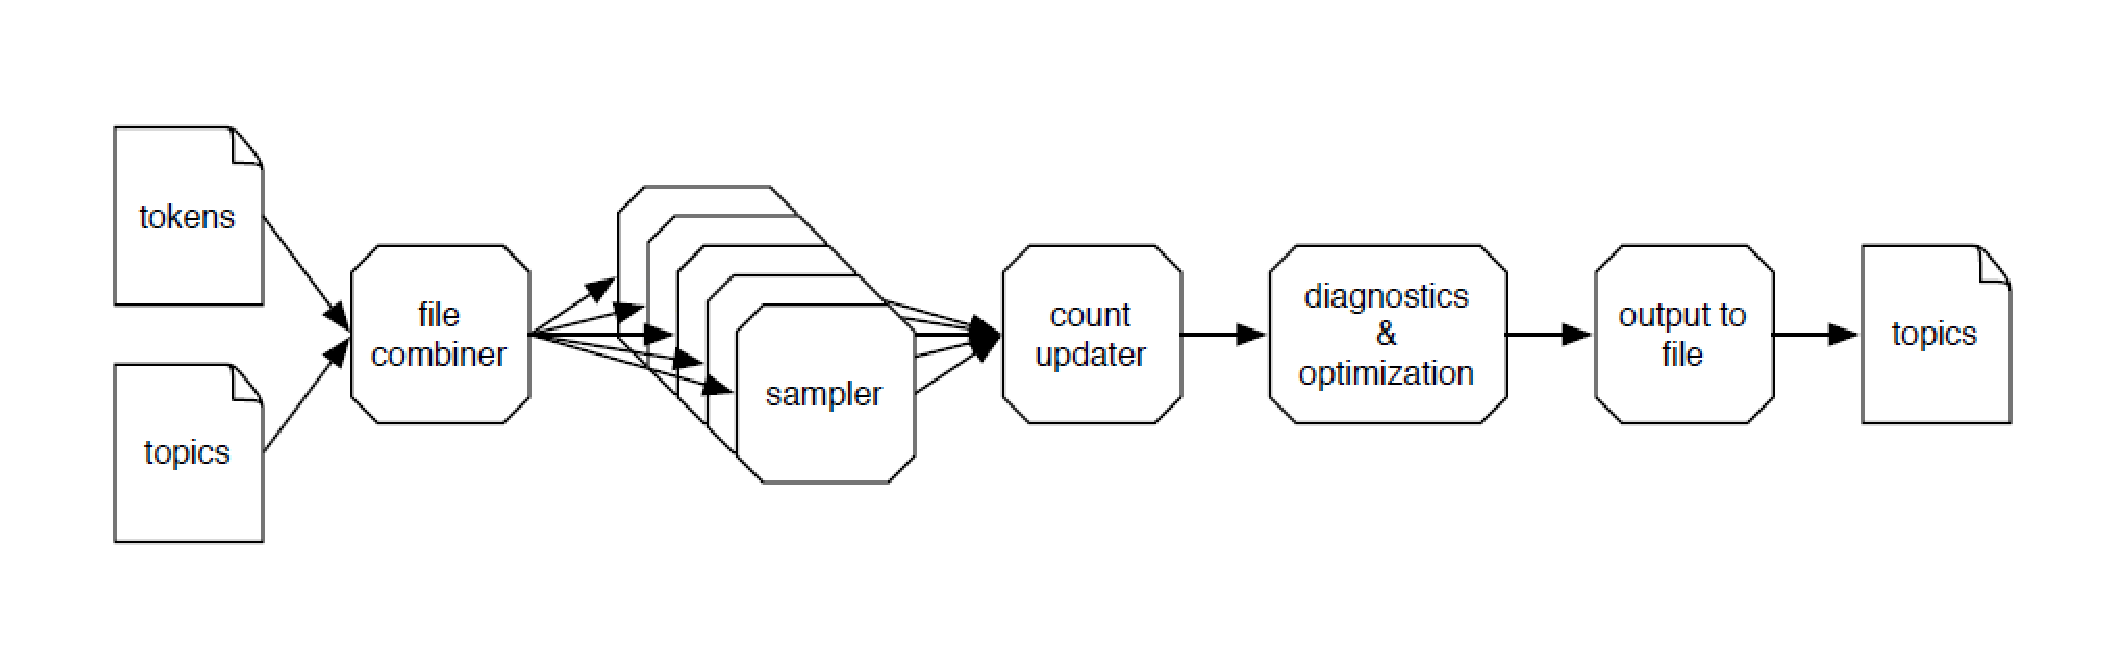
\includegraphics{data_flow}}
\end{DoxyImageNoCaption}
 
\item {\bfseries \hyperlink{class_synchronized___training___execution___strategy}{Synchronized\_\-Training\_\-Execution\_\-Strategy}:}\par
 The default implementation of \hyperlink{class_execution___strategy}{Execution\_\-Strategy} that extends \hyperlink{class_training___execution___strategy}{Training\_\-Execution\_\-Strategy} and adds Synchronization capability 
\item {\bfseries \hyperlink{class_testing___execution___strategy}{Testing\_\-Execution\_\-Strategy}:}\par
 The default implementation of \hyperlink{class_execution___strategy}{Execution\_\-Strategy} for LDA testing.


\end{DoxyEnumerate}\hypertarget{architecture_unigram}{}\section{Unigram Model}\label{architecture_unigram}
The framework also provides the \hyperlink{class_unigram___model}{Unigram\_\-Model} implementations of the various common interfaces. This is the basic LDA model with the bag of words assumption. Please take a look at how the various interfaces are implemented. The main implementation needed is for \hyperlink{class_model}{Model} \& \hyperlink{class_model___refiner}{Model\_\-Refiner}. Additionally, it implements efficient sparse data structures to store the sufficient statistics.\hypertarget{architecture_new_model}{}\section{Adding a new Model}\label{architecture_new_model}
Please use the \hyperlink{class_unigram___model}{Unigram\_\-Model} implementation as an example to implement new models\hypertarget{architecture_chkpt}{}\section{Checkpoints}\label{architecture_chkpt}
The framework also provide checkpointing functionality for the multi-\/machine setup in order to provide failure recovery. This is implemented by an external object that knows how to do three things: a. Serialize metadata to disk b. load previously serialized metadata on request c. Serialize the datastructures to disk

An appropriate checkpointer is passed as an argument while creating an \hyperlink{class_execution___strategy}{Execution\_\-Strategy} The strategy uses checkpointers to checkpoint at regular intervals. At startup, it also checks if any checkpoints are available and if so, it starts up from that checkpoint.

Different checkpointers are needed for different setups. For ex., the framework uses the Local \hyperlink{class_checkpointer}{Checkpointer} when running in single machine mode which only involves writing the iteration number as metadata. All other data needed for restart is already being serialized. However, for the multi-\/machine setup, a different mechanism is needed and a Hadoop \hyperlink{class_checkpointer}{Checkpointer} is implemented.

This is an ongoing effort and we will add more stuff both to the code and documentation. We definitely need your help \& contribution in making this better.

Here is an initial set of TODOs:

\begin{Desc}
\item[\hyperlink{todo__todo000001}{Todo}]Add unit tests to make the code more robust 

Add more code documentation for the \hyperlink{class_unigram___model}{Unigram\_\-Model} components 

Implement fancier models in later versions 

Implement extensions to the LDA model in later versions\end{Desc}
These are in no particular order and we might re-\/prioritize later. Please mail me if you are interested in contributing

We shall use the git pull request (fork + pull model) for collaborative development. 
\chapter{Multi-\/Machine Setup}
\label{multi_machine_usage}
\hypertarget{multi_machine_usage}{}
Please take a look at \hyperlink{single__machine__usage}{Single Machine Usage} for information on running individual commands. Here we give you ways to run those individual commands on multiple machines. So, we are not repeating the details on the individual commands. 
\begin{DoxyEnumerate}
\item 

{\bfseries Using Hadoop} 
\begin{DoxyEnumerate}
\item 

Organize your corpus on HDFS: 
\begin{DoxyEnumerate}
\item 

Run {\ttfamily splitter.sh "queue" "orig-\/corpus" "organized-\/corpus" "chunks"} 

The splitter program is a simple map-\/reduce streaming script that splits your original corpus into chunks gzip files. This enables Y!LDA to process one chunk on one machine. We advise you to use one full machine to run one instance of Y!LDA as the memory requirements may be large depending on your corpus size. A very large corpus of the order of 10 to 20 Million moderately sized documents can need anywhere from 5 to 6 GB of memory. You can reduce this by using more machines though. For ex., if you have a corpus of 1.5 Million documents you might want to split it across 8 machines using: 

{\ttfamily splitter.sh "queue" "orig-\/corpus" "organized-\/corpus" 8} 
\end{DoxyEnumerate}
\item 

Run Y!LDA on the organized corpus: 
\begin{DoxyEnumerate}
\item 

Assuming you have a homogenous setup, install Y!LDA on one machine. 
\item 

Run make jar to create LDALibs.jar file with all the required libraries and binaries 
\item 

Copy LDALibs.jar to HDFS 
\item 

Figure out the max memory allowed per map task for your cluster and use the same in the script via the maxmem parameter. This can be done by looking at any job conf (job.xml) and searching the value of "mapred.cluster.max.map.memory.mb" property. 
\item 

Run {\ttfamily runLDA.sh 1 "flags" \mbox{[}train$|$test\mbox{]} "queue" "organized-\/corpus" "output-\/dir" "max-\/mem" "topics" "iters" "full\_\-hdfs\_\-path\_\-of\_\-LDALibs.jar" \mbox{[}"training-\/output"\mbox{]} }  
\item 

This starts a map-\/only script on each machine. The script starts the \hyperlink{class_d_m___server}{DM\_\-Server} on all the machines. Then Y!LDA is run on each machine. The input is one chunk of the corpus. 
\item 

For testing, use the test flag and provide directory storing the training output. 
\end{DoxyEnumerate}
\item 

Output generated 
\begin{DoxyEnumerate}
\item 

Creates $<$chunks$>$ folders in $<$output-\/dir$>$ one for each client.  
\item 

Each of these directories hold the same output as the single machine case but from different clients.  
\item 

$<$output-\/dir$>$/$<$client-\/id$>$/learntopics.WARNING contains the output written to stderr by client $<$client-\/id$>$ 
\item 

$<$output-\/dir$>$/$<$client-\/id$>$/lda.docToTop.txt contains the topic proportions assigned to the documents in the portion of the corpus alloted to client $<$client-\/id$>$ 
\item 

$<$output-\/dir$>$/$<$client-\/id$>$/lda.topToWor.txt contains the salient words learned for each topic. This remains almost same across clients. So you can pick one of these as the salient words per topic for the full corpus. 
\item 

$<$output-\/dir$>$/$<$client-\/id$>$/lda.ttc.dump contains the actual model. Even this like the salient words is almost same across clients and any one can be used as the model for the full corpus. 
\item 

$<$output-\/dir$>$/global contains the dump of the global dictionary and the partitioned gobal topic counts table. These are generated in the training phase and are critical for the test option to work. 
\end{DoxyEnumerate}
\item 

Viewing progress 
\begin{DoxyEnumerate}
\item 

The stderr output of the code will be redirected into hadoop logs. So you can check the task logs from the tracking URL displayed in the output of runLDA.sh to see what is happening 
\end{DoxyEnumerate}
\item 

Failure Recovery 

We provide a check-\/pointing mechanism to handle recovery from failures. The current scheme works in local mode and for distributed mode using Hadoop. The reason for this being that the distributed check-\/pointing uses the hdfs to store the check-\/points. The following is the process:  
\begin{DoxyEnumerate}
\item The formatter task is run on the inputs and the formatted input is stored in a temporary location. 
\item The learntopics task is run using the temporary location as an input and the specified output as the output directory. Care is taken to start the same number of mappers for both the formatter and learntopics tasks. The input is a dummy directory structure with dummy directories equal to the number of mappers. 
\item Each learntopics task copies its portion of the formatted input by dfs copy\_\-to\_\-local the folder corresponding to its mapred\_\-task\_\-partition. 
\item Runs learntopics with the temporary directory containing the formatted input as a check-\/point directory. So all information needed to start learntopics from the previous check-\/pointed iteration is available locally and any progress made is written back to the temporary input directory. 
\end{DoxyEnumerate}

This mechanism is utilized by the scripts to detect failure cases and attempt to re-\/run the task again from the previous checkpoint. As learntopics is designed to check if check-\/point metadata is available in the working directory and use it to start-\/off from there a separate restart option is obviated.  

As a by product one gets the facility of doing incremental runs, that is, to run say 100 iterations, check the output and run the next 100 iterations if needed. The scripts detect this condition and ask you if you want to start-\/off from where you left or restart from the beginning. 

The scripts are designed in such a fashion that these happen transparently to the user. This is information for developers and for cases where the recovery mechanism could not handle the failure in the specified number of attempts. Check the stderr logs to see what the reason for failure is. Most times it is due to wrong usage which results in unrecoverable aborts. If you think its because of a flaky cluster, then try increasing the number of attempts. If nothing works and you think there is a bug in the code please let us know. 
\end{DoxyEnumerate}
\end{DoxyEnumerate}
\begin{DoxyEnumerate}
\item 

{\bfseries Using SSH -\/ Assume you have 'm' machines} 
\begin{DoxyEnumerate}
\item 

If you have a homogenous set up, install Y!LDA on one machine, run make jar and copy LDALibs.jar to all the other machines in the set up. Else install Y!LDA on all machines. 
\item 

Split the corpus into 'm' parts and distribute them to the 'm' machines 
\item 

Run formatter on each split of the corpus on every machine. 
\item 

Run the Distributed\_\-Map Server on each machine as a background process using nohup: 

{\ttfamily nohup ./DM\_\-Server $<$model$>$ $<$server\_\-id$>$ $<$num\_\-clients$>$ $<$host:port$>$ -\/-\/Ice.ThreadPool.Server.SizeMax=9 \&} 
\begin{DoxyEnumerate}
\item 

model: an integer that represents the model. Set it to 1 for \hyperlink{class_unigram___model}{Unigram\_\-Model} 
\item 

server\_\-id: a number that denotes the index of this server in the list of servers that is provided to 'learntopics'. If server1 has h:p, 10.1.1.1:10000 \& is assigned id 0, server2 has h:p, 10.1.1.2:10000 \& is assigned id 1, the list of servers that is provided to 'learntopics' has to be 10.1.1.1:10000, 10.1.1.2:10000 and not the other way around. 
\item 

num\_\-clients: a number that denotes the number of clients that will access the Distributed Map. This is usually equal to 'm'. This is used to provide a barrier implementation 
\item 

host:port-\/ the port and ip address on which the server must listen on 
\end{DoxyEnumerate}
\item 

Run Y!LDA on the corpus: 
\begin{DoxyEnumerate}
\item 

{\ttfamily learntopics -\/-\/topics=$<$topics$>$ -\/-\/iter=$<$iter$>$ -\/-\/servers=$<$list-\/of-\/servers$>$ -\/-\/chkptdir="/tmp" -\/-\/chkptinterval=10000} 
\begin{DoxyEnumerate}
\item 

$<$list-\/of-\/servers$>$: The comma separated list of ip:port numbers of the servers involved in the set-\/up. The index of the ip:port numbers should be as per the server\_\-id parameter used in starting the server 
\item 

chkptdir \& chkptinterval: These are currently used only with the Hadoop set-\/up. Set chkptdir to something dummy. In order that the checkpointing code does not execute, set the chkptinterval to a very large value or some number greater than the number of iterations 
\end{DoxyEnumerate}
\item 

Create Global Dictionary -\/ Run the following on server with id 0. Assuming learntopics was run in the folder /tmp/corpus 
\begin{DoxyEnumerate}
\item 

{\ttfamily mkdir -\/p /tmp/corpus/global\_\-dict; cd /tmp/corpus/global\_\-dict;} 
\item 

{\ttfamily scp server\_\-i:/tmp/corpus/lda.dict.dump lda.dict.dump.i } where the variable 'i' is the same as the server\_\-id. 
\item 

Merge Dictionaries\par
 {\ttfamily Merge\_\-Dictionaries -\/-\/dictionaries=m -\/-\/dumpprefix=lda.dict.dump} 
\item 

{\ttfamily mkdir -\/p ../global; mkdir -\/p ../global/topic\_\-counts; cp lda.dict.dump ../global/;}  
\end{DoxyEnumerate}
\item 

Create a sharded Global Word-\/Topic Counts dump -\/ Run on every machine in the set-\/up 
\begin{DoxyEnumerate}
\item 

{\ttfamily mkdir -\/p /tmp/corpus/global\_\-top\_\-cnts; cd /tmp/corpus/global\_\-top\_\-cnts;} 
\item 

{\ttfamily scp server\_\-0:/tmp/corpus/global/lda.dict.dump lda.dict.dump.global} 
\item 

{\ttfamily Merge\_\-Topic\_\-Counts -\/-\/topics=$<$topics$>$ -\/-\/clientid=$<$server-\/id$>$ -\/-\/servers=$<$list-\/of-\/servers$>$ -\/-\/globaldictionary="lda.dict.dump.global"} 
\item 

{\ttfamily scp lda.ttc.dump server\_\-0:/tmp/corpus/global/topic\_\-counts/lda.ttc.dump.\$server-\/id} 
\end{DoxyEnumerate}
\item 

Copy the parameters dump file to global dump -\/ Run on server\_\-0 
\begin{DoxyEnumerate}
\item 

{\ttfamily cd /tmp/corpus; cp lda.par.dump global/topic\_\-counts/lda.par.dump} 
\end{DoxyEnumerate}
\item 

This completes training and the model is available on server\_\-0:/tmp/corpus/global 
\end{DoxyEnumerate}
\item 

Running Y!LDA is test mode: Run on server\_\-0. Assuming test corpus is in /tmp/test\_\-corpus 
\begin{DoxyEnumerate}
\item 

{\ttfamily cd /tmp/test\_\-corpus;}  
\item 

{\ttfamily cp -\/r ../corpus/global .} 
\item 

{\ttfamily learntopics -\/teststream -\/-\/dumpprefix=global/topic\_\-counts/lda -\/-\/numdumps=m -\/-\/dictionary=global/lda.dict.dump -\/-\/maxmemory=2048 -\/-\/topics=$<$topics$>$} 
\item 

cat all your documents, in the same format that 'formatter' expects, to the above command's stdin 
\end{DoxyEnumerate}
\end{DoxyEnumerate}
\end{DoxyEnumerate}
\chapter{Single Machine Setup}
\label{single_machine_usage}
\hypertarget{single_machine_usage}{}
First step is to set LD\_\-LIBRARY\_\-PATH. This can be done by sourcing the script setLibVars.sh 

Assume Y!LDA is installed in \$LDA\_\-HOME. 

cd \$LDA\_\-HOME 

source ./setLibVars.sh \subsubsection*{Basic Usage: }


\begin{DoxyEnumerate}
\item \hyperlink{single__machine__usage_learning_model}{Learning a Model} 
\item \hyperlink{single__machine__usage_using_model}{Using the Model} 
\item \hyperlink{single__machine__usage_generated_output}{Output Generated} 
\item \hyperlink{single__machine__usage_customizations}{Customization} 
\end{DoxyEnumerate}\hypertarget{single__machine__usage_learning_model}{}\section{Learning a Model}\label{single__machine__usage_learning_model}
The process of learning a model has four steps: 
\begin{DoxyEnumerate}
\item \hyperlink{single__machine__usage_tokenize_format}{Tokenization and Formatting}  
\item \hyperlink{single__machine__usage_learntopics}{Learning the topic mixtures}  
\item \hyperlink{single__machine__usage_word_mix}{Viewing the word mixtures for each topic}  
\item \hyperlink{single__machine__usage_topic_mix}{Viewing the topic assignments}  
\end{DoxyEnumerate}\hypertarget{single__machine__usage_tokenize_format}{}\subsection{Tokenization and Formatting}\label{single__machine__usage_tokenize_format}
The tokenizer converts text into tokens that undergone some basic normalizations. Most likely you want to write your own. A Java version is provided for convenience more than anything else. This is a simple java class that tokenizes the file by splitting the stream around non-\/character\mbox{[}$^\wedge$a-\/zA-\/Z\mbox{]} boundaries into word tokens. So, it ignores numbers \& punctuation currently. The raw text corpus is assumed to have the following format. Its a single file containing documents on every line. Each document has the format: 

doc-\/id$<$space$>$aux-\/id$<$space$>$word1\mbox{[}$<$space$>$word2\mbox{]}$\ast$ 

The tokenizer just writes the tokens appended to the {\bfseries doc-\/id} \& {\bfseries aux-\/id} to stdout. 

The 'formatter' converts the text into GoogleProtocolBuffer messages. This is done to ensure that we have a very small file footprint on disk. It takes the tokenized corpus supplied as input and formats it into the internal format needed for learntopics. The primary output is the documents in the internal format. The program by default removes stop words supplied statically in the \hyperlink{constants_8h}{src/commons/constants.h} file. It then creates the dictionary from the remaining words. 

The following is an illustration of this step. It uses the taining set that is available with the package (ut\_\-out/ydir\_\-1k.txt) 

\par
  {\ttfamily  }

{\ttfamily \$ cd \$LDA\_\-HOME/ut\_\-out }

{\ttfamily \$ cp ../Tokenizer.java . }

{\ttfamily \$ javac Tokenizer.java }

{\ttfamily \$ ls -\/al ydir\_\-1k.txt }

{\ttfamily -\/rw-\/r-\/-\/r-\/-\/ 1 shravanm shravanm 1818848 2011-\/04-\/17 17:34 ydir\_\-1k.txt  }

{\ttfamily \$ cat ydir\_\-1k.txt $|$ java Tokenizer $|$ ../formatter }

{\ttfamily W0417 17:35:44.967370 19605 Controller.cpp:83\mbox{]} -\/-\/-\/-\/-\/-\/-\/-\/-\/-\/-\/-\/-\/-\/-\/-\/-\/-\/-\/-\/-\/-\/-\/-\/-\/-\/-\/-\/-\/-\/-\/-\/-\/-\/-\/-\/-\/-\/-\/-\/-\/-\/-\/-\/-\/-\/-\/-\/-\/-\/-\/-\/-\/-\/-\/-\/-\/-\/-\/-\/-\/-\/-\/-\/-\/-\/-\/-\/-\/-\/}

{\ttfamily   }

{\ttfamily W0417 17:35:44.967788 19605 Controller.cpp:84\mbox{]} Log files are being stored at /home/shravanm/workspace/LDA\_\-Refactored/ut\_\-out/unigram/formatter.$\ast$}

{\ttfamily   }

{\ttfamily W0417 17:35:44.967808 19605 Controller.cpp:85\mbox{]} -\/-\/-\/-\/-\/-\/-\/-\/-\/-\/-\/-\/-\/-\/-\/-\/-\/-\/-\/-\/-\/-\/-\/-\/-\/-\/-\/-\/-\/-\/-\/-\/-\/-\/-\/-\/-\/-\/-\/-\/-\/-\/-\/-\/-\/-\/-\/-\/-\/-\/-\/-\/-\/-\/-\/-\/-\/-\/-\/-\/-\/-\/-\/-\/-\/-\/-\/-\/-\/-\/}

{\ttfamily   }

{\ttfamily W0417 17:35:44.968111 19605 Controller.cpp:91\mbox{]} Assuming that corpus is being piped through stdin. Reading from stdin...  }

{\ttfamily W0417 17:35:45.652430 19605 Controller.cpp:107\mbox{]} Formatting Complete. Formatted document stored in lda.wor. You have used lda as the output prefix. Make sure you use the same as the input prefix for learntopics  }

{\ttfamily W0417 17:35:45.652497 19605 Controller.cpp:113\mbox{]} Dumping dictionary for later use by learntopics into lda.dict.dump  }

{\ttfamily W0417 17:35:45.674201 19605 Controller.cpp:117\mbox{]} Finished dictionary dump  }

{\ttfamily W0417 17:35:45.674236 19605 Controller.cpp:118\mbox{]} Formatting done  }

{\ttfamily W0417 17:35:45.674253 19605 Controller.cpp:122\mbox{]} Total number of unique words found: 17208  }

{\ttfamily W0417 17:35:45.674270 19605 Controller.cpp:123\mbox{]} Total num of docs found: 900  }

{\ttfamily W0417 17:35:45.674288 19605 Controller.cpp:124\mbox{]} Total num of tokens found: 182525 }

{\ttfamily \$ ls -\/1 lda$\ast$ }

{\ttfamily -\/rw-\/r-\/-\/r-\/-\/ 1 shravanm shravanm 204655 2011-\/04-\/17 17:35 lda.dict.dump  }

{\ttfamily -\/rw-\/r-\/-\/r-\/-\/ 1 shravanm shravanm 397983 2011-\/04-\/17 17:35 lda.wor  } 

\par
  \hypertarget{single__machine__usage_learntopics}{}\subsection{Learning the topic mixtures}\label{single__machine__usage_learntopics}
'learntopics' learns a topic model from a corpus which has been formatted using 'formatter'. The input to this are the files generated by 'formatter'. So you need to run this in the same directory that contains these files. The output from this step contains two types of files: binary files that are used by other modes of operation like batch and stream mode testing and text files which are human readable and give a sense of what has happened. The generated output will be explained in detail in the next sections. But the primary outputs are the topic assignments to the documents in the corpus and the word mixtures that represent each topic that has been learnt. 

Continuing with the illustration of step 1 we do the following to learn the model: Assuming that PWD=\$LDA\_\-HOME/ut\_\-out {\ttfamily  }

{\ttfamily \$ ../learntopics -\/-\/topics=100 -\/-\/iter=500 }

{\ttfamily Log file created at: 2011/04/17 17:44:04  }

{\ttfamily Running on machine: offerenjoy  }

{\ttfamily Log line format: \mbox{[}IWEF\mbox{]}mmdd hh:mm:ss.uuuuuu threadid \href{file:line] msg}{\tt file:line\mbox{]} msg}  }

{\ttfamily W0417 17:44:04.082424 19628 Controller.cpp:68\mbox{]} -\/-\/-\/-\/-\/-\/-\/-\/-\/-\/-\/-\/-\/-\/-\/-\/-\/-\/-\/-\/-\/-\/-\/-\/-\/-\/-\/-\/-\/-\/-\/-\/-\/-\/-\/-\/-\/-\/-\/-\/-\/-\/-\/-\/-\/-\/-\/-\/-\/-\/-\/-\/-\/-\/-\/-\/-\/-\/-\/-\/-\/-\/-\/-\/-\/-\/-\/-\/-\/-\/}

{\ttfamily   }

{\ttfamily W0417 17:44:04.082855 19628 Controller.cpp:69\mbox{]} Log files are being stored at /home/shravanm/workspace/LDA\_\-Refactored/ut\_\-out/unigram/learntopics  }

{\ttfamily W0417 17:44:04.082871 19628 Controller.cpp:70\mbox{]} -\/-\/-\/-\/-\/-\/-\/-\/-\/-\/-\/-\/-\/-\/-\/-\/-\/-\/-\/-\/-\/-\/-\/-\/-\/-\/-\/-\/-\/-\/-\/-\/-\/-\/-\/-\/-\/-\/-\/-\/-\/-\/-\/-\/-\/-\/-\/-\/-\/-\/-\/-\/-\/-\/-\/-\/-\/-\/-\/-\/-\/-\/-\/-\/-\/-\/-\/-\/-\/-\/}

{\ttfamily   }

{\ttfamily W0417 17:44:04.083418 19628 Controller.cpp:81\mbox{]} You have chosen single machine training mode  }

{\ttfamily W0417 17:44:04.083976 19628 \hyperlink{_unigram___model___training___builder_8cpp}{Unigram\_\-Model\_\-Training\_\-Builder.cpp}:43\mbox{]} Initializing Dictionary from lda.dict.dump  }

{\ttfamily W0417 17:44:04.137420 19628 \hyperlink{_unigram___model___training___builder_8cpp}{Unigram\_\-Model\_\-Training\_\-Builder.cpp}:45\mbox{]} Dictionary Initialized  }

{\ttfamily W0417 17:44:04.174685 19628 \hyperlink{_unigram___model___trainer_8cpp}{Unigram\_\-Model\_\-Trainer.cpp}:24\mbox{]} Initializing Word-\/Topic counts table from docs lda.wor, lda.top using 17208 words \& 100 topics.  }

{\ttfamily W0417 17:44:04.250243 19628 \hyperlink{_unigram___model___trainer_8cpp}{Unigram\_\-Model\_\-Trainer.cpp}:26\mbox{]} Initialized Word-\/Topic counts table  }

{\ttfamily W0417 17:44:04.250313 19628 \hyperlink{_unigram___model___trainer_8cpp}{Unigram\_\-Model\_\-Trainer.cpp}:29\mbox{]} Initializing Alpha vector from Alpha\_\-bar = 50  }

{\ttfamily W0417 17:44:04.250356 19628 \hyperlink{_unigram___model___trainer_8cpp}{Unigram\_\-Model\_\-Trainer.cpp}:31\mbox{]} Alpha vector initialized  }

{\ttfamily W0417 17:44:04.250375 19628 \hyperlink{_unigram___model___trainer_8cpp}{Unigram\_\-Model\_\-Trainer.cpp}:34\mbox{]} Initializing Beta \hyperlink{struct_parameter}{Parameter} from specified Beta = 0.01  }

{\ttfamily W0417 17:44:04.250395 19628 \hyperlink{_unigram___model___trainer_8cpp}{Unigram\_\-Model\_\-Trainer.cpp}:37\mbox{]} Beta param initialized  }

{\ttfamily W0417 17:44:04.251711 19628 \hyperlink{_training___execution___strategy_8cpp}{Training\_\-Execution\_\-Strategy.cpp}:35\mbox{]} Starting Parallel training \hyperlink{class_pipeline}{Pipeline}  }

{\ttfamily W0417 17:44:04.590452 19628 \hyperlink{_training___execution___strategy_8cpp}{Training\_\-Execution\_\-Strategy.cpp}:53\mbox{]} Iteration 1 done. Took 0.00564301 mins  }

{\ttfamily W0417 17:44:04.700546 19628 \hyperlink{_unigram___model_8cpp}{Unigram\_\-Model.cpp}:92\mbox{]} Average num of topics assigned per word = 4.17091  }

{\ttfamily W0417 17:44:04.700599 19628 \hyperlink{_training___execution___strategy_8cpp}{Training\_\-Execution\_\-Strategy.cpp}:58\mbox{]} $>$$>$$>$$>$$>$$>$$>$$>$$>$$>$ Log-\/Likelihood (model, doc, total): -\/1.47974e+06 , -\/815572 , -\/2.29531e+06  }

{\ttfamily W0417 17:44:04.703927 19628 \hyperlink{_unigram___model___trainer_8cpp}{Unigram\_\-Model\_\-Trainer.cpp}:478\mbox{]} Restarting IO  }

{\ttfamily W0417 17:44:04.992218 19628 \hyperlink{_training___execution___strategy_8cpp}{Training\_\-Execution\_\-Strategy.cpp}:53\mbox{]} Iteration 2 done. Took 0.00477359 mins  }

{\ttfamily W0417 17:44:04.995560 19628 \hyperlink{_unigram___model___trainer_8cpp}{Unigram\_\-Model\_\-Trainer.cpp}:478\mbox{]} Restarting IO  }

{\ttfamily W0417 17:44:05.261360 19628 \hyperlink{_training___execution___strategy_8cpp}{Training\_\-Execution\_\-Strategy.cpp}:53\mbox{]} Iteration 3 done. Took 0.00439862 mins  }

{\ttfamily W0417 17:44:05.264669 19628 \hyperlink{_unigram___model___trainer_8cpp}{Unigram\_\-Model\_\-Trainer.cpp}:478\mbox{]} Restarting IO  }

{\ttfamily W0417 17:44:05.516330 19628 \hyperlink{_training___execution___strategy_8cpp}{Training\_\-Execution\_\-Strategy.cpp}:53\mbox{]} Iteration 4 done. Took 0.00416395 mins  }

{\ttfamily ... }

{\ttfamily ... }

{\ttfamily W0417 17:45:59.021239 19628 \hyperlink{_unigram___model___trainer_8cpp}{Unigram\_\-Model\_\-Trainer.cpp}:478\mbox{]} Restarting IO  }

{\ttfamily W0417 17:45:59.242962 19628 \hyperlink{_training___execution___strategy_8cpp}{Training\_\-Execution\_\-Strategy.cpp}:53\mbox{]} Iteration 498 done. Took 0.00366346 mins  }

{\ttfamily W0417 17:45:59.246363 19628 \hyperlink{_unigram___model___trainer_8cpp}{Unigram\_\-Model\_\-Trainer.cpp}:478\mbox{]} Restarting IO  }

{\ttfamily W0417 17:45:59.469266 19628 \hyperlink{_training___execution___strategy_8cpp}{Training\_\-Execution\_\-Strategy.cpp}:53\mbox{]} Iteration 499 done. Took 0.00368553 mins  }

{\ttfamily W0417 17:45:59.472687 19628 \hyperlink{_unigram___model___trainer_8cpp}{Unigram\_\-Model\_\-Trainer.cpp}:478\mbox{]} Restarting IO  }

{\ttfamily W0417 17:45:59.513748 19628 \hyperlink{_training___execution___strategy_8cpp}{Training\_\-Execution\_\-Strategy.cpp}:53\mbox{]} Iteration 500 done. Took 0.000653982 mins  }

{\ttfamily W0417 17:45:59.616693 19628 \hyperlink{_unigram___model_8cpp}{Unigram\_\-Model.cpp}:92\mbox{]} Average num of topics assigned per word = 1.85268  }

{\ttfamily W0417 17:45:59.616768 19628 \hyperlink{_training___execution___strategy_8cpp}{Training\_\-Execution\_\-Strategy.cpp}:58\mbox{]} $>$$>$$>$$>$$>$$>$$>$$>$$>$$>$ Log-\/Likelihood (model, doc, total): -\/1.04167e+06 , -\/425400 , -\/1.46707e+06  }

{\ttfamily W0417 17:45:59.620058 19628 \hyperlink{_unigram___model___trainer_8cpp}{Unigram\_\-Model\_\-Trainer.cpp}:478\mbox{]} Restarting IO  }

{\ttfamily W0417 17:45:59.622022 19628 \hyperlink{_training___execution___strategy_8cpp}{Training\_\-Execution\_\-Strategy.cpp}:66\mbox{]} $>$$>$$>$$>$$>$$>$$>$$>$$>$$>$$>$ Check Pointing at iteration: 500  }

{\ttfamily W0417 17:45:59.625076 19628 \hyperlink{_training___execution___strategy_8cpp}{Training\_\-Execution\_\-Strategy.cpp}:72\mbox{]} Parallel training \hyperlink{class_pipeline}{Pipeline} done  }

{\ttfamily W0417 17:45:59.625128 19628 Controller.cpp:128\mbox{]} \hyperlink{class_model}{Model} has been learnt  }

{\ttfamily W0417 17:45:59.627476 19628 \hyperlink{_unigram___model_8cpp}{Unigram\_\-Model.cpp}:105\mbox{]} Saving model for test pipeline in lda.ttc.dump and lda.par.dump  }

{\ttfamily W0417 17:45:59.695773 19628 \hyperlink{_unigram___model_8cpp}{Unigram\_\-Model.cpp}:108\mbox{]} \hyperlink{class_model}{Model} saved  }

{\ttfamily W0417 17:45:59.695843 19628 \hyperlink{_unigram___model_8cpp}{Unigram\_\-Model.cpp}:117\mbox{]} Writing top words identified per topic into lda.topToWor.txt  }

{\ttfamily W0417 17:45:59.701156 19628 \hyperlink{_unigram___model_8cpp}{Unigram\_\-Model.cpp}:139\mbox{]} Word statistics per topic written  }

{\ttfamily W0417 17:45:59.701257 19628 \hyperlink{_unigram___model___training___builder_8cpp}{Unigram\_\-Model\_\-Training\_\-Builder.cpp}:126\mbox{]} Saving document to topic-\/proportions in lda.docToTop.txt  }

{\ttfamily W0417 17:45:59.701279 19628 \hyperlink{_unigram___model___training___builder_8cpp}{Unigram\_\-Model\_\-Training\_\-Builder.cpp}:127\mbox{]} Saving word to topic assignment in lda.worToTop.txt  }

{\ttfamily W0417 17:45:59.911658 19628 \hyperlink{_unigram___model___training___builder_8cpp}{Unigram\_\-Model\_\-Training\_\-Builder.cpp}:193\mbox{]} Document to topic-\/proportions saved in lda.docToTop.txt  }

{\ttfamily W0417 17:45:59.911726 19628 \hyperlink{_unigram___model___training___builder_8cpp}{Unigram\_\-Model\_\-Training\_\-Builder.cpp}:194\mbox{]} Word to topic assignment saved in lda.worToTop.txt  }

{\ttfamily \$ ls -\/al lda$\ast$ }

{\ttfamily -\/rw-\/r-\/-\/r-\/-\/ 1 shravanm shravanm 4 2011-\/04-\/17 17:45 lda.chk  }

{\ttfamily -\/rw-\/r-\/-\/r-\/-\/ 1 shravanm shravanm 204655 2011-\/04-\/17 17:35 lda.dict.dump  }

{\ttfamily -\/rw-\/r-\/-\/r-\/-\/ 1 shravanm shravanm 168223 2011-\/04-\/17 17:45 lda.docToTop.txt  }

{\ttfamily -\/rw-\/r-\/-\/r-\/-\/ 1 shravanm shravanm 816 2011-\/04-\/17 17:45 lda.par.dump  }

{\ttfamily -\/rw-\/r-\/-\/r-\/-\/ 1 shravanm shravanm 230304 2011-\/04-\/17 17:45 lda.top  }

{\ttfamily -\/rw-\/r-\/-\/r-\/-\/ 1 shravanm shravanm 38415 2011-\/04-\/17 17:45 lda.topToWor.txt  }

{\ttfamily -\/rw-\/r-\/-\/r-\/-\/ 1 shravanm shravanm 267631 2011-\/04-\/17 17:45 lda.ttc.dump  }

{\ttfamily -\/rw-\/r-\/-\/r-\/-\/ 1 shravanm shravanm 397983 2011-\/04-\/17 17:35 lda.wor  }

{\ttfamily -\/rw-\/r-\/-\/r-\/-\/ 1 shravanm shravanm 2213071 2011-\/04-\/17 17:45 lda.worToTop.txt  } \hypertarget{single__machine__usage_word_mix}{}\subsection{Viewing the word mixtures for each topic}\label{single__machine__usage_word_mix}
{\ttfamily  }

{\ttfamily \$ cat lda.topToWor.txt }

{\ttfamily Topic 0: (center,0.171509) (diving,0.110265) (scuba,0.0857668) (equipment,0.0686183) (mark,0.0637188) (olympic,0.0465703) (rescue,0.0441205) (aquatic,0.039221) (ymca,0.039221) (family,0.0367712) (ruiz,0.0343214) (dive,0.0318716) (sports,0.0294219) (divers,0.0294219) (safety,0.0294219) (minnesota,0.0294219) (orlando,0.0294219) (advanced,0.0294219) (training,0.0269721) (international,0.0245223)  }

{\ttfamily Topic 1: (beach,0.138171) (resort,0.0760789) (florida,0.0714219) (world,0.062108) (center,0.0543465) (experience,0.0527942) (vacation,0.0481372) (fl,0.0465849) (located,0.0450326) (offers,0.0450326) (holiday,0.0403757) (south,0.0403757) (rates,0.0403757) (beautiful,0.0388233) (location,0.0341664) (sea,0.0341664) (activities,0.0341664) (resorts,0.0326141) (accommodations,0.0326141) (perfect,0.0326141)  }

{\ttfamily ... }

{\ttfamily Topic 25: (surf,0.381466) (surfing,0.0727078) (surfboards,0.0573127) (surfboard,0.0547468) (board,0.0530363) (beach,0.0367858) (shop,0.0367858) (malibu,0.0350753) (longboard,0.0325094) (boards,0.0325094) (gear,0.0299435) (bags,0.022246) (travel,0.022246) (racks,0.0213907) (wetsuits,0.0205354) (clothing,0.0205354) (california,0.0196801) (lessons,0.0188248) (ocean,0.016259) (surfers,0.0154037)  }

{\ttfamily ... }

{\ttfamily Topic 35: (credit,0.101053) (card,0.0893533) (money,0.0680813) (orders,0.0670177) (make,0.060636) (mail,0.0574452) (cards,0.0563816) (valley,0.055318) (paypal,0.0521272) (accept,0.0510636) (secure,0.0468092) (purchase,0.0468092) (time,0.0372368) (apple,0.0351095) (checks,0.0351095) (email,0.0351095) (address,0.0287279) (due,0.0276643) (special,0.0255371) (people,0.0234099) }

{\ttfamily ... }

{\ttfamily Topic 43: (racquet,0.12544) (racquets,0.107418) (wilson,0.101651) (head,0.094442) (tennis,0.0908377) (prince,0.0821871) (shoes,0.0648861) (babolat,0.0367719) (pro,0.0367719) (bags,0.030284) (string,0.0266796) (men,0.0259588) (tour,0.0237961) (mp,0.0223544) (rackets,0.0223544) (ncode,0.0223544) (grips,0.0223544) (women,0.0223544) (dunlop,0.0216335) (nike,0.0194709) }

{\ttfamily ... }

{\ttfamily Topic 81: (gear,0.151097) (water,0.0828022) (swim,0.0786631) (floatation,0.0621068) (html,0.0600373) (pro,0.0579677) (exercise,0.0538286) (mask,0.0496896) (swimming,0.04762) (aqua,0.0414114) (watergearwg,0.0372724) (aquajoggeraj,0.0372724) (kids,0.0352028) (goggles,0.0331333) (zoggszoggs,0.0310637) (fins,0.0310637) (hydro,0.0289942) (snorkel,0.0269247) (snorkeling,0.0269247) (caps,0.0269247)  }

{\ttfamily ... }

{\ttfamily Topic 96: (horse,0.190855) (horses,0.126676) (riding,0.101343) (training,0.0996538) (farm,0.0785425) (equestrian,0.0667202) (dressage,0.0472978) (equine,0.0405421) (boarding,0.0380088) (show,0.0337865) (stables,0.0270309) (lessons,0.0194308) (michigan,0.0185864) (tack,0.0185864) (riders,0.0185864) (ranch,0.016053) (farms,0.0152086) (pony,0.0152086) (ponies,0.0143641) (sale,0.0135197) } \hypertarget{single__machine__usage_topic_mix}{}\subsection{Viewing the topic assignments}\label{single__machine__usage_topic_mix}
{\ttfamily  }

{\ttfamily \$ cat lda.worToTop.txt }

{\ttfamily www.teddybears.com/ recreation/toys (teddy,36) (bears,36) (enjoy,66) (teddy,36) (bears,36) (enjoy,66) (featuring,61) (teddy,36) (bears,36) (teddy,36) (bear,36) (related,77) (information,66) (everyday,38) (fun,44) (enjoy,66) (learn,2) (enter,28) (love,61) (lord,51) (god,51) (heart,48) (soul,77) (strength,80) (commandments,2) (give,13) (today,28) (hearts,61) (impress,61) (house,80) (gates,60) (deuteronomy,36) (site,66) (sponsored,77) (brown,48) (brehm,36) (bears,36) (teddy,36) (bear,36) (artists,63) (teddy,36) (bears,36) (teddy,36) (bear,36) (classifieds,61) (teddy,36) (bear,36) (clubs,77) (teddy,36) (bear,36) (events,77) (teddy,36) (bear,36) (retailers,66) (teddy,36) (bear,36) (magazines,61) (teddy,36) (bear,36) (books,66) (teddy,36) (bear,36) (history,28) (web,66) (page,66) (design,16) (graphic,61) (elements,45) (embedded,61) (html,81) (coding,48) (created,16) (copyrighted,22) (kelly,6) (brown,48) (brehm,36) (rights,16) (reserved,16)  }

{\ttfamily www.bearsbythesea.com/ recreation/toys (teddy,36) (bear,36) (store,20) (pismo,18) (beach,25) (california,25) (specialize,56) (muffy,14) (store,20) (complete,20) (collections,87) (checkout,91) (web,66) (site,66) (muffy,14) (muffy,14) (interested,66) (information,56) (price,3) (guides,77) (forums,28) (newsletters,78) (follow,56) (information,66) (link,78) (interested,66) (purchasing,4) (items,4) (follow,56) (online,20) (store,20) (link,78) (online,20) (store,20) (information,66)  }

{\ttfamily www.the-\/toybox.com recreation/toys (party,0) (supplies,38) (wiggles,56) (licensed,19) (characters,83) (jay,0) (jay,0) (jet,83) (cabbage,49) (patch,49) (play,61) (tents,59) (activity,91) (master,0) (roll,57) (building,90) (toy,83) (building,90) (racing,50) (beanie,19) (babies,13) (personalized,19) (toys,83) (requires,85) (minimum,12) (order,19) (enter,91) (coupon,90) (code,90) (good,61) (coupons,90) (mail,56) (order,19) (info,57) (order,13) (options,78) (return,4) (policy,9) (shipping,13) (rates,1) (email,56) (wiggles,0) (party,19) (supplies,38) (toys,83) (accessories,13) (jay,0) (jay,0) (jet,83) (plane,91) (party,19) (supplies,90) (toys,83) (accessories,13) (toys,83) (party,19) (supplies,90) (licensed,19) (characters,83) (toys,83) (sell,56) (free,13) (internet,85) (premier,78) (shopping,83) (network,61) (discount,13) (shopping,4) (internet,19) (click,78) (visit,66)  } \hypertarget{single__machine__usage_using_model}{}\section{Using the Model}\label{single__machine__usage_using_model}
Once the model has been trained, you can provide the binary files as a parameter to 'learntopics' to infer topic mixtures on new documents. The following illustration uses the test set that is available with the package (ut\_\-test/ydir\_\-1k.tst.txt). 

As explained in the overview, there are two modes in which the above learnt model can be used: 
\begin{DoxyEnumerate}
\item \hyperlink{single__machine__usage_batch_mode}{Batch Mode} 
\item \hyperlink{single__machine__usage_stream_mode}{Streaming Mode} 
\end{DoxyEnumerate}\hypertarget{single__machine__usage_batch_mode}{}\subsection{Batch Mode}\label{single__machine__usage_batch_mode}
Assuming that PWD=\$LDA\_\-HOME/ut\_\-test. {\ttfamily  }

{\ttfamily First Tokenize and format the test data. }

{\ttfamily \$ cp ../ut\_\-out/Tokenizer.class . }

{\ttfamily \$ cat ydir\_\-1k.tst.txt $|$ java Tokenizer $|$ ../formatter -\/-\/dumpfile=../ut\_\-out/unigram/lda.dict.dump }

{\ttfamily W0417 22:16:41.834889 20929 Controller.cpp:83\mbox{]} -\/-\/-\/-\/-\/-\/-\/-\/-\/-\/-\/-\/-\/-\/-\/-\/-\/-\/-\/-\/-\/-\/-\/-\/-\/-\/-\/-\/-\/-\/-\/-\/-\/-\/-\/-\/-\/-\/-\/-\/-\/-\/-\/-\/-\/-\/-\/-\/-\/-\/-\/-\/-\/-\/-\/-\/-\/-\/-\/-\/-\/-\/-\/-\/-\/-\/-\/-\/-\/-\/}

{\ttfamily   }

{\ttfamily W0417 22:16:41.835304 20929 Controller.cpp:84\mbox{]} Log files are being stored at /home/shravanm/workspace/LDA\_\-Refactored/ut\_\-test/formatter.$\ast$  }

{\ttfamily W0417 22:16:41.835325 20929 Controller.cpp:85\mbox{]} -\/-\/-\/-\/-\/-\/-\/-\/-\/-\/-\/-\/-\/-\/-\/-\/-\/-\/-\/-\/-\/-\/-\/-\/-\/-\/-\/-\/-\/-\/-\/-\/-\/-\/-\/-\/-\/-\/-\/-\/-\/-\/-\/-\/-\/-\/-\/-\/-\/-\/-\/-\/-\/-\/-\/-\/-\/-\/-\/-\/-\/-\/-\/-\/-\/-\/-\/-\/-\/-\/}

{\ttfamily   }

{\ttfamily W0417 22:16:41.835626 20929 Controller.cpp:91\mbox{]} Assuming that corpus is being piped through stdin. Reading from stdin...  }

{\ttfamily W0417 22:16:41.835649 20929 Controller.cpp:97\mbox{]} Will use the dictionary dump ../ut\_\-out/unigram/lda.dict.dump to load the global dictionary.  }

{\ttfamily W0417 22:16:41.836802 20929 \hyperlink{_unigram___test___data___formatter_8cpp}{Unigram\_\-Test\_\-Data\_\-Formatter.cpp}:14\mbox{]} Initializing Dictionary from ../ut\_\-out/unigram/lda.dict.dump  }

{\ttfamily W0417 22:16:41.900626 20929 \hyperlink{_unigram___test___data___formatter_8cpp}{Unigram\_\-Test\_\-Data\_\-Formatter.cpp}:16\mbox{]} Num of unique words: 17208  }

{\ttfamily W0417 22:16:42.145593 20929 Controller.cpp:107\mbox{]} Formatting Complete. Formatted document stored in lda.wor. You have used lda as the output prefix. Make sure you use the same as the input prefix for learntopics  }

{\ttfamily W0417 22:16:42.145661 20929 Controller.cpp:115\mbox{]} Induced local dictionary being dumped to lda.dict.dump  }

{\ttfamily W0417 22:16:42.150445 20929 Controller.cpp:117\mbox{]} Finished dictionary dump  }

{\ttfamily W0417 22:16:42.150481 20929 Controller.cpp:118\mbox{]} Formatting done  }

{\ttfamily W0417 22:16:42.150507 20929 Controller.cpp:122\mbox{]} Total number of unique words found: 3506  }

{\ttfamily W0417 22:16:42.150533 20929 Controller.cpp:123\mbox{]} Total num of docs found: 100  }

{\ttfamily W0417 22:16:42.150559 20929 Controller.cpp:124\mbox{]} Total num of tokens found: 16394  } 

Note the -\/-\/dumpfile flag. Here is where you provide the dictionary of words that the model knows about. Only those words in the test data set are recognized and the rest are ignored. 

\par
  {\ttfamily  }

{\ttfamily \$ ../learntopics -\/test -\/-\/dumpprefix=../ut\_\-out/unigram/lda -\/-\/topics=100 }

{\ttfamily W0417 22:22:00.932081 20947 Controller.cpp:68\mbox{]} -\/-\/-\/-\/-\/-\/-\/-\/-\/-\/-\/-\/-\/-\/-\/-\/-\/-\/-\/-\/-\/-\/-\/-\/-\/-\/-\/-\/-\/-\/-\/-\/-\/-\/-\/-\/-\/-\/-\/-\/-\/-\/-\/-\/-\/-\/-\/-\/-\/-\/-\/-\/-\/-\/-\/-\/-\/-\/-\/-\/-\/-\/-\/-\/-\/-\/-\/-\/-\/-\/}

{\ttfamily   }

{\ttfamily W0417 22:22:00.932518 20947 Controller.cpp:69\mbox{]} Log files are being stored at /home/shravanm/workspace/LDA\_\-Refactored/ut\_\-test/learntopics.$\ast$  }

{\ttfamily W0417 22:22:00.932539 20947 Controller.cpp:70\mbox{]} -\/-\/-\/-\/-\/-\/-\/-\/-\/-\/-\/-\/-\/-\/-\/-\/-\/-\/-\/-\/-\/-\/-\/-\/-\/-\/-\/-\/-\/-\/-\/-\/-\/-\/-\/-\/-\/-\/-\/-\/-\/-\/-\/-\/-\/-\/-\/-\/-\/-\/-\/-\/-\/-\/-\/-\/-\/-\/-\/-\/-\/-\/-\/-\/-\/-\/-\/-\/-\/-\/}

{\ttfamily   }

{\ttfamily W0417 22:22:00.933087 20947 Controller.cpp:92\mbox{]} You have chosen single machine testing mode  }

{\ttfamily W0417 22:22:00.933671 20947 \hyperlink{_unigram___model___training___builder_8cpp}{Unigram\_\-Model\_\-Training\_\-Builder.cpp}:43\mbox{]} Initializing Dictionary from lda.dict.dump  }

{\ttfamily W0417 22:22:00.945226 20947 \hyperlink{_unigram___model___training___builder_8cpp}{Unigram\_\-Model\_\-Training\_\-Builder.cpp}:45\mbox{]} Dictionary Initialized  }

{\ttfamily W0417 22:22:00.998955 20947 \hyperlink{_unigram___model___tester_8cpp}{Unigram\_\-Model\_\-Tester.cpp}:33\mbox{]} Initializing Word-\/Topic counts table from dump ../ut\_\-out/unigram/lda.ttc.dump using 3506 words \& 100 topics.  }

{\ttfamily W0417 22:22:01.029986 20947 \hyperlink{_unigram___model___tester_8cpp}{Unigram\_\-Model\_\-Tester.cpp}:51\mbox{]} Initialized Word-\/Topic counts table  }

{\ttfamily W0417 22:22:01.030045 20947 \hyperlink{_unigram___model___tester_8cpp}{Unigram\_\-Model\_\-Tester.cpp}:55\mbox{]} Initializing Alpha vector from dumpfile ../ut\_\-out/unigram/lda.par.dump  }

{\ttfamily W0417 22:22:01.030118 20947 \hyperlink{_unigram___model___tester_8cpp}{Unigram\_\-Model\_\-Tester.cpp}:57\mbox{]} Alpha vector initialized  }

{\ttfamily W0417 22:22:01.030144 20947 \hyperlink{_unigram___model___tester_8cpp}{Unigram\_\-Model\_\-Tester.cpp}:60\mbox{]} Initializing Beta \hyperlink{struct_parameter}{Parameter} from specified Beta = 0.01  }

{\ttfamily W0417 22:22:01.030186 20947 \hyperlink{_unigram___model___tester_8cpp}{Unigram\_\-Model\_\-Tester.cpp}:63\mbox{]} Beta param initialized  }

{\ttfamily W0417 22:22:01.036779 20947 \hyperlink{_testing___execution___strategy_8cpp}{Testing\_\-Execution\_\-Strategy.cpp}:24\mbox{]} Starting Parallel testing \hyperlink{class_pipeline}{Pipeline}  }

{\ttfamily W0417 22:22:01.329864 20947 \hyperlink{_testing___execution___strategy_8cpp}{Testing\_\-Execution\_\-Strategy.cpp}:36\mbox{]} Iteration 0 done. Took 0.00488273 mins  }

{\ttfamily W0417 22:22:01.354588 20947 \hyperlink{_unigram___model_8cpp}{Unigram\_\-Model.cpp}:92\mbox{]} Average num of topics assigned per word = 3.37222  }

{\ttfamily W0417 22:22:01.354617 20947 \hyperlink{_testing___execution___strategy_8cpp}{Testing\_\-Execution\_\-Strategy.cpp}:41\mbox{]} $>$$>$$>$$>$$>$$>$$>$$>$$>$$>$ Log-\/Likelihood (model, doc, total): -\/1.93551e+06 , -\/57496.6 , -\/1.99301e+06  }

{\ttfamily W0417 22:22:01.358059 20947 \hyperlink{_testing___execution___strategy_8cpp}{Testing\_\-Execution\_\-Strategy.cpp}:49\mbox{]} Parallel testing \hyperlink{class_pipeline}{Pipeline} done  }

{\ttfamily W0417 22:22:01.360312 20947 \hyperlink{_unigram___model_8cpp}{Unigram\_\-Model.cpp}:105\mbox{]} Saving model for test pipeline in lda.ttc.dump and lda.par.dump  }

{\ttfamily W0417 22:22:01.375068 20947 \hyperlink{_unigram___model_8cpp}{Unigram\_\-Model.cpp}:108\mbox{]} \hyperlink{class_model}{Model} saved  }

{\ttfamily W0417 22:22:01.375098 20947 \hyperlink{_unigram___model_8cpp}{Unigram\_\-Model.cpp}:117\mbox{]} Writing top words identified per topic into lda.topToWor.txt  }

{\ttfamily W0417 22:22:01.380234 20947 \hyperlink{_unigram___model_8cpp}{Unigram\_\-Model.cpp}:139\mbox{]} Word statistics per topic written  }

{\ttfamily W0417 22:22:01.380290 20947 \hyperlink{_unigram___model___training___builder_8cpp}{Unigram\_\-Model\_\-Training\_\-Builder.cpp}:126\mbox{]} Saving document to topic-\/proportions in lda.docToTop.txt  }

{\ttfamily W0417 22:22:01.380311 20947 \hyperlink{_unigram___model___training___builder_8cpp}{Unigram\_\-Model\_\-Training\_\-Builder.cpp}:127\mbox{]} Saving word to topic assignment in lda.worToTop.txt  }

{\ttfamily W0417 22:22:01.401484 20947 \hyperlink{_unigram___model___training___builder_8cpp}{Unigram\_\-Model\_\-Training\_\-Builder.cpp}:193\mbox{]} Document to topic-\/proportions saved in lda.docToTop.txt  }

{\ttfamily W0417 22:22:01.401512 20947 \hyperlink{_unigram___model___training___builder_8cpp}{Unigram\_\-Model\_\-Training\_\-Builder.cpp}:194\mbox{]} Word to topic assignment saved in lda.worToTop.txt  } 

\par
  

Note the following flags: 

1. test: This indicates the batch test mode 

2. dumpprefix: This flag gives the prefix for the binary files storing the model in our case, ../ut\_\-out/lda. 'lda' is the default prefix used by the framework when none is specified. If you have specified a different prefix here is the place to use it. This will add different suffixes to fetch the various binary files to fetch the model saved and use them to infer the topic mixture for your new documents. 

3. topics: This flag indicates the number of topics that your trained model contained. The same number should be used for your new documents. 

\par
  {\ttfamily  }

{\ttfamily \$ ls -\/al lda$\ast$ }

{\ttfamily -\/rw-\/r-\/-\/r-\/-\/ 1 shravanm shravanm 40059 2011-\/04-\/17 22:16 lda.dict.dump  }

{\ttfamily -\/rw-\/r-\/-\/r-\/-\/ 1 shravanm shravanm 204655 2011-\/04-\/17 22:16 lda.dict.dump.global  }

{\ttfamily -\/rw-\/r-\/-\/r-\/-\/ 1 shravanm shravanm 18947 2011-\/04-\/17 22:22 lda.docToTop.txt  }

{\ttfamily -\/rw-\/r-\/-\/r-\/-\/ 1 shravanm shravanm 816 2011-\/04-\/17 22:22 lda.par.dump  }

{\ttfamily -\/rw-\/r-\/-\/r-\/-\/ 1 shravanm shravanm 62380 2011-\/04-\/17 22:22 lda.top  }

{\ttfamily -\/rw-\/r-\/-\/r-\/-\/ 1 shravanm shravanm 38389 2011-\/04-\/17 22:22 lda.topToWor.txt  }

{\ttfamily -\/rw-\/r-\/-\/r-\/-\/ 1 shravanm shravanm 83799 2011-\/04-\/17 22:22 lda.ttc.dump  }

{\ttfamily -\/rw-\/r-\/-\/r-\/-\/ 1 shravanm shravanm 36374 2011-\/04-\/17 22:16 lda.wor  }

{\ttfamily -\/rw-\/r-\/-\/r-\/-\/ 1 shravanm shravanm 200546 2011-\/04-\/17 22:22 lda.worToTop.txt  }

{\ttfamily \par
  } 

This is pretty much the same output that you see when you learnt the model but for your new documents. 

\par
  \hypertarget{single__machine__usage_stream_mode}{}\subsection{Streaming Mode}\label{single__machine__usage_stream_mode}
Again assuming that PWD=\$LDA\_\-HOME/ut\_\-test 

In this there is no need for formatting the documents but you need to provide the dictionary as an additional parameter. You also need to specify the maximum memory in MBs that you can allocate to store the model. You can tokenize and directly pipe the raw text documents through 'learntopics'.  {\ttfamily  }

{\ttfamily \$ java Tokenizer $|$ ../learntopics -\/teststream -\/-\/dumpprefix=../ut\_\-out/unigram/lda -\/-\/topics=100 -\/-\/dictionary=../ut\_\-out/unigram/lda.dict.dump -\/-\/maxmem=128 }

{\ttfamily W0417 23:06:24.342099 21004 Controller.cpp:68\mbox{]} -\/-\/-\/-\/-\/-\/-\/-\/-\/-\/-\/-\/-\/-\/-\/-\/-\/-\/-\/-\/-\/-\/-\/-\/-\/-\/-\/-\/-\/-\/-\/-\/-\/-\/-\/-\/-\/-\/-\/-\/-\/-\/-\/-\/-\/-\/-\/-\/-\/-\/-\/-\/-\/-\/-\/-\/-\/-\/-\/-\/-\/-\/-\/-\/-\/-\/-\/-\/-\/-\/}

{\ttfamily   }

{\ttfamily W0417 23:06:24.342605 21004 Controller.cpp:69\mbox{]} Log files are being stored at /home/shravanm/workspace/LDA\_\-Refactored/ut\_\-test/learntopics.$\ast$  }

{\ttfamily W0417 23:06:24.342627 21004 Controller.cpp:70\mbox{]} -\/-\/-\/-\/-\/-\/-\/-\/-\/-\/-\/-\/-\/-\/-\/-\/-\/-\/-\/-\/-\/-\/-\/-\/-\/-\/-\/-\/-\/-\/-\/-\/-\/-\/-\/-\/-\/-\/-\/-\/-\/-\/-\/-\/-\/-\/-\/-\/-\/-\/-\/-\/-\/-\/-\/-\/-\/-\/-\/-\/-\/-\/-\/-\/-\/-\/-\/-\/-\/-\/}

{\ttfamily   }

{\ttfamily W0417 23:06:24.343189 21004 Controller.cpp:92\mbox{]} You have chosen single machine testing mode  }

{\ttfamily W0417 23:06:24.343723 21004 \hyperlink{_unigram___model___streaming___builder_8cpp}{Unigram\_\-Model\_\-Streaming\_\-Builder.cpp}:20\mbox{]} Initializing global dictionary from ../ut\_\-out/unigram/lda.dict.dump  }

{\ttfamily W0417 23:06:24.398543 21004 \hyperlink{_unigram___model___streaming___builder_8cpp}{Unigram\_\-Model\_\-Streaming\_\-Builder.cpp}:23\mbox{]} Dictionary initialized and has 17208  }

{\ttfamily W0417 23:06:24.398643 21004 \hyperlink{_unigram___model___streaming___builder_8cpp}{Unigram\_\-Model\_\-Streaming\_\-Builder.cpp}:49\mbox{]} Estimating the words that will fit in 128 MB  }

{\ttfamily W0417 23:06:24.486726 21004 \hyperlink{_unigram___model___streaming___builder_8cpp}{Unigram\_\-Model\_\-Streaming\_\-Builder.cpp}:52\mbox{]} 17208 will fit in 1.05881 MB of memory  }

{\ttfamily W0417 23:06:24.486809 21004 \hyperlink{_unigram___model___streaming___builder_8cpp}{Unigram\_\-Model\_\-Streaming\_\-Builder.cpp}:53\mbox{]} Initializing Local Dictionary from ../ut\_\-out/unigram/lda.dict.dump with 17208 words.  }

{\ttfamily W0417 23:06:24.562101 21004 \hyperlink{_unigram___model___streaming___builder_8cpp}{Unigram\_\-Model\_\-Streaming\_\-Builder.cpp}:82\mbox{]} Local Dictionary Initialized. Size: 34416  }

{\ttfamily W0417 23:06:24.565176 21004 \hyperlink{_unigram___model___streamer_8cpp}{Unigram\_\-Model\_\-Streamer.cpp}:27\mbox{]} Initializing Word-\/Topic counts table from dump ../ut\_\-out/unigram/lda.ttc.dump using 17208 words \& 100 topics.  }

{\ttfamily W0417 23:06:24.608408 21004 \hyperlink{_unigram___model___streamer_8cpp}{Unigram\_\-Model\_\-Streamer.cpp}:45\mbox{]} Initialized Word-\/Topic counts table  }

{\ttfamily W0417 23:06:24.608469 21004 \hyperlink{_unigram___model___streamer_8cpp}{Unigram\_\-Model\_\-Streamer.cpp}:49\mbox{]} Initializing Alpha vector from dumpfile ../ut\_\-out/unigram/lda.par.dump  }

{\ttfamily W0417 23:06:24.608543 21004 \hyperlink{_unigram___model___streamer_8cpp}{Unigram\_\-Model\_\-Streamer.cpp}:51\mbox{]} Alpha vector initialized  }

{\ttfamily W0417 23:06:24.608571 21004 \hyperlink{_unigram___model___streamer_8cpp}{Unigram\_\-Model\_\-Streamer.cpp}:54\mbox{]} Initializing Beta \hyperlink{struct_parameter}{Parameter} from specified Beta = 0.01  }

{\ttfamily W0417 23:06:24.608608 21004 \hyperlink{_unigram___model___streamer_8cpp}{Unigram\_\-Model\_\-Streamer.cpp}:57\mbox{]} Beta param initialized  }

{\ttfamily W0417 23:06:24.615538 21004 \hyperlink{_testing___execution___strategy_8cpp}{Testing\_\-Execution\_\-Strategy.cpp}:24\mbox{]} Starting Parallel testing \hyperlink{class_pipeline}{Pipeline}  }

{\ttfamily www.sauritchsurfboards.com/ recreation/sports/aquatic\_\-sports watch out jeremy sherwin is here over the past six months you may have noticed this guy in every surf magazine published jeremy is finally getting his run more.. copyright surfboards 2004 all rights reserved june 6 2004 new launches it s new and improved site you can now order custom surfboards online more improvements to come.. top selling models middot rocket fish middot speed egg middot classic middot squash  }

{\ttfamily www.sauritchsurfboards.com/ recreation/sports/aquatic\_\-sports (watch,83) (past,86) (months,77) (noticed,15) (guy,93) (surf,35) (magazine,86) (published,92) (finally,49) (run,21) (copyright,62) (surfboards,27) (rights,90) (reserved,59) (june,63) (launches,26) (improved,40) (site,26) (order,72) (custom,36) (surfboards,11) (online,68) (improvements,67) (top,29) (selling,82) (models,30) (middot,62) (rocket,23) (fish,67) (middot,35) (speed,29) (egg,2) (middot,22) (classic,58) (middot,69) (squash,67)  }

{\ttfamily www.semente.pt recreation/sports/aquatic\_\-sports por desde de 1999 para este site com o para browsers 4 ou superior de prefer ecirc ncia o internet explorer aqui gr aacute tis este site foi e pela think pink multimedia 2000 surfboards all rights reserved  }

{\ttfamily www.semente.pt recreation/sports/aquatic\_\-sports (por,83) (de,86) (para,77) (site,15) (para,93) (browsers,35) (superior,86) (de,92) (prefer,49) (internet,21) (explorer,62) (aqui,27) (gr,90) (aacute,59) (site,63) (pink,26) (multimedia,40) (surfboards,26) (rights,72) (reserved,36) }

{\ttfamily W0417 23:06:38.769309 21004 \hyperlink{_testing___execution___strategy_8cpp}{Testing\_\-Execution\_\-Strategy.cpp}:36\mbox{]} Iteration 0 done. Took 0.235894 mins  }

{\ttfamily W0417 23:06:38.875191 21004 \hyperlink{_unigram___model_8cpp}{Unigram\_\-Model.cpp}:92\mbox{]} Average num of topics assigned per word = 1.85268  }

{\ttfamily W0417 23:06:38.875252 21004 \hyperlink{_testing___execution___strategy_8cpp}{Testing\_\-Execution\_\-Strategy.cpp}:41\mbox{]} $>$$>$$>$$>$$>$$>$$>$$>$$>$$>$ Log-\/Likelihood (model, doc, total): -\/2.52084e+06 , -\/194.288 , -\/2.52103e+06  }

{\ttfamily W0417 23:06:38.875350 21004 \hyperlink{_testing___execution___strategy_8cpp}{Testing\_\-Execution\_\-Strategy.cpp}:49\mbox{]} Parallel testing \hyperlink{class_pipeline}{Pipeline} done  }

{\ttfamily \par
  } 

Note the flags used: 

1. teststream: Indicates the streaming test mode 

2. dictionary: The dictionary of words that the model knows about. Only those words in the test data set are recognized and the rest are ignored. 

3. maxmemory: In MB. Denotes the amount of memory you allocate to store the model. 

The rest are same as batch mode. 

\par
  

Here there is no other output that you need to look for. The topic assignments are dumped back to stdout. The word mixtures for the topics are the same as that in the model. \hypertarget{single__machine__usage_generated_output}{}\section{Output Generated}\label{single__machine__usage_generated_output}

\begin{DoxyEnumerate}
\item 

lda.wor: This file generated by 'formatter' is the document in the protobuffer format with words replaced by their indices 
\item 

lda.top: This file generated by 'learntopics' contains the current topic assignments for all the documents in the protobuffer format 
\item 

lda.dict.dump: This file is a binary dump of the dictionary generated by the 'formatter' program. This will be implicitly used by the 'learntopics' program 
\item 

lda.ttc.dump: This file generated by 'learntopics' is the binary dump of the word-\/topic counts table. This is the state at the end of all the iterations and essentially represents all the training that has happened through all the iterations. It is very important as this is a necessary input to the test pipeline. 
\item 

lda.par.dump: This file generated by 'learntopics' is the binary dump of the parameters specified by the user which might be modified by an optimization step 
\item 

lda.chk: This file generated by 'learntopics' is a checkpoint keeping the current iteration and some metadata 
\item 

lda.$\ast$.txt: These are for human consumption and there are three of these generated by 'learntopics': 
\begin{DoxyEnumerate}
\item 

lda.topToWor.txt – The word mixtures for each topics 
\item 

lda.worToTop.txt – The topic assignments for every document on a per word basis 
\item 

lda.docToTop.txt – The topic proportions for every document 
\end{DoxyEnumerate}
\end{DoxyEnumerate}\hypertarget{single__machine__usage_customizations}{}\section{Customization}\label{single__machine__usage_customizations}
In its simplest form, all the parameters to 'formatter' and 'learntopics' have sensible default values which practically allows them to be used without any arguments. However, if you need to customize your setup then the following options are available: 
\begin{DoxyItemize}
\item 

I/O Customization: By default all files output by the formatter, which are also the input to the learnTopcis program and all files output by the learntopics program use the prefix {\bfseries lda}. This can be easily customized using the {\bfseries outputprefix} \& {\bfseries inputprefix} flags respectively. But while this customization is used, one needs to be careful about keeping the {\bfseries outputprefix} \& {\bfseries inputprefix} same.  
\item 

\hyperlink{struct_parameter}{Parameter} Customization: The weights of the Dirichlet Conjugates for both topics(alpha) \& words(beta) can be changed by the {\bfseries alpha} \& {\bfseries beta} flags.  
\item 

Diagnostics \& Optimization: By default, the code performs alpha optimization every 25 iterations after burn in and also prints the log likelihood every 25 iterations. These are customizable using {\bfseries optimizestats}, {\bfseries printloglikelihood} \& {\bfseries burnin} flags.  
\item 

Initialization Options: By default, we do random initialization for the topic assignments in the first iteration. However, we can be a bit smarter about this. Instead of random assignments, we start out with no topic assignments and an empty word-\/topic counts tables. The sampling depends entirely on the smoothing mass for the first few documents and subsequent documents use the counts table built so far. This is similar in style to sequential monte carlo. You can use the $\backslash$'online$\backslash$' flag to signal this. We have seen that this leads to faster convergence. 
\end{DoxyItemize}
\chapter{Using Y!LDA}
\label{usage}
\hypertarget{usage}{}
\include{usage}
\chapter{Todo List}
\label{todo}
\hypertarget{todo}{}
\label{todo__todo000001}
\hypertarget{todo__todo000001}{}
 
\begin{DoxyDescription}
\item[Page \hyperlink{architecture}{Y!LDA Architecture} ]Add unit tests to make the code more robust 

Add more code documentation for the \hyperlink{class_unigram___model}{Unigram\_\-Model} components 

Implement fancier models in later versions 

Implement extensions to the LDA model in later versions


\end{DoxyDescription}
\chapter{Namespace Index}
\section{Namespace List}
Here is a list of all namespaces with brief descriptions:\begin{DoxyCompactList}
\item\contentsline{section}{\hyperlink{namespace_l_d_a_util}{LDAUtil} }{\pageref{namespace_l_d_a_util}}{}
\item\contentsline{section}{\hyperlink{namespacesampler}{sampler} }{\pageref{namespacesampler}}{}
\end{DoxyCompactList}

\chapter{Class Index}
\section{Class Hierarchy}
This inheritance list is sorted roughly, but not completely, alphabetically:\begin{DoxyCompactList}
\item \contentsline{section}{Checkpointer}{\pageref{class_checkpointer}}{}
\begin{DoxyCompactList}
\item \contentsline{section}{Local\_\-Checkpointer}{\pageref{class_local___checkpointer}}{}
\begin{DoxyCompactList}
\item \contentsline{section}{Hadoop\_\-Checkpointer}{\pageref{class_hadoop___checkpointer}}{}
\end{DoxyCompactList}
\end{DoxyCompactList}
\item \contentsline{section}{Client}{\pageref{class_client}}{}
\begin{DoxyCompactList}
\item \contentsline{section}{DM\_\-Client}{\pageref{class_d_m___client}}{}
\end{DoxyCompactList}
\item \contentsline{section}{Context}{\pageref{class_context}}{}
\item \contentsline{section}{Cookie}{\pageref{struct_cookie}}{}
\item \contentsline{section}{Data\_\-Formatter}{\pageref{class_data___formatter}}{}
\begin{DoxyCompactList}
\item \contentsline{section}{Unigram\_\-Train\_\-Data\_\-Formatter}{\pageref{class_unigram___train___data___formatter}}{}
\begin{DoxyCompactList}
\item \contentsline{section}{Unigram\_\-Model\_\-Streamer}{\pageref{class_unigram___model___streamer}}{}
\item \contentsline{section}{Unigram\_\-Test\_\-Data\_\-Formatter}{\pageref{class_unigram___test___data___formatter}}{}
\end{DoxyCompactList}
\end{DoxyCompactList}
\item GlobalTable::DistributedMap\begin{DoxyCompactList}
\item \contentsline{section}{DM\_\-Server}{\pageref{class_d_m___server}}{}
\end{DoxyCompactList}
\item \contentsline{section}{LDAUtil::DM\_\-Server\_\-Names}{\pageref{class_l_d_a_util_1_1_d_m___server___names}}{}
\item \contentsline{section}{DocumentReader}{\pageref{class_document_reader}}{}
\item \contentsline{section}{DocumentWriter}{\pageref{class_document_writer}}{}
\item \contentsline{section}{Execution\_\-Strategy}{\pageref{class_execution___strategy}}{}
\begin{DoxyCompactList}
\item \contentsline{section}{Testing\_\-Execution\_\-Strategy}{\pageref{class_testing___execution___strategy}}{}
\item \contentsline{section}{Training\_\-Execution\_\-Strategy}{\pageref{class_training___execution___strategy}}{}
\begin{DoxyCompactList}
\item \contentsline{section}{Synchronized\_\-Training\_\-Execution\_\-Strategy}{\pageref{class_synchronized___training___execution___strategy}}{}
\end{DoxyCompactList}
\end{DoxyCompactList}
\item \contentsline{section}{Filter\_\-Eval}{\pageref{class_filter___eval}}{}
\item \contentsline{section}{Filter\_\-Optimizer}{\pageref{class_filter___optimizer}}{}
\item \contentsline{section}{Filter\_\-Reader}{\pageref{class_filter___reader}}{}
\item \contentsline{section}{Filter\_\-Sampler}{\pageref{class_filter___sampler}}{}
\item \contentsline{section}{Filter\_\-Tester}{\pageref{class_filter___tester}}{}
\item \contentsline{section}{Filter\_\-Updater}{\pageref{class_filter___updater}}{}
\item \contentsline{section}{Filter\_\-Writer}{\pageref{class_filter___writer}}{}
\item \contentsline{section}{GenericTopKList$<$ T, GreaterThan $>$}{\pageref{class_generic_top_k_list}}{}
\item \contentsline{section}{Hashmap\_\-Array$<$ Key, Value $>$}{\pageref{class_hashmap___array}}{}
\item \contentsline{section}{InvalidOldTopicExc}{\pageref{class_invalid_old_topic_exc}}{}
\item \contentsline{section}{Hashmap\_\-Array$<$ Key, Value $>$::iterator}{\pageref{class_hashmap___array_1_1iterator}}{}
\item \contentsline{section}{LDAUtil::Itoa}{\pageref{class_l_d_a_util_1_1_itoa}}{}
\item \contentsline{section}{Model}{\pageref{class_model}}{}
\begin{DoxyCompactList}
\item \contentsline{section}{Unigram\_\-Model}{\pageref{class_unigram___model}}{}
\end{DoxyCompactList}
\item \contentsline{section}{Model\_\-Builder}{\pageref{class_model___builder}}{}
\begin{DoxyCompactList}
\item \contentsline{section}{Unigram\_\-Model\_\-Streaming\_\-Builder}{\pageref{class_unigram___model___streaming___builder}}{}
\item \contentsline{section}{Unigram\_\-Model\_\-Training\_\-Builder}{\pageref{class_unigram___model___training___builder}}{}
\begin{DoxyCompactList}
\item \contentsline{section}{Unigram\_\-Model\_\-Synchronized\_\-Training\_\-Builder}{\pageref{class_unigram___model___synchronized___training___builder}}{}
\item \contentsline{section}{Unigram\_\-Model\_\-Testing\_\-Builder}{\pageref{class_unigram___model___testing___builder}}{}
\end{DoxyCompactList}
\end{DoxyCompactList}
\item \contentsline{section}{Model\_\-Director}{\pageref{class_model___director}}{}
\item \contentsline{section}{Model\_\-Refiner}{\pageref{class_model___refiner}}{}
\begin{DoxyCompactList}
\item \contentsline{section}{Unigram\_\-Model\_\-Tester}{\pageref{class_unigram___model___tester}}{}
\begin{DoxyCompactList}
\item \contentsline{section}{Unigram\_\-Model\_\-Streamer}{\pageref{class_unigram___model___streamer}}{}
\end{DoxyCompactList}
\item \contentsline{section}{Unigram\_\-Model\_\-Trainer}{\pageref{class_unigram___model___trainer}}{}
\end{DoxyCompactList}
\item \contentsline{section}{Parameter}{\pageref{struct_parameter}}{}
\item \contentsline{section}{Pipeline}{\pageref{class_pipeline}}{}
\begin{DoxyCompactList}
\item \contentsline{section}{TBB\_\-Pipeline}{\pageref{class_t_b_b___pipeline}}{}
\end{DoxyCompactList}
\item \contentsline{section}{PNGCallback}{\pageref{class_p_n_g_callback}}{}
\item \contentsline{section}{PNGJob}{\pageref{class_p_n_g_job}}{}
\item \contentsline{section}{Server\_\-Helper}{\pageref{class_server___helper}}{}
\begin{DoxyCompactList}
\item \contentsline{section}{Unigram\_\-Model\_\-Server\_\-Helper}{\pageref{class_unigram___model___server___helper}}{}
\end{DoxyCompactList}
\item \contentsline{section}{simple\_\-map}{\pageref{classsimple__map}}{}
\item \contentsline{section}{LDAUtil::StringTokenizer}{\pageref{class_l_d_a_util_1_1_string_tokenizer}}{}
\item \contentsline{section}{LDAUtil::StringTrimmer}{\pageref{class_l_d_a_util_1_1_string_trimmer}}{}
\item \contentsline{section}{Synchronizer}{\pageref{class_synchronizer}}{}
\item \contentsline{section}{Synchronizer\_\-Helper}{\pageref{class_synchronizer___helper}}{}
\begin{DoxyCompactList}
\item \contentsline{section}{Unigram\_\-Model\_\-Synchronizer\_\-Helper}{\pageref{class_unigram___model___synchronizer___helper}}{}
\end{DoxyCompactList}
\item \contentsline{section}{TopicCounts}{\pageref{struct_topic_counts}}{}
\item \contentsline{section}{TopKList}{\pageref{class_top_k_list}}{}
\item \contentsline{section}{TypeTopicCounts}{\pageref{class_type_topic_counts}}{}
\item \contentsline{section}{WordIndexDictionary}{\pageref{class_word_index_dictionary}}{}
\end{DoxyCompactList}

\chapter{Class Index}
\section{Class List}
Here are the classes, structs, unions and interfaces with brief descriptions:\begin{DoxyCompactList}
\item\contentsline{section}{\hyperlink{class_checkpointer}{Checkpointer} (Used to implement failure recovery )}{\pageref{class_checkpointer}}{}
\item\contentsline{section}{\hyperlink{class_client}{Client} }{\pageref{class_client}}{}
\item\contentsline{section}{\hyperlink{class_context}{Context} (An object that maintains the context for the executing code )}{\pageref{class_context}}{}
\item\contentsline{section}{\hyperlink{struct_cookie}{Cookie} }{\pageref{struct_cookie}}{}
\item\contentsline{section}{\hyperlink{class_data___formatter}{Data\_\-Formatter} (An interface for formatter objects )}{\pageref{class_data___formatter}}{}
\item\contentsline{section}{\hyperlink{class_d_m___client}{DM\_\-Client} (The client used to access the Distributed Map )}{\pageref{class_d_m___client}}{}
\item\contentsline{section}{\hyperlink{class_d_m___server}{DM\_\-Server} (The Server class that implements the DistributedMap Ice interface )}{\pageref{class_d_m___server}}{}
\item\contentsline{section}{\hyperlink{class_l_d_a_util_1_1_d_m___server___names}{LDAUtil::DM\_\-Server\_\-Names} }{\pageref{class_l_d_a_util_1_1_d_m___server___names}}{}
\item\contentsline{section}{\hyperlink{class_document_reader}{DocumentReader} }{\pageref{class_document_reader}}{}
\item\contentsline{section}{\hyperlink{class_document_writer}{DocumentWriter} }{\pageref{class_document_writer}}{}
\item\contentsline{section}{\hyperlink{class_execution___strategy}{Execution\_\-Strategy} (Interface for strategy objects )}{\pageref{class_execution___strategy}}{}
\item\contentsline{section}{\hyperlink{class_filter___eval}{Filter\_\-Eval} (A filter in the TBB pipeline )}{\pageref{class_filter___eval}}{}
\item\contentsline{section}{\hyperlink{class_filter___optimizer}{Filter\_\-Optimizer} (A filter in the TBB pipeline )}{\pageref{class_filter___optimizer}}{}
\item\contentsline{section}{\hyperlink{class_filter___reader}{Filter\_\-Reader} (A filter in the TBB pipeline )}{\pageref{class_filter___reader}}{}
\item\contentsline{section}{\hyperlink{class_filter___sampler}{Filter\_\-Sampler} (A filter in the TBB pipeline )}{\pageref{class_filter___sampler}}{}
\item\contentsline{section}{\hyperlink{class_filter___tester}{Filter\_\-Tester} (A filter in the TBB pipeline )}{\pageref{class_filter___tester}}{}
\item\contentsline{section}{\hyperlink{class_filter___updater}{Filter\_\-Updater} }{\pageref{class_filter___updater}}{}
\item\contentsline{section}{\hyperlink{class_filter___writer}{Filter\_\-Writer} (A filter in the TBB pipeline )}{\pageref{class_filter___writer}}{}
\item\contentsline{section}{\hyperlink{class_generic_top_k_list}{GenericTopKList$<$ T, GreaterThan $>$} (A list that maintains top K elements )}{\pageref{class_generic_top_k_list}}{}
\item\contentsline{section}{\hyperlink{class_hadoop___checkpointer}{Hadoop\_\-Checkpointer} }{\pageref{class_hadoop___checkpointer}}{}
\item\contentsline{section}{\hyperlink{class_hashmap___array}{Hashmap\_\-Array$<$ Key, Value $>$} }{\pageref{class_hashmap___array}}{}
\item\contentsline{section}{\hyperlink{class_invalid_old_topic_exc}{InvalidOldTopicExc} }{\pageref{class_invalid_old_topic_exc}}{}
\item\contentsline{section}{\hyperlink{class_hashmap___array_1_1iterator}{Hashmap\_\-Array$<$ Key, Value $>$::iterator} }{\pageref{class_hashmap___array_1_1iterator}}{}
\item\contentsline{section}{\hyperlink{class_l_d_a_util_1_1_itoa}{LDAUtil::Itoa} }{\pageref{class_l_d_a_util_1_1_itoa}}{}
\item\contentsline{section}{\hyperlink{class_local___checkpointer}{Local\_\-Checkpointer} }{\pageref{class_local___checkpointer}}{}
\item\contentsline{section}{\hyperlink{class_model}{Model} }{\pageref{class_model}}{}
\item\contentsline{section}{\hyperlink{class_model___builder}{Model\_\-Builder} }{\pageref{class_model___builder}}{}
\item\contentsline{section}{\hyperlink{class_model___director}{Model\_\-Director} (The Director class of the Builder pattern )}{\pageref{class_model___director}}{}
\item\contentsline{section}{\hyperlink{class_model___refiner}{Model\_\-Refiner} }{\pageref{class_model___refiner}}{}
\item\contentsline{section}{\hyperlink{struct_parameter}{Parameter} }{\pageref{struct_parameter}}{}
\item\contentsline{section}{\hyperlink{class_pipeline}{Pipeline} (An interface that all pipeline objects must implement )}{\pageref{class_pipeline}}{}
\item\contentsline{section}{\hyperlink{class_p_n_g_callback}{PNGCallback} (The call back object for the Put and Get AMI )}{\pageref{class_p_n_g_callback}}{}
\item\contentsline{section}{\hyperlink{class_p_n_g_job}{PNGJob} }{\pageref{class_p_n_g_job}}{}
\item\contentsline{section}{\hyperlink{class_server___helper}{Server\_\-Helper} (Server Helper interface )}{\pageref{class_server___helper}}{}
\item\contentsline{section}{\hyperlink{classsimple__map}{simple\_\-map} }{\pageref{classsimple__map}}{}
\item\contentsline{section}{\hyperlink{class_l_d_a_util_1_1_string_tokenizer}{LDAUtil::StringTokenizer} }{\pageref{class_l_d_a_util_1_1_string_tokenizer}}{}
\item\contentsline{section}{\hyperlink{class_l_d_a_util_1_1_string_trimmer}{LDAUtil::StringTrimmer} }{\pageref{class_l_d_a_util_1_1_string_trimmer}}{}
\item\contentsline{section}{\hyperlink{class_synchronized___training___execution___strategy}{Synchronized\_\-Training\_\-Execution\_\-Strategy} (Default implementation of the \hyperlink{class_execution___strategy}{Execution\_\-Strategy} interface )}{\pageref{class_synchronized___training___execution___strategy}}{}
\item\contentsline{section}{\hyperlink{class_synchronizer}{Synchronizer} }{\pageref{class_synchronizer}}{}
\item\contentsline{section}{\hyperlink{class_synchronizer___helper}{Synchronizer\_\-Helper} (A helper class for the synchronizer )}{\pageref{class_synchronizer___helper}}{}
\item\contentsline{section}{\hyperlink{class_t_b_b___pipeline}{TBB\_\-Pipeline} }{\pageref{class_t_b_b___pipeline}}{}
\item\contentsline{section}{\hyperlink{class_testing___execution___strategy}{Testing\_\-Execution\_\-Strategy} }{\pageref{class_testing___execution___strategy}}{}
\item\contentsline{section}{\hyperlink{struct_topic_counts}{TopicCounts} }{\pageref{struct_topic_counts}}{}
\item\contentsline{section}{\hyperlink{class_top_k_list}{TopKList} }{\pageref{class_top_k_list}}{}
\item\contentsline{section}{\hyperlink{class_training___execution___strategy}{Training\_\-Execution\_\-Strategy} }{\pageref{class_training___execution___strategy}}{}
\item\contentsline{section}{\hyperlink{class_type_topic_counts}{TypeTopicCounts} }{\pageref{class_type_topic_counts}}{}
\item\contentsline{section}{\hyperlink{class_unigram___model}{Unigram\_\-Model} }{\pageref{class_unigram___model}}{}
\item\contentsline{section}{\hyperlink{class_unigram___model___server___helper}{Unigram\_\-Model\_\-Server\_\-Helper} }{\pageref{class_unigram___model___server___helper}}{}
\item\contentsline{section}{\hyperlink{class_unigram___model___streamer}{Unigram\_\-Model\_\-Streamer} }{\pageref{class_unigram___model___streamer}}{}
\item\contentsline{section}{\hyperlink{class_unigram___model___streaming___builder}{Unigram\_\-Model\_\-Streaming\_\-Builder} }{\pageref{class_unigram___model___streaming___builder}}{}
\item\contentsline{section}{\hyperlink{class_unigram___model___synchronized___training___builder}{Unigram\_\-Model\_\-Synchronized\_\-Training\_\-Builder} }{\pageref{class_unigram___model___synchronized___training___builder}}{}
\item\contentsline{section}{\hyperlink{class_unigram___model___synchronizer___helper}{Unigram\_\-Model\_\-Synchronizer\_\-Helper} }{\pageref{class_unigram___model___synchronizer___helper}}{}
\item\contentsline{section}{\hyperlink{class_unigram___model___tester}{Unigram\_\-Model\_\-Tester} }{\pageref{class_unigram___model___tester}}{}
\item\contentsline{section}{\hyperlink{class_unigram___model___testing___builder}{Unigram\_\-Model\_\-Testing\_\-Builder} }{\pageref{class_unigram___model___testing___builder}}{}
\item\contentsline{section}{\hyperlink{class_unigram___model___trainer}{Unigram\_\-Model\_\-Trainer} }{\pageref{class_unigram___model___trainer}}{}
\item\contentsline{section}{\hyperlink{class_unigram___model___training___builder}{Unigram\_\-Model\_\-Training\_\-Builder} }{\pageref{class_unigram___model___training___builder}}{}
\item\contentsline{section}{\hyperlink{class_unigram___test___data___formatter}{Unigram\_\-Test\_\-Data\_\-Formatter} }{\pageref{class_unigram___test___data___formatter}}{}
\item\contentsline{section}{\hyperlink{class_unigram___train___data___formatter}{Unigram\_\-Train\_\-Data\_\-Formatter} }{\pageref{class_unigram___train___data___formatter}}{}
\item\contentsline{section}{\hyperlink{class_word_index_dictionary}{WordIndexDictionary} (A two way dictionary of words to indices )}{\pageref{class_word_index_dictionary}}{}
\end{DoxyCompactList}

\chapter{File Index}
\section{File List}
Here is a list of all files with brief descriptions:\begin{DoxyCompactList}
\item\contentsline{section}{src/\hyperlink{architecture_8h}{architecture.h} }{\pageref{architecture_8h}}{}
\item\contentsline{section}{src/\hyperlink{mainpage_8h}{mainpage.h} }{\pageref{mainpage_8h}}{}
\item\contentsline{section}{src/\hyperlink{multi__mcahine__usage_8h}{multi\_\-mcahine\_\-usage.h} }{\pageref{multi__mcahine__usage_8h}}{}
\item\contentsline{section}{src/\hyperlink{single__machine__usage_8h}{single\_\-machine\_\-usage.h} }{\pageref{single__machine__usage_8h}}{}
\item\contentsline{section}{src/\hyperlink{usage_8h}{usage.h} }{\pageref{usage_8h}}{}
\item\contentsline{section}{src/commons/\hyperlink{_client_8h}{Client.h} }{\pageref{_client_8h}}{}
\item\contentsline{section}{src/commons/\hyperlink{comparator_8cpp}{comparator.cpp} }{\pageref{comparator_8cpp}}{}
\item\contentsline{section}{src/commons/\hyperlink{comparator_8h}{comparator.h} }{\pageref{comparator_8h}}{}
\item\contentsline{section}{src/commons/\hyperlink{constants_8h}{constants.h} }{\pageref{constants_8h}}{}
\item\contentsline{section}{src/commons/\hyperlink{_context_8cpp}{Context.cpp} }{\pageref{_context_8cpp}}{}
\item\contentsline{section}{src/commons/\hyperlink{_context_8h}{Context.h} }{\pageref{_context_8h}}{}
\item\contentsline{section}{src/commons/\hyperlink{document_8pb_8cc}{document.pb.cc} }{\pageref{document_8pb_8cc}}{}
\item\contentsline{section}{src/commons/\hyperlink{document_8pb_8h}{document.pb.h} }{\pageref{document_8pb_8h}}{}
\item\contentsline{section}{src/commons/\hyperlink{_document_reader_8cpp}{DocumentReader.cpp} }{\pageref{_document_reader_8cpp}}{}
\item\contentsline{section}{src/commons/\hyperlink{_document_reader_8h}{DocumentReader.h} }{\pageref{_document_reader_8h}}{}
\item\contentsline{section}{src/commons/\hyperlink{_document_writer_8cpp}{DocumentWriter.cpp} }{\pageref{_document_writer_8cpp}}{}
\item\contentsline{section}{src/commons/\hyperlink{_document_writer_8h}{DocumentWriter.h} }{\pageref{_document_writer_8h}}{}
\item\contentsline{section}{src/commons/\hyperlink{_l_d_a_util_8cpp}{LDAUtil.cpp} }{\pageref{_l_d_a_util_8cpp}}{}
\item\contentsline{section}{src/commons/\hyperlink{_l_d_a_util_8h}{LDAUtil.h} }{\pageref{_l_d_a_util_8h}}{}
\item\contentsline{section}{src/commons/\hyperlink{types_8h}{types.h} }{\pageref{types_8h}}{}
\item\contentsline{section}{src/commons/\hyperlink{_word_index_dictionary_8cpp}{WordIndexDictionary.cpp} }{\pageref{_word_index_dictionary_8cpp}}{}
\item\contentsline{section}{src/commons/\hyperlink{_word_index_dictionary_8h}{WordIndexDictionary.h} }{\pageref{_word_index_dictionary_8h}}{}
\item\contentsline{section}{src/commons/Formatter/\hyperlink{_formatter_2_controller_8cpp}{Controller.cpp} }{\pageref{_formatter_2_controller_8cpp}}{}
\item\contentsline{section}{src/commons/Formatter/\hyperlink{_data___formatter_8h}{Data\_\-Formatter.h} }{\pageref{_data___formatter_8h}}{}
\item\contentsline{section}{src/commons/Formatter/\hyperlink{_format_data__flags__define_8h}{FormatData\_\-flags\_\-define.h} }{\pageref{_format_data__flags__define_8h}}{}
\item\contentsline{section}{src/commons/Server/\hyperlink{_distributed_map_8cpp}{DistributedMap.cpp} }{\pageref{_distributed_map_8cpp}}{}
\item\contentsline{section}{src/commons/Server/\hyperlink{_distributed_map_8h}{DistributedMap.h} }{\pageref{_distributed_map_8h}}{}
\item\contentsline{section}{src/commons/Server/\hyperlink{_d_m___server_8cpp}{DM\_\-Server.cpp} }{\pageref{_d_m___server_8cpp}}{}
\item\contentsline{section}{src/commons/Server/\hyperlink{_d_m___server_8h}{DM\_\-Server.h} }{\pageref{_d_m___server_8h}}{}
\item\contentsline{section}{src/commons/Server/\hyperlink{_hashmap___array_8h}{Hashmap\_\-Array.h} }{\pageref{_hashmap___array_8h}}{}
\item\contentsline{section}{src/commons/Server/\hyperlink{_server___helper_8h}{Server\_\-Helper.h} }{\pageref{_server___helper_8h}}{}
\item\contentsline{section}{src/commons/TopicLearner/\hyperlink{_checkpointer_8h}{Checkpointer.h} }{\pageref{_checkpointer_8h}}{}
\item\contentsline{section}{src/commons/TopicLearner/\hyperlink{_topic_learner_2_controller_8cpp}{Controller.cpp} }{\pageref{_topic_learner_2_controller_8cpp}}{}
\item\contentsline{section}{src/commons/TopicLearner/\hyperlink{_dirichlet_8cpp}{Dirichlet.cpp} }{\pageref{_dirichlet_8cpp}}{}
\item\contentsline{section}{src/commons/TopicLearner/\hyperlink{_dirichlet_8h}{Dirichlet.h} }{\pageref{_dirichlet_8h}}{}
\item\contentsline{section}{src/commons/TopicLearner/\hyperlink{_d_m___client_8cpp}{DM\_\-Client.cpp} }{\pageref{_d_m___client_8cpp}}{}
\item\contentsline{section}{src/commons/TopicLearner/\hyperlink{_d_m___client_8h}{DM\_\-Client.h} }{\pageref{_d_m___client_8h}}{}
\item\contentsline{section}{src/commons/TopicLearner/\hyperlink{_execution___strategy_8h}{Execution\_\-Strategy.h} }{\pageref{_execution___strategy_8h}}{}
\item\contentsline{section}{src/commons/TopicLearner/\hyperlink{_filter___eval_8cpp}{Filter\_\-Eval.cpp} }{\pageref{_filter___eval_8cpp}}{}
\item\contentsline{section}{src/commons/TopicLearner/\hyperlink{_filter___eval_8h}{Filter\_\-Eval.h} }{\pageref{_filter___eval_8h}}{}
\item\contentsline{section}{src/commons/TopicLearner/\hyperlink{_filter___optimizer_8cpp}{Filter\_\-Optimizer.cpp} }{\pageref{_filter___optimizer_8cpp}}{}
\item\contentsline{section}{src/commons/TopicLearner/\hyperlink{_filter___optimizer_8h}{Filter\_\-Optimizer.h} }{\pageref{_filter___optimizer_8h}}{}
\item\contentsline{section}{src/commons/TopicLearner/\hyperlink{_filter___reader_8cpp}{Filter\_\-Reader.cpp} }{\pageref{_filter___reader_8cpp}}{}
\item\contentsline{section}{src/commons/TopicLearner/\hyperlink{_filter___reader_8h}{Filter\_\-Reader.h} }{\pageref{_filter___reader_8h}}{}
\item\contentsline{section}{src/commons/TopicLearner/\hyperlink{_filter___sampler_8cpp}{Filter\_\-Sampler.cpp} }{\pageref{_filter___sampler_8cpp}}{}
\item\contentsline{section}{src/commons/TopicLearner/\hyperlink{_filter___sampler_8h}{Filter\_\-Sampler.h} }{\pageref{_filter___sampler_8h}}{}
\item\contentsline{section}{src/commons/TopicLearner/\hyperlink{_filter___tester_8cpp}{Filter\_\-Tester.cpp} }{\pageref{_filter___tester_8cpp}}{}
\item\contentsline{section}{src/commons/TopicLearner/\hyperlink{_filter___tester_8h}{Filter\_\-Tester.h} }{\pageref{_filter___tester_8h}}{}
\item\contentsline{section}{src/commons/TopicLearner/\hyperlink{_filter___updater_8cpp}{Filter\_\-Updater.cpp} }{\pageref{_filter___updater_8cpp}}{}
\item\contentsline{section}{src/commons/TopicLearner/\hyperlink{_filter___updater_8h}{Filter\_\-Updater.h} }{\pageref{_filter___updater_8h}}{}
\item\contentsline{section}{src/commons/TopicLearner/\hyperlink{_filter___writer_8cpp}{Filter\_\-Writer.cpp} }{\pageref{_filter___writer_8cpp}}{}
\item\contentsline{section}{src/commons/TopicLearner/\hyperlink{_filter___writer_8h}{Filter\_\-Writer.h} }{\pageref{_filter___writer_8h}}{}
\item\contentsline{section}{src/commons/TopicLearner/\hyperlink{_generic_top_k_list_8h}{GenericTopKList.h} }{\pageref{_generic_top_k_list_8h}}{}
\item\contentsline{section}{src/commons/TopicLearner/\hyperlink{_main__flags__define_8h}{Main\_\-flags\_\-define.h} }{\pageref{_main__flags__define_8h}}{}
\item\contentsline{section}{src/commons/TopicLearner/\hyperlink{_model_8h}{Model.h} }{\pageref{_model_8h}}{}
\item\contentsline{section}{src/commons/TopicLearner/\hyperlink{_model___builder_8h}{Model\_\-Builder.h} }{\pageref{_model___builder_8h}}{}
\item\contentsline{section}{src/commons/TopicLearner/\hyperlink{_model___director_8cpp}{Model\_\-Director.cpp} }{\pageref{_model___director_8cpp}}{}
\item\contentsline{section}{src/commons/TopicLearner/\hyperlink{_model___director_8h}{Model\_\-Director.h} }{\pageref{_model___director_8h}}{}
\item\contentsline{section}{src/commons/TopicLearner/\hyperlink{_model___refiner_8h}{Model\_\-Refiner.h} }{\pageref{_model___refiner_8h}}{}
\item\contentsline{section}{src/commons/TopicLearner/\hyperlink{_parameter_8cpp}{Parameter.cpp} }{\pageref{_parameter_8cpp}}{}
\item\contentsline{section}{src/commons/TopicLearner/\hyperlink{_parameter_8h}{Parameter.h} }{\pageref{_parameter_8h}}{}
\item\contentsline{section}{src/commons/TopicLearner/\hyperlink{_pipeline_8h}{Pipeline.h} }{\pageref{_pipeline_8h}}{}
\item\contentsline{section}{src/commons/TopicLearner/\hyperlink{_synchronized___training___execution___strategy_8cpp}{Synchronized\_\-Training\_\-Execution\_\-Strategy.cpp} }{\pageref{_synchronized___training___execution___strategy_8cpp}}{}
\item\contentsline{section}{src/commons/TopicLearner/\hyperlink{_synchronized___training___execution___strategy_8h}{Synchronized\_\-Training\_\-Execution\_\-Strategy.h} }{\pageref{_synchronized___training___execution___strategy_8h}}{}
\item\contentsline{section}{src/commons/TopicLearner/\hyperlink{_synchronizer_8cpp}{Synchronizer.cpp} }{\pageref{_synchronizer_8cpp}}{}
\item\contentsline{section}{src/commons/TopicLearner/\hyperlink{_synchronizer_8h}{Synchronizer.h} }{\pageref{_synchronizer_8h}}{}
\item\contentsline{section}{src/commons/TopicLearner/\hyperlink{_synchronizer___helper_8h}{Synchronizer\_\-Helper.h} }{\pageref{_synchronizer___helper_8h}}{}
\item\contentsline{section}{src/commons/TopicLearner/\hyperlink{_t_b_b___pipeline_8cpp}{TBB\_\-Pipeline.cpp} }{\pageref{_t_b_b___pipeline_8cpp}}{}
\item\contentsline{section}{src/commons/TopicLearner/\hyperlink{_t_b_b___pipeline_8h}{TBB\_\-Pipeline.h} }{\pageref{_t_b_b___pipeline_8h}}{}
\item\contentsline{section}{src/commons/TopicLearner/\hyperlink{_testing___execution___strategy_8cpp}{Testing\_\-Execution\_\-Strategy.cpp} }{\pageref{_testing___execution___strategy_8cpp}}{}
\item\contentsline{section}{src/commons/TopicLearner/\hyperlink{_testing___execution___strategy_8h}{Testing\_\-Execution\_\-Strategy.h} }{\pageref{_testing___execution___strategy_8h}}{}
\item\contentsline{section}{src/commons/TopicLearner/\hyperlink{_training___execution___strategy_8cpp}{Training\_\-Execution\_\-Strategy.cpp} }{\pageref{_training___execution___strategy_8cpp}}{}
\item\contentsline{section}{src/commons/TopicLearner/\hyperlink{_training___execution___strategy_8h}{Training\_\-Execution\_\-Strategy.h} }{\pageref{_training___execution___strategy_8h}}{}
\item\contentsline{section}{src/Unigram\_\-Model/Formatter/\hyperlink{_unigram___test___data___formatter_8cpp}{Unigram\_\-Test\_\-Data\_\-Formatter.cpp} }{\pageref{_unigram___test___data___formatter_8cpp}}{}
\item\contentsline{section}{src/Unigram\_\-Model/Formatter/\hyperlink{_unigram___test___data___formatter_8h}{Unigram\_\-Test\_\-Data\_\-Formatter.h} }{\pageref{_unigram___test___data___formatter_8h}}{}
\item\contentsline{section}{src/Unigram\_\-Model/Formatter/\hyperlink{_unigram___train___data___formatter_8cpp}{Unigram\_\-Train\_\-Data\_\-Formatter.cpp} }{\pageref{_unigram___train___data___formatter_8cpp}}{}
\item\contentsline{section}{src/Unigram\_\-Model/Formatter/\hyperlink{_unigram___train___data___formatter_8h}{Unigram\_\-Train\_\-Data\_\-Formatter.h} }{\pageref{_unigram___train___data___formatter_8h}}{}
\item\contentsline{section}{src/Unigram\_\-Model/Merge/\hyperlink{_merge___dictionaries_8cpp}{Merge\_\-Dictionaries.cpp} }{\pageref{_merge___dictionaries_8cpp}}{}
\item\contentsline{section}{src/Unigram\_\-Model/Merge/\hyperlink{_merge___topic___counts_8cpp}{Merge\_\-Topic\_\-Counts.cpp} }{\pageref{_merge___topic___counts_8cpp}}{}
\item\contentsline{section}{src/Unigram\_\-Model/Server/\hyperlink{_unigram___model___server___helper_8cpp}{Unigram\_\-Model\_\-Server\_\-Helper.cpp} }{\pageref{_unigram___model___server___helper_8cpp}}{}
\item\contentsline{section}{src/Unigram\_\-Model/Server/\hyperlink{_unigram___model___server___helper_8h}{Unigram\_\-Model\_\-Server\_\-Helper.h} }{\pageref{_unigram___model___server___helper_8h}}{}
\item\contentsline{section}{src/Unigram\_\-Model/TopicLearner/\hyperlink{eff__small__map_8cpp}{eff\_\-small\_\-map.cpp} }{\pageref{eff__small__map_8cpp}}{}
\item\contentsline{section}{src/Unigram\_\-Model/TopicLearner/\hyperlink{eff__small__map_8h}{eff\_\-small\_\-map.h} }{\pageref{eff__small__map_8h}}{}
\item\contentsline{section}{src/Unigram\_\-Model/TopicLearner/\hyperlink{_hadoop___checkpointer_8cpp}{Hadoop\_\-Checkpointer.cpp} }{\pageref{_hadoop___checkpointer_8cpp}}{}
\item\contentsline{section}{src/Unigram\_\-Model/TopicLearner/\hyperlink{_hadoop___checkpointer_8h}{Hadoop\_\-Checkpointer.h} }{\pageref{_hadoop___checkpointer_8h}}{}
\item\contentsline{section}{src/Unigram\_\-Model/TopicLearner/\hyperlink{_local___checkpointer_8cpp}{Local\_\-Checkpointer.cpp} }{\pageref{_local___checkpointer_8cpp}}{}
\item\contentsline{section}{src/Unigram\_\-Model/TopicLearner/\hyperlink{_local___checkpointer_8h}{Local\_\-Checkpointer.h} }{\pageref{_local___checkpointer_8h}}{}
\item\contentsline{section}{src/Unigram\_\-Model/TopicLearner/\hyperlink{sampler_8cpp}{sampler.cpp} }{\pageref{sampler_8cpp}}{}
\item\contentsline{section}{src/Unigram\_\-Model/TopicLearner/\hyperlink{sampler_8h}{sampler.h} }{\pageref{sampler_8h}}{}
\item\contentsline{section}{src/Unigram\_\-Model/TopicLearner/\hyperlink{_topic_counts_8cpp}{TopicCounts.cpp} }{\pageref{_topic_counts_8cpp}}{}
\item\contentsline{section}{src/Unigram\_\-Model/TopicLearner/\hyperlink{_topic_counts_8h}{TopicCounts.h} }{\pageref{_topic_counts_8h}}{}
\item\contentsline{section}{src/Unigram\_\-Model/TopicLearner/\hyperlink{_top_k_list_8cpp}{TopKList.cpp} }{\pageref{_top_k_list_8cpp}}{}
\item\contentsline{section}{src/Unigram\_\-Model/TopicLearner/\hyperlink{_top_k_list_8h}{TopKList.h} }{\pageref{_top_k_list_8h}}{}
\item\contentsline{section}{src/Unigram\_\-Model/TopicLearner/\hyperlink{_type_topic_counts_8cpp}{TypeTopicCounts.cpp} }{\pageref{_type_topic_counts_8cpp}}{}
\item\contentsline{section}{src/Unigram\_\-Model/TopicLearner/\hyperlink{_type_topic_counts_8h}{TypeTopicCounts.h} }{\pageref{_type_topic_counts_8h}}{}
\item\contentsline{section}{src/Unigram\_\-Model/TopicLearner/\hyperlink{_unigram___model_8cpp}{Unigram\_\-Model.cpp} }{\pageref{_unigram___model_8cpp}}{}
\item\contentsline{section}{src/Unigram\_\-Model/TopicLearner/\hyperlink{_unigram___model_8h}{Unigram\_\-Model.h} }{\pageref{_unigram___model_8h}}{}
\item\contentsline{section}{src/Unigram\_\-Model/TopicLearner/\hyperlink{_unigram___model___streamer_8cpp}{Unigram\_\-Model\_\-Streamer.cpp} }{\pageref{_unigram___model___streamer_8cpp}}{}
\item\contentsline{section}{src/Unigram\_\-Model/TopicLearner/\hyperlink{_unigram___model___streamer_8h}{Unigram\_\-Model\_\-Streamer.h} }{\pageref{_unigram___model___streamer_8h}}{}
\item\contentsline{section}{src/Unigram\_\-Model/TopicLearner/\hyperlink{_unigram___model___streaming___builder_8cpp}{Unigram\_\-Model\_\-Streaming\_\-Builder.cpp} }{\pageref{_unigram___model___streaming___builder_8cpp}}{}
\item\contentsline{section}{src/Unigram\_\-Model/TopicLearner/\hyperlink{_unigram___model___streaming___builder_8h}{Unigram\_\-Model\_\-Streaming\_\-Builder.h} }{\pageref{_unigram___model___streaming___builder_8h}}{}
\item\contentsline{section}{src/Unigram\_\-Model/TopicLearner/\hyperlink{_unigram___model___synchronized___training___builder_8cpp}{Unigram\_\-Model\_\-Synchronized\_\-Training\_\-Builder.cpp} }{\pageref{_unigram___model___synchronized___training___builder_8cpp}}{}
\item\contentsline{section}{src/Unigram\_\-Model/TopicLearner/\hyperlink{_unigram___model___synchronized___training___builder_8h}{Unigram\_\-Model\_\-Synchronized\_\-Training\_\-Builder.h} }{\pageref{_unigram___model___synchronized___training___builder_8h}}{}
\item\contentsline{section}{src/Unigram\_\-Model/TopicLearner/\hyperlink{_unigram___model___synchronizer___helper_8cpp}{Unigram\_\-Model\_\-Synchronizer\_\-Helper.cpp} }{\pageref{_unigram___model___synchronizer___helper_8cpp}}{}
\item\contentsline{section}{src/Unigram\_\-Model/TopicLearner/\hyperlink{_unigram___model___synchronizer___helper_8h}{Unigram\_\-Model\_\-Synchronizer\_\-Helper.h} }{\pageref{_unigram___model___synchronizer___helper_8h}}{}
\item\contentsline{section}{src/Unigram\_\-Model/TopicLearner/\hyperlink{_unigram___model___tester_8cpp}{Unigram\_\-Model\_\-Tester.cpp} }{\pageref{_unigram___model___tester_8cpp}}{}
\item\contentsline{section}{src/Unigram\_\-Model/TopicLearner/\hyperlink{_unigram___model___tester_8h}{Unigram\_\-Model\_\-Tester.h} }{\pageref{_unigram___model___tester_8h}}{}
\item\contentsline{section}{src/Unigram\_\-Model/TopicLearner/\hyperlink{_unigram___model___testing___builder_8cpp}{Unigram\_\-Model\_\-Testing\_\-Builder.cpp} }{\pageref{_unigram___model___testing___builder_8cpp}}{}
\item\contentsline{section}{src/Unigram\_\-Model/TopicLearner/\hyperlink{_unigram___model___testing___builder_8h}{Unigram\_\-Model\_\-Testing\_\-Builder.h} }{\pageref{_unigram___model___testing___builder_8h}}{}
\item\contentsline{section}{src/Unigram\_\-Model/TopicLearner/\hyperlink{_unigram___model___trainer_8cpp}{Unigram\_\-Model\_\-Trainer.cpp} }{\pageref{_unigram___model___trainer_8cpp}}{}
\item\contentsline{section}{src/Unigram\_\-Model/TopicLearner/\hyperlink{_unigram___model___trainer_8h}{Unigram\_\-Model\_\-Trainer.h} }{\pageref{_unigram___model___trainer_8h}}{}
\item\contentsline{section}{src/Unigram\_\-Model/TopicLearner/\hyperlink{_unigram___model___training___builder_8cpp}{Unigram\_\-Model\_\-Training\_\-Builder.cpp} }{\pageref{_unigram___model___training___builder_8cpp}}{}
\item\contentsline{section}{src/Unigram\_\-Model/TopicLearner/\hyperlink{_unigram___model___training___builder_8h}{Unigram\_\-Model\_\-Training\_\-Builder.h} }{\pageref{_unigram___model___training___builder_8h}}{}
\end{DoxyCompactList}

\chapter{Namespace Documentation}
\hypertarget{namespace_l_d_a_util}{
\section{LDAUtil Namespace Reference}
\label{namespace_l_d_a_util}\index{LDAUtil@{LDAUtil}}
}
\subsection*{Classes}
\begin{DoxyCompactItemize}
\item 
class \hyperlink{class_l_d_a_util_1_1_string_tokenizer}{StringTokenizer}
\item 
class \hyperlink{class_l_d_a_util_1_1_string_trimmer}{StringTrimmer}
\item 
class \hyperlink{class_l_d_a_util_1_1_itoa}{Itoa}
\item 
class \hyperlink{class_l_d_a_util_1_1_d_m___server___names}{DM\_\-Server\_\-Names}
\end{DoxyCompactItemize}

\hypertarget{namespacesampler}{
\section{sampler Namespace Reference}
\label{namespacesampler}\index{sampler@{sampler}}
}
\subsection*{Functions}
\begin{DoxyCompactItemize}
\item 
topic\_\-t \hyperlink{namespacesampler_a5e94e46fa64275d6575d568932f827be}{sample} (const \hyperlink{struct_topic_counts}{topicCounts} $\ast$currentTypeTopicCounts, topic\_\-t old\_\-topic, const atomic$<$ topic\_\-t $>$ $\ast$tokens\_\-per\_\-topic, const topic\_\-t $\ast$local\_\-topic\_\-counts, const topic\_\-t $\ast$local\_\-topic\_\-index, const int \&non\_\-zero\_\-topics, const double \&smoothingOnlyMass, const double \&topicBetaMass, const double $\ast$cachedCoefficients, const double \&betaSum, const double $\ast$alpha, double $\ast$topic\_\-term\_\-scores, const topic\_\-t \&numTopics, variate\_\-generator$<$ \hyperlink{types_8h_a17e4235145adf580fbfd1b811467e3b9}{base\_\-generator\_\-type} \&, boost::uniform\_\-real$<$$>$ $>$ $\ast$unif01)
\end{DoxyCompactItemize}


\subsection{Function Documentation}
\hypertarget{namespacesampler_a5e94e46fa64275d6575d568932f827be}{
\index{sampler@{sampler}!sample@{sample}}
\index{sample@{sample}!sampler@{sampler}}
\subsubsection[{sample}]{\setlength{\rightskip}{0pt plus 5cm}topic\_\-t sampler::sample (const {\bf topicCounts} $\ast$ {\em currentTypeTopicCounts}, \/  topic\_\-t {\em old\_\-topic}, \/  const atomic$<$ topic\_\-t $>$ $\ast$ {\em tokens\_\-per\_\-topic}, \/  const topic\_\-t $\ast$ {\em local\_\-topic\_\-counts}, \/  const topic\_\-t $\ast$ {\em local\_\-topic\_\-index}, \/  const int \& {\em non\_\-zero\_\-topics}, \/  const double \& {\em smoothingOnlyMass}, \/  const double \& {\em topicBetaMass}, \/  const double $\ast$ {\em cachedCoefficients}, \/  const double \& {\em betaSum}, \/  const double $\ast$ {\em alpha}, \/  double $\ast$ {\em topic\_\-term\_\-scores}, \/  const topic\_\-t \& {\em numTopics}, \/  variate\_\-generator$<$ {\bf base\_\-generator\_\-type} \&, boost::uniform\_\-real$<$$>$ $>$ $\ast$ {\em unif01})}}
\label{namespacesampler_a5e94e46fa64275d6575d568932f827be}

\chapter{Class Documentation}
\hypertarget{class_checkpointer}{
\section{Checkpointer Class Reference}
\label{class_checkpointer}\index{Checkpointer@{Checkpointer}}
}


Used to implement failure recovery.  




{\ttfamily \#include $<$Checkpointer.h$>$}

Inheritance diagram for Checkpointer:\begin{figure}[H]
\begin{center}
\leavevmode
\includegraphics[height=3cm]{class_checkpointer}
\end{center}
\end{figure}
\subsection*{Public Member Functions}
\begin{DoxyCompactItemize}
\item 
virtual void \hyperlink{class_checkpointer_a2dd3cfe87847c8e3d1dac001c8d75a8c}{save\_\-metadata} (std::string \&state)=0
\begin{DoxyCompactList}\small\item\em Serialize the metadata. \item\end{DoxyCompactList}\item 
virtual std::string \hyperlink{class_checkpointer_ab3823bbe8bab653084697af29296323d}{load\_\-metadata} ()=0
\begin{DoxyCompactList}\small\item\em Load the metadata. \item\end{DoxyCompactList}\item 
virtual void \hyperlink{class_checkpointer_a7a0f2b3220292d7a3be972776ea8f2d3}{checkpoint} ()=0
\begin{DoxyCompactList}\small\item\em Serialize other necessary data structures. \item\end{DoxyCompactList}\end{DoxyCompactItemize}


\subsection{Detailed Description}
Used to implement failure recovery. The checkpointer interface. A checkpointer object helps create a checkpoint and also to load from a checkpoint

A checkpointer has two things: 1. Metadata -\/ (Ex.: The iteration at which this checkpoint was created) 2. The method to serialize the necessary data structures to disk 

\subsection{Member Function Documentation}
\hypertarget{class_checkpointer_a7a0f2b3220292d7a3be972776ea8f2d3}{
\index{Checkpointer@{Checkpointer}!checkpoint@{checkpoint}}
\index{checkpoint@{checkpoint}!Checkpointer@{Checkpointer}}
\subsubsection[{checkpoint}]{\setlength{\rightskip}{0pt plus 5cm}virtual void Checkpointer::checkpoint ()\hspace{0.3cm}{\ttfamily  \mbox{[}pure virtual\mbox{]}}}}
\label{class_checkpointer_a7a0f2b3220292d7a3be972776ea8f2d3}


Serialize other necessary data structures. 



Implemented in \hyperlink{class_hadoop___checkpointer_acf19b7cb85d84a51584bd06de37e8fee}{Hadoop\_\-Checkpointer}, and \hyperlink{class_local___checkpointer_aa271d3a80545d6a962c959c82fa7b7c7}{Local\_\-Checkpointer}.

\hypertarget{class_checkpointer_ab3823bbe8bab653084697af29296323d}{
\index{Checkpointer@{Checkpointer}!load\_\-metadata@{load\_\-metadata}}
\index{load\_\-metadata@{load\_\-metadata}!Checkpointer@{Checkpointer}}
\subsubsection[{load\_\-metadata}]{\setlength{\rightskip}{0pt plus 5cm}virtual std::string Checkpointer::load\_\-metadata ()\hspace{0.3cm}{\ttfamily  \mbox{[}pure virtual\mbox{]}}}}
\label{class_checkpointer_ab3823bbe8bab653084697af29296323d}


Load the metadata. 



Implemented in \hyperlink{class_local___checkpointer_a3a2bdc4e2afa1434605c69c3f46db69f}{Local\_\-Checkpointer}.

\hypertarget{class_checkpointer_a2dd3cfe87847c8e3d1dac001c8d75a8c}{
\index{Checkpointer@{Checkpointer}!save\_\-metadata@{save\_\-metadata}}
\index{save\_\-metadata@{save\_\-metadata}!Checkpointer@{Checkpointer}}
\subsubsection[{save\_\-metadata}]{\setlength{\rightskip}{0pt plus 5cm}virtual void Checkpointer::save\_\-metadata (std::string \& {\em state})\hspace{0.3cm}{\ttfamily  \mbox{[}pure virtual\mbox{]}}}}
\label{class_checkpointer_a2dd3cfe87847c8e3d1dac001c8d75a8c}


Serialize the metadata. 



Implemented in \hyperlink{class_local___checkpointer_a9539be451ec14462873da2658e3ead80}{Local\_\-Checkpointer}.



The documentation for this class was generated from the following file:\begin{DoxyCompactItemize}
\item 
src/commons/TopicLearner/\hyperlink{_checkpointer_8h}{Checkpointer.h}\end{DoxyCompactItemize}

\hypertarget{class_client}{
\section{Client Class Reference}
\label{class_client}\index{Client@{Client}}
}


{\ttfamily \#include $<$Client.h$>$}

Inheritance diagram for Client:\begin{figure}[H]
\begin{center}
\leavevmode
\includegraphics[height=2cm]{class_client}
\end{center}
\end{figure}
\subsection*{Public Member Functions}
\begin{DoxyCompactItemize}
\item 
virtual bool \hyperlink{class_client_aa1e3f5566dadd85d3ac575c7978f65ea}{get} (const string \&key, string \&val)=0
\item 
virtual void \hyperlink{class_client_a5efb1076768c93a53355bc7bdc8b430f}{set} (const string \&key, const string \&val)=0
\item 
virtual void \hyperlink{class_client_a7369bb878f12a07b717638efb5871668}{put} (const string \&key, const string \&delta)=0
\item 
virtual void \hyperlink{class_client_a3c7e1cbb61e8a9b2c5c89de884f22253}{begin\_\-putNget} (const string \&key, const string \&val)=0
\item 
virtual bool \hyperlink{class_client_ac60bd2cf7928c64a662fa8c0af748d0c}{remove} (const string \&key, string \&val)=0
\item 
virtual void \hyperlink{class_client_af1bfd186c6afcddd19e0e6f69e1a8fc1}{wait\_\-for\_\-all} ()=0
\begin{DoxyCompactList}\small\item\em Provides barrier functionality. \item\end{DoxyCompactList}\item 
virtual void \hyperlink{class_client_a7cc1fed7f1d161586a8abef93a24b715}{wait\_\-till\_\-done} ()=0
\end{DoxyCompactItemize}


\subsection{Detailed Description}
The interface to be implemented by any client for the Distributed Map service 

\subsection{Member Function Documentation}
\hypertarget{class_client_a3c7e1cbb61e8a9b2c5c89de884f22253}{
\index{Client@{Client}!begin\_\-putNget@{begin\_\-putNget}}
\index{begin\_\-putNget@{begin\_\-putNget}!Client@{Client}}
\subsubsection[{begin\_\-putNget}]{\setlength{\rightskip}{0pt plus 5cm}virtual void Client::begin\_\-putNget (const string \& {\em key}, \/  const string \& {\em val})\hspace{0.3cm}{\ttfamily  \mbox{[}pure virtual\mbox{]}}}}
\label{class_client_a3c7e1cbb61e8a9b2c5c89de884f22253}
Asynchronous put and get operation. It begins with a put. The call back in \hyperlink{class_synchronizer___helper}{Synchronizer\_\-Helper} is called which creates the effect of a get 

Implemented in \hyperlink{class_d_m___client_a55c5ec85e4e670a6ec5a4da71e4d50cf}{DM\_\-Client}.

\hypertarget{class_client_aa1e3f5566dadd85d3ac575c7978f65ea}{
\index{Client@{Client}!get@{get}}
\index{get@{get}!Client@{Client}}
\subsubsection[{get}]{\setlength{\rightskip}{0pt plus 5cm}virtual bool Client::get (const string \& {\em key}, \/  string \& {\em val})\hspace{0.3cm}{\ttfamily  \mbox{[}pure virtual\mbox{]}}}}
\label{class_client_aa1e3f5566dadd85d3ac575c7978f65ea}
Gets the serialized val stored for the key in the Distributed Map. Returns true if key exists and false otherwise 

Implemented in \hyperlink{class_d_m___client_aef212e65cee0c1cd11f9480e68f923cd}{DM\_\-Client}.

\hypertarget{class_client_a7369bb878f12a07b717638efb5871668}{
\index{Client@{Client}!put@{put}}
\index{put@{put}!Client@{Client}}
\subsubsection[{put}]{\setlength{\rightskip}{0pt plus 5cm}virtual void Client::put (const string \& {\em key}, \/  const string \& {\em delta})\hspace{0.3cm}{\ttfamily  \mbox{[}pure virtual\mbox{]}}}}
\label{class_client_a7369bb878f12a07b717638efb5871668}
Adds delta to the serialized value for the key in the Distributed Map. This has accumulator semantics. The accumulator logic is provided by the \hyperlink{class_server___helper}{Server\_\-Helper}. 

Implemented in \hyperlink{class_d_m___client_a8285b5edb01bfe9325d887a4bb4e17d7}{DM\_\-Client}.

\hypertarget{class_client_ac60bd2cf7928c64a662fa8c0af748d0c}{
\index{Client@{Client}!remove@{remove}}
\index{remove@{remove}!Client@{Client}}
\subsubsection[{remove}]{\setlength{\rightskip}{0pt plus 5cm}virtual bool Client::remove (const string \& {\em key}, \/  string \& {\em val})\hspace{0.3cm}{\ttfamily  \mbox{[}pure virtual\mbox{]}}}}
\label{class_client_ac60bd2cf7928c64a662fa8c0af748d0c}
Remove the key from the Distributed Map returning the serialized value stored as val. Returns true if key exists and false otherwise 

Implemented in \hyperlink{class_d_m___client_a856f11737f8dce9f842256a3391b084b}{DM\_\-Client}.

\hypertarget{class_client_a5efb1076768c93a53355bc7bdc8b430f}{
\index{Client@{Client}!set@{set}}
\index{set@{set}!Client@{Client}}
\subsubsection[{set}]{\setlength{\rightskip}{0pt plus 5cm}virtual void Client::set (const string \& {\em key}, \/  const string \& {\em val})\hspace{0.3cm}{\ttfamily  \mbox{[}pure virtual\mbox{]}}}}
\label{class_client_a5efb1076768c93a53355bc7bdc8b430f}
Sets val as the serialized value for the key in the Distributed Map. This has replace semantics 

Implemented in \hyperlink{class_d_m___client_aebf92e20f8ae0517bee2c956593f3748}{DM\_\-Client}.

\hypertarget{class_client_af1bfd186c6afcddd19e0e6f69e1a8fc1}{
\index{Client@{Client}!wait\_\-for\_\-all@{wait\_\-for\_\-all}}
\index{wait\_\-for\_\-all@{wait\_\-for\_\-all}!Client@{Client}}
\subsubsection[{wait\_\-for\_\-all}]{\setlength{\rightskip}{0pt plus 5cm}virtual void Client::wait\_\-for\_\-all ()\hspace{0.3cm}{\ttfamily  \mbox{[}pure virtual\mbox{]}}}}
\label{class_client_af1bfd186c6afcddd19e0e6f69e1a8fc1}


Provides barrier functionality. 



Implemented in \hyperlink{class_d_m___client_a93c89b66097d58302c1322918ec76fca}{DM\_\-Client}.

\hypertarget{class_client_a7cc1fed7f1d161586a8abef93a24b715}{
\index{Client@{Client}!wait\_\-till\_\-done@{wait\_\-till\_\-done}}
\index{wait\_\-till\_\-done@{wait\_\-till\_\-done}!Client@{Client}}
\subsubsection[{wait\_\-till\_\-done}]{\setlength{\rightskip}{0pt plus 5cm}virtual void Client::wait\_\-till\_\-done ()\hspace{0.3cm}{\ttfamily  \mbox{[}pure virtual\mbox{]}}}}
\label{class_client_a7cc1fed7f1d161586a8abef93a24b715}
Provides functionality to wait for any asynchronous communication to end 

Implemented in \hyperlink{class_d_m___client_a2ea7e411fb8e92febc74c90b8ab886c6}{DM\_\-Client}.



The documentation for this class was generated from the following file:\begin{DoxyCompactItemize}
\item 
src/commons/\hyperlink{_client_8h}{Client.h}\end{DoxyCompactItemize}

\hypertarget{class_context}{
\section{Context Class Reference}
\label{class_context}\index{Context@{Context}}
}


An object that maintains the context for the executing code.  




{\ttfamily \#include $<$Context.h$>$}

\subsection*{Public Member Functions}
\begin{DoxyCompactItemize}
\item 
int \hyperlink{class_context_a0b8f0d939e07208fe32337ace2196f24}{get\_\-int} (string key)
\begin{DoxyCompactList}\small\item\em Get an integer valued property named key. \item\end{DoxyCompactList}\item 
string \hyperlink{class_context_af0cb505ad6b35c252e69de53c193f6f4}{get\_\-string} (string key)
\begin{DoxyCompactList}\small\item\em Get a string valued property named key. \item\end{DoxyCompactList}\item 
double \hyperlink{class_context_a71717f004732933da32ba9de6db156b3}{get\_\-double} (string key)
\begin{DoxyCompactList}\small\item\em Get a double valued property named key. \item\end{DoxyCompactList}\item 
bool \hyperlink{class_context_a16045011711b9cf47ef4a54c73427f43}{get\_\-bool} (string key)
\begin{DoxyCompactList}\small\item\em Get a bool valued property named key. \item\end{DoxyCompactList}\item 
void \hyperlink{class_context_a324bb843de0425a28051ccc872f3bbe2}{put\_\-string} (string key, string val)
\end{DoxyCompactItemize}
\subsection*{Static Public Member Functions}
\begin{DoxyCompactItemize}
\item 
static \hyperlink{class_context}{Context} \& \hyperlink{class_context_a021d5f8012c65a185a9b14e210eb289c}{get\_\-instance} ()
\end{DoxyCompactItemize}


\subsection{Detailed Description}
An object that maintains the context for the executing code. This is a Singleton object that maintains a context for the executing code. It contains a list of properties stored as a key-\/value map

All the flags defined are made available through this object. It can also be used as a mechanism for message passing. This reduces coupling between the code and gflags. 

\subsection{Member Function Documentation}
\hypertarget{class_context_a16045011711b9cf47ef4a54c73427f43}{
\index{Context@{Context}!get\_\-bool@{get\_\-bool}}
\index{get\_\-bool@{get\_\-bool}!Context@{Context}}
\subsubsection[{get\_\-bool}]{\setlength{\rightskip}{0pt plus 5cm}bool Context::get\_\-bool (string {\em key})}}
\label{class_context_a16045011711b9cf47ef4a54c73427f43}


Get a bool valued property named key. 

\hypertarget{class_context_a71717f004732933da32ba9de6db156b3}{
\index{Context@{Context}!get\_\-double@{get\_\-double}}
\index{get\_\-double@{get\_\-double}!Context@{Context}}
\subsubsection[{get\_\-double}]{\setlength{\rightskip}{0pt plus 5cm}double Context::get\_\-double (string {\em key})}}
\label{class_context_a71717f004732933da32ba9de6db156b3}


Get a double valued property named key. 

\hypertarget{class_context_a021d5f8012c65a185a9b14e210eb289c}{
\index{Context@{Context}!get\_\-instance@{get\_\-instance}}
\index{get\_\-instance@{get\_\-instance}!Context@{Context}}
\subsubsection[{get\_\-instance}]{\setlength{\rightskip}{0pt plus 5cm}{\bf Context} \& Context::get\_\-instance ()\hspace{0.3cm}{\ttfamily  \mbox{[}static\mbox{]}}}}
\label{class_context_a021d5f8012c65a185a9b14e210eb289c}
\hypertarget{class_context_a0b8f0d939e07208fe32337ace2196f24}{
\index{Context@{Context}!get\_\-int@{get\_\-int}}
\index{get\_\-int@{get\_\-int}!Context@{Context}}
\subsubsection[{get\_\-int}]{\setlength{\rightskip}{0pt plus 5cm}int Context::get\_\-int (string {\em key})}}
\label{class_context_a0b8f0d939e07208fe32337ace2196f24}


Get an integer valued property named key. 

\hypertarget{class_context_af0cb505ad6b35c252e69de53c193f6f4}{
\index{Context@{Context}!get\_\-string@{get\_\-string}}
\index{get\_\-string@{get\_\-string}!Context@{Context}}
\subsubsection[{get\_\-string}]{\setlength{\rightskip}{0pt plus 5cm}string Context::get\_\-string (string {\em key})}}
\label{class_context_af0cb505ad6b35c252e69de53c193f6f4}


Get a string valued property named key. 

\hypertarget{class_context_a324bb843de0425a28051ccc872f3bbe2}{
\index{Context@{Context}!put\_\-string@{put\_\-string}}
\index{put\_\-string@{put\_\-string}!Context@{Context}}
\subsubsection[{put\_\-string}]{\setlength{\rightskip}{0pt plus 5cm}void Context::put\_\-string (string {\em key}, \/  string {\em val})}}
\label{class_context_a324bb843de0425a28051ccc872f3bbe2}
Put a string value for property key into the map 

The documentation for this class was generated from the following files:\begin{DoxyCompactItemize}
\item 
src/commons/\hyperlink{_context_8h}{Context.h}\item 
src/commons/\hyperlink{_context_8cpp}{Context.cpp}\end{DoxyCompactItemize}

\hypertarget{struct_cookie}{
\section{Cookie Struct Reference}
\label{struct_cookie}\index{Cookie@{Cookie}}
}


{\ttfamily \#include $<$DM\_\-Client.h$>$}

\subsection*{Public Attributes}
\begin{DoxyCompactItemize}
\item 
string \hyperlink{struct_cookie_af682661b60384bdf6eb3a4e06e3acfa7}{entity}
\item 
int \hyperlink{struct_cookie_a21043e54cb9fa8d0d3ca1c6892f02a93}{msg\_\-id}
\end{DoxyCompactItemize}


\subsection{Member Data Documentation}
\hypertarget{struct_cookie_af682661b60384bdf6eb3a4e06e3acfa7}{
\index{Cookie@{Cookie}!entity@{entity}}
\index{entity@{entity}!Cookie@{Cookie}}
\subsubsection[{entity}]{\setlength{\rightskip}{0pt plus 5cm}string {\bf Cookie::entity}}}
\label{struct_cookie_af682661b60384bdf6eb3a4e06e3acfa7}
\hypertarget{struct_cookie_a21043e54cb9fa8d0d3ca1c6892f02a93}{
\index{Cookie@{Cookie}!msg\_\-id@{msg\_\-id}}
\index{msg\_\-id@{msg\_\-id}!Cookie@{Cookie}}
\subsubsection[{msg\_\-id}]{\setlength{\rightskip}{0pt plus 5cm}int {\bf Cookie::msg\_\-id}}}
\label{struct_cookie_a21043e54cb9fa8d0d3ca1c6892f02a93}


The documentation for this struct was generated from the following file:\begin{DoxyCompactItemize}
\item 
src/commons/TopicLearner/\hyperlink{_d_m___client_8h}{DM\_\-Client.h}\end{DoxyCompactItemize}

\hypertarget{class_data___formatter}{
\section{Data\_\-Formatter Class Reference}
\label{class_data___formatter}\index{Data\_\-Formatter@{Data\_\-Formatter}}
}


An interface for formatter objects.  




{\ttfamily \#include $<$Data\_\-Formatter.h$>$}

Inheritance diagram for Data\_\-Formatter:\begin{figure}[H]
\begin{center}
\leavevmode
\includegraphics[height=3cm]{class_data___formatter}
\end{center}
\end{figure}
\subsection*{Public Member Functions}
\begin{DoxyCompactItemize}
\item 
virtual void \hyperlink{class_data___formatter_a4180972aaff1249e0290c3544665403d}{format} ()=0
\begin{DoxyCompactList}\small\item\em Perform the actual formatting. \item\end{DoxyCompactList}\item 
virtual \hyperlink{class_word_index_dictionary}{WordIndexDictionary} \& \hyperlink{class_data___formatter_ad7371376f95eddd15fb197a729b28c50}{get\_\-dictionary} ()=0
\begin{DoxyCompactList}\small\item\em Return the dictionary being used by the formatter. \item\end{DoxyCompactList}\item 
virtual int \hyperlink{class_data___formatter_aec61a89d2fc394ac8f28fb502357c90e}{get\_\-num\_\-docs} ()=0
\begin{DoxyCompactList}\small\item\em The number of documents formatted. \item\end{DoxyCompactList}\item 
virtual int \hyperlink{class_data___formatter_aec312da75df72aa23974051db72e4b69}{get\_\-total\_\-num\_\-words} ()=0
\begin{DoxyCompactList}\small\item\em The total number of words found. \item\end{DoxyCompactList}\end{DoxyCompactItemize}


\subsection{Detailed Description}
An interface for formatter objects. A formatter is an object that converts raw text corpus into binary so that its disk footprint is low and there is no parsing involved while reading it back 

\subsection{Member Function Documentation}
\hypertarget{class_data___formatter_a4180972aaff1249e0290c3544665403d}{
\index{Data\_\-Formatter@{Data\_\-Formatter}!format@{format}}
\index{format@{format}!Data_Formatter@{Data\_\-Formatter}}
\subsubsection[{format}]{\setlength{\rightskip}{0pt plus 5cm}virtual void Data\_\-Formatter::format ()\hspace{0.3cm}{\ttfamily  \mbox{[}pure virtual\mbox{]}}}}
\label{class_data___formatter_a4180972aaff1249e0290c3544665403d}


Perform the actual formatting. 



Implemented in \hyperlink{class_unigram___train___data___formatter_a36638dccaf14cf8ab597a3f8f0694cfe}{Unigram\_\-Train\_\-Data\_\-Formatter}.

\hypertarget{class_data___formatter_ad7371376f95eddd15fb197a729b28c50}{
\index{Data\_\-Formatter@{Data\_\-Formatter}!get\_\-dictionary@{get\_\-dictionary}}
\index{get\_\-dictionary@{get\_\-dictionary}!Data_Formatter@{Data\_\-Formatter}}
\subsubsection[{get\_\-dictionary}]{\setlength{\rightskip}{0pt plus 5cm}virtual {\bf WordIndexDictionary}\& Data\_\-Formatter::get\_\-dictionary ()\hspace{0.3cm}{\ttfamily  \mbox{[}pure virtual\mbox{]}}}}
\label{class_data___formatter_ad7371376f95eddd15fb197a729b28c50}


Return the dictionary being used by the formatter. 



Implemented in \hyperlink{class_unigram___train___data___formatter_ab406933ef119074cab682cb07c9078b4}{Unigram\_\-Train\_\-Data\_\-Formatter}.

\hypertarget{class_data___formatter_aec61a89d2fc394ac8f28fb502357c90e}{
\index{Data\_\-Formatter@{Data\_\-Formatter}!get\_\-num\_\-docs@{get\_\-num\_\-docs}}
\index{get\_\-num\_\-docs@{get\_\-num\_\-docs}!Data_Formatter@{Data\_\-Formatter}}
\subsubsection[{get\_\-num\_\-docs}]{\setlength{\rightskip}{0pt plus 5cm}virtual int Data\_\-Formatter::get\_\-num\_\-docs ()\hspace{0.3cm}{\ttfamily  \mbox{[}pure virtual\mbox{]}}}}
\label{class_data___formatter_aec61a89d2fc394ac8f28fb502357c90e}


The number of documents formatted. 



Implemented in \hyperlink{class_unigram___train___data___formatter_afbc58721bb9c38bdcd2684ef048b6807}{Unigram\_\-Train\_\-Data\_\-Formatter}.

\hypertarget{class_data___formatter_aec312da75df72aa23974051db72e4b69}{
\index{Data\_\-Formatter@{Data\_\-Formatter}!get\_\-total\_\-num\_\-words@{get\_\-total\_\-num\_\-words}}
\index{get\_\-total\_\-num\_\-words@{get\_\-total\_\-num\_\-words}!Data_Formatter@{Data\_\-Formatter}}
\subsubsection[{get\_\-total\_\-num\_\-words}]{\setlength{\rightskip}{0pt plus 5cm}virtual int Data\_\-Formatter::get\_\-total\_\-num\_\-words ()\hspace{0.3cm}{\ttfamily  \mbox{[}pure virtual\mbox{]}}}}
\label{class_data___formatter_aec312da75df72aa23974051db72e4b69}


The total number of words found. 



Implemented in \hyperlink{class_unigram___train___data___formatter_a89a89ebbf1d42f49f4e2f86307d47bb8}{Unigram\_\-Train\_\-Data\_\-Formatter}.



The documentation for this class was generated from the following file:\begin{DoxyCompactItemize}
\item 
src/commons/Formatter/\hyperlink{_data___formatter_8h}{Data\_\-Formatter.h}\end{DoxyCompactItemize}

\hypertarget{class_d_m___client}{
\section{DM\_\-Client Class Reference}
\label{class_d_m___client}\index{DM\_\-Client@{DM\_\-Client}}
}


The client used to access the Distributed Map.  




{\ttfamily \#include $<$DM\_\-Client.h$>$}

Inheritance diagram for DM\_\-Client:\begin{figure}[H]
\begin{center}
\leavevmode
\includegraphics[height=2cm]{class_d_m___client}
\end{center}
\end{figure}
\subsection*{Public Member Functions}
\begin{DoxyCompactItemize}
\item 
\hyperlink{class_d_m___client_a4366fbc81789bd7b4ba0f681ad4b7c0e}{DM\_\-Client} (int num\_\-entities, const string \&servers, \hyperlink{class_synchronizer___helper}{Synchronizer\_\-Helper} \&sync\_\-helper)
\item 
virtual \hyperlink{class_d_m___client_a7c4036aa31873a238dca15210d4c15bc}{$\sim$DM\_\-Client} ()
\item 
void \hyperlink{class_d_m___client_a8285b5edb01bfe9325d887a4bb4e17d7}{put} (const string \&entity, const string \&delta)
\begin{DoxyCompactList}\small\item\em The usual map operations. \item\end{DoxyCompactList}\item 
void \hyperlink{class_d_m___client_aebf92e20f8ae0517bee2c956593f3748}{set} (const string \&entity, const string \&counts)
\item 
bool \hyperlink{class_d_m___client_aef212e65cee0c1cd11f9480e68f923cd}{get} (const string \&entity, string \&counts)
\item 
bool \hyperlink{class_d_m___client_a856f11737f8dce9f842256a3391b084b}{remove} (const string \&entity, string \&counts)
\item 
void \hyperlink{class_d_m___client_a55c5ec85e4e670a6ec5a4da71e4d50cf}{begin\_\-putNget} (const string \&entity, const string \&delta)
\begin{DoxyCompactList}\small\item\em Start the asynchronous putNget operation. \item\end{DoxyCompactList}\item 
void \hyperlink{class_d_m___client_a93c89b66097d58302c1322918ec76fca}{wait\_\-for\_\-all} ()
\begin{DoxyCompactList}\small\item\em Execute a barrier. \item\end{DoxyCompactList}\item 
void \hyperlink{class_d_m___client_a2ea7e411fb8e92febc74c90b8ab886c6}{wait\_\-till\_\-done} ()
\item 
int \hyperlink{class_d_m___client_a6064058c7470f12b8825b1482db08331}{get\_\-num\_\-servers} ()
\end{DoxyCompactItemize}


\subsection{Detailed Description}
The client used to access the Distributed Map. Wrapper class to delegate the Distributed Map operations to the appropriate Server 

\subsection{Constructor \& Destructor Documentation}
\hypertarget{class_d_m___client_a4366fbc81789bd7b4ba0f681ad4b7c0e}{
\index{DM\_\-Client@{DM\_\-Client}!DM\_\-Client@{DM\_\-Client}}
\index{DM\_\-Client@{DM\_\-Client}!DM_Client@{DM\_\-Client}}
\subsubsection[{DM\_\-Client}]{\setlength{\rightskip}{0pt plus 5cm}DM\_\-Client::DM\_\-Client (int {\em num\_\-entities}, \/  const string \& {\em servers}, \/  {\bf Synchronizer\_\-Helper} \& {\em sync\_\-helper})}}
\label{class_d_m___client_a4366fbc81789bd7b4ba0f681ad4b7c0e}
The servers in the Distributed Map setup The max number of entities that you are going to store in the map. This is just to make sure that things dont break when you are processing a very small number of entities particularly smaller than MAX\_\-MSGS The helper class that provides the actual call back functionality \hypertarget{class_d_m___client_a7c4036aa31873a238dca15210d4c15bc}{
\index{DM\_\-Client@{DM\_\-Client}!$\sim$DM\_\-Client@{$\sim$DM\_\-Client}}
\index{$\sim$DM\_\-Client@{$\sim$DM\_\-Client}!DM_Client@{DM\_\-Client}}
\subsubsection[{$\sim$DM\_\-Client}]{\setlength{\rightskip}{0pt plus 5cm}DM\_\-Client::$\sim$DM\_\-Client ()\hspace{0.3cm}{\ttfamily  \mbox{[}virtual\mbox{]}}}}
\label{class_d_m___client_a7c4036aa31873a238dca15210d4c15bc}


\subsection{Member Function Documentation}
\hypertarget{class_d_m___client_a55c5ec85e4e670a6ec5a4da71e4d50cf}{
\index{DM\_\-Client@{DM\_\-Client}!begin\_\-putNget@{begin\_\-putNget}}
\index{begin\_\-putNget@{begin\_\-putNget}!DM_Client@{DM\_\-Client}}
\subsubsection[{begin\_\-putNget}]{\setlength{\rightskip}{0pt plus 5cm}void DM\_\-Client::begin\_\-putNget (const string \& {\em entity}, \/  const string \& {\em delta})\hspace{0.3cm}{\ttfamily  \mbox{[}virtual\mbox{]}}}}
\label{class_d_m___client_a55c5ec85e4e670a6ec5a4da71e4d50cf}


Start the asynchronous putNget operation. 



Implements \hyperlink{class_client_a3c7e1cbb61e8a9b2c5c89de884f22253}{Client}.

\hypertarget{class_d_m___client_aef212e65cee0c1cd11f9480e68f923cd}{
\index{DM\_\-Client@{DM\_\-Client}!get@{get}}
\index{get@{get}!DM_Client@{DM\_\-Client}}
\subsubsection[{get}]{\setlength{\rightskip}{0pt plus 5cm}bool DM\_\-Client::get (const string \& {\em key}, \/  string \& {\em val})\hspace{0.3cm}{\ttfamily  \mbox{[}virtual\mbox{]}}}}
\label{class_d_m___client_aef212e65cee0c1cd11f9480e68f923cd}
Gets the serialized val stored for the key in the Distributed Map. Returns true if key exists and false otherwise 

Implements \hyperlink{class_client_aa1e3f5566dadd85d3ac575c7978f65ea}{Client}.

\hypertarget{class_d_m___client_a6064058c7470f12b8825b1482db08331}{
\index{DM\_\-Client@{DM\_\-Client}!get\_\-num\_\-servers@{get\_\-num\_\-servers}}
\index{get\_\-num\_\-servers@{get\_\-num\_\-servers}!DM_Client@{DM\_\-Client}}
\subsubsection[{get\_\-num\_\-servers}]{\setlength{\rightskip}{0pt plus 5cm}int DM\_\-Client::get\_\-num\_\-servers ()}}
\label{class_d_m___client_a6064058c7470f12b8825b1482db08331}
\hypertarget{class_d_m___client_a8285b5edb01bfe9325d887a4bb4e17d7}{
\index{DM\_\-Client@{DM\_\-Client}!put@{put}}
\index{put@{put}!DM_Client@{DM\_\-Client}}
\subsubsection[{put}]{\setlength{\rightskip}{0pt plus 5cm}void DM\_\-Client::put (const string \& {\em entity}, \/  const string \& {\em delta})\hspace{0.3cm}{\ttfamily  \mbox{[}virtual\mbox{]}}}}
\label{class_d_m___client_a8285b5edb01bfe9325d887a4bb4e17d7}


The usual map operations. 



Implements \hyperlink{class_client_a7369bb878f12a07b717638efb5871668}{Client}.

\hypertarget{class_d_m___client_a856f11737f8dce9f842256a3391b084b}{
\index{DM\_\-Client@{DM\_\-Client}!remove@{remove}}
\index{remove@{remove}!DM_Client@{DM\_\-Client}}
\subsubsection[{remove}]{\setlength{\rightskip}{0pt plus 5cm}bool DM\_\-Client::remove (const string \& {\em key}, \/  string \& {\em val})\hspace{0.3cm}{\ttfamily  \mbox{[}virtual\mbox{]}}}}
\label{class_d_m___client_a856f11737f8dce9f842256a3391b084b}
Remove the key from the Distributed Map returning the serialized value stored as val. Returns true if key exists and false otherwise 

Implements \hyperlink{class_client_ac60bd2cf7928c64a662fa8c0af748d0c}{Client}.

\hypertarget{class_d_m___client_aebf92e20f8ae0517bee2c956593f3748}{
\index{DM\_\-Client@{DM\_\-Client}!set@{set}}
\index{set@{set}!DM_Client@{DM\_\-Client}}
\subsubsection[{set}]{\setlength{\rightskip}{0pt plus 5cm}void DM\_\-Client::set (const string \& {\em key}, \/  const string \& {\em val})\hspace{0.3cm}{\ttfamily  \mbox{[}virtual\mbox{]}}}}
\label{class_d_m___client_aebf92e20f8ae0517bee2c956593f3748}
Sets val as the serialized value for the key in the Distributed Map. This has replace semantics 

Implements \hyperlink{class_client_a5efb1076768c93a53355bc7bdc8b430f}{Client}.

\hypertarget{class_d_m___client_a93c89b66097d58302c1322918ec76fca}{
\index{DM\_\-Client@{DM\_\-Client}!wait\_\-for\_\-all@{wait\_\-for\_\-all}}
\index{wait\_\-for\_\-all@{wait\_\-for\_\-all}!DM_Client@{DM\_\-Client}}
\subsubsection[{wait\_\-for\_\-all}]{\setlength{\rightskip}{0pt plus 5cm}void DM\_\-Client::wait\_\-for\_\-all ()\hspace{0.3cm}{\ttfamily  \mbox{[}virtual\mbox{]}}}}
\label{class_d_m___client_a93c89b66097d58302c1322918ec76fca}


Execute a barrier. 



Implements \hyperlink{class_client_af1bfd186c6afcddd19e0e6f69e1a8fc1}{Client}.

\hypertarget{class_d_m___client_a2ea7e411fb8e92febc74c90b8ab886c6}{
\index{DM\_\-Client@{DM\_\-Client}!wait\_\-till\_\-done@{wait\_\-till\_\-done}}
\index{wait\_\-till\_\-done@{wait\_\-till\_\-done}!DM_Client@{DM\_\-Client}}
\subsubsection[{wait\_\-till\_\-done}]{\setlength{\rightskip}{0pt plus 5cm}void DM\_\-Client::wait\_\-till\_\-done ()\hspace{0.3cm}{\ttfamily  \mbox{[}virtual\mbox{]}}}}
\label{class_d_m___client_a2ea7e411fb8e92febc74c90b8ab886c6}
Provides functionality to wait for any asynchronous communication to end 

Implements \hyperlink{class_client_a7cc1fed7f1d161586a8abef93a24b715}{Client}.



The documentation for this class was generated from the following files:\begin{DoxyCompactItemize}
\item 
src/commons/TopicLearner/\hyperlink{_d_m___client_8h}{DM\_\-Client.h}\item 
src/commons/TopicLearner/\hyperlink{_d_m___client_8cpp}{DM\_\-Client.cpp}\end{DoxyCompactItemize}

\hypertarget{class_d_m___server}{
\section{DM\_\-Server Class Reference}
\label{class_d_m___server}\index{DM\_\-Server@{DM\_\-Server}}
}


The Server class that implements the DistributedMap Ice interface.  




{\ttfamily \#include $<$DM\_\-Server.h$>$}

Inheritance diagram for DM\_\-Server:\begin{figure}[H]
\begin{center}
\leavevmode
\includegraphics[height=2cm]{class_d_m___server}
\end{center}
\end{figure}
\subsection*{Public Member Functions}
\begin{DoxyCompactItemize}
\item 
\hyperlink{class_d_m___server_a1cd634944614b427c01095814f91e8e4}{DM\_\-Server} (int num\_\-clients, \hyperlink{class_server___helper}{Server\_\-Helper} \&)
\item 
virtual \hyperlink{class_d_m___server_a5ca03ed605fe2eeabfc0e86b8d9348e5}{$\sim$DM\_\-Server} ()
\item 
void \hyperlink{class_d_m___server_a2ef825954e6bfea85484800642f93136}{put} (const string \&key, const string \&val, const Ice::Current \&)
\item 
void \hyperlink{class_d_m___server_af56ffe1e8d40e23d30f4bf1a93b1a6c8}{set} (const string \&key, const string \&val, const Ice::Current \&)
\item 
bool \hyperlink{class_d_m___server_ae440379cb66a3725c1fd7666e6287fa1}{get} (const string \&key, string \&val, const Ice::Current \&)
\item 
bool \hyperlink{class_d_m___server_af60a2b4c3d5f5bfaceaa09797ecf54f8}{remove} (const string \&, string \&, const Ice::Current \&)
\item 
void \hyperlink{class_d_m___server_ad90ade02956d09234831cf7edd61fff5}{putNget\_\-async} (const AMD\_\-DistributedMap\_\-putNgetPtr \&png\_\-cb, const string \&word, const string \&delta, const Ice::Current \&)
\item 
void \hyperlink{class_d_m___server_adedd58e27509b0a4eeebbc08cb5c20d8}{waitForAllClients\_\-async} (const AMD\_\-DistributedMap\_\-waitForAllClientsPtr \&, const Ice::Current \&)
\begin{DoxyCompactList}\small\item\em Barrier. Helps clients synchronize. \item\end{DoxyCompactList}\end{DoxyCompactItemize}


\subsection{Detailed Description}
The Server class that implements the DistributedMap Ice interface. It essentially holds a part of the distributed map. Associates a 'key' to a particular 'value'

The implementation abstracts out the semantics. The only accepted key \& value types are strings Other types of objects have to be serialized before they can be stored.

It provides the usual get, set \& remove operations with the usual semantics.

It also provides accumulator semantics with the put operation. Values stored using a put operation are accumulated instead of being replaced. Note that the semantics of this accumulating is provided by a helper class that implements the \hyperlink{class_server___helper}{Server\_\-Helper} interface

There is also a putNget operation which uses AMD to not block dispatch threads. The putNget is also an AMI. More info on AMI in client class. Please look up Ice documentation for more details. This operation puts a value for the given key and returns the result of the accumulate operation.

It also provides a barrier implementation that lets clients synchronize. This is a very simple use of AMD The dispatch threads are released without busy waiting. Only a counter is incremented with every call. Once the counter reaches num\_\-clients registered, a response is sent to all queued up call back objects. 

\subsection{Constructor \& Destructor Documentation}
\hypertarget{class_d_m___server_a1cd634944614b427c01095814f91e8e4}{
\index{DM\_\-Server@{DM\_\-Server}!DM\_\-Server@{DM\_\-Server}}
\index{DM\_\-Server@{DM\_\-Server}!DM_Server@{DM\_\-Server}}
\subsubsection[{DM\_\-Server}]{\setlength{\rightskip}{0pt plus 5cm}DM\_\-Server::DM\_\-Server (int {\em num\_\-clients}, \/  {\bf Server\_\-Helper} \& {\em server\_\-helper})}}
\label{class_d_m___server_a1cd634944614b427c01095814f91e8e4}
The num of clients that will be accessing the DistributedMap This parameter is used to provide a barrier \hypertarget{class_d_m___server_a5ca03ed605fe2eeabfc0e86b8d9348e5}{
\index{DM\_\-Server@{DM\_\-Server}!$\sim$DM\_\-Server@{$\sim$DM\_\-Server}}
\index{$\sim$DM\_\-Server@{$\sim$DM\_\-Server}!DM_Server@{DM\_\-Server}}
\subsubsection[{$\sim$DM\_\-Server}]{\setlength{\rightskip}{0pt plus 5cm}DM\_\-Server::$\sim$DM\_\-Server ()\hspace{0.3cm}{\ttfamily  \mbox{[}virtual\mbox{]}}}}
\label{class_d_m___server_a5ca03ed605fe2eeabfc0e86b8d9348e5}


\subsection{Member Function Documentation}
\hypertarget{class_d_m___server_ae440379cb66a3725c1fd7666e6287fa1}{
\index{DM\_\-Server@{DM\_\-Server}!get@{get}}
\index{get@{get}!DM_Server@{DM\_\-Server}}
\subsubsection[{get}]{\setlength{\rightskip}{0pt plus 5cm}bool DM\_\-Server::get (const string \& {\em key}, \/  string \& {\em val}, \/  const Ice::Current \&)}}
\label{class_d_m___server_ae440379cb66a3725c1fd7666e6287fa1}
The get operation. Sets val with the value of the key and returns true if the key exists. Else does not set val and returns false \hypertarget{class_d_m___server_a2ef825954e6bfea85484800642f93136}{
\index{DM\_\-Server@{DM\_\-Server}!put@{put}}
\index{put@{put}!DM_Server@{DM\_\-Server}}
\subsubsection[{put}]{\setlength{\rightskip}{0pt plus 5cm}void DM\_\-Server::put (const string \& {\em key}, \/  const string \& {\em val}, \/  const Ice::Current \&)}}
\label{class_d_m___server_a2ef825954e6bfea85484800642f93136}
The put operation. Note the slight difference in semantics This has accumulator semantics. The value is accumulated and not replaced \hypertarget{class_d_m___server_ad90ade02956d09234831cf7edd61fff5}{
\index{DM\_\-Server@{DM\_\-Server}!putNget\_\-async@{putNget\_\-async}}
\index{putNget\_\-async@{putNget\_\-async}!DM_Server@{DM\_\-Server}}
\subsubsection[{putNget\_\-async}]{\setlength{\rightskip}{0pt plus 5cm}void DM\_\-Server::putNget\_\-async (const AMD\_\-DistributedMap\_\-putNgetPtr \& {\em png\_\-cb}, \/  const string \& {\em word}, \/  const string \& {\em delta}, \/  const Ice::Current \&)}}
\label{class_d_m___server_ad90ade02956d09234831cf7edd61fff5}
The put and get operation. Does a put(word,delta) and returns the updated value png\_\-cb is the AMD call back object \hypertarget{class_d_m___server_af60a2b4c3d5f5bfaceaa09797ecf54f8}{
\index{DM\_\-Server@{DM\_\-Server}!remove@{remove}}
\index{remove@{remove}!DM_Server@{DM\_\-Server}}
\subsubsection[{remove}]{\setlength{\rightskip}{0pt plus 5cm}bool DM\_\-Server::remove (const string \& {\em word}, \/  string \& {\em counts}, \/  const Ice::Current \&)}}
\label{class_d_m___server_af60a2b4c3d5f5bfaceaa09797ecf54f8}
The remove operation. Removes the key-\/value pair from the table If the key does not exist, returns false. Else returns true \hypertarget{class_d_m___server_af56ffe1e8d40e23d30f4bf1a93b1a6c8}{
\index{DM\_\-Server@{DM\_\-Server}!set@{set}}
\index{set@{set}!DM_Server@{DM\_\-Server}}
\subsubsection[{set}]{\setlength{\rightskip}{0pt plus 5cm}void DM\_\-Server::set (const string \& {\em key}, \/  const string \& {\em val}, \/  const Ice::Current \&)}}
\label{class_d_m___server_af56ffe1e8d40e23d30f4bf1a93b1a6c8}
The set operation. The value is replaced if the key already exists \hypertarget{class_d_m___server_adedd58e27509b0a4eeebbc08cb5c20d8}{
\index{DM\_\-Server@{DM\_\-Server}!waitForAllClients\_\-async@{waitForAllClients\_\-async}}
\index{waitForAllClients\_\-async@{waitForAllClients\_\-async}!DM_Server@{DM\_\-Server}}
\subsubsection[{waitForAllClients\_\-async}]{\setlength{\rightskip}{0pt plus 5cm}void DM\_\-Server::waitForAllClients\_\-async (const AMD\_\-DistributedMap\_\-waitForAllClientsPtr \& {\em cb}, \/  const Ice::Current \&)}}
\label{class_d_m___server_adedd58e27509b0a4eeebbc08cb5c20d8}


Barrier. Helps clients synchronize. 



The documentation for this class was generated from the following files:\begin{DoxyCompactItemize}
\item 
src/commons/Server/\hyperlink{_d_m___server_8h}{DM\_\-Server.h}\item 
src/commons/Server/\hyperlink{_d_m___server_8cpp}{DM\_\-Server.cpp}\end{DoxyCompactItemize}

\hypertarget{class_l_d_a_util_1_1_d_m___server___names}{
\section{LDAUtil::DM\_\-Server\_\-Names Class Reference}
\label{class_l_d_a_util_1_1_d_m___server___names}\index{LDAUtil::DM\_\-Server\_\-Names@{LDAUtil::DM\_\-Server\_\-Names}}
}


{\ttfamily \#include $<$LDAUtil.h$>$}

\subsection*{Static Public Member Functions}
\begin{DoxyCompactItemize}
\item 
static string \hyperlink{class_l_d_a_util_1_1_d_m___server___names_ae31bd1aadd41e319e950ede5453a5f3f}{get\_\-servant\_\-name} (const int server\_\-id)
\item 
static string \hyperlink{class_l_d_a_util_1_1_d_m___server___names_a66c2e1a0a2a9a6a322af821e20e2d323}{get\_\-server\_\-endpoint} (const string \&host\_\-port)
\end{DoxyCompactItemize}


\subsection{Member Function Documentation}
\hypertarget{class_l_d_a_util_1_1_d_m___server___names_ae31bd1aadd41e319e950ede5453a5f3f}{
\index{LDAUtil::DM\_\-Server\_\-Names@{LDAUtil::DM\_\-Server\_\-Names}!get\_\-servant\_\-name@{get\_\-servant\_\-name}}
\index{get\_\-servant\_\-name@{get\_\-servant\_\-name}!LDAUtil::DM_Server_Names@{LDAUtil::DM\_\-Server\_\-Names}}
\subsubsection[{get\_\-servant\_\-name}]{\setlength{\rightskip}{0pt plus 5cm}string LDAUtil::DM\_\-Server\_\-Names::get\_\-servant\_\-name (const int {\em server\_\-id})\hspace{0.3cm}{\ttfamily  \mbox{[}static\mbox{]}}}}
\label{class_l_d_a_util_1_1_d_m___server___names_ae31bd1aadd41e319e950ede5453a5f3f}
\hypertarget{class_l_d_a_util_1_1_d_m___server___names_a66c2e1a0a2a9a6a322af821e20e2d323}{
\index{LDAUtil::DM\_\-Server\_\-Names@{LDAUtil::DM\_\-Server\_\-Names}!get\_\-server\_\-endpoint@{get\_\-server\_\-endpoint}}
\index{get\_\-server\_\-endpoint@{get\_\-server\_\-endpoint}!LDAUtil::DM_Server_Names@{LDAUtil::DM\_\-Server\_\-Names}}
\subsubsection[{get\_\-server\_\-endpoint}]{\setlength{\rightskip}{0pt plus 5cm}string LDAUtil::DM\_\-Server\_\-Names::get\_\-server\_\-endpoint (const string \& {\em host\_\-port})\hspace{0.3cm}{\ttfamily  \mbox{[}static\mbox{]}}}}
\label{class_l_d_a_util_1_1_d_m___server___names_a66c2e1a0a2a9a6a322af821e20e2d323}


The documentation for this class was generated from the following files:\begin{DoxyCompactItemize}
\item 
src/commons/\hyperlink{_l_d_a_util_8h}{LDAUtil.h}\item 
src/commons/\hyperlink{_l_d_a_util_8cpp}{LDAUtil.cpp}\end{DoxyCompactItemize}

\hypertarget{class_document_reader}{
\section{DocumentReader Class Reference}
\label{class_document_reader}\index{DocumentReader@{DocumentReader}}
}


{\ttfamily \#include $<$DocumentReader.h$>$}

\subsection*{Public Member Functions}
\begin{DoxyCompactItemize}
\item 
\hyperlink{class_document_reader_acd670709e278e782a5a9c79d86ebd086}{DocumentReader} (string w\_\-fname\_\-)
\item 
virtual \hyperlink{class_document_reader_a7f2c184fd2e50aac424543a74373c329}{$\sim$DocumentReader} ()
\item 
int \hyperlink{class_document_reader_a9a3ef697689b237ae93d4d6a1ef73797}{read} (google::protobuf::Message $\ast$msg)
\end{DoxyCompactItemize}


\subsection{Detailed Description}
Wrapper around protobuf messages for convenient reading of words, topics \& (word,index) pairs from word, topic, dictionary dump files respectively. Assumes that each msg is in a binary file in record$\ast$ format where record=(size of serialized msg,msg serialized as string) 

\subsection{Constructor \& Destructor Documentation}
\hypertarget{class_document_reader_acd670709e278e782a5a9c79d86ebd086}{
\index{DocumentReader@{DocumentReader}!DocumentReader@{DocumentReader}}
\index{DocumentReader@{DocumentReader}!DocumentReader@{DocumentReader}}
\subsubsection[{DocumentReader}]{\setlength{\rightskip}{0pt plus 5cm}DocumentReader::DocumentReader (string {\em w\_\-fname\_\-})}}
\label{class_document_reader_acd670709e278e782a5a9c79d86ebd086}
Constructs a \hyperlink{class_document_reader}{DocumentReader} object to read msgs from w\_\-fname and optionally topics from t\_\-fname \hypertarget{class_document_reader_a7f2c184fd2e50aac424543a74373c329}{
\index{DocumentReader@{DocumentReader}!$\sim$DocumentReader@{$\sim$DocumentReader}}
\index{$\sim$DocumentReader@{$\sim$DocumentReader}!DocumentReader@{DocumentReader}}
\subsubsection[{$\sim$DocumentReader}]{\setlength{\rightskip}{0pt plus 5cm}DocumentReader::$\sim$DocumentReader ()\hspace{0.3cm}{\ttfamily  \mbox{[}virtual\mbox{]}}}}
\label{class_document_reader_a7f2c184fd2e50aac424543a74373c329}


\subsection{Member Function Documentation}
\hypertarget{class_document_reader_a9a3ef697689b237ae93d4d6a1ef73797}{
\index{DocumentReader@{DocumentReader}!read@{read}}
\index{read@{read}!DocumentReader@{DocumentReader}}
\subsubsection[{read}]{\setlength{\rightskip}{0pt plus 5cm}int DocumentReader::read (google::protobuf::Message $\ast$ {\em msg})}}
\label{class_document_reader_a9a3ef697689b237ae93d4d6a1ef73797}
The default method to read a message from w\_\-fname which is in (size of serialized msg,msg serialized as string)$\ast$ format 

The documentation for this class was generated from the following files:\begin{DoxyCompactItemize}
\item 
src/commons/\hyperlink{_document_reader_8h}{DocumentReader.h}\item 
src/commons/\hyperlink{_document_reader_8cpp}{DocumentReader.cpp}\end{DoxyCompactItemize}

\hypertarget{class_document_writer}{
\section{DocumentWriter Class Reference}
\label{class_document_writer}\index{DocumentWriter@{DocumentWriter}}
}


{\ttfamily \#include $<$DocumentWriter.h$>$}

\subsection*{Public Member Functions}
\begin{DoxyCompactItemize}
\item 
\hyperlink{class_document_writer_ab13000f42effbe825b5d3cdc7ed9615d}{DocumentWriter} (string w\_\-fname\_\-)
\item 
virtual \hyperlink{class_document_writer_a71da55790068366b80289c6da2f936fe}{$\sim$DocumentWriter} ()
\item 
bool \hyperlink{class_document_writer_a5d532963d09bdd313cd3c094e8bbff16}{write} (const google::protobuf::Message \&msg)
\end{DoxyCompactItemize}


\subsection{Detailed Description}
Wrapper around protobuf msgs for convenient writing of words, topics \& (word,index) pairs into word, topic, dictionary dump files respectively. Each msg is written into a binary file in record$\ast$ format where record=(size of serialized msg,msg serialized as string) 

\subsection{Constructor \& Destructor Documentation}
\hypertarget{class_document_writer_ab13000f42effbe825b5d3cdc7ed9615d}{
\index{DocumentWriter@{DocumentWriter}!DocumentWriter@{DocumentWriter}}
\index{DocumentWriter@{DocumentWriter}!DocumentWriter@{DocumentWriter}}
\subsubsection[{DocumentWriter}]{\setlength{\rightskip}{0pt plus 5cm}DocumentWriter::DocumentWriter (string {\em w\_\-fname\_\-})}}
\label{class_document_writer_ab13000f42effbe825b5d3cdc7ed9615d}
Constructs a \hyperlink{class_document_writer}{DocumentWriter} object to write msgs into w\_\-fname and optionally topics to t\_\-fname. You can however choose to ignore the words file if you want to write only topics by setting w\_\-fname\_\-=\char`\"{}\char`\"{} \& using write\_\-topics() method. \hypertarget{class_document_writer_a71da55790068366b80289c6da2f936fe}{
\index{DocumentWriter@{DocumentWriter}!$\sim$DocumentWriter@{$\sim$DocumentWriter}}
\index{$\sim$DocumentWriter@{$\sim$DocumentWriter}!DocumentWriter@{DocumentWriter}}
\subsubsection[{$\sim$DocumentWriter}]{\setlength{\rightskip}{0pt plus 5cm}DocumentWriter::$\sim$DocumentWriter ()\hspace{0.3cm}{\ttfamily  \mbox{[}virtual\mbox{]}}}}
\label{class_document_writer_a71da55790068366b80289c6da2f936fe}


\subsection{Member Function Documentation}
\hypertarget{class_document_writer_a5d532963d09bdd313cd3c094e8bbff16}{
\index{DocumentWriter@{DocumentWriter}!write@{write}}
\index{write@{write}!DocumentWriter@{DocumentWriter}}
\subsubsection[{write}]{\setlength{\rightskip}{0pt plus 5cm}bool DocumentWriter::write (const google::protobuf::Message \& {\em msg})}}
\label{class_document_writer_a5d532963d09bdd313cd3c094e8bbff16}
The default method to write a message to w\_\-fname in (size of serialized msg,msg serialized as string)$\ast$ format 

The documentation for this class was generated from the following files:\begin{DoxyCompactItemize}
\item 
src/commons/\hyperlink{_document_writer_8h}{DocumentWriter.h}\item 
src/commons/\hyperlink{_document_writer_8cpp}{DocumentWriter.cpp}\end{DoxyCompactItemize}

\hypertarget{class_execution___strategy}{
\section{Execution\_\-Strategy Class Reference}
\label{class_execution___strategy}\index{Execution\_\-Strategy@{Execution\_\-Strategy}}
}


Interface for strategy objects.  




{\ttfamily \#include $<$Execution\_\-Strategy.h$>$}

Inheritance diagram for Execution\_\-Strategy:\begin{figure}[H]
\begin{center}
\leavevmode
\includegraphics[height=3cm]{class_execution___strategy}
\end{center}
\end{figure}
\subsection*{Public Member Functions}
\begin{DoxyCompactItemize}
\item 
virtual void \hyperlink{class_execution___strategy_a62fc15af296f2f27f44848eb56aa3ff9}{execute} ()=0
\end{DoxyCompactItemize}


\subsection{Detailed Description}
Interface for strategy objects. Implement this interface to define a strategy detailing what filters are added to the pipeline and how to run the pipeline 

\subsection{Member Function Documentation}
\hypertarget{class_execution___strategy_a62fc15af296f2f27f44848eb56aa3ff9}{
\index{Execution\_\-Strategy@{Execution\_\-Strategy}!execute@{execute}}
\index{execute@{execute}!Execution_Strategy@{Execution\_\-Strategy}}
\subsubsection[{execute}]{\setlength{\rightskip}{0pt plus 5cm}virtual void Execution\_\-Strategy::execute ()\hspace{0.3cm}{\ttfamily  \mbox{[}pure virtual\mbox{]}}}}
\label{class_execution___strategy_a62fc15af296f2f27f44848eb56aa3ff9}


Implemented in \hyperlink{class_synchronized___training___execution___strategy_a77e2fa3f19b544fa4392c9ed56c504e4}{Synchronized\_\-Training\_\-Execution\_\-Strategy}, \hyperlink{class_testing___execution___strategy_ab3d6335e164af39d38409a0bceee57c8}{Testing\_\-Execution\_\-Strategy}, and \hyperlink{class_training___execution___strategy_adc14f066d7a325e87035fb8224097c47}{Training\_\-Execution\_\-Strategy}.



The documentation for this class was generated from the following file:\begin{DoxyCompactItemize}
\item 
src/commons/TopicLearner/\hyperlink{_execution___strategy_8h}{Execution\_\-Strategy.h}\end{DoxyCompactItemize}

\hypertarget{class_filter___eval}{
\section{Filter\_\-Eval Class Reference}
\label{class_filter___eval}\index{Filter\_\-Eval@{Filter\_\-Eval}}
}


A filter in the TBB pipeline.  




{\ttfamily \#include $<$Filter\_\-Eval.h$>$}

\subsection*{Public Member Functions}
\begin{DoxyCompactItemize}
\item 
\hyperlink{class_filter___eval_a045ecc48dc003fcf28074ecf9459aecd}{Filter\_\-Eval} (\hyperlink{class_model___refiner}{Model\_\-Refiner} \&)
\item 
virtual \hyperlink{class_filter___eval_a37b840fc1b612ea3814985d5149de219}{$\sim$Filter\_\-Eval} ()
\item 
void $\ast$ \hyperlink{class_filter___eval_aa76e239d1c12bb4d5d0ffd6b4b70bdbc}{operator()} (void $\ast$)
\item 
double \hyperlink{class_filter___eval_afe2256ba9ad738c4ffb23164df38d76a}{get\_\-eval} ()
\end{DoxyCompactItemize}


\subsection{Detailed Description}
A filter in the TBB pipeline. Delegates the task to be done to refiner.eval. The output from the eval step is accumulated and can be queried using \hyperlink{class_filter___eval_afe2256ba9ad738c4ffb23164df38d76a}{get\_\-eval()} 

\subsection{Constructor \& Destructor Documentation}
\hypertarget{class_filter___eval_a045ecc48dc003fcf28074ecf9459aecd}{
\index{Filter\_\-Eval@{Filter\_\-Eval}!Filter\_\-Eval@{Filter\_\-Eval}}
\index{Filter\_\-Eval@{Filter\_\-Eval}!Filter_Eval@{Filter\_\-Eval}}
\subsubsection[{Filter\_\-Eval}]{\setlength{\rightskip}{0pt plus 5cm}Filter\_\-Eval::Filter\_\-Eval ({\bf Model\_\-Refiner} \& {\em refiner})}}
\label{class_filter___eval_a045ecc48dc003fcf28074ecf9459aecd}
\hypertarget{class_filter___eval_a37b840fc1b612ea3814985d5149de219}{
\index{Filter\_\-Eval@{Filter\_\-Eval}!$\sim$Filter\_\-Eval@{$\sim$Filter\_\-Eval}}
\index{$\sim$Filter\_\-Eval@{$\sim$Filter\_\-Eval}!Filter_Eval@{Filter\_\-Eval}}
\subsubsection[{$\sim$Filter\_\-Eval}]{\setlength{\rightskip}{0pt plus 5cm}Filter\_\-Eval::$\sim$Filter\_\-Eval ()\hspace{0.3cm}{\ttfamily  \mbox{[}virtual\mbox{]}}}}
\label{class_filter___eval_a37b840fc1b612ea3814985d5149de219}


\subsection{Member Function Documentation}
\hypertarget{class_filter___eval_afe2256ba9ad738c4ffb23164df38d76a}{
\index{Filter\_\-Eval@{Filter\_\-Eval}!get\_\-eval@{get\_\-eval}}
\index{get\_\-eval@{get\_\-eval}!Filter_Eval@{Filter\_\-Eval}}
\subsubsection[{get\_\-eval}]{\setlength{\rightskip}{0pt plus 5cm}double Filter\_\-Eval::get\_\-eval ()}}
\label{class_filter___eval_afe2256ba9ad738c4ffb23164df38d76a}
\hypertarget{class_filter___eval_aa76e239d1c12bb4d5d0ffd6b4b70bdbc}{
\index{Filter\_\-Eval@{Filter\_\-Eval}!operator()@{operator()}}
\index{operator()@{operator()}!Filter_Eval@{Filter\_\-Eval}}
\subsubsection[{operator()}]{\setlength{\rightskip}{0pt plus 5cm}void $\ast$ Filter\_\-Eval::operator() (void $\ast$ {\em token})}}
\label{class_filter___eval_aa76e239d1c12bb4d5d0ffd6b4b70bdbc}


The documentation for this class was generated from the following files:\begin{DoxyCompactItemize}
\item 
src/commons/TopicLearner/\hyperlink{_filter___eval_8h}{Filter\_\-Eval.h}\item 
src/commons/TopicLearner/\hyperlink{_filter___eval_8cpp}{Filter\_\-Eval.cpp}\end{DoxyCompactItemize}

\hypertarget{class_filter___optimizer}{
\section{Filter\_\-Optimizer Class Reference}
\label{class_filter___optimizer}\index{Filter\_\-Optimizer@{Filter\_\-Optimizer}}
}


A filter in the TBB pipeline.  




{\ttfamily \#include $<$Filter\_\-Optimizer.h$>$}

\subsection*{Public Member Functions}
\begin{DoxyCompactItemize}
\item 
\hyperlink{class_filter___optimizer_a9f6909dd505e2ee8c2d7632a1b962113}{Filter\_\-Optimizer} (\hyperlink{class_model___refiner}{Model\_\-Refiner} \&)
\item 
virtual \hyperlink{class_filter___optimizer_a098cadb780d0b2576e62641885d5750e}{$\sim$Filter\_\-Optimizer} ()
\item 
void $\ast$ \hyperlink{class_filter___optimizer_a3f515565820d3486c8671affd6e519ec}{operator()} (void $\ast$)
\end{DoxyCompactItemize}


\subsection{Detailed Description}
A filter in the TBB pipeline. Delegates the task to be done to refiner.optimize() 

\subsection{Constructor \& Destructor Documentation}
\hypertarget{class_filter___optimizer_a9f6909dd505e2ee8c2d7632a1b962113}{
\index{Filter\_\-Optimizer@{Filter\_\-Optimizer}!Filter\_\-Optimizer@{Filter\_\-Optimizer}}
\index{Filter\_\-Optimizer@{Filter\_\-Optimizer}!Filter_Optimizer@{Filter\_\-Optimizer}}
\subsubsection[{Filter\_\-Optimizer}]{\setlength{\rightskip}{0pt plus 5cm}Filter\_\-Optimizer::Filter\_\-Optimizer ({\bf Model\_\-Refiner} \& {\em refiner})}}
\label{class_filter___optimizer_a9f6909dd505e2ee8c2d7632a1b962113}
\hypertarget{class_filter___optimizer_a098cadb780d0b2576e62641885d5750e}{
\index{Filter\_\-Optimizer@{Filter\_\-Optimizer}!$\sim$Filter\_\-Optimizer@{$\sim$Filter\_\-Optimizer}}
\index{$\sim$Filter\_\-Optimizer@{$\sim$Filter\_\-Optimizer}!Filter_Optimizer@{Filter\_\-Optimizer}}
\subsubsection[{$\sim$Filter\_\-Optimizer}]{\setlength{\rightskip}{0pt plus 5cm}Filter\_\-Optimizer::$\sim$Filter\_\-Optimizer ()\hspace{0.3cm}{\ttfamily  \mbox{[}virtual\mbox{]}}}}
\label{class_filter___optimizer_a098cadb780d0b2576e62641885d5750e}


\subsection{Member Function Documentation}
\hypertarget{class_filter___optimizer_a3f515565820d3486c8671affd6e519ec}{
\index{Filter\_\-Optimizer@{Filter\_\-Optimizer}!operator()@{operator()}}
\index{operator()@{operator()}!Filter_Optimizer@{Filter\_\-Optimizer}}
\subsubsection[{operator()}]{\setlength{\rightskip}{0pt plus 5cm}void $\ast$ Filter\_\-Optimizer::operator() (void $\ast$ {\em token})}}
\label{class_filter___optimizer_a3f515565820d3486c8671affd6e519ec}
Each document is passed through the filter using this method If we have read in tau documents, we update the global alphas Else we compute gradients \& accumulate them in the local alphas 

The documentation for this class was generated from the following files:\begin{DoxyCompactItemize}
\item 
src/commons/TopicLearner/\hyperlink{_filter___optimizer_8h}{Filter\_\-Optimizer.h}\item 
src/commons/TopicLearner/\hyperlink{_filter___optimizer_8cpp}{Filter\_\-Optimizer.cpp}\end{DoxyCompactItemize}

\hypertarget{class_filter___reader}{
\section{Filter\_\-Reader Class Reference}
\label{class_filter___reader}\index{Filter\_\-Reader@{Filter\_\-Reader}}
}


A filter in the TBB pipeline.  




{\ttfamily \#include $<$Filter\_\-Reader.h$>$}

\subsection*{Public Member Functions}
\begin{DoxyCompactItemize}
\item 
\hyperlink{class_filter___reader_acd08fb131a5fa64b14951dc1ac0efa40}{Filter\_\-Reader} (\hyperlink{class_model___refiner}{Model\_\-Refiner} \&)
\item 
virtual \hyperlink{class_filter___reader_a3f13004033599cae89d9f18d89fd7ad2}{$\sim$Filter\_\-Reader} ()
\item 
void $\ast$ \hyperlink{class_filter___reader_ac3730d03c07cc3871e044428ab7a1bae}{operator()} (void $\ast$)
\end{DoxyCompactItemize}


\subsection{Detailed Description}
A filter in the TBB pipeline. Delegates the task to be done to refiner.read() 

\subsection{Constructor \& Destructor Documentation}
\hypertarget{class_filter___reader_acd08fb131a5fa64b14951dc1ac0efa40}{
\index{Filter\_\-Reader@{Filter\_\-Reader}!Filter\_\-Reader@{Filter\_\-Reader}}
\index{Filter\_\-Reader@{Filter\_\-Reader}!Filter_Reader@{Filter\_\-Reader}}
\subsubsection[{Filter\_\-Reader}]{\setlength{\rightskip}{0pt plus 5cm}Filter\_\-Reader::Filter\_\-Reader ({\bf Model\_\-Refiner} \& {\em refiner})}}
\label{class_filter___reader_acd08fb131a5fa64b14951dc1ac0efa40}
\hypertarget{class_filter___reader_a3f13004033599cae89d9f18d89fd7ad2}{
\index{Filter\_\-Reader@{Filter\_\-Reader}!$\sim$Filter\_\-Reader@{$\sim$Filter\_\-Reader}}
\index{$\sim$Filter\_\-Reader@{$\sim$Filter\_\-Reader}!Filter_Reader@{Filter\_\-Reader}}
\subsubsection[{$\sim$Filter\_\-Reader}]{\setlength{\rightskip}{0pt plus 5cm}Filter\_\-Reader::$\sim$Filter\_\-Reader ()\hspace{0.3cm}{\ttfamily  \mbox{[}virtual\mbox{]}}}}
\label{class_filter___reader_a3f13004033599cae89d9f18d89fd7ad2}


\subsection{Member Function Documentation}
\hypertarget{class_filter___reader_ac3730d03c07cc3871e044428ab7a1bae}{
\index{Filter\_\-Reader@{Filter\_\-Reader}!operator()@{operator()}}
\index{operator()@{operator()}!Filter_Reader@{Filter\_\-Reader}}
\subsubsection[{operator()}]{\setlength{\rightskip}{0pt plus 5cm}void $\ast$ Filter\_\-Reader::operator() (void $\ast$)}}
\label{class_filter___reader_ac3730d03c07cc3871e044428ab7a1bae}


The documentation for this class was generated from the following files:\begin{DoxyCompactItemize}
\item 
src/commons/TopicLearner/\hyperlink{_filter___reader_8h}{Filter\_\-Reader.h}\item 
src/commons/TopicLearner/\hyperlink{_filter___reader_8cpp}{Filter\_\-Reader.cpp}\end{DoxyCompactItemize}

\hypertarget{class_filter___sampler}{
\section{Filter\_\-Sampler Class Reference}
\label{class_filter___sampler}\index{Filter\_\-Sampler@{Filter\_\-Sampler}}
}


A filter in the TBB pipeline.  




{\ttfamily \#include $<$Filter\_\-Sampler.h$>$}

\subsection*{Public Member Functions}
\begin{DoxyCompactItemize}
\item 
\hyperlink{class_filter___sampler_aa1da6bf225957fefb4f9453cfb6ec24f}{Filter\_\-Sampler} (\hyperlink{class_model___refiner}{Model\_\-Refiner} \&)
\item 
virtual \hyperlink{class_filter___sampler_ac4b1b900c67c1860ca74c6740d531a19}{$\sim$Filter\_\-Sampler} ()
\item 
void $\ast$ \hyperlink{class_filter___sampler_a7fab77093976d4dfcc6564dcf09c96a6}{operator()} (void $\ast$)
\end{DoxyCompactItemize}


\subsection{Detailed Description}
A filter in the TBB pipeline. Delegates the task to be done to \hyperlink{namespacesampler_a5e94e46fa64275d6575d568932f827be}{refiner.sample()} 

\subsection{Constructor \& Destructor Documentation}
\hypertarget{class_filter___sampler_aa1da6bf225957fefb4f9453cfb6ec24f}{
\index{Filter\_\-Sampler@{Filter\_\-Sampler}!Filter\_\-Sampler@{Filter\_\-Sampler}}
\index{Filter\_\-Sampler@{Filter\_\-Sampler}!Filter_Sampler@{Filter\_\-Sampler}}
\subsubsection[{Filter\_\-Sampler}]{\setlength{\rightskip}{0pt plus 5cm}Filter\_\-Sampler::Filter\_\-Sampler ({\bf Model\_\-Refiner} \& {\em refiner})}}
\label{class_filter___sampler_aa1da6bf225957fefb4f9453cfb6ec24f}
\hypertarget{class_filter___sampler_ac4b1b900c67c1860ca74c6740d531a19}{
\index{Filter\_\-Sampler@{Filter\_\-Sampler}!$\sim$Filter\_\-Sampler@{$\sim$Filter\_\-Sampler}}
\index{$\sim$Filter\_\-Sampler@{$\sim$Filter\_\-Sampler}!Filter_Sampler@{Filter\_\-Sampler}}
\subsubsection[{$\sim$Filter\_\-Sampler}]{\setlength{\rightskip}{0pt plus 5cm}Filter\_\-Sampler::$\sim$Filter\_\-Sampler ()\hspace{0.3cm}{\ttfamily  \mbox{[}virtual\mbox{]}}}}
\label{class_filter___sampler_ac4b1b900c67c1860ca74c6740d531a19}


\subsection{Member Function Documentation}
\hypertarget{class_filter___sampler_a7fab77093976d4dfcc6564dcf09c96a6}{
\index{Filter\_\-Sampler@{Filter\_\-Sampler}!operator()@{operator()}}
\index{operator()@{operator()}!Filter_Sampler@{Filter\_\-Sampler}}
\subsubsection[{operator()}]{\setlength{\rightskip}{0pt plus 5cm}void $\ast$ Filter\_\-Sampler::operator() (void $\ast$ {\em token})}}
\label{class_filter___sampler_a7fab77093976d4dfcc6564dcf09c96a6}


The documentation for this class was generated from the following files:\begin{DoxyCompactItemize}
\item 
src/commons/TopicLearner/\hyperlink{_filter___sampler_8h}{Filter\_\-Sampler.h}\item 
src/commons/TopicLearner/\hyperlink{_filter___sampler_8cpp}{Filter\_\-Sampler.cpp}\end{DoxyCompactItemize}

\hypertarget{class_filter___tester}{
\section{Filter\_\-Tester Class Reference}
\label{class_filter___tester}\index{Filter\_\-Tester@{Filter\_\-Tester}}
}


A filter in the TBB pipeline.  




{\ttfamily \#include $<$Filter\_\-Tester.h$>$}

\subsection*{Public Member Functions}
\begin{DoxyCompactItemize}
\item 
\hyperlink{class_filter___tester_acfc26771a968163043fc08d146254066}{Filter\_\-Tester} (\hyperlink{class_model___refiner}{Model\_\-Refiner} \&)
\item 
virtual \hyperlink{class_filter___tester_a8626a399afffab422fab557f98ca53cb}{$\sim$Filter\_\-Tester} ()
\item 
void $\ast$ \hyperlink{class_filter___tester_a9c204f911facc101baac1bc79d617133}{operator()} (void $\ast$)
\end{DoxyCompactItemize}


\subsection{Detailed Description}
A filter in the TBB pipeline. Delegates the task to be done to refiner.test() 

\subsection{Constructor \& Destructor Documentation}
\hypertarget{class_filter___tester_acfc26771a968163043fc08d146254066}{
\index{Filter\_\-Tester@{Filter\_\-Tester}!Filter\_\-Tester@{Filter\_\-Tester}}
\index{Filter\_\-Tester@{Filter\_\-Tester}!Filter_Tester@{Filter\_\-Tester}}
\subsubsection[{Filter\_\-Tester}]{\setlength{\rightskip}{0pt plus 5cm}Filter\_\-Tester::Filter\_\-Tester ({\bf Model\_\-Refiner} \& {\em refiner})}}
\label{class_filter___tester_acfc26771a968163043fc08d146254066}
\hypertarget{class_filter___tester_a8626a399afffab422fab557f98ca53cb}{
\index{Filter\_\-Tester@{Filter\_\-Tester}!$\sim$Filter\_\-Tester@{$\sim$Filter\_\-Tester}}
\index{$\sim$Filter\_\-Tester@{$\sim$Filter\_\-Tester}!Filter_Tester@{Filter\_\-Tester}}
\subsubsection[{$\sim$Filter\_\-Tester}]{\setlength{\rightskip}{0pt plus 5cm}Filter\_\-Tester::$\sim$Filter\_\-Tester ()\hspace{0.3cm}{\ttfamily  \mbox{[}virtual\mbox{]}}}}
\label{class_filter___tester_a8626a399afffab422fab557f98ca53cb}


\subsection{Member Function Documentation}
\hypertarget{class_filter___tester_a9c204f911facc101baac1bc79d617133}{
\index{Filter\_\-Tester@{Filter\_\-Tester}!operator()@{operator()}}
\index{operator()@{operator()}!Filter_Tester@{Filter\_\-Tester}}
\subsubsection[{operator()}]{\setlength{\rightskip}{0pt plus 5cm}void $\ast$ Filter\_\-Tester::operator() (void $\ast$ {\em token})}}
\label{class_filter___tester_a9c204f911facc101baac1bc79d617133}


The documentation for this class was generated from the following files:\begin{DoxyCompactItemize}
\item 
src/commons/TopicLearner/\hyperlink{_filter___tester_8h}{Filter\_\-Tester.h}\item 
src/commons/TopicLearner/\hyperlink{_filter___tester_8cpp}{Filter\_\-Tester.cpp}\end{DoxyCompactItemize}

\hypertarget{class_filter___updater}{
\section{Filter\_\-Updater Class Reference}
\label{class_filter___updater}\index{Filter\_\-Updater@{Filter\_\-Updater}}
}


{\ttfamily \#include $<$Filter\_\-Updater.h$>$}

\subsection*{Public Member Functions}
\begin{DoxyCompactItemize}
\item 
\hyperlink{class_filter___updater_a9e26109d35ac900b6eb283db6fdb1813}{Filter\_\-Updater} (\hyperlink{class_model___refiner}{Model\_\-Refiner} \&)
\item 
virtual \hyperlink{class_filter___updater_ae8a5115515f6db540821fe7243cda94d}{$\sim$Filter\_\-Updater} ()
\item 
void $\ast$ \hyperlink{class_filter___updater_aadb96b6eb7b7385d8269b593eb79a93b}{operator()} (void $\ast$)
\end{DoxyCompactItemize}


\subsection{Constructor \& Destructor Documentation}
\hypertarget{class_filter___updater_a9e26109d35ac900b6eb283db6fdb1813}{
\index{Filter\_\-Updater@{Filter\_\-Updater}!Filter\_\-Updater@{Filter\_\-Updater}}
\index{Filter\_\-Updater@{Filter\_\-Updater}!Filter_Updater@{Filter\_\-Updater}}
\subsubsection[{Filter\_\-Updater}]{\setlength{\rightskip}{0pt plus 5cm}Filter\_\-Updater::Filter\_\-Updater ({\bf Model\_\-Refiner} \& {\em refiner})}}
\label{class_filter___updater_a9e26109d35ac900b6eb283db6fdb1813}
\hypertarget{class_filter___updater_ae8a5115515f6db540821fe7243cda94d}{
\index{Filter\_\-Updater@{Filter\_\-Updater}!$\sim$Filter\_\-Updater@{$\sim$Filter\_\-Updater}}
\index{$\sim$Filter\_\-Updater@{$\sim$Filter\_\-Updater}!Filter_Updater@{Filter\_\-Updater}}
\subsubsection[{$\sim$Filter\_\-Updater}]{\setlength{\rightskip}{0pt plus 5cm}Filter\_\-Updater::$\sim$Filter\_\-Updater ()\hspace{0.3cm}{\ttfamily  \mbox{[}virtual\mbox{]}}}}
\label{class_filter___updater_ae8a5115515f6db540821fe7243cda94d}


\subsection{Member Function Documentation}
\hypertarget{class_filter___updater_aadb96b6eb7b7385d8269b593eb79a93b}{
\index{Filter\_\-Updater@{Filter\_\-Updater}!operator()@{operator()}}
\index{operator()@{operator()}!Filter_Updater@{Filter\_\-Updater}}
\subsubsection[{operator()}]{\setlength{\rightskip}{0pt plus 5cm}void $\ast$ Filter\_\-Updater::operator() (void $\ast$ {\em token})}}
\label{class_filter___updater_aadb96b6eb7b7385d8269b593eb79a93b}


The documentation for this class was generated from the following files:\begin{DoxyCompactItemize}
\item 
src/commons/TopicLearner/\hyperlink{_filter___updater_8h}{Filter\_\-Updater.h}\item 
src/commons/TopicLearner/\hyperlink{_filter___updater_8cpp}{Filter\_\-Updater.cpp}\end{DoxyCompactItemize}

\hypertarget{class_filter___writer}{
\section{Filter\_\-Writer Class Reference}
\label{class_filter___writer}\index{Filter\_\-Writer@{Filter\_\-Writer}}
}


A filter in the TBB pipeline.  




{\ttfamily \#include $<$Filter\_\-Writer.h$>$}

\subsection*{Public Member Functions}
\begin{DoxyCompactItemize}
\item 
\hyperlink{class_filter___writer_ae80c050e1f7c9cd377d6e54422209f2e}{Filter\_\-Writer} (\hyperlink{class_model___refiner}{Model\_\-Refiner} \&)
\item 
virtual \hyperlink{class_filter___writer_a8ffc07908727a4a23c0f703c487db4cc}{$\sim$Filter\_\-Writer} ()
\item 
void $\ast$ \hyperlink{class_filter___writer_a54da214300ac51202c3661152155c8ae}{operator()} (void $\ast$)
\end{DoxyCompactItemize}


\subsection{Detailed Description}
A filter in the TBB pipeline. Delegates the task to be done to refiner.write() 

\subsection{Constructor \& Destructor Documentation}
\hypertarget{class_filter___writer_ae80c050e1f7c9cd377d6e54422209f2e}{
\index{Filter\_\-Writer@{Filter\_\-Writer}!Filter\_\-Writer@{Filter\_\-Writer}}
\index{Filter\_\-Writer@{Filter\_\-Writer}!Filter_Writer@{Filter\_\-Writer}}
\subsubsection[{Filter\_\-Writer}]{\setlength{\rightskip}{0pt plus 5cm}Filter\_\-Writer::Filter\_\-Writer ({\bf Model\_\-Refiner} \& {\em refiner})}}
\label{class_filter___writer_ae80c050e1f7c9cd377d6e54422209f2e}
\hypertarget{class_filter___writer_a8ffc07908727a4a23c0f703c487db4cc}{
\index{Filter\_\-Writer@{Filter\_\-Writer}!$\sim$Filter\_\-Writer@{$\sim$Filter\_\-Writer}}
\index{$\sim$Filter\_\-Writer@{$\sim$Filter\_\-Writer}!Filter_Writer@{Filter\_\-Writer}}
\subsubsection[{$\sim$Filter\_\-Writer}]{\setlength{\rightskip}{0pt plus 5cm}Filter\_\-Writer::$\sim$Filter\_\-Writer ()\hspace{0.3cm}{\ttfamily  \mbox{[}virtual\mbox{]}}}}
\label{class_filter___writer_a8ffc07908727a4a23c0f703c487db4cc}


\subsection{Member Function Documentation}
\hypertarget{class_filter___writer_a54da214300ac51202c3661152155c8ae}{
\index{Filter\_\-Writer@{Filter\_\-Writer}!operator()@{operator()}}
\index{operator()@{operator()}!Filter_Writer@{Filter\_\-Writer}}
\subsubsection[{operator()}]{\setlength{\rightskip}{0pt plus 5cm}void $\ast$ Filter\_\-Writer::operator() (void $\ast$ {\em token})}}
\label{class_filter___writer_a54da214300ac51202c3661152155c8ae}
We receive the document to write to disk. This contains both words \& their topic assignments. We use write\_\-topics() to only write the topics which internally clears the words. 

The documentation for this class was generated from the following files:\begin{DoxyCompactItemize}
\item 
src/commons/TopicLearner/\hyperlink{_filter___writer_8h}{Filter\_\-Writer.h}\item 
src/commons/TopicLearner/\hyperlink{_filter___writer_8cpp}{Filter\_\-Writer.cpp}\end{DoxyCompactItemize}

\hypertarget{class_generic_top_k_list}{
\section{GenericTopKList$<$ T, GreaterThan $>$ Class Template Reference}
\label{class_generic_top_k_list}\index{GenericTopKList@{GenericTopKList}}
}


A list that maintains top K elements.  




{\ttfamily \#include $<$GenericTopKList.h$>$}

\subsection*{Public Member Functions}
\begin{DoxyCompactItemize}
\item 
\hyperlink{class_generic_top_k_list_a18a193d1dfb006dcf3bdbde105a8838a}{GenericTopKList} (size\_\-t K\_\-=10)
\item 
virtual \hyperlink{class_generic_top_k_list_aed78c2fb73928c49c69deec86d8233d2}{$\sim$GenericTopKList} ()
\item 
void \hyperlink{class_generic_top_k_list_a6ab837a0bcd3f93a543f2cf6a6bc2ce3}{push} (T elem)
\item 
T \hyperlink{class_generic_top_k_list_a5ad239650c74d5545d24123ea181728e}{top} ()
\item 
void \hyperlink{class_generic_top_k_list_a0d65002433e3b2707c6966c3c86b9bbb}{pop} ()
\item 
bool \hyperlink{class_generic_top_k_list_aaab77d173b58c924ea81bb5c8fead8d5}{empty} ()
\item 
void \hyperlink{class_generic_top_k_list_a055c25c654e83e69b7db1f3247b169a3}{print} (ostream \&out)
\item 
void \hyperlink{class_generic_top_k_list_a98580415dbb972ff050d31f16cfa6298}{clear} ()
\end{DoxyCompactItemize}


\subsection{Detailed Description}
\subsubsection*{template$<$class T, class GreaterThan$>$ class GenericTopKList$<$ T, GreaterThan $>$}

A list that maintains top K elements. 

\subsection{Constructor \& Destructor Documentation}
\hypertarget{class_generic_top_k_list_a18a193d1dfb006dcf3bdbde105a8838a}{
\index{GenericTopKList@{GenericTopKList}!GenericTopKList@{GenericTopKList}}
\index{GenericTopKList@{GenericTopKList}!GenericTopKList@{GenericTopKList}}
\subsubsection[{GenericTopKList}]{\setlength{\rightskip}{0pt plus 5cm}template$<$class T , class GreaterThan $>$ {\bf GenericTopKList}$<$ T, GreaterThan $>$::{\bf GenericTopKList} (size\_\-t {\em K\_\-} = {\ttfamily 10})\hspace{0.3cm}{\ttfamily  \mbox{[}inline\mbox{]}}}}
\label{class_generic_top_k_list_a18a193d1dfb006dcf3bdbde105a8838a}
\hypertarget{class_generic_top_k_list_aed78c2fb73928c49c69deec86d8233d2}{
\index{GenericTopKList@{GenericTopKList}!$\sim$GenericTopKList@{$\sim$GenericTopKList}}
\index{$\sim$GenericTopKList@{$\sim$GenericTopKList}!GenericTopKList@{GenericTopKList}}
\subsubsection[{$\sim$GenericTopKList}]{\setlength{\rightskip}{0pt plus 5cm}template$<$class T , class GreaterThan $>$ virtual {\bf GenericTopKList}$<$ T, GreaterThan $>$::$\sim${\bf GenericTopKList} ()\hspace{0.3cm}{\ttfamily  \mbox{[}inline, virtual\mbox{]}}}}
\label{class_generic_top_k_list_aed78c2fb73928c49c69deec86d8233d2}


\subsection{Member Function Documentation}
\hypertarget{class_generic_top_k_list_a98580415dbb972ff050d31f16cfa6298}{
\index{GenericTopKList@{GenericTopKList}!clear@{clear}}
\index{clear@{clear}!GenericTopKList@{GenericTopKList}}
\subsubsection[{clear}]{\setlength{\rightskip}{0pt plus 5cm}template$<$class T , class GreaterThan $>$ void {\bf GenericTopKList}$<$ T, GreaterThan $>$::clear ()\hspace{0.3cm}{\ttfamily  \mbox{[}inline\mbox{]}}}}
\label{class_generic_top_k_list_a98580415dbb972ff050d31f16cfa6298}
\hypertarget{class_generic_top_k_list_aaab77d173b58c924ea81bb5c8fead8d5}{
\index{GenericTopKList@{GenericTopKList}!empty@{empty}}
\index{empty@{empty}!GenericTopKList@{GenericTopKList}}
\subsubsection[{empty}]{\setlength{\rightskip}{0pt plus 5cm}template$<$class T , class GreaterThan $>$ bool {\bf GenericTopKList}$<$ T, GreaterThan $>$::empty ()\hspace{0.3cm}{\ttfamily  \mbox{[}inline\mbox{]}}}}
\label{class_generic_top_k_list_aaab77d173b58c924ea81bb5c8fead8d5}
\hypertarget{class_generic_top_k_list_a0d65002433e3b2707c6966c3c86b9bbb}{
\index{GenericTopKList@{GenericTopKList}!pop@{pop}}
\index{pop@{pop}!GenericTopKList@{GenericTopKList}}
\subsubsection[{pop}]{\setlength{\rightskip}{0pt plus 5cm}template$<$class T , class GreaterThan $>$ void {\bf GenericTopKList}$<$ T, GreaterThan $>$::pop ()\hspace{0.3cm}{\ttfamily  \mbox{[}inline\mbox{]}}}}
\label{class_generic_top_k_list_a0d65002433e3b2707c6966c3c86b9bbb}
\hypertarget{class_generic_top_k_list_a055c25c654e83e69b7db1f3247b169a3}{
\index{GenericTopKList@{GenericTopKList}!print@{print}}
\index{print@{print}!GenericTopKList@{GenericTopKList}}
\subsubsection[{print}]{\setlength{\rightskip}{0pt plus 5cm}template$<$class T , class GreaterThan $>$ void {\bf GenericTopKList}$<$ T, GreaterThan $>$::print (ostream \& {\em out})\hspace{0.3cm}{\ttfamily  \mbox{[}inline\mbox{]}}}}
\label{class_generic_top_k_list_a055c25c654e83e69b7db1f3247b169a3}
\hypertarget{class_generic_top_k_list_a6ab837a0bcd3f93a543f2cf6a6bc2ce3}{
\index{GenericTopKList@{GenericTopKList}!push@{push}}
\index{push@{push}!GenericTopKList@{GenericTopKList}}
\subsubsection[{push}]{\setlength{\rightskip}{0pt plus 5cm}template$<$class T , class GreaterThan $>$ void {\bf GenericTopKList}$<$ T, GreaterThan $>$::push (T {\em elem})\hspace{0.3cm}{\ttfamily  \mbox{[}inline\mbox{]}}}}
\label{class_generic_top_k_list_a6ab837a0bcd3f93a543f2cf6a6bc2ce3}
\hypertarget{class_generic_top_k_list_a5ad239650c74d5545d24123ea181728e}{
\index{GenericTopKList@{GenericTopKList}!top@{top}}
\index{top@{top}!GenericTopKList@{GenericTopKList}}
\subsubsection[{top}]{\setlength{\rightskip}{0pt plus 5cm}template$<$class T , class GreaterThan $>$ T {\bf GenericTopKList}$<$ T, GreaterThan $>$::top ()\hspace{0.3cm}{\ttfamily  \mbox{[}inline\mbox{]}}}}
\label{class_generic_top_k_list_a5ad239650c74d5545d24123ea181728e}


The documentation for this class was generated from the following file:\begin{DoxyCompactItemize}
\item 
src/commons/TopicLearner/\hyperlink{_generic_top_k_list_8h}{GenericTopKList.h}\end{DoxyCompactItemize}

\hypertarget{class_hadoop___checkpointer}{
\section{Hadoop\_\-Checkpointer Class Reference}
\label{class_hadoop___checkpointer}\index{Hadoop\_\-Checkpointer@{Hadoop\_\-Checkpointer}}
}


{\ttfamily \#include $<$Hadoop\_\-Checkpointer.h$>$}

Inheritance diagram for Hadoop\_\-Checkpointer:\begin{figure}[H]
\begin{center}
\leavevmode
\includegraphics[height=3cm]{class_hadoop___checkpointer}
\end{center}
\end{figure}
\subsection*{Public Member Functions}
\begin{DoxyCompactItemize}
\item 
\hyperlink{class_hadoop___checkpointer_a977443dc2a2b2f9541a1773ece3edda4}{Hadoop\_\-Checkpointer} ()
\item 
virtual \hyperlink{class_hadoop___checkpointer_a173ccac3537fb73699d8746fb57c4ec6}{$\sim$Hadoop\_\-Checkpointer} ()
\item 
void \hyperlink{class_hadoop___checkpointer_acf19b7cb85d84a51584bd06de37e8fee}{checkpoint} ()
\begin{DoxyCompactList}\small\item\em Serialize other necessary data structures. \item\end{DoxyCompactList}\end{DoxyCompactItemize}


\subsection{Constructor \& Destructor Documentation}
\hypertarget{class_hadoop___checkpointer_a977443dc2a2b2f9541a1773ece3edda4}{
\index{Hadoop\_\-Checkpointer@{Hadoop\_\-Checkpointer}!Hadoop\_\-Checkpointer@{Hadoop\_\-Checkpointer}}
\index{Hadoop\_\-Checkpointer@{Hadoop\_\-Checkpointer}!Hadoop_Checkpointer@{Hadoop\_\-Checkpointer}}
\subsubsection[{Hadoop\_\-Checkpointer}]{\setlength{\rightskip}{0pt plus 5cm}Hadoop\_\-Checkpointer::Hadoop\_\-Checkpointer ()}}
\label{class_hadoop___checkpointer_a977443dc2a2b2f9541a1773ece3edda4}
\hypertarget{class_hadoop___checkpointer_a173ccac3537fb73699d8746fb57c4ec6}{
\index{Hadoop\_\-Checkpointer@{Hadoop\_\-Checkpointer}!$\sim$Hadoop\_\-Checkpointer@{$\sim$Hadoop\_\-Checkpointer}}
\index{$\sim$Hadoop\_\-Checkpointer@{$\sim$Hadoop\_\-Checkpointer}!Hadoop_Checkpointer@{Hadoop\_\-Checkpointer}}
\subsubsection[{$\sim$Hadoop\_\-Checkpointer}]{\setlength{\rightskip}{0pt plus 5cm}Hadoop\_\-Checkpointer::$\sim$Hadoop\_\-Checkpointer ()\hspace{0.3cm}{\ttfamily  \mbox{[}virtual\mbox{]}}}}
\label{class_hadoop___checkpointer_a173ccac3537fb73699d8746fb57c4ec6}


\subsection{Member Function Documentation}
\hypertarget{class_hadoop___checkpointer_acf19b7cb85d84a51584bd06de37e8fee}{
\index{Hadoop\_\-Checkpointer@{Hadoop\_\-Checkpointer}!checkpoint@{checkpoint}}
\index{checkpoint@{checkpoint}!Hadoop_Checkpointer@{Hadoop\_\-Checkpointer}}
\subsubsection[{checkpoint}]{\setlength{\rightskip}{0pt plus 5cm}void Hadoop\_\-Checkpointer::checkpoint ()\hspace{0.3cm}{\ttfamily  \mbox{[}virtual\mbox{]}}}}
\label{class_hadoop___checkpointer_acf19b7cb85d84a51584bd06de37e8fee}


Serialize other necessary data structures. 



Reimplemented from \hyperlink{class_local___checkpointer_aa271d3a80545d6a962c959c82fa7b7c7}{Local\_\-Checkpointer}.



The documentation for this class was generated from the following files:\begin{DoxyCompactItemize}
\item 
src/Unigram\_\-Model/TopicLearner/\hyperlink{_hadoop___checkpointer_8h}{Hadoop\_\-Checkpointer.h}\item 
src/Unigram\_\-Model/TopicLearner/\hyperlink{_hadoop___checkpointer_8cpp}{Hadoop\_\-Checkpointer.cpp}\end{DoxyCompactItemize}

\hypertarget{class_hashmap___array}{
\section{Hashmap\_\-Array$<$ Key, Value $>$ Class Template Reference}
\label{class_hashmap___array}\index{Hashmap\_\-Array@{Hashmap\_\-Array}}
}


{\ttfamily \#include $<$Hashmap\_\-Array.h$>$}

\subsection*{Classes}
\begin{DoxyCompactItemize}
\item 
class \hyperlink{class_hashmap___array_1_1iterator}{iterator}
\end{DoxyCompactItemize}
\subsection*{Public Types}
\begin{DoxyCompactItemize}
\item 
typedef unordered\_\-map$<$ Key, Value $>$ \hyperlink{class_hashmap___array_adaad9865d64cbb9488e925a530c03786}{act\_\-map}
\item 
typedef unordered\_\-map$<$ Key, Value $>$::\hyperlink{class_hashmap___array_1_1iterator}{iterator} \hyperlink{class_hashmap___array_a0aaeec502621b4c78da9115c26797a64}{act\_\-map\_\-iter}
\end{DoxyCompactItemize}
\subsection*{Public Member Functions}
\begin{DoxyCompactItemize}
\item 
\hyperlink{class_hashmap___array_aa3f0961bafd3303fce6f490a5b2cac63}{Hashmap\_\-Array} ()
\item 
virtual \hyperlink{class_hashmap___array_aec77a7e86dcbe2ace59b2d8949e9e4ab}{$\sim$Hashmap\_\-Array} ()
\item 
size\_\-t \hyperlink{class_hashmap___array_aa42f51c115eda16684ecf8b2fc25e121}{size} () const 
\item 
size\_\-t \hyperlink{class_hashmap___array_a9db5027ea4a86a0e9907f017025b048f}{count} (Key key) const 
\item 
Value \& \hyperlink{class_hashmap___array_a856e61ce8b5a9c3286a2af305df4bfe4}{operator\mbox{[}$\,$\mbox{]}} (Key key)
\item 
void \hyperlink{class_hashmap___array_a0397d0bf1b29c5e71341b4f0c85b5bf1}{erase} (Key key)
\item 
word\_\-mutex\_\-t $\ast$ \hyperlink{class_hashmap___array_a98060703f13d5182cb879a327cc06622}{get\_\-lock} (Key key)
\item 
word\_\-mutex\_\-t $\ast$ \hyperlink{class_hashmap___array_adf8830a2535d8f3dd165ca6032204f51}{get\_\-structure\_\-lock} ()
\item 
\hyperlink{class_hashmap___array_1_1iterator}{iterator} \hyperlink{class_hashmap___array_a35beea246e2f628b6dfc025210ececda}{begin} ()
\item 
\hyperlink{class_hashmap___array_1_1iterator}{iterator} \hyperlink{class_hashmap___array_abd1273f016c450ddf9f400904a28e5ce}{end} ()
\end{DoxyCompactItemize}


\subsection{Detailed Description}
\subsubsection*{template$<$class Key, class Value$>$ class Hashmap\_\-Array$<$ Key, Value $>$}

An array of hash maps. Reduces Contention on multi-\/threaded access. 

\subsection{Member Typedef Documentation}
\hypertarget{class_hashmap___array_adaad9865d64cbb9488e925a530c03786}{
\index{Hashmap\_\-Array@{Hashmap\_\-Array}!act\_\-map@{act\_\-map}}
\index{act\_\-map@{act\_\-map}!Hashmap_Array@{Hashmap\_\-Array}}
\subsubsection[{act\_\-map}]{\setlength{\rightskip}{0pt plus 5cm}template$<$class Key, class Value$>$ typedef unordered\_\-map$<$Key, Value$>$ {\bf Hashmap\_\-Array}$<$ Key, Value $>$::{\bf act\_\-map}}}
\label{class_hashmap___array_adaad9865d64cbb9488e925a530c03786}
\hypertarget{class_hashmap___array_a0aaeec502621b4c78da9115c26797a64}{
\index{Hashmap\_\-Array@{Hashmap\_\-Array}!act\_\-map\_\-iter@{act\_\-map\_\-iter}}
\index{act\_\-map\_\-iter@{act\_\-map\_\-iter}!Hashmap_Array@{Hashmap\_\-Array}}
\subsubsection[{act\_\-map\_\-iter}]{\setlength{\rightskip}{0pt plus 5cm}template$<$class Key, class Value$>$ typedef unordered\_\-map$<$Key, Value$>$::{\bf iterator} {\bf Hashmap\_\-Array}$<$ Key, Value $>$::{\bf act\_\-map\_\-iter}}}
\label{class_hashmap___array_a0aaeec502621b4c78da9115c26797a64}


\subsection{Constructor \& Destructor Documentation}
\hypertarget{class_hashmap___array_aa3f0961bafd3303fce6f490a5b2cac63}{
\index{Hashmap\_\-Array@{Hashmap\_\-Array}!Hashmap\_\-Array@{Hashmap\_\-Array}}
\index{Hashmap\_\-Array@{Hashmap\_\-Array}!Hashmap_Array@{Hashmap\_\-Array}}
\subsubsection[{Hashmap\_\-Array}]{\setlength{\rightskip}{0pt plus 5cm}template$<$class Key, class Value$>$ {\bf Hashmap\_\-Array}$<$ Key, Value $>$::{\bf Hashmap\_\-Array} ()\hspace{0.3cm}{\ttfamily  \mbox{[}inline\mbox{]}}}}
\label{class_hashmap___array_aa3f0961bafd3303fce6f490a5b2cac63}
\hypertarget{class_hashmap___array_aec77a7e86dcbe2ace59b2d8949e9e4ab}{
\index{Hashmap\_\-Array@{Hashmap\_\-Array}!$\sim$Hashmap\_\-Array@{$\sim$Hashmap\_\-Array}}
\index{$\sim$Hashmap\_\-Array@{$\sim$Hashmap\_\-Array}!Hashmap_Array@{Hashmap\_\-Array}}
\subsubsection[{$\sim$Hashmap\_\-Array}]{\setlength{\rightskip}{0pt plus 5cm}template$<$class Key, class Value$>$ virtual {\bf Hashmap\_\-Array}$<$ Key, Value $>$::$\sim${\bf Hashmap\_\-Array} ()\hspace{0.3cm}{\ttfamily  \mbox{[}inline, virtual\mbox{]}}}}
\label{class_hashmap___array_aec77a7e86dcbe2ace59b2d8949e9e4ab}


\subsection{Member Function Documentation}
\hypertarget{class_hashmap___array_a35beea246e2f628b6dfc025210ececda}{
\index{Hashmap\_\-Array@{Hashmap\_\-Array}!begin@{begin}}
\index{begin@{begin}!Hashmap_Array@{Hashmap\_\-Array}}
\subsubsection[{begin}]{\setlength{\rightskip}{0pt plus 5cm}template$<$class Key, class Value$>$ {\bf iterator} {\bf Hashmap\_\-Array}$<$ Key, Value $>$::begin ()\hspace{0.3cm}{\ttfamily  \mbox{[}inline\mbox{]}}}}
\label{class_hashmap___array_a35beea246e2f628b6dfc025210ececda}
\hypertarget{class_hashmap___array_a9db5027ea4a86a0e9907f017025b048f}{
\index{Hashmap\_\-Array@{Hashmap\_\-Array}!count@{count}}
\index{count@{count}!Hashmap_Array@{Hashmap\_\-Array}}
\subsubsection[{count}]{\setlength{\rightskip}{0pt plus 5cm}template$<$class Key, class Value$>$ size\_\-t {\bf Hashmap\_\-Array}$<$ Key, Value $>$::count (Key {\em key}) const\hspace{0.3cm}{\ttfamily  \mbox{[}inline\mbox{]}}}}
\label{class_hashmap___array_a9db5027ea4a86a0e9907f017025b048f}
\hypertarget{class_hashmap___array_abd1273f016c450ddf9f400904a28e5ce}{
\index{Hashmap\_\-Array@{Hashmap\_\-Array}!end@{end}}
\index{end@{end}!Hashmap_Array@{Hashmap\_\-Array}}
\subsubsection[{end}]{\setlength{\rightskip}{0pt plus 5cm}template$<$class Key, class Value$>$ {\bf iterator} {\bf Hashmap\_\-Array}$<$ Key, Value $>$::end ()\hspace{0.3cm}{\ttfamily  \mbox{[}inline\mbox{]}}}}
\label{class_hashmap___array_abd1273f016c450ddf9f400904a28e5ce}
\hypertarget{class_hashmap___array_a0397d0bf1b29c5e71341b4f0c85b5bf1}{
\index{Hashmap\_\-Array@{Hashmap\_\-Array}!erase@{erase}}
\index{erase@{erase}!Hashmap_Array@{Hashmap\_\-Array}}
\subsubsection[{erase}]{\setlength{\rightskip}{0pt plus 5cm}template$<$class Key, class Value$>$ void {\bf Hashmap\_\-Array}$<$ Key, Value $>$::erase (Key {\em key})\hspace{0.3cm}{\ttfamily  \mbox{[}inline\mbox{]}}}}
\label{class_hashmap___array_a0397d0bf1b29c5e71341b4f0c85b5bf1}
\hypertarget{class_hashmap___array_a98060703f13d5182cb879a327cc06622}{
\index{Hashmap\_\-Array@{Hashmap\_\-Array}!get\_\-lock@{get\_\-lock}}
\index{get\_\-lock@{get\_\-lock}!Hashmap_Array@{Hashmap\_\-Array}}
\subsubsection[{get\_\-lock}]{\setlength{\rightskip}{0pt plus 5cm}template$<$class Key, class Value$>$ word\_\-mutex\_\-t$\ast$ {\bf Hashmap\_\-Array}$<$ Key, Value $>$::get\_\-lock (Key {\em key})\hspace{0.3cm}{\ttfamily  \mbox{[}inline\mbox{]}}}}
\label{class_hashmap___array_a98060703f13d5182cb879a327cc06622}
\hypertarget{class_hashmap___array_adf8830a2535d8f3dd165ca6032204f51}{
\index{Hashmap\_\-Array@{Hashmap\_\-Array}!get\_\-structure\_\-lock@{get\_\-structure\_\-lock}}
\index{get\_\-structure\_\-lock@{get\_\-structure\_\-lock}!Hashmap_Array@{Hashmap\_\-Array}}
\subsubsection[{get\_\-structure\_\-lock}]{\setlength{\rightskip}{0pt plus 5cm}template$<$class Key, class Value$>$ word\_\-mutex\_\-t$\ast$ {\bf Hashmap\_\-Array}$<$ Key, Value $>$::get\_\-structure\_\-lock ()\hspace{0.3cm}{\ttfamily  \mbox{[}inline\mbox{]}}}}
\label{class_hashmap___array_adf8830a2535d8f3dd165ca6032204f51}
\hypertarget{class_hashmap___array_a856e61ce8b5a9c3286a2af305df4bfe4}{
\index{Hashmap\_\-Array@{Hashmap\_\-Array}!operator\mbox{[}\mbox{]}@{operator[]}}
\index{operator\mbox{[}\mbox{]}@{operator[]}!Hashmap_Array@{Hashmap\_\-Array}}
\subsubsection[{operator[]}]{\setlength{\rightskip}{0pt plus 5cm}template$<$class Key, class Value$>$ Value\& {\bf Hashmap\_\-Array}$<$ Key, Value $>$::operator\mbox{[}$\,$\mbox{]} (Key {\em key})\hspace{0.3cm}{\ttfamily  \mbox{[}inline\mbox{]}}}}
\label{class_hashmap___array_a856e61ce8b5a9c3286a2af305df4bfe4}
\hypertarget{class_hashmap___array_aa42f51c115eda16684ecf8b2fc25e121}{
\index{Hashmap\_\-Array@{Hashmap\_\-Array}!size@{size}}
\index{size@{size}!Hashmap_Array@{Hashmap\_\-Array}}
\subsubsection[{size}]{\setlength{\rightskip}{0pt plus 5cm}template$<$class Key, class Value$>$ size\_\-t {\bf Hashmap\_\-Array}$<$ Key, Value $>$::size () const\hspace{0.3cm}{\ttfamily  \mbox{[}inline\mbox{]}}}}
\label{class_hashmap___array_aa42f51c115eda16684ecf8b2fc25e121}


The documentation for this class was generated from the following file:\begin{DoxyCompactItemize}
\item 
src/commons/Server/\hyperlink{_hashmap___array_8h}{Hashmap\_\-Array.h}\end{DoxyCompactItemize}

\hypertarget{class_invalid_old_topic_exc}{
\section{InvalidOldTopicExc Class Reference}
\label{class_invalid_old_topic_exc}\index{InvalidOldTopicExc@{InvalidOldTopicExc}}
}


{\ttfamily \#include $<$types.h$>$}

\subsection*{Public Member Functions}
\begin{DoxyCompactItemize}
\item 
\hyperlink{class_invalid_old_topic_exc_a2ed61dc0c0cc90fdd72d44988496af0f}{InvalidOldTopicExc} (word\_\-t word\_\-, topic\_\-t old\_\-topic\_\-)
\item 
virtual const char $\ast$ \hyperlink{class_invalid_old_topic_exc_a5a01f4d3e6e8deb0076d6c116f0bec24}{what} () const   throw ()
\end{DoxyCompactItemize}


\subsection{Detailed Description}
Exception thrown when an old topic is not found This is fatal and causes the program to stop 

\subsection{Constructor \& Destructor Documentation}
\hypertarget{class_invalid_old_topic_exc_a2ed61dc0c0cc90fdd72d44988496af0f}{
\index{InvalidOldTopicExc@{InvalidOldTopicExc}!InvalidOldTopicExc@{InvalidOldTopicExc}}
\index{InvalidOldTopicExc@{InvalidOldTopicExc}!InvalidOldTopicExc@{InvalidOldTopicExc}}
\subsubsection[{InvalidOldTopicExc}]{\setlength{\rightskip}{0pt plus 5cm}InvalidOldTopicExc::InvalidOldTopicExc (word\_\-t {\em word\_\-}, \/  topic\_\-t {\em old\_\-topic\_\-})\hspace{0.3cm}{\ttfamily  \mbox{[}inline\mbox{]}}}}
\label{class_invalid_old_topic_exc_a2ed61dc0c0cc90fdd72d44988496af0f}


\subsection{Member Function Documentation}
\hypertarget{class_invalid_old_topic_exc_a5a01f4d3e6e8deb0076d6c116f0bec24}{
\index{InvalidOldTopicExc@{InvalidOldTopicExc}!what@{what}}
\index{what@{what}!InvalidOldTopicExc@{InvalidOldTopicExc}}
\subsubsection[{what}]{\setlength{\rightskip}{0pt plus 5cm}virtual const char$\ast$ InvalidOldTopicExc::what () const  throw ()\hspace{0.3cm}{\ttfamily  \mbox{[}inline, virtual\mbox{]}}}}
\label{class_invalid_old_topic_exc_a5a01f4d3e6e8deb0076d6c116f0bec24}


The documentation for this class was generated from the following file:\begin{DoxyCompactItemize}
\item 
src/commons/\hyperlink{types_8h}{types.h}\end{DoxyCompactItemize}

\hypertarget{class_hashmap___array_1_1iterator}{
\section{Hashmap\_\-Array$<$ Key, Value $>$::iterator Class Reference}
\label{class_hashmap___array_1_1iterator}\index{Hashmap\_\-Array::iterator@{Hashmap\_\-Array::iterator}}
}


{\ttfamily \#include $<$Hashmap\_\-Array.h$>$}

\subsection*{Public Member Functions}
\begin{DoxyCompactItemize}
\item 
\hyperlink{class_hashmap___array_1_1iterator_a57e9420ce0c860a340b17e78228921df}{iterator} (int ind, \hyperlink{class_hashmap___array_a0aaeec502621b4c78da9115c26797a64}{act\_\-map\_\-iter} iter, \hyperlink{class_hashmap___array_a0aaeec502621b4c78da9115c26797a64}{act\_\-map\_\-iter} end, \hyperlink{class_hashmap___array_adaad9865d64cbb9488e925a530c03786}{act\_\-map} $\ast$bc)
\item 
void \hyperlink{class_hashmap___array_1_1iterator_aeb410c0c1c0a8124273849f102eff076}{operator++} (int)
\item 
bool \hyperlink{class_hashmap___array_1_1iterator_ac18682a8d625a1ba866609c625debcdb}{operator!=} (\hyperlink{class_hashmap___array_1_1iterator}{iterator} \&inp)
\end{DoxyCompactItemize}
\subsection*{Public Attributes}
\begin{DoxyCompactItemize}
\item 
\hyperlink{class_hashmap___array_a0aaeec502621b4c78da9115c26797a64}{act\_\-map\_\-iter} \hyperlink{class_hashmap___array_1_1iterator_a5cf1825a2535c734d4b819b31f1f957c}{current\_\-iter}
\end{DoxyCompactItemize}


\subsection{Detailed Description}
\subsubsection*{template$<$class Key, class Value$>$ class Hashmap\_\-Array$<$ Key, Value $>$::iterator}

The iterator is not thread safe. 

\subsection{Constructor \& Destructor Documentation}
\hypertarget{class_hashmap___array_1_1iterator_a57e9420ce0c860a340b17e78228921df}{
\index{Hashmap\_\-Array::iterator@{Hashmap\_\-Array::iterator}!iterator@{iterator}}
\index{iterator@{iterator}!Hashmap_Array::iterator@{Hashmap\_\-Array::iterator}}
\subsubsection[{iterator}]{\setlength{\rightskip}{0pt plus 5cm}template$<$class Key, class Value$>$ {\bf Hashmap\_\-Array}$<$ Key, Value $>$::iterator::iterator (int {\em ind}, \/  {\bf act\_\-map\_\-iter} {\em iter}, \/  {\bf act\_\-map\_\-iter} {\em end}, \/  {\bf act\_\-map} $\ast$ {\em bc})\hspace{0.3cm}{\ttfamily  \mbox{[}inline\mbox{]}}}}
\label{class_hashmap___array_1_1iterator_a57e9420ce0c860a340b17e78228921df}


\subsection{Member Function Documentation}
\hypertarget{class_hashmap___array_1_1iterator_ac18682a8d625a1ba866609c625debcdb}{
\index{Hashmap\_\-Array::iterator@{Hashmap\_\-Array::iterator}!operator!=@{operator!=}}
\index{operator!=@{operator!=}!Hashmap_Array::iterator@{Hashmap\_\-Array::iterator}}
\subsubsection[{operator!=}]{\setlength{\rightskip}{0pt plus 5cm}template$<$class Key, class Value$>$ bool {\bf Hashmap\_\-Array}$<$ Key, Value $>$::iterator::operator!= ({\bf iterator} \& {\em inp})\hspace{0.3cm}{\ttfamily  \mbox{[}inline\mbox{]}}}}
\label{class_hashmap___array_1_1iterator_ac18682a8d625a1ba866609c625debcdb}
\hypertarget{class_hashmap___array_1_1iterator_aeb410c0c1c0a8124273849f102eff076}{
\index{Hashmap\_\-Array::iterator@{Hashmap\_\-Array::iterator}!operator++@{operator++}}
\index{operator++@{operator++}!Hashmap_Array::iterator@{Hashmap\_\-Array::iterator}}
\subsubsection[{operator++}]{\setlength{\rightskip}{0pt plus 5cm}template$<$class Key, class Value$>$ void {\bf Hashmap\_\-Array}$<$ Key, Value $>$::iterator::operator++ (int)\hspace{0.3cm}{\ttfamily  \mbox{[}inline\mbox{]}}}}
\label{class_hashmap___array_1_1iterator_aeb410c0c1c0a8124273849f102eff076}


\subsection{Member Data Documentation}
\hypertarget{class_hashmap___array_1_1iterator_a5cf1825a2535c734d4b819b31f1f957c}{
\index{Hashmap\_\-Array::iterator@{Hashmap\_\-Array::iterator}!current\_\-iter@{current\_\-iter}}
\index{current\_\-iter@{current\_\-iter}!Hashmap_Array::iterator@{Hashmap\_\-Array::iterator}}
\subsubsection[{current\_\-iter}]{\setlength{\rightskip}{0pt plus 5cm}template$<$class Key, class Value$>$ {\bf act\_\-map\_\-iter} {\bf Hashmap\_\-Array}$<$ Key, Value $>$::{\bf iterator::current\_\-iter}}}
\label{class_hashmap___array_1_1iterator_a5cf1825a2535c734d4b819b31f1f957c}


The documentation for this class was generated from the following file:\begin{DoxyCompactItemize}
\item 
src/commons/Server/\hyperlink{_hashmap___array_8h}{Hashmap\_\-Array.h}\end{DoxyCompactItemize}

\hypertarget{class_l_d_a_util_1_1_itoa}{
\section{LDAUtil::Itoa Class Reference}
\label{class_l_d_a_util_1_1_itoa}\index{LDAUtil::Itoa@{LDAUtil::Itoa}}
}


{\ttfamily \#include $<$LDAUtil.h$>$}

\subsection*{Static Public Member Functions}
\begin{DoxyCompactItemize}
\item 
static string \hyperlink{class_l_d_a_util_1_1_itoa_ad58b84775f7d68c56065c51910f6058b}{get\_\-string} (const int i)
\end{DoxyCompactItemize}


\subsection{Member Function Documentation}
\hypertarget{class_l_d_a_util_1_1_itoa_ad58b84775f7d68c56065c51910f6058b}{
\index{LDAUtil::Itoa@{LDAUtil::Itoa}!get\_\-string@{get\_\-string}}
\index{get\_\-string@{get\_\-string}!LDAUtil::Itoa@{LDAUtil::Itoa}}
\subsubsection[{get\_\-string}]{\setlength{\rightskip}{0pt plus 5cm}string LDAUtil::Itoa::get\_\-string (const int {\em i})\hspace{0.3cm}{\ttfamily  \mbox{[}static\mbox{]}}}}
\label{class_l_d_a_util_1_1_itoa_ad58b84775f7d68c56065c51910f6058b}


The documentation for this class was generated from the following files:\begin{DoxyCompactItemize}
\item 
src/commons/\hyperlink{_l_d_a_util_8h}{LDAUtil.h}\item 
src/commons/\hyperlink{_l_d_a_util_8cpp}{LDAUtil.cpp}\end{DoxyCompactItemize}

\hypertarget{class_local___checkpointer}{
\section{Local\_\-Checkpointer Class Reference}
\label{class_local___checkpointer}\index{Local\_\-Checkpointer@{Local\_\-Checkpointer}}
}


{\ttfamily \#include $<$Local\_\-Checkpointer.h$>$}

Inheritance diagram for Local\_\-Checkpointer:\begin{figure}[H]
\begin{center}
\leavevmode
\includegraphics[height=3cm]{class_local___checkpointer}
\end{center}
\end{figure}
\subsection*{Public Member Functions}
\begin{DoxyCompactItemize}
\item 
\hyperlink{class_local___checkpointer_aade758e515038c5c20b3ea4cb64e0732}{Local\_\-Checkpointer} ()
\item 
virtual \hyperlink{class_local___checkpointer_a62ad6f9cfea93826687e138f98182e2f}{$\sim$Local\_\-Checkpointer} ()
\item 
virtual void \hyperlink{class_local___checkpointer_a9539be451ec14462873da2658e3ead80}{save\_\-metadata} (std::string \&state)
\begin{DoxyCompactList}\small\item\em Serialize the metadata. \item\end{DoxyCompactList}\item 
virtual std::string \hyperlink{class_local___checkpointer_a3a2bdc4e2afa1434605c69c3f46db69f}{load\_\-metadata} ()
\begin{DoxyCompactList}\small\item\em Load the metadata. \item\end{DoxyCompactList}\item 
virtual void \hyperlink{class_local___checkpointer_aa271d3a80545d6a962c959c82fa7b7c7}{checkpoint} ()
\begin{DoxyCompactList}\small\item\em Serialize other necessary data structures. \item\end{DoxyCompactList}\end{DoxyCompactItemize}


\subsection{Constructor \& Destructor Documentation}
\hypertarget{class_local___checkpointer_aade758e515038c5c20b3ea4cb64e0732}{
\index{Local\_\-Checkpointer@{Local\_\-Checkpointer}!Local\_\-Checkpointer@{Local\_\-Checkpointer}}
\index{Local\_\-Checkpointer@{Local\_\-Checkpointer}!Local_Checkpointer@{Local\_\-Checkpointer}}
\subsubsection[{Local\_\-Checkpointer}]{\setlength{\rightskip}{0pt plus 5cm}Local\_\-Checkpointer::Local\_\-Checkpointer ()}}
\label{class_local___checkpointer_aade758e515038c5c20b3ea4cb64e0732}
\hypertarget{class_local___checkpointer_a62ad6f9cfea93826687e138f98182e2f}{
\index{Local\_\-Checkpointer@{Local\_\-Checkpointer}!$\sim$Local\_\-Checkpointer@{$\sim$Local\_\-Checkpointer}}
\index{$\sim$Local\_\-Checkpointer@{$\sim$Local\_\-Checkpointer}!Local_Checkpointer@{Local\_\-Checkpointer}}
\subsubsection[{$\sim$Local\_\-Checkpointer}]{\setlength{\rightskip}{0pt plus 5cm}Local\_\-Checkpointer::$\sim$Local\_\-Checkpointer ()\hspace{0.3cm}{\ttfamily  \mbox{[}virtual\mbox{]}}}}
\label{class_local___checkpointer_a62ad6f9cfea93826687e138f98182e2f}


\subsection{Member Function Documentation}
\hypertarget{class_local___checkpointer_aa271d3a80545d6a962c959c82fa7b7c7}{
\index{Local\_\-Checkpointer@{Local\_\-Checkpointer}!checkpoint@{checkpoint}}
\index{checkpoint@{checkpoint}!Local_Checkpointer@{Local\_\-Checkpointer}}
\subsubsection[{checkpoint}]{\setlength{\rightskip}{0pt plus 5cm}void Local\_\-Checkpointer::checkpoint ()\hspace{0.3cm}{\ttfamily  \mbox{[}virtual\mbox{]}}}}
\label{class_local___checkpointer_aa271d3a80545d6a962c959c82fa7b7c7}


Serialize other necessary data structures. 



Implements \hyperlink{class_checkpointer_a7a0f2b3220292d7a3be972776ea8f2d3}{Checkpointer}.



Reimplemented in \hyperlink{class_hadoop___checkpointer_acf19b7cb85d84a51584bd06de37e8fee}{Hadoop\_\-Checkpointer}.

\hypertarget{class_local___checkpointer_a3a2bdc4e2afa1434605c69c3f46db69f}{
\index{Local\_\-Checkpointer@{Local\_\-Checkpointer}!load\_\-metadata@{load\_\-metadata}}
\index{load\_\-metadata@{load\_\-metadata}!Local_Checkpointer@{Local\_\-Checkpointer}}
\subsubsection[{load\_\-metadata}]{\setlength{\rightskip}{0pt plus 5cm}std::string Local\_\-Checkpointer::load\_\-metadata ()\hspace{0.3cm}{\ttfamily  \mbox{[}virtual\mbox{]}}}}
\label{class_local___checkpointer_a3a2bdc4e2afa1434605c69c3f46db69f}


Load the metadata. 



Implements \hyperlink{class_checkpointer_ab3823bbe8bab653084697af29296323d}{Checkpointer}.

\hypertarget{class_local___checkpointer_a9539be451ec14462873da2658e3ead80}{
\index{Local\_\-Checkpointer@{Local\_\-Checkpointer}!save\_\-metadata@{save\_\-metadata}}
\index{save\_\-metadata@{save\_\-metadata}!Local_Checkpointer@{Local\_\-Checkpointer}}
\subsubsection[{save\_\-metadata}]{\setlength{\rightskip}{0pt plus 5cm}void Local\_\-Checkpointer::save\_\-metadata (std::string \& {\em state})\hspace{0.3cm}{\ttfamily  \mbox{[}virtual\mbox{]}}}}
\label{class_local___checkpointer_a9539be451ec14462873da2658e3ead80}


Serialize the metadata. 



Implements \hyperlink{class_checkpointer_a2dd3cfe87847c8e3d1dac001c8d75a8c}{Checkpointer}.



The documentation for this class was generated from the following files:\begin{DoxyCompactItemize}
\item 
src/Unigram\_\-Model/TopicLearner/\hyperlink{_local___checkpointer_8h}{Local\_\-Checkpointer.h}\item 
src/Unigram\_\-Model/TopicLearner/\hyperlink{_local___checkpointer_8cpp}{Local\_\-Checkpointer.cpp}\end{DoxyCompactItemize}

\hypertarget{class_model}{
\section{Model Class Reference}
\label{class_model}\index{Model@{Model}}
}


{\ttfamily \#include $<$Model.h$>$}

Inheritance diagram for Model:\begin{figure}[H]
\begin{center}
\leavevmode
\includegraphics[height=2cm]{class_model}
\end{center}
\end{figure}
\subsection*{Public Member Functions}
\begin{DoxyCompactItemize}
\item 
virtual double \hyperlink{class_model_a36d3376040155630afbfcbdc3160c839}{get\_\-eval} ()=0
\begin{DoxyCompactList}\small\item\em Model's contribution of log-\/likelihood. \item\end{DoxyCompactList}\item 
virtual bool \hyperlink{class_model_a9eb67634d1cbfbbe5758571e230834d4}{save} ()=0
\begin{DoxyCompactList}\small\item\em Serialize to disk. \item\end{DoxyCompactList}\item 
virtual void \hyperlink{class_model_a166812818e0039417ddeeb661c8bafec}{write\_\-statistics} (\hyperlink{class_word_index_dictionary}{WordIndexDictionary} \&)=0
\begin{DoxyCompactList}\small\item\em Explain: word mixtures for the latent topics. \item\end{DoxyCompactList}\end{DoxyCompactItemize}
\subsection*{Static Public Attributes}
\begin{DoxyCompactItemize}
\item 
static const int \hyperlink{class_model_a84d38ec3409863e98cf31d9b311c5008}{UNIGRAM} = 1
\end{DoxyCompactItemize}


\subsection{Detailed Description}
A marker interface for the LDA graphical model and its extensions. A model should be able to compute its contribution to the log-\/likelihood, serialize to disk \& also explain itself by writing the word mixtures that represent the latent topics to disk 

\subsection{Member Function Documentation}
\hypertarget{class_model_a36d3376040155630afbfcbdc3160c839}{
\index{Model@{Model}!get\_\-eval@{get\_\-eval}}
\index{get\_\-eval@{get\_\-eval}!Model@{Model}}
\subsubsection[{get\_\-eval}]{\setlength{\rightskip}{0pt plus 5cm}virtual double Model::get\_\-eval ()\hspace{0.3cm}{\ttfamily  \mbox{[}pure virtual\mbox{]}}}}
\label{class_model_a36d3376040155630afbfcbdc3160c839}


Model's contribution of log-\/likelihood. 



Implemented in \hyperlink{class_unigram___model_a68837b7da897fc7ce834df31d6930281}{Unigram\_\-Model}.

\hypertarget{class_model_a9eb67634d1cbfbbe5758571e230834d4}{
\index{Model@{Model}!save@{save}}
\index{save@{save}!Model@{Model}}
\subsubsection[{save}]{\setlength{\rightskip}{0pt plus 5cm}virtual bool Model::save ()\hspace{0.3cm}{\ttfamily  \mbox{[}pure virtual\mbox{]}}}}
\label{class_model_a9eb67634d1cbfbbe5758571e230834d4}


Serialize to disk. 



Implemented in \hyperlink{class_unigram___model_a8ca0b95bc57583f70035825f1f950314}{Unigram\_\-Model}.

\hypertarget{class_model_a166812818e0039417ddeeb661c8bafec}{
\index{Model@{Model}!write\_\-statistics@{write\_\-statistics}}
\index{write\_\-statistics@{write\_\-statistics}!Model@{Model}}
\subsubsection[{write\_\-statistics}]{\setlength{\rightskip}{0pt plus 5cm}virtual void Model::write\_\-statistics ({\bf WordIndexDictionary} \&)\hspace{0.3cm}{\ttfamily  \mbox{[}pure virtual\mbox{]}}}}
\label{class_model_a166812818e0039417ddeeb661c8bafec}


Explain: word mixtures for the latent topics. 



Implemented in \hyperlink{class_unigram___model_a15ce4009b3434ea11a5045f8f20ce294}{Unigram\_\-Model}.



\subsection{Member Data Documentation}
\hypertarget{class_model_a84d38ec3409863e98cf31d9b311c5008}{
\index{Model@{Model}!UNIGRAM@{UNIGRAM}}
\index{UNIGRAM@{UNIGRAM}!Model@{Model}}
\subsubsection[{UNIGRAM}]{\setlength{\rightskip}{0pt plus 5cm}const int {\bf Model::UNIGRAM} = 1\hspace{0.3cm}{\ttfamily  \mbox{[}static\mbox{]}}}}
\label{class_model_a84d38ec3409863e98cf31d9b311c5008}


The documentation for this class was generated from the following file:\begin{DoxyCompactItemize}
\item 
src/commons/TopicLearner/\hyperlink{_model_8h}{Model.h}\end{DoxyCompactItemize}

\hypertarget{class_model___builder}{
\section{Model\_\-Builder Class Reference}
\label{class_model___builder}\index{Model\_\-Builder@{Model\_\-Builder}}
}


{\ttfamily \#include $<$Model\_\-Builder.h$>$}

Inheritance diagram for Model\_\-Builder:\begin{figure}[H]
\begin{center}
\leavevmode
\includegraphics[height=1.91126cm]{class_model___builder}
\end{center}
\end{figure}
\subsection*{Public Member Functions}
\begin{DoxyCompactItemize}
\item 
virtual \hyperlink{class_model___refiner}{Model\_\-Refiner} \& \hyperlink{class_model___builder_abc7e4f108067afb34fb8c0fc305b06ea}{create\_\-model\_\-refiner} ()=0
\item 
virtual \hyperlink{class_pipeline}{Pipeline} \& \hyperlink{class_model___builder_a6818803bf65009076dd09dcd9bb9a0b8}{create\_\-pipeline} (\hyperlink{class_model___refiner}{Model\_\-Refiner} \&)=0
\item 
virtual \hyperlink{class_execution___strategy}{Execution\_\-Strategy} \& \hyperlink{class_model___builder_a52e9a4125b917b015f13c709ddef3a88}{create\_\-execution\_\-strategy} (\hyperlink{class_pipeline}{Pipeline} \&)=0
\item 
virtual void \hyperlink{class_model___builder_aab7de81c31d1a76e5427023b6cb95490}{create\_\-output} ()=0
\item 
virtual \hyperlink{class_model}{Model} \& \hyperlink{class_model___builder_a2cd7a2ce64bdc1377f6deee168e1bcd2}{get\_\-model} ()=0
\end{DoxyCompactItemize}


\subsection{Detailed Description}
The builder class which builds the different components needed to create the model. We use the Builder pattern.

The components are: 1. \hyperlink{class_model___refiner}{Model\_\-Refiner}: This main component that describes how the model should be refined as documents pass through the pipeline 2. \hyperlink{class_pipeline}{Pipeline}: A pipeline of filters that perform the various refinements defined by the refiner 3. \hyperlink{class_execution___strategy}{Execution\_\-Strategy}: A strategy that defines how the pipeline of filters has to be executed

Usually, different modes demand different builders and similar or different components. So keep in mind that inheritance can be used here to maximize code reuse 

\subsection{Member Function Documentation}
\hypertarget{class_model___builder_a52e9a4125b917b015f13c709ddef3a88}{
\index{Model\_\-Builder@{Model\_\-Builder}!create\_\-execution\_\-strategy@{create\_\-execution\_\-strategy}}
\index{create\_\-execution\_\-strategy@{create\_\-execution\_\-strategy}!Model_Builder@{Model\_\-Builder}}
\subsubsection[{create\_\-execution\_\-strategy}]{\setlength{\rightskip}{0pt plus 5cm}virtual {\bf Execution\_\-Strategy}\& Model\_\-Builder::create\_\-execution\_\-strategy ({\bf Pipeline} \&)\hspace{0.3cm}{\ttfamily  \mbox{[}pure virtual\mbox{]}}}}
\label{class_model___builder_a52e9a4125b917b015f13c709ddef3a88}


Implemented in \hyperlink{class_unigram___model___streaming___builder_abd9759893f1f7da00cf5b4b1abc68064}{Unigram\_\-Model\_\-Streaming\_\-Builder}, \hyperlink{class_unigram___model___synchronized___training___builder_a756ac51fbf24f5c0381dfe402ee53ef0}{Unigram\_\-Model\_\-Synchronized\_\-Training\_\-Builder}, \hyperlink{class_unigram___model___testing___builder_a934d4e14760ff82eeae8165f9c628a95}{Unigram\_\-Model\_\-Testing\_\-Builder}, and \hyperlink{class_unigram___model___training___builder_a7115521792cd0262b3bf99de8474420d}{Unigram\_\-Model\_\-Training\_\-Builder}.

\hypertarget{class_model___builder_abc7e4f108067afb34fb8c0fc305b06ea}{
\index{Model\_\-Builder@{Model\_\-Builder}!create\_\-model\_\-refiner@{create\_\-model\_\-refiner}}
\index{create\_\-model\_\-refiner@{create\_\-model\_\-refiner}!Model_Builder@{Model\_\-Builder}}
\subsubsection[{create\_\-model\_\-refiner}]{\setlength{\rightskip}{0pt plus 5cm}virtual {\bf Model\_\-Refiner}\& Model\_\-Builder::create\_\-model\_\-refiner ()\hspace{0.3cm}{\ttfamily  \mbox{[}pure virtual\mbox{]}}}}
\label{class_model___builder_abc7e4f108067afb34fb8c0fc305b06ea}


Implemented in \hyperlink{class_unigram___model___streaming___builder_a99deeb4b433573561f57df03c4d10bd2}{Unigram\_\-Model\_\-Streaming\_\-Builder}, \hyperlink{class_unigram___model___testing___builder_a694c9cb5f270cad6ff5e9d0b45da9ba6}{Unigram\_\-Model\_\-Testing\_\-Builder}, and \hyperlink{class_unigram___model___training___builder_a6693c87834917804525d1d8f4d638507}{Unigram\_\-Model\_\-Training\_\-Builder}.

\hypertarget{class_model___builder_aab7de81c31d1a76e5427023b6cb95490}{
\index{Model\_\-Builder@{Model\_\-Builder}!create\_\-output@{create\_\-output}}
\index{create\_\-output@{create\_\-output}!Model_Builder@{Model\_\-Builder}}
\subsubsection[{create\_\-output}]{\setlength{\rightskip}{0pt plus 5cm}virtual void Model\_\-Builder::create\_\-output ()\hspace{0.3cm}{\ttfamily  \mbox{[}pure virtual\mbox{]}}}}
\label{class_model___builder_aab7de81c31d1a76e5427023b6cb95490}


Implemented in \hyperlink{class_unigram___model___streaming___builder_a82ebccd666a5c8f46886323a323679e6}{Unigram\_\-Model\_\-Streaming\_\-Builder}, and \hyperlink{class_unigram___model___training___builder_a5377e0fdb76e0068a02cbc0ce5c385fb}{Unigram\_\-Model\_\-Training\_\-Builder}.

\hypertarget{class_model___builder_a6818803bf65009076dd09dcd9bb9a0b8}{
\index{Model\_\-Builder@{Model\_\-Builder}!create\_\-pipeline@{create\_\-pipeline}}
\index{create\_\-pipeline@{create\_\-pipeline}!Model_Builder@{Model\_\-Builder}}
\subsubsection[{create\_\-pipeline}]{\setlength{\rightskip}{0pt plus 5cm}virtual {\bf Pipeline}\& Model\_\-Builder::create\_\-pipeline ({\bf Model\_\-Refiner} \&)\hspace{0.3cm}{\ttfamily  \mbox{[}pure virtual\mbox{]}}}}
\label{class_model___builder_a6818803bf65009076dd09dcd9bb9a0b8}


Implemented in \hyperlink{class_unigram___model___streaming___builder_af846cbebd1061196deaae3ec1ae7e7c2}{Unigram\_\-Model\_\-Streaming\_\-Builder}, and \hyperlink{class_unigram___model___training___builder_a9f52dba1344442bc6455cf8b166f398c}{Unigram\_\-Model\_\-Training\_\-Builder}.

\hypertarget{class_model___builder_a2cd7a2ce64bdc1377f6deee168e1bcd2}{
\index{Model\_\-Builder@{Model\_\-Builder}!get\_\-model@{get\_\-model}}
\index{get\_\-model@{get\_\-model}!Model_Builder@{Model\_\-Builder}}
\subsubsection[{get\_\-model}]{\setlength{\rightskip}{0pt plus 5cm}virtual {\bf Model}\& Model\_\-Builder::get\_\-model ()\hspace{0.3cm}{\ttfamily  \mbox{[}pure virtual\mbox{]}}}}
\label{class_model___builder_a2cd7a2ce64bdc1377f6deee168e1bcd2}


Implemented in \hyperlink{class_unigram___model___streaming___builder_a9afdd36c7ece8fa1ad87fa1b3f898d20}{Unigram\_\-Model\_\-Streaming\_\-Builder}, and \hyperlink{class_unigram___model___training___builder_a06bbd9a4b897a0357078f3279825409d}{Unigram\_\-Model\_\-Training\_\-Builder}.



The documentation for this class was generated from the following file:\begin{DoxyCompactItemize}
\item 
src/commons/TopicLearner/\hyperlink{_model___builder_8h}{Model\_\-Builder.h}\end{DoxyCompactItemize}

\hypertarget{class_model___director}{
\section{Model\_\-Director Class Reference}
\label{class_model___director}\index{Model\_\-Director@{Model\_\-Director}}
}


The Director class of the Builder pattern.  




{\ttfamily \#include $<$Model\_\-Director.h$>$}

\subsection*{Public Member Functions}
\begin{DoxyCompactItemize}
\item 
\hyperlink{class_model___director_a97b0e71e984372fa577d38d65dedebfe}{Model\_\-Director} ()
\item 
virtual \hyperlink{class_model___director_a1d83f666e4d4a8072946fe7fd9c2b504}{$\sim$Model\_\-Director} ()
\item 
\hyperlink{class_model}{Model} \& \hyperlink{class_model___director_a79c6b243e12ebf4bd8da65b468fbbf08}{build\_\-model} (\hyperlink{class_model___builder}{Model\_\-Builder} \&builder)
\end{DoxyCompactItemize}


\subsection{Detailed Description}
The Director class of the Builder pattern. Simple steps: Use the builder to 1. Create Refiner 2. Create a pipeline of filters to perform the various refinements defined by the Refiner 3. Create a strategy to execute the pipeline of filters 4. Execute the strategy 5. Return the model inside the builder that has been refined by the strategy 

\subsection{Constructor \& Destructor Documentation}
\hypertarget{class_model___director_a97b0e71e984372fa577d38d65dedebfe}{
\index{Model\_\-Director@{Model\_\-Director}!Model\_\-Director@{Model\_\-Director}}
\index{Model\_\-Director@{Model\_\-Director}!Model_Director@{Model\_\-Director}}
\subsubsection[{Model\_\-Director}]{\setlength{\rightskip}{0pt plus 5cm}Model\_\-Director::Model\_\-Director ()}}
\label{class_model___director_a97b0e71e984372fa577d38d65dedebfe}
\hypertarget{class_model___director_a1d83f666e4d4a8072946fe7fd9c2b504}{
\index{Model\_\-Director@{Model\_\-Director}!$\sim$Model\_\-Director@{$\sim$Model\_\-Director}}
\index{$\sim$Model\_\-Director@{$\sim$Model\_\-Director}!Model_Director@{Model\_\-Director}}
\subsubsection[{$\sim$Model\_\-Director}]{\setlength{\rightskip}{0pt plus 5cm}Model\_\-Director::$\sim$Model\_\-Director ()\hspace{0.3cm}{\ttfamily  \mbox{[}virtual\mbox{]}}}}
\label{class_model___director_a1d83f666e4d4a8072946fe7fd9c2b504}


\subsection{Member Function Documentation}
\hypertarget{class_model___director_a79c6b243e12ebf4bd8da65b468fbbf08}{
\index{Model\_\-Director@{Model\_\-Director}!build\_\-model@{build\_\-model}}
\index{build\_\-model@{build\_\-model}!Model_Director@{Model\_\-Director}}
\subsubsection[{build\_\-model}]{\setlength{\rightskip}{0pt plus 5cm}{\bf Model} \& Model\_\-Director::build\_\-model ({\bf Model\_\-Builder} \& {\em builder})}}
\label{class_model___director_a79c6b243e12ebf4bd8da65b468fbbf08}


The documentation for this class was generated from the following files:\begin{DoxyCompactItemize}
\item 
src/commons/TopicLearner/\hyperlink{_model___director_8h}{Model\_\-Director.h}\item 
src/commons/TopicLearner/\hyperlink{_model___director_8cpp}{Model\_\-Director.cpp}\end{DoxyCompactItemize}

\hypertarget{class_model___refiner}{
\section{Model\_\-Refiner Class Reference}
\label{class_model___refiner}\index{Model\_\-Refiner@{Model\_\-Refiner}}
}


{\ttfamily \#include $<$Model\_\-Refiner.h$>$}

Inheritance diagram for Model\_\-Refiner:\begin{figure}[H]
\begin{center}
\leavevmode
\includegraphics[height=3cm]{class_model___refiner}
\end{center}
\end{figure}
\subsection*{Public Member Functions}
\begin{DoxyCompactItemize}
\item 
virtual google::protobuf::Message $\ast$ \hyperlink{class_model___refiner_a516dd37d4b76cceeb18e6bdf269b8b04}{allocate\_\-document\_\-buffer} (size\_\-t)=0
\item 
virtual void \hyperlink{class_model___refiner_a3787b875dfd41de8db8b1e46cfe40d16}{deallocate\_\-document\_\-buffer} (google::protobuf::Message $\ast$)=0
\item 
virtual google::protobuf::Message $\ast$ \hyperlink{class_model___refiner_a6d3bb23a5d76951144004d61b2fdcbe7}{get\_\-nth\_\-document} (google::protobuf::Message $\ast$docs, size\_\-t n)=0
\item 
virtual void $\ast$ \hyperlink{class_model___refiner_ae6b2ecaaddf8aa0876cfb42bff713607}{read} (google::protobuf::Message \&)=0
\item 
virtual void $\ast$ \hyperlink{class_model___refiner_a6c2ecd4d1df247352c8319e0eb17e1e2}{sample} (void $\ast$)=0
\item 
virtual void $\ast$ \hyperlink{class_model___refiner_a5aeef4eee7a0d4f1878356d891ded76d}{test} (void $\ast$)=0
\item 
virtual void $\ast$ \hyperlink{class_model___refiner_a5766465773d95e73a36dac702cfe2298}{update} (void $\ast$)=0
\item 
virtual void $\ast$ \hyperlink{class_model___refiner_a238a8d648f8b1c0966ea8e4cbbaa9e9e}{optimize} (void $\ast$)=0
\item 
virtual void $\ast$ \hyperlink{class_model___refiner_afc5cd8181d1f6fc3ebf0a6bad1d8f023}{eval} (void $\ast$, double \&)=0
\item 
virtual void \hyperlink{class_model___refiner_a7a98ac7633d5d15d959d9b9c1a414576}{write} (void $\ast$)=0
\item 
virtual void \hyperlink{class_model___refiner_a570c3bd6742f609ba86d724e8f070f1a}{iteration\_\-done} ()=0
\end{DoxyCompactItemize}


\subsection{Detailed Description}
An interface that defines the necessary refinements for refining the LDA graphical model and its extensions. A refinement is defined as an operation done to improve the model like sampling. The definition is also extended to operations that enable a refinement like reading documents and evaluating log-\/likelihoods.

The provider of a model's implementation has to implement this interface suitably 

\subsection{Member Function Documentation}
\hypertarget{class_model___refiner_a516dd37d4b76cceeb18e6bdf269b8b04}{
\index{Model\_\-Refiner@{Model\_\-Refiner}!allocate\_\-document\_\-buffer@{allocate\_\-document\_\-buffer}}
\index{allocate\_\-document\_\-buffer@{allocate\_\-document\_\-buffer}!Model_Refiner@{Model\_\-Refiner}}
\subsubsection[{allocate\_\-document\_\-buffer}]{\setlength{\rightskip}{0pt plus 5cm}virtual google::protobuf::Message$\ast$ Model\_\-Refiner::allocate\_\-document\_\-buffer (size\_\-t)\hspace{0.3cm}{\ttfamily  \mbox{[}pure virtual\mbox{]}}}}
\label{class_model___refiner_a516dd37d4b76cceeb18e6bdf269b8b04}


Implemented in \hyperlink{class_unigram___model___tester_a81877bb24ead9124407d32109a83acba}{Unigram\_\-Model\_\-Tester}, and \hyperlink{class_unigram___model___trainer_a92e5a9c1dcd4f1fdf4a2b158f6b31c7b}{Unigram\_\-Model\_\-Trainer}.

\hypertarget{class_model___refiner_a3787b875dfd41de8db8b1e46cfe40d16}{
\index{Model\_\-Refiner@{Model\_\-Refiner}!deallocate\_\-document\_\-buffer@{deallocate\_\-document\_\-buffer}}
\index{deallocate\_\-document\_\-buffer@{deallocate\_\-document\_\-buffer}!Model_Refiner@{Model\_\-Refiner}}
\subsubsection[{deallocate\_\-document\_\-buffer}]{\setlength{\rightskip}{0pt plus 5cm}virtual void Model\_\-Refiner::deallocate\_\-document\_\-buffer (google::protobuf::Message $\ast$)\hspace{0.3cm}{\ttfamily  \mbox{[}pure virtual\mbox{]}}}}
\label{class_model___refiner_a3787b875dfd41de8db8b1e46cfe40d16}


Implemented in \hyperlink{class_unigram___model___tester_a239d3ab22007a073927dcd80501e6579}{Unigram\_\-Model\_\-Tester}, and \hyperlink{class_unigram___model___trainer_aa5f8c8441588c341c42ec6685bc313d7}{Unigram\_\-Model\_\-Trainer}.

\hypertarget{class_model___refiner_afc5cd8181d1f6fc3ebf0a6bad1d8f023}{
\index{Model\_\-Refiner@{Model\_\-Refiner}!eval@{eval}}
\index{eval@{eval}!Model_Refiner@{Model\_\-Refiner}}
\subsubsection[{eval}]{\setlength{\rightskip}{0pt plus 5cm}virtual void$\ast$ Model\_\-Refiner::eval (void $\ast$, \/  double \&)\hspace{0.3cm}{\ttfamily  \mbox{[}pure virtual\mbox{]}}}}
\label{class_model___refiner_afc5cd8181d1f6fc3ebf0a6bad1d8f023}


Implemented in \hyperlink{class_unigram___model___tester_afb32ae60aac5863d0f8ac50af4fd9ff2}{Unigram\_\-Model\_\-Tester}, and \hyperlink{class_unigram___model___trainer_a354f9cc690b803bc17284b6742702a66}{Unigram\_\-Model\_\-Trainer}.

\hypertarget{class_model___refiner_a6d3bb23a5d76951144004d61b2fdcbe7}{
\index{Model\_\-Refiner@{Model\_\-Refiner}!get\_\-nth\_\-document@{get\_\-nth\_\-document}}
\index{get\_\-nth\_\-document@{get\_\-nth\_\-document}!Model_Refiner@{Model\_\-Refiner}}
\subsubsection[{get\_\-nth\_\-document}]{\setlength{\rightskip}{0pt plus 5cm}virtual google::protobuf::Message$\ast$ Model\_\-Refiner::get\_\-nth\_\-document (google::protobuf::Message $\ast$ {\em docs}, \/  size\_\-t {\em n})\hspace{0.3cm}{\ttfamily  \mbox{[}pure virtual\mbox{]}}}}
\label{class_model___refiner_a6d3bb23a5d76951144004d61b2fdcbe7}


Implemented in \hyperlink{class_unigram___model___tester_a0062dadca66fc40748590b4aa721a291}{Unigram\_\-Model\_\-Tester}, and \hyperlink{class_unigram___model___trainer_a032b2dcd9676b5a7ced2dcb57d509c84}{Unigram\_\-Model\_\-Trainer}.

\hypertarget{class_model___refiner_a570c3bd6742f609ba86d724e8f070f1a}{
\index{Model\_\-Refiner@{Model\_\-Refiner}!iteration\_\-done@{iteration\_\-done}}
\index{iteration\_\-done@{iteration\_\-done}!Model_Refiner@{Model\_\-Refiner}}
\subsubsection[{iteration\_\-done}]{\setlength{\rightskip}{0pt plus 5cm}virtual void Model\_\-Refiner::iteration\_\-done ()\hspace{0.3cm}{\ttfamily  \mbox{[}pure virtual\mbox{]}}}}
\label{class_model___refiner_a570c3bd6742f609ba86d724e8f070f1a}


Implemented in \hyperlink{class_unigram___model___streamer_a60124013b5da9fabc486558801fa3ab4}{Unigram\_\-Model\_\-Streamer}, \hyperlink{class_unigram___model___tester_a04021ed578bfeaa08a8956fc611c2722}{Unigram\_\-Model\_\-Tester}, and \hyperlink{class_unigram___model___trainer_a8034a5fd2767a6869f87a82956e127d6}{Unigram\_\-Model\_\-Trainer}.

\hypertarget{class_model___refiner_a238a8d648f8b1c0966ea8e4cbbaa9e9e}{
\index{Model\_\-Refiner@{Model\_\-Refiner}!optimize@{optimize}}
\index{optimize@{optimize}!Model_Refiner@{Model\_\-Refiner}}
\subsubsection[{optimize}]{\setlength{\rightskip}{0pt plus 5cm}virtual void$\ast$ Model\_\-Refiner::optimize (void $\ast$)\hspace{0.3cm}{\ttfamily  \mbox{[}pure virtual\mbox{]}}}}
\label{class_model___refiner_a238a8d648f8b1c0966ea8e4cbbaa9e9e}


Implemented in \hyperlink{class_unigram___model___tester_a1f1c50061c974325ec32810e27428d08}{Unigram\_\-Model\_\-Tester}, and \hyperlink{class_unigram___model___trainer_afaf685a22d603c7a0b44ed692a928c13}{Unigram\_\-Model\_\-Trainer}.

\hypertarget{class_model___refiner_ae6b2ecaaddf8aa0876cfb42bff713607}{
\index{Model\_\-Refiner@{Model\_\-Refiner}!read@{read}}
\index{read@{read}!Model_Refiner@{Model\_\-Refiner}}
\subsubsection[{read}]{\setlength{\rightskip}{0pt plus 5cm}virtual void$\ast$ Model\_\-Refiner::read (google::protobuf::Message \&)\hspace{0.3cm}{\ttfamily  \mbox{[}pure virtual\mbox{]}}}}
\label{class_model___refiner_ae6b2ecaaddf8aa0876cfb42bff713607}


Implemented in \hyperlink{class_unigram___model___streamer_a8a092c8036f7eb09b76b200fb5524ea0}{Unigram\_\-Model\_\-Streamer}, \hyperlink{class_unigram___model___tester_a3d6b3c06e90df22b72bbd979eedef78e}{Unigram\_\-Model\_\-Tester}, and \hyperlink{class_unigram___model___trainer_af4f1230edeb83227aaeee31e9f81aeeb}{Unigram\_\-Model\_\-Trainer}.

\hypertarget{class_model___refiner_a6c2ecd4d1df247352c8319e0eb17e1e2}{
\index{Model\_\-Refiner@{Model\_\-Refiner}!sample@{sample}}
\index{sample@{sample}!Model_Refiner@{Model\_\-Refiner}}
\subsubsection[{sample}]{\setlength{\rightskip}{0pt plus 5cm}virtual void$\ast$ Model\_\-Refiner::sample (void $\ast$)\hspace{0.3cm}{\ttfamily  \mbox{[}pure virtual\mbox{]}}}}
\label{class_model___refiner_a6c2ecd4d1df247352c8319e0eb17e1e2}


Implemented in \hyperlink{class_unigram___model___tester_a81e1571fb84f36e059d8e68e01ab91f1}{Unigram\_\-Model\_\-Tester}, and \hyperlink{class_unigram___model___trainer_a03d020dca2c75815773ba726c294e3d1}{Unigram\_\-Model\_\-Trainer}.

\hypertarget{class_model___refiner_a5aeef4eee7a0d4f1878356d891ded76d}{
\index{Model\_\-Refiner@{Model\_\-Refiner}!test@{test}}
\index{test@{test}!Model_Refiner@{Model\_\-Refiner}}
\subsubsection[{test}]{\setlength{\rightskip}{0pt plus 5cm}virtual void$\ast$ Model\_\-Refiner::test (void $\ast$)\hspace{0.3cm}{\ttfamily  \mbox{[}pure virtual\mbox{]}}}}
\label{class_model___refiner_a5aeef4eee7a0d4f1878356d891ded76d}


Implemented in \hyperlink{class_unigram___model___tester_ab006fec2130a391827c117a126b00d09}{Unigram\_\-Model\_\-Tester}, and \hyperlink{class_unigram___model___trainer_a959873d7b22e159694473fdbcd470785}{Unigram\_\-Model\_\-Trainer}.

\hypertarget{class_model___refiner_a5766465773d95e73a36dac702cfe2298}{
\index{Model\_\-Refiner@{Model\_\-Refiner}!update@{update}}
\index{update@{update}!Model_Refiner@{Model\_\-Refiner}}
\subsubsection[{update}]{\setlength{\rightskip}{0pt plus 5cm}virtual void$\ast$ Model\_\-Refiner::update (void $\ast$)\hspace{0.3cm}{\ttfamily  \mbox{[}pure virtual\mbox{]}}}}
\label{class_model___refiner_a5766465773d95e73a36dac702cfe2298}


Implemented in \hyperlink{class_unigram___model___tester_a067e8f0f15ce9c48eef77d22978eaceb}{Unigram\_\-Model\_\-Tester}, and \hyperlink{class_unigram___model___trainer_af9031fc304f82bb2f9209c0913f36df6}{Unigram\_\-Model\_\-Trainer}.

\hypertarget{class_model___refiner_a7a98ac7633d5d15d959d9b9c1a414576}{
\index{Model\_\-Refiner@{Model\_\-Refiner}!write@{write}}
\index{write@{write}!Model_Refiner@{Model\_\-Refiner}}
\subsubsection[{write}]{\setlength{\rightskip}{0pt plus 5cm}virtual void Model\_\-Refiner::write (void $\ast$)\hspace{0.3cm}{\ttfamily  \mbox{[}pure virtual\mbox{]}}}}
\label{class_model___refiner_a7a98ac7633d5d15d959d9b9c1a414576}


Implemented in \hyperlink{class_unigram___model___streamer_a236395088d23966ec59a85582e4d470f}{Unigram\_\-Model\_\-Streamer}, \hyperlink{class_unigram___model___tester_a9f9538866008fd7dfd681faaf4562b74}{Unigram\_\-Model\_\-Tester}, and \hyperlink{class_unigram___model___trainer_aab907b06b666d441ec60c4703d2a8e4e}{Unigram\_\-Model\_\-Trainer}.



The documentation for this class was generated from the following file:\begin{DoxyCompactItemize}
\item 
src/commons/TopicLearner/\hyperlink{_model___refiner_8h}{Model\_\-Refiner.h}\end{DoxyCompactItemize}

\hypertarget{struct_parameter}{
\section{Parameter Struct Reference}
\label{struct_parameter}\index{Parameter@{Parameter}}
}


{\ttfamily \#include $<$Parameter.h$>$}

\subsection*{Public Member Functions}
\begin{DoxyCompactItemize}
\item 
\hyperlink{struct_parameter_a5ba93ca36c3261d3850e67f92717c2f5}{Parameter} ()
\item 
\hyperlink{struct_parameter_af74ffe8ba8d86ce71d061a2147d54f46}{Parameter} (const \hyperlink{struct_parameter}{Parameter} \&\hyperlink{struct_parameter}{param})
\item 
virtual \hyperlink{struct_parameter_a6e2ade42a712f1d3675653329266e42d}{$\sim$Parameter} ()
\item 
\hyperlink{struct_parameter}{Parameter} \& \hyperlink{struct_parameter_adb1df6ea6fccec000753226f28957f3a}{operator=} (const \hyperlink{struct_parameter}{Parameter} \&\hyperlink{struct_parameter}{param})
\item 
virtual void \hyperlink{struct_parameter_a9196971fa12b28330c9baef92671ed70}{dump} (string fname)
\item 
virtual void \hyperlink{struct_parameter_a7af368f9019c0d7591b5cd783222b051}{initialize\_\-from\_\-dump} (string fname)
\item 
virtual void \hyperlink{struct_parameter_a3f4dc4990a4301f103d606060ab0a1b1}{initialize\_\-from\_\-values} (int length\_\-, const double $\ast$values\_\-, float sum\_\-)
\end{DoxyCompactItemize}
\subsection*{Public Attributes}
\begin{DoxyCompactItemize}
\item 
int \hyperlink{struct_parameter_ad700759feb1ec5b3e03edf7adf375e29}{length}
\item 
double $\ast$ \hyperlink{struct_parameter_aeb2a5bbab553c19dc910c1d1e19eb73d}{values}
\item 
double \hyperlink{struct_parameter_a17e743cd43b792d51b704a0fb596d734}{sum}
\end{DoxyCompactItemize}


\subsection{Detailed Description}
A class to represent the various parameters like the dirichlet conjugate weights and such

Can be vector valued parameters

This class additionally stores the sum and provides functionality to dump to and initialize from disk 

\subsection{Constructor \& Destructor Documentation}
\hypertarget{struct_parameter_a5ba93ca36c3261d3850e67f92717c2f5}{
\index{Parameter@{Parameter}!Parameter@{Parameter}}
\index{Parameter@{Parameter}!Parameter@{Parameter}}
\subsubsection[{Parameter}]{\setlength{\rightskip}{0pt plus 5cm}Parameter::Parameter ()}}
\label{struct_parameter_a5ba93ca36c3261d3850e67f92717c2f5}
\hypertarget{struct_parameter_af74ffe8ba8d86ce71d061a2147d54f46}{
\index{Parameter@{Parameter}!Parameter@{Parameter}}
\index{Parameter@{Parameter}!Parameter@{Parameter}}
\subsubsection[{Parameter}]{\setlength{\rightskip}{0pt plus 5cm}Parameter::Parameter (const {\bf Parameter} \& {\em param})}}
\label{struct_parameter_af74ffe8ba8d86ce71d061a2147d54f46}
\hypertarget{struct_parameter_a6e2ade42a712f1d3675653329266e42d}{
\index{Parameter@{Parameter}!$\sim$Parameter@{$\sim$Parameter}}
\index{$\sim$Parameter@{$\sim$Parameter}!Parameter@{Parameter}}
\subsubsection[{$\sim$Parameter}]{\setlength{\rightskip}{0pt plus 5cm}Parameter::$\sim$Parameter ()\hspace{0.3cm}{\ttfamily  \mbox{[}virtual\mbox{]}}}}
\label{struct_parameter_a6e2ade42a712f1d3675653329266e42d}


\subsection{Member Function Documentation}
\hypertarget{struct_parameter_a9196971fa12b28330c9baef92671ed70}{
\index{Parameter@{Parameter}!dump@{dump}}
\index{dump@{dump}!Parameter@{Parameter}}
\subsubsection[{dump}]{\setlength{\rightskip}{0pt plus 5cm}void Parameter::dump (string {\em fname})\hspace{0.3cm}{\ttfamily  \mbox{[}virtual\mbox{]}}}}
\label{struct_parameter_a9196971fa12b28330c9baef92671ed70}
\hypertarget{struct_parameter_a7af368f9019c0d7591b5cd783222b051}{
\index{Parameter@{Parameter}!initialize\_\-from\_\-dump@{initialize\_\-from\_\-dump}}
\index{initialize\_\-from\_\-dump@{initialize\_\-from\_\-dump}!Parameter@{Parameter}}
\subsubsection[{initialize\_\-from\_\-dump}]{\setlength{\rightskip}{0pt plus 5cm}void Parameter::initialize\_\-from\_\-dump (string {\em fname})\hspace{0.3cm}{\ttfamily  \mbox{[}virtual\mbox{]}}}}
\label{struct_parameter_a7af368f9019c0d7591b5cd783222b051}
\hypertarget{struct_parameter_a3f4dc4990a4301f103d606060ab0a1b1}{
\index{Parameter@{Parameter}!initialize\_\-from\_\-values@{initialize\_\-from\_\-values}}
\index{initialize\_\-from\_\-values@{initialize\_\-from\_\-values}!Parameter@{Parameter}}
\subsubsection[{initialize\_\-from\_\-values}]{\setlength{\rightskip}{0pt plus 5cm}void Parameter::initialize\_\-from\_\-values (int {\em length\_\-}, \/  const double $\ast$ {\em values\_\-}, \/  float {\em sum\_\-})\hspace{0.3cm}{\ttfamily  \mbox{[}virtual\mbox{]}}}}
\label{struct_parameter_a3f4dc4990a4301f103d606060ab0a1b1}
\hypertarget{struct_parameter_adb1df6ea6fccec000753226f28957f3a}{
\index{Parameter@{Parameter}!operator=@{operator=}}
\index{operator=@{operator=}!Parameter@{Parameter}}
\subsubsection[{operator=}]{\setlength{\rightskip}{0pt plus 5cm}{\bf Parameter} \& Parameter::operator= (const {\bf Parameter} \& {\em param})}}
\label{struct_parameter_adb1df6ea6fccec000753226f28957f3a}


\subsection{Member Data Documentation}
\hypertarget{struct_parameter_ad700759feb1ec5b3e03edf7adf375e29}{
\index{Parameter@{Parameter}!length@{length}}
\index{length@{length}!Parameter@{Parameter}}
\subsubsection[{length}]{\setlength{\rightskip}{0pt plus 5cm}int {\bf Parameter::length}}}
\label{struct_parameter_ad700759feb1ec5b3e03edf7adf375e29}
\hypertarget{struct_parameter_a17e743cd43b792d51b704a0fb596d734}{
\index{Parameter@{Parameter}!sum@{sum}}
\index{sum@{sum}!Parameter@{Parameter}}
\subsubsection[{sum}]{\setlength{\rightskip}{0pt plus 5cm}double {\bf Parameter::sum}}}
\label{struct_parameter_a17e743cd43b792d51b704a0fb596d734}
\hypertarget{struct_parameter_aeb2a5bbab553c19dc910c1d1e19eb73d}{
\index{Parameter@{Parameter}!values@{values}}
\index{values@{values}!Parameter@{Parameter}}
\subsubsection[{values}]{\setlength{\rightskip}{0pt plus 5cm}double$\ast$ {\bf Parameter::values}}}
\label{struct_parameter_aeb2a5bbab553c19dc910c1d1e19eb73d}


The documentation for this struct was generated from the following files:\begin{DoxyCompactItemize}
\item 
src/commons/TopicLearner/\hyperlink{_parameter_8h}{Parameter.h}\item 
src/commons/TopicLearner/\hyperlink{_parameter_8cpp}{Parameter.cpp}\end{DoxyCompactItemize}

\hypertarget{class_pipeline}{
\section{Pipeline Class Reference}
\label{class_pipeline}\index{Pipeline@{Pipeline}}
}


An interface that all pipeline objects must implement.  




{\ttfamily \#include $<$Pipeline.h$>$}

Inheritance diagram for Pipeline:\begin{figure}[H]
\begin{center}
\leavevmode
\includegraphics[height=2cm]{class_pipeline}
\end{center}
\end{figure}
\subsection*{Public Member Functions}
\begin{DoxyCompactItemize}
\item 
virtual void \hyperlink{class_pipeline_a4ebb79a6018c72d196f480a4300ac302}{init} ()=0
\item 
virtual void \hyperlink{class_pipeline_a7919be26846bd13f614f823f180aec42}{add\_\-reader} ()=0
\item 
virtual void \hyperlink{class_pipeline_aa1bdee70f85f452a2f68c67313d8b2d0}{add\_\-sampler} ()=0
\item 
virtual void \hyperlink{class_pipeline_a60f948a86dd41079ea887a77a0a3614e}{add\_\-updater} ()=0
\item 
virtual void \hyperlink{class_pipeline_accee7285f24478fa58ad34a9d6bca1f4}{add\_\-optimizer} ()=0
\item 
virtual void \hyperlink{class_pipeline_aa6fd3ded1ad9d36ced67ee2f888edd80}{add\_\-eval} ()=0
\item 
virtual void \hyperlink{class_pipeline_a0dc7f98daffefe534ff469ab3c8336b9}{add\_\-writer} ()=0
\item 
virtual void \hyperlink{class_pipeline_afbc6eaee843ebceca849ed9a5078bd9c}{add\_\-tester} ()=0
\item 
virtual void \hyperlink{class_pipeline_a4d58883c3b93f17c56c65474e0179bcb}{clear} ()=0
\item 
virtual void \hyperlink{class_pipeline_aa8eaf1bc52b077b4483f28bd97c60abe}{destroy} ()=0
\item 
virtual void \hyperlink{class_pipeline_a6d2bae2931edbb5177e1f1aec27ab9c6}{run} ()=0
\item 
virtual \hyperlink{class_model___refiner}{Model\_\-Refiner} \& \hyperlink{class_pipeline_af75e9044b4f846daf5dd09064e74b85c}{get\_\-refiner} ()=0
\item 
virtual double \hyperlink{class_pipeline_aabb2894f21a40ef218d08b48e0056671}{get\_\-eval} ()=0
\end{DoxyCompactItemize}


\subsection{Detailed Description}
An interface that all pipeline objects must implement. A pipeline is a sequence of computation steps that can be performed on some data passing through it. Its similar to an assembly pipeline. 

\subsection{Member Function Documentation}
\hypertarget{class_pipeline_aa6fd3ded1ad9d36ced67ee2f888edd80}{
\index{Pipeline@{Pipeline}!add\_\-eval@{add\_\-eval}}
\index{add\_\-eval@{add\_\-eval}!Pipeline@{Pipeline}}
\subsubsection[{add\_\-eval}]{\setlength{\rightskip}{0pt plus 5cm}virtual void Pipeline::add\_\-eval ()\hspace{0.3cm}{\ttfamily  \mbox{[}pure virtual\mbox{]}}}}
\label{class_pipeline_aa6fd3ded1ad9d36ced67ee2f888edd80}


Implemented in \hyperlink{class_t_b_b___pipeline_a8e0e2d2172adea44eceecb7538a69435}{TBB\_\-Pipeline}.

\hypertarget{class_pipeline_accee7285f24478fa58ad34a9d6bca1f4}{
\index{Pipeline@{Pipeline}!add\_\-optimizer@{add\_\-optimizer}}
\index{add\_\-optimizer@{add\_\-optimizer}!Pipeline@{Pipeline}}
\subsubsection[{add\_\-optimizer}]{\setlength{\rightskip}{0pt plus 5cm}virtual void Pipeline::add\_\-optimizer ()\hspace{0.3cm}{\ttfamily  \mbox{[}pure virtual\mbox{]}}}}
\label{class_pipeline_accee7285f24478fa58ad34a9d6bca1f4}


Implemented in \hyperlink{class_t_b_b___pipeline_a69754a3a67b889f107a09cb54a86aa99}{TBB\_\-Pipeline}.

\hypertarget{class_pipeline_a7919be26846bd13f614f823f180aec42}{
\index{Pipeline@{Pipeline}!add\_\-reader@{add\_\-reader}}
\index{add\_\-reader@{add\_\-reader}!Pipeline@{Pipeline}}
\subsubsection[{add\_\-reader}]{\setlength{\rightskip}{0pt plus 5cm}virtual void Pipeline::add\_\-reader ()\hspace{0.3cm}{\ttfamily  \mbox{[}pure virtual\mbox{]}}}}
\label{class_pipeline_a7919be26846bd13f614f823f180aec42}


Implemented in \hyperlink{class_t_b_b___pipeline_a80c9dfeac28acbbfd58bb74667aed6c0}{TBB\_\-Pipeline}.

\hypertarget{class_pipeline_aa1bdee70f85f452a2f68c67313d8b2d0}{
\index{Pipeline@{Pipeline}!add\_\-sampler@{add\_\-sampler}}
\index{add\_\-sampler@{add\_\-sampler}!Pipeline@{Pipeline}}
\subsubsection[{add\_\-sampler}]{\setlength{\rightskip}{0pt plus 5cm}virtual void Pipeline::add\_\-sampler ()\hspace{0.3cm}{\ttfamily  \mbox{[}pure virtual\mbox{]}}}}
\label{class_pipeline_aa1bdee70f85f452a2f68c67313d8b2d0}


Implemented in \hyperlink{class_t_b_b___pipeline_a366b2c3a7c457132fdf1e37e4176cc2a}{TBB\_\-Pipeline}.

\hypertarget{class_pipeline_afbc6eaee843ebceca849ed9a5078bd9c}{
\index{Pipeline@{Pipeline}!add\_\-tester@{add\_\-tester}}
\index{add\_\-tester@{add\_\-tester}!Pipeline@{Pipeline}}
\subsubsection[{add\_\-tester}]{\setlength{\rightskip}{0pt plus 5cm}virtual void Pipeline::add\_\-tester ()\hspace{0.3cm}{\ttfamily  \mbox{[}pure virtual\mbox{]}}}}
\label{class_pipeline_afbc6eaee843ebceca849ed9a5078bd9c}


Implemented in \hyperlink{class_t_b_b___pipeline_a08d85d063aa95ccc7ff3b637ca626376}{TBB\_\-Pipeline}.

\hypertarget{class_pipeline_a60f948a86dd41079ea887a77a0a3614e}{
\index{Pipeline@{Pipeline}!add\_\-updater@{add\_\-updater}}
\index{add\_\-updater@{add\_\-updater}!Pipeline@{Pipeline}}
\subsubsection[{add\_\-updater}]{\setlength{\rightskip}{0pt plus 5cm}virtual void Pipeline::add\_\-updater ()\hspace{0.3cm}{\ttfamily  \mbox{[}pure virtual\mbox{]}}}}
\label{class_pipeline_a60f948a86dd41079ea887a77a0a3614e}


Implemented in \hyperlink{class_t_b_b___pipeline_a510fca80eb5804ab4a3fd102e008b166}{TBB\_\-Pipeline}.

\hypertarget{class_pipeline_a0dc7f98daffefe534ff469ab3c8336b9}{
\index{Pipeline@{Pipeline}!add\_\-writer@{add\_\-writer}}
\index{add\_\-writer@{add\_\-writer}!Pipeline@{Pipeline}}
\subsubsection[{add\_\-writer}]{\setlength{\rightskip}{0pt plus 5cm}virtual void Pipeline::add\_\-writer ()\hspace{0.3cm}{\ttfamily  \mbox{[}pure virtual\mbox{]}}}}
\label{class_pipeline_a0dc7f98daffefe534ff469ab3c8336b9}


Implemented in \hyperlink{class_t_b_b___pipeline_ae6c06e4aa81d4141810fe48af846357a}{TBB\_\-Pipeline}.

\hypertarget{class_pipeline_a4d58883c3b93f17c56c65474e0179bcb}{
\index{Pipeline@{Pipeline}!clear@{clear}}
\index{clear@{clear}!Pipeline@{Pipeline}}
\subsubsection[{clear}]{\setlength{\rightskip}{0pt plus 5cm}virtual void Pipeline::clear ()\hspace{0.3cm}{\ttfamily  \mbox{[}pure virtual\mbox{]}}}}
\label{class_pipeline_a4d58883c3b93f17c56c65474e0179bcb}


Implemented in \hyperlink{class_t_b_b___pipeline_abff2c28ffcec8d6483ab5e5fae829600}{TBB\_\-Pipeline}.

\hypertarget{class_pipeline_aa8eaf1bc52b077b4483f28bd97c60abe}{
\index{Pipeline@{Pipeline}!destroy@{destroy}}
\index{destroy@{destroy}!Pipeline@{Pipeline}}
\subsubsection[{destroy}]{\setlength{\rightskip}{0pt plus 5cm}virtual void Pipeline::destroy ()\hspace{0.3cm}{\ttfamily  \mbox{[}pure virtual\mbox{]}}}}
\label{class_pipeline_aa8eaf1bc52b077b4483f28bd97c60abe}


Implemented in \hyperlink{class_t_b_b___pipeline_aeaa444a64c92dbf4a3e81ba4864d5086}{TBB\_\-Pipeline}.

\hypertarget{class_pipeline_aabb2894f21a40ef218d08b48e0056671}{
\index{Pipeline@{Pipeline}!get\_\-eval@{get\_\-eval}}
\index{get\_\-eval@{get\_\-eval}!Pipeline@{Pipeline}}
\subsubsection[{get\_\-eval}]{\setlength{\rightskip}{0pt plus 5cm}virtual double Pipeline::get\_\-eval ()\hspace{0.3cm}{\ttfamily  \mbox{[}pure virtual\mbox{]}}}}
\label{class_pipeline_aabb2894f21a40ef218d08b48e0056671}


Implemented in \hyperlink{class_t_b_b___pipeline_aaa0d5fa5c3095a21692e20763a79d11f}{TBB\_\-Pipeline}.

\hypertarget{class_pipeline_af75e9044b4f846daf5dd09064e74b85c}{
\index{Pipeline@{Pipeline}!get\_\-refiner@{get\_\-refiner}}
\index{get\_\-refiner@{get\_\-refiner}!Pipeline@{Pipeline}}
\subsubsection[{get\_\-refiner}]{\setlength{\rightskip}{0pt plus 5cm}virtual {\bf Model\_\-Refiner}\& Pipeline::get\_\-refiner ()\hspace{0.3cm}{\ttfamily  \mbox{[}pure virtual\mbox{]}}}}
\label{class_pipeline_af75e9044b4f846daf5dd09064e74b85c}


Implemented in \hyperlink{class_t_b_b___pipeline_aa1880e8333868d0d0d15edf202cd6a03}{TBB\_\-Pipeline}.

\hypertarget{class_pipeline_a4ebb79a6018c72d196f480a4300ac302}{
\index{Pipeline@{Pipeline}!init@{init}}
\index{init@{init}!Pipeline@{Pipeline}}
\subsubsection[{init}]{\setlength{\rightskip}{0pt plus 5cm}virtual void Pipeline::init ()\hspace{0.3cm}{\ttfamily  \mbox{[}pure virtual\mbox{]}}}}
\label{class_pipeline_a4ebb79a6018c72d196f480a4300ac302}


Implemented in \hyperlink{class_t_b_b___pipeline_aa4730c25bfcb3a817452024c7d77006f}{TBB\_\-Pipeline}.

\hypertarget{class_pipeline_a6d2bae2931edbb5177e1f1aec27ab9c6}{
\index{Pipeline@{Pipeline}!run@{run}}
\index{run@{run}!Pipeline@{Pipeline}}
\subsubsection[{run}]{\setlength{\rightskip}{0pt plus 5cm}virtual void Pipeline::run ()\hspace{0.3cm}{\ttfamily  \mbox{[}pure virtual\mbox{]}}}}
\label{class_pipeline_a6d2bae2931edbb5177e1f1aec27ab9c6}


Implemented in \hyperlink{class_t_b_b___pipeline_a8f7d9f64786ae4269e213bcefab17d2f}{TBB\_\-Pipeline}.



The documentation for this class was generated from the following file:\begin{DoxyCompactItemize}
\item 
src/commons/TopicLearner/\hyperlink{_pipeline_8h}{Pipeline.h}\end{DoxyCompactItemize}

\hypertarget{class_p_n_g_callback}{
\section{PNGCallback Class Reference}
\label{class_p_n_g_callback}\index{PNGCallback@{PNGCallback}}
}


The call back object for the Put and Get AMI.  




{\ttfamily \#include $<$DM\_\-Client.h$>$}

\subsection*{Public Member Functions}
\begin{DoxyCompactItemize}
\item 
\hyperlink{class_p_n_g_callback_a5171eeb1412a198a7645858067ee0e32}{PNGCallback} (\hyperlink{class_synchronizer___helper}{Synchronizer\_\-Helper} \&sync\_\-helper, int num\_\-msgs)
\begin{DoxyCompactList}\small\item\em The sync\_\-helper and the max num of msgs to track. \item\end{DoxyCompactList}\item 
\hyperlink{class_p_n_g_callback_ac3e33d408123c2cfafef78a38652fdaa}{$\sim$PNGCallback} ()
\item 
bool \hyperlink{class_p_n_g_callback_ad596e1f14c89d03e3f18cb71833d02c5}{wait\_\-till\_\-done} (int msg\_\-id)
\begin{DoxyCompactList}\small\item\em Wait till the server responds to msg with id msg\_\-id. \item\end{DoxyCompactList}\item 
void \hyperlink{class_p_n_g_callback_acdc65eaca43bead9c0f08cfe5e9e5338}{set\_\-done} (int msg\_\-id, bool status)
\begin{DoxyCompactList}\small\item\em set or clear the status flag for a particular msg\_\-id \item\end{DoxyCompactList}\item 
int \hyperlink{class_p_n_g_callback_a29f77829fce8f6a82032ece93fc8226e}{num\_\-synchs} ()
\begin{DoxyCompactList}\small\item\em Provides the number of completed AMI callbacks. \item\end{DoxyCompactList}\item 
void \hyperlink{class_p_n_g_callback_a568d03d9ea319a1b2d7207b25a3847a5}{finished} (const Ice::AsyncResultPtr \&r)
\end{DoxyCompactItemize}


\subsection{Detailed Description}
The call back object for the Put and Get AMI. Ice calls the finished method once the AMI completes. The client is not tied to any particular call back. The actual call back is provided by a helper class, the sync\_\-helper whose end method is called to complete the full AMI call.

This call back class also doubles up as a rate limiter implementing a sliding window mechanism for sending messages to the server.

Given a max number of msgs, it creates an array to track the status of the msgs that have been sent to the server

It provides a monitor based wait mechanism for the client which can wait till the server responds back to a particular msg. We take the liberty of making a fcfs assumption on the server side processing for keeping things simple. 

\subsection{Constructor \& Destructor Documentation}
\hypertarget{class_p_n_g_callback_a5171eeb1412a198a7645858067ee0e32}{
\index{PNGCallback@{PNGCallback}!PNGCallback@{PNGCallback}}
\index{PNGCallback@{PNGCallback}!PNGCallback@{PNGCallback}}
\subsubsection[{PNGCallback}]{\setlength{\rightskip}{0pt plus 5cm}PNGCallback::PNGCallback ({\bf Synchronizer\_\-Helper} \& {\em sync\_\-helper}, \/  int {\em num\_\-msgs})\hspace{0.3cm}{\ttfamily  \mbox{[}inline\mbox{]}}}}
\label{class_p_n_g_callback_a5171eeb1412a198a7645858067ee0e32}


The sync\_\-helper and the max num of msgs to track. 

\hypertarget{class_p_n_g_callback_ac3e33d408123c2cfafef78a38652fdaa}{
\index{PNGCallback@{PNGCallback}!$\sim$PNGCallback@{$\sim$PNGCallback}}
\index{$\sim$PNGCallback@{$\sim$PNGCallback}!PNGCallback@{PNGCallback}}
\subsubsection[{$\sim$PNGCallback}]{\setlength{\rightskip}{0pt plus 5cm}PNGCallback::$\sim$PNGCallback ()\hspace{0.3cm}{\ttfamily  \mbox{[}inline\mbox{]}}}}
\label{class_p_n_g_callback_ac3e33d408123c2cfafef78a38652fdaa}


\subsection{Member Function Documentation}
\hypertarget{class_p_n_g_callback_a568d03d9ea319a1b2d7207b25a3847a5}{
\index{PNGCallback@{PNGCallback}!finished@{finished}}
\index{finished@{finished}!PNGCallback@{PNGCallback}}
\subsubsection[{finished}]{\setlength{\rightskip}{0pt plus 5cm}void PNGCallback::finished (const Ice::AsyncResultPtr \& {\em r})\hspace{0.3cm}{\ttfamily  \mbox{[}inline\mbox{]}}}}
\label{class_p_n_g_callback_a568d03d9ea319a1b2d7207b25a3847a5}
This method is called by Ice run time when the server responds. We do some bookkeeping and delegate the task of actually completing the AMI by calling sync\_\-helper.end method \hypertarget{class_p_n_g_callback_a29f77829fce8f6a82032ece93fc8226e}{
\index{PNGCallback@{PNGCallback}!num\_\-synchs@{num\_\-synchs}}
\index{num\_\-synchs@{num\_\-synchs}!PNGCallback@{PNGCallback}}
\subsubsection[{num\_\-synchs}]{\setlength{\rightskip}{0pt plus 5cm}int PNGCallback::num\_\-synchs ()\hspace{0.3cm}{\ttfamily  \mbox{[}inline\mbox{]}}}}
\label{class_p_n_g_callback_a29f77829fce8f6a82032ece93fc8226e}


Provides the number of completed AMI callbacks. 

\hypertarget{class_p_n_g_callback_acdc65eaca43bead9c0f08cfe5e9e5338}{
\index{PNGCallback@{PNGCallback}!set\_\-done@{set\_\-done}}
\index{set\_\-done@{set\_\-done}!PNGCallback@{PNGCallback}}
\subsubsection[{set\_\-done}]{\setlength{\rightskip}{0pt plus 5cm}void PNGCallback::set\_\-done (int {\em msg\_\-id}, \/  bool {\em status})\hspace{0.3cm}{\ttfamily  \mbox{[}inline\mbox{]}}}}
\label{class_p_n_g_callback_acdc65eaca43bead9c0f08cfe5e9e5338}


set or clear the status flag for a particular msg\_\-id 

\hypertarget{class_p_n_g_callback_ad596e1f14c89d03e3f18cb71833d02c5}{
\index{PNGCallback@{PNGCallback}!wait\_\-till\_\-done@{wait\_\-till\_\-done}}
\index{wait\_\-till\_\-done@{wait\_\-till\_\-done}!PNGCallback@{PNGCallback}}
\subsubsection[{wait\_\-till\_\-done}]{\setlength{\rightskip}{0pt plus 5cm}bool PNGCallback::wait\_\-till\_\-done (int {\em msg\_\-id})\hspace{0.3cm}{\ttfamily  \mbox{[}inline\mbox{]}}}}
\label{class_p_n_g_callback_ad596e1f14c89d03e3f18cb71833d02c5}


Wait till the server responds to msg with id msg\_\-id. 



The documentation for this class was generated from the following file:\begin{DoxyCompactItemize}
\item 
src/commons/TopicLearner/\hyperlink{_d_m___client_8h}{DM\_\-Client.h}\end{DoxyCompactItemize}

\hypertarget{class_p_n_g_job}{
\section{PNGJob Class Reference}
\label{class_p_n_g_job}\index{PNGJob@{PNGJob}}
}


{\ttfamily \#include $<$DM\_\-Server.h$>$}

\subsection*{Public Member Functions}
\begin{DoxyCompactItemize}
\item 
\hyperlink{class_p_n_g_job_ac11a419aaeb0086fa6580f0f11c44db0}{PNGJob} (const AMD\_\-DistributedMap\_\-putNgetPtr \&cb, const string \&\hyperlink{class_p_n_g_job_a7223a76a5e6fde2dcaeab8186e22c805}{word}, const string \&\hyperlink{class_p_n_g_job_a98b48618013386d8882f8e8f20db297f}{delta})
\end{DoxyCompactItemize}
\subsection*{Public Attributes}
\begin{DoxyCompactItemize}
\item 
AMD\_\-DistributedMap\_\-putNgetPtr \hyperlink{class_p_n_g_job_adcdd819579a1e45da875aefb5bd72954}{png\_\-cb}
\begin{DoxyCompactList}\small\item\em The call back object. \item\end{DoxyCompactList}\item 
string \hyperlink{class_p_n_g_job_a7223a76a5e6fde2dcaeab8186e22c805}{word}
\item 
string \hyperlink{class_p_n_g_job_a98b48618013386d8882f8e8f20db297f}{delta}
\end{DoxyCompactItemize}


\subsection{Detailed Description}
Container class for a put and get job. The putNget\_\-async operation is an asynchronous operation with asynchronous method dispatch.

Hence a call should be queued up for later processing and this class stores all the details pertinent to that call. 

\subsection{Constructor \& Destructor Documentation}
\hypertarget{class_p_n_g_job_ac11a419aaeb0086fa6580f0f11c44db0}{
\index{PNGJob@{PNGJob}!PNGJob@{PNGJob}}
\index{PNGJob@{PNGJob}!PNGJob@{PNGJob}}
\subsubsection[{PNGJob}]{\setlength{\rightskip}{0pt plus 5cm}PNGJob::PNGJob (const AMD\_\-DistributedMap\_\-putNgetPtr \& {\em cb}, \/  const string \& {\em word}, \/  const string \& {\em delta})\hspace{0.3cm}{\ttfamily  \mbox{[}inline\mbox{]}}}}
\label{class_p_n_g_job_ac11a419aaeb0086fa6580f0f11c44db0}


\subsection{Member Data Documentation}
\hypertarget{class_p_n_g_job_a98b48618013386d8882f8e8f20db297f}{
\index{PNGJob@{PNGJob}!delta@{delta}}
\index{delta@{delta}!PNGJob@{PNGJob}}
\subsubsection[{delta}]{\setlength{\rightskip}{0pt plus 5cm}string {\bf PNGJob::delta}}}
\label{class_p_n_g_job_a98b48618013386d8882f8e8f20db297f}
The serialized form of data that needs to be accumulated into the entry pointed by word \hypertarget{class_p_n_g_job_adcdd819579a1e45da875aefb5bd72954}{
\index{PNGJob@{PNGJob}!png\_\-cb@{png\_\-cb}}
\index{png\_\-cb@{png\_\-cb}!PNGJob@{PNGJob}}
\subsubsection[{png\_\-cb}]{\setlength{\rightskip}{0pt plus 5cm}AMD\_\-DistributedMap\_\-putNgetPtr {\bf PNGJob::png\_\-cb}}}
\label{class_p_n_g_job_adcdd819579a1e45da875aefb5bd72954}


The call back object. 

\hypertarget{class_p_n_g_job_a7223a76a5e6fde2dcaeab8186e22c805}{
\index{PNGJob@{PNGJob}!word@{word}}
\index{word@{word}!PNGJob@{PNGJob}}
\subsubsection[{word}]{\setlength{\rightskip}{0pt plus 5cm}string {\bf PNGJob::word}}}
\label{class_p_n_g_job_a7223a76a5e6fde2dcaeab8186e22c805}
The word on which this operation is called 

The documentation for this class was generated from the following file:\begin{DoxyCompactItemize}
\item 
src/commons/Server/\hyperlink{_d_m___server_8h}{DM\_\-Server.h}\end{DoxyCompactItemize}

\hypertarget{class_server___helper}{
\section{Server\_\-Helper Class Reference}
\label{class_server___helper}\index{Server\_\-Helper@{Server\_\-Helper}}
}


Server Helper interface.  




{\ttfamily \#include $<$Server\_\-Helper.h$>$}

Inheritance diagram for Server\_\-Helper:\begin{figure}[H]
\begin{center}
\leavevmode
\includegraphics[height=2cm]{class_server___helper}
\end{center}
\end{figure}
\subsection*{Public Member Functions}
\begin{DoxyCompactItemize}
\item 
virtual void \hyperlink{class_server___helper_a8dbb2fd15cdfcb6464a965893482b775}{combine} (const string entity, const string \&old, const string \&delta, string \&combined)=0
\end{DoxyCompactItemize}


\subsection{Detailed Description}
Server Helper interface. Users of the Distributed Map need to provide semantics for the put operation using this helper class.

The put operation calls helper.combine() to perform the accumulate operation

All server helpers must implement this interface 

\subsection{Member Function Documentation}
\hypertarget{class_server___helper_a8dbb2fd15cdfcb6464a965893482b775}{
\index{Server\_\-Helper@{Server\_\-Helper}!combine@{combine}}
\index{combine@{combine}!Server_Helper@{Server\_\-Helper}}
\subsubsection[{combine}]{\setlength{\rightskip}{0pt plus 5cm}virtual void Server\_\-Helper::combine (const string {\em entity}, \/  const string \& {\em old}, \/  const string \& {\em delta}, \/  string \& {\em combined})\hspace{0.3cm}{\ttfamily  \mbox{[}pure virtual\mbox{]}}}}
\label{class_server___helper_a8dbb2fd15cdfcb6464a965893482b775}


Implemented in \hyperlink{class_unigram___model___server___helper_a44b942cb380cbb1207bc994ac14a368c}{Unigram\_\-Model\_\-Server\_\-Helper}.



The documentation for this class was generated from the following file:\begin{DoxyCompactItemize}
\item 
src/commons/Server/\hyperlink{_server___helper_8h}{Server\_\-Helper.h}\end{DoxyCompactItemize}

\hypertarget{classsimple__map}{
\section{simple\_\-map Class Reference}
\label{classsimple__map}\index{simple\_\-map@{simple\_\-map}}
}


{\ttfamily \#include $<$eff\_\-small\_\-map.h$>$}

\subsection*{Public Member Functions}
\begin{DoxyCompactItemize}
\item 
\hyperlink{classsimple__map_a08f7861e98479135574e3be707b0d716}{simple\_\-map} (int N=0x7F)
\item 
virtual \hyperlink{classsimple__map_ac74fd80a1fc54a2e00bba0773b9861c2}{$\sim$simple\_\-map} ()
\item 
int \hyperlink{classsimple__map_a5949e03ae87e5bd7413f2ce8b54b67a1}{hash} (topic\_\-t key)
\item 
cnt\_\-t \hyperlink{classsimple__map_a8b5d1ee44355470620c0812695eaf904}{get} (topic\_\-t key)
\item 
void \hyperlink{classsimple__map_a2a6492f6894ec804a21dc3c6f16faa86}{put} (topic\_\-t key, cnt\_\-t val)
\item 
std::string \hyperlink{classsimple__map_a1da12607eef1b029cef35ad01afeb149}{print} ()
\item 
void \hyperlink{classsimple__map_ab4821c5c690ae253c92f91cdc1e80e68}{clear} ()
\end{DoxyCompactItemize}


\subsection{Constructor \& Destructor Documentation}
\hypertarget{classsimple__map_a08f7861e98479135574e3be707b0d716}{
\index{simple\_\-map@{simple\_\-map}!simple\_\-map@{simple\_\-map}}
\index{simple\_\-map@{simple\_\-map}!simple_map@{simple\_\-map}}
\subsubsection[{simple\_\-map}]{\setlength{\rightskip}{0pt plus 5cm}simple\_\-map::simple\_\-map (int {\em N} = {\ttfamily 0x7F})}}
\label{classsimple__map_a08f7861e98479135574e3be707b0d716}
\hypertarget{classsimple__map_ac74fd80a1fc54a2e00bba0773b9861c2}{
\index{simple\_\-map@{simple\_\-map}!$\sim$simple\_\-map@{$\sim$simple\_\-map}}
\index{$\sim$simple\_\-map@{$\sim$simple\_\-map}!simple_map@{simple\_\-map}}
\subsubsection[{$\sim$simple\_\-map}]{\setlength{\rightskip}{0pt plus 5cm}simple\_\-map::$\sim$simple\_\-map ()\hspace{0.3cm}{\ttfamily  \mbox{[}virtual\mbox{]}}}}
\label{classsimple__map_ac74fd80a1fc54a2e00bba0773b9861c2}


\subsection{Member Function Documentation}
\hypertarget{classsimple__map_ab4821c5c690ae253c92f91cdc1e80e68}{
\index{simple\_\-map@{simple\_\-map}!clear@{clear}}
\index{clear@{clear}!simple_map@{simple\_\-map}}
\subsubsection[{clear}]{\setlength{\rightskip}{0pt plus 5cm}void simple\_\-map::clear ()}}
\label{classsimple__map_ab4821c5c690ae253c92f91cdc1e80e68}
\hypertarget{classsimple__map_a8b5d1ee44355470620c0812695eaf904}{
\index{simple\_\-map@{simple\_\-map}!get@{get}}
\index{get@{get}!simple_map@{simple\_\-map}}
\subsubsection[{get}]{\setlength{\rightskip}{0pt plus 5cm}cnt\_\-t simple\_\-map::get (topic\_\-t {\em key})}}
\label{classsimple__map_a8b5d1ee44355470620c0812695eaf904}
\hypertarget{classsimple__map_a5949e03ae87e5bd7413f2ce8b54b67a1}{
\index{simple\_\-map@{simple\_\-map}!hash@{hash}}
\index{hash@{hash}!simple_map@{simple\_\-map}}
\subsubsection[{hash}]{\setlength{\rightskip}{0pt plus 5cm}int simple\_\-map::hash (topic\_\-t {\em key})\hspace{0.3cm}{\ttfamily  \mbox{[}inline\mbox{]}}}}
\label{classsimple__map_a5949e03ae87e5bd7413f2ce8b54b67a1}
\hypertarget{classsimple__map_a1da12607eef1b029cef35ad01afeb149}{
\index{simple\_\-map@{simple\_\-map}!print@{print}}
\index{print@{print}!simple_map@{simple\_\-map}}
\subsubsection[{print}]{\setlength{\rightskip}{0pt plus 5cm}std::string simple\_\-map::print ()}}
\label{classsimple__map_a1da12607eef1b029cef35ad01afeb149}
\hypertarget{classsimple__map_a2a6492f6894ec804a21dc3c6f16faa86}{
\index{simple\_\-map@{simple\_\-map}!put@{put}}
\index{put@{put}!simple_map@{simple\_\-map}}
\subsubsection[{put}]{\setlength{\rightskip}{0pt plus 5cm}void simple\_\-map::put (topic\_\-t {\em key}, \/  cnt\_\-t {\em val})}}
\label{classsimple__map_a2a6492f6894ec804a21dc3c6f16faa86}


The documentation for this class was generated from the following files:\begin{DoxyCompactItemize}
\item 
src/Unigram\_\-Model/TopicLearner/\hyperlink{eff__small__map_8h}{eff\_\-small\_\-map.h}\item 
src/Unigram\_\-Model/TopicLearner/\hyperlink{eff__small__map_8cpp}{eff\_\-small\_\-map.cpp}\end{DoxyCompactItemize}

\hypertarget{class_l_d_a_util_1_1_string_tokenizer}{
\section{LDAUtil::StringTokenizer Class Reference}
\label{class_l_d_a_util_1_1_string_tokenizer}\index{LDAUtil::StringTokenizer@{LDAUtil::StringTokenizer}}
}


{\ttfamily \#include $<$LDAUtil.h$>$}

\subsection*{Static Public Member Functions}
\begin{DoxyCompactItemize}
\item 
static void \hyperlink{class_l_d_a_util_1_1_string_tokenizer_a4acb457766297aeda02b041a390daaee}{tokenize} (const string \&s, char delim, vector$<$ string $>$ \&ret\_\-vec)
\end{DoxyCompactItemize}


\subsection{Detailed Description}
Utility class for tokenization and such other commonly used functions 

\subsection{Member Function Documentation}
\hypertarget{class_l_d_a_util_1_1_string_tokenizer_a4acb457766297aeda02b041a390daaee}{
\index{LDAUtil::StringTokenizer@{LDAUtil::StringTokenizer}!tokenize@{tokenize}}
\index{tokenize@{tokenize}!LDAUtil::StringTokenizer@{LDAUtil::StringTokenizer}}
\subsubsection[{tokenize}]{\setlength{\rightskip}{0pt plus 5cm}void LDAUtil::StringTokenizer::tokenize (const string \& {\em s}, \/  char {\em delim}, \/  vector$<$ string $>$ \& {\em ret\_\-vec})\hspace{0.3cm}{\ttfamily  \mbox{[}static\mbox{]}}}}
\label{class_l_d_a_util_1_1_string_tokenizer_a4acb457766297aeda02b041a390daaee}


The documentation for this class was generated from the following files:\begin{DoxyCompactItemize}
\item 
src/commons/\hyperlink{_l_d_a_util_8h}{LDAUtil.h}\item 
src/commons/\hyperlink{_l_d_a_util_8cpp}{LDAUtil.cpp}\end{DoxyCompactItemize}

\hypertarget{class_l_d_a_util_1_1_string_trimmer}{
\section{LDAUtil::StringTrimmer Class Reference}
\label{class_l_d_a_util_1_1_string_trimmer}\index{LDAUtil::StringTrimmer@{LDAUtil::StringTrimmer}}
}


{\ttfamily \#include $<$LDAUtil.h$>$}

\subsection*{Static Public Member Functions}
\begin{DoxyCompactItemize}
\item 
static void \hyperlink{class_l_d_a_util_1_1_string_trimmer_a1b4b8a1ab39a1697e7aed56639a95ec7}{trim} (string \&s, char trim\_\-char= ' ')
\end{DoxyCompactItemize}


\subsection{Member Function Documentation}
\hypertarget{class_l_d_a_util_1_1_string_trimmer_a1b4b8a1ab39a1697e7aed56639a95ec7}{
\index{LDAUtil::StringTrimmer@{LDAUtil::StringTrimmer}!trim@{trim}}
\index{trim@{trim}!LDAUtil::StringTrimmer@{LDAUtil::StringTrimmer}}
\subsubsection[{trim}]{\setlength{\rightskip}{0pt plus 5cm}void LDAUtil::StringTrimmer::trim (string \& {\em s}, \/  char {\em trim\_\-char} = {\ttfamily '~'})\hspace{0.3cm}{\ttfamily  \mbox{[}static\mbox{]}}}}
\label{class_l_d_a_util_1_1_string_trimmer_a1b4b8a1ab39a1697e7aed56639a95ec7}


The documentation for this class was generated from the following files:\begin{DoxyCompactItemize}
\item 
src/commons/\hyperlink{_l_d_a_util_8h}{LDAUtil.h}\item 
src/commons/\hyperlink{_l_d_a_util_8cpp}{LDAUtil.cpp}\end{DoxyCompactItemize}

\hypertarget{class_synchronized___training___execution___strategy}{
\section{Synchronized\_\-Training\_\-Execution\_\-Strategy Class Reference}
\label{class_synchronized___training___execution___strategy}\index{Synchronized\_\-Training\_\-Execution\_\-Strategy@{Synchronized\_\-Training\_\-Execution\_\-Strategy}}
}


Default implementation of the \hyperlink{class_execution___strategy}{Execution\_\-Strategy} interface.  




{\ttfamily \#include $<$Synchronized\_\-Training\_\-Execution\_\-Strategy.h$>$}

Inheritance diagram for Synchronized\_\-Training\_\-Execution\_\-Strategy:\begin{figure}[H]
\begin{center}
\leavevmode
\includegraphics[height=3cm]{class_synchronized___training___execution___strategy}
\end{center}
\end{figure}
\subsection*{Public Member Functions}
\begin{DoxyCompactItemize}
\item 
\hyperlink{class_synchronized___training___execution___strategy_a8535193e2ad9ec0b80dbaf2ba82af453}{Synchronized\_\-Training\_\-Execution\_\-Strategy} (\hyperlink{class_pipeline}{Pipeline} \&, \hyperlink{class_model}{Model} \&, \hyperlink{class_checkpointer}{Checkpointer} \&, \hyperlink{class_synchronizer___helper}{Synchronizer\_\-Helper} \&)
\item 
virtual \hyperlink{class_synchronized___training___execution___strategy_a055e17959d75203bfdcc5919439eddd7}{$\sim$Synchronized\_\-Training\_\-Execution\_\-Strategy} ()
\item 
void \hyperlink{class_synchronized___training___execution___strategy_a77e2fa3f19b544fa4392c9ed56c504e4}{execute} ()
\end{DoxyCompactItemize}


\subsection{Detailed Description}
Default implementation of the \hyperlink{class_execution___strategy}{Execution\_\-Strategy} interface. Runs the \hyperlink{class_training___execution___strategy}{Training\_\-Execution\_\-Strategy} at its core and also provides for synchronization of the model 

\subsection{Constructor \& Destructor Documentation}
\hypertarget{class_synchronized___training___execution___strategy_a8535193e2ad9ec0b80dbaf2ba82af453}{
\index{Synchronized\_\-Training\_\-Execution\_\-Strategy@{Synchronized\_\-Training\_\-Execution\_\-Strategy}!Synchronized\_\-Training\_\-Execution\_\-Strategy@{Synchronized\_\-Training\_\-Execution\_\-Strategy}}
\index{Synchronized\_\-Training\_\-Execution\_\-Strategy@{Synchronized\_\-Training\_\-Execution\_\-Strategy}!Synchronized_Training_Execution_Strategy@{Synchronized\_\-Training\_\-Execution\_\-Strategy}}
\subsubsection[{Synchronized\_\-Training\_\-Execution\_\-Strategy}]{\setlength{\rightskip}{0pt plus 5cm}Synchronized\_\-Training\_\-Execution\_\-Strategy::Synchronized\_\-Training\_\-Execution\_\-Strategy ({\bf Pipeline} \& {\em pipeline}, \/  {\bf Model} \& {\em model}, \/  {\bf Checkpointer} \& {\em checkpointer}, \/  {\bf Synchronizer\_\-Helper} \& {\em sync\_\-helper})}}
\label{class_synchronized___training___execution___strategy_a8535193e2ad9ec0b80dbaf2ba82af453}
\hypertarget{class_synchronized___training___execution___strategy_a055e17959d75203bfdcc5919439eddd7}{
\index{Synchronized\_\-Training\_\-Execution\_\-Strategy@{Synchronized\_\-Training\_\-Execution\_\-Strategy}!$\sim$Synchronized\_\-Training\_\-Execution\_\-Strategy@{$\sim$Synchronized\_\-Training\_\-Execution\_\-Strategy}}
\index{$\sim$Synchronized\_\-Training\_\-Execution\_\-Strategy@{$\sim$Synchronized\_\-Training\_\-Execution\_\-Strategy}!Synchronized_Training_Execution_Strategy@{Synchronized\_\-Training\_\-Execution\_\-Strategy}}
\subsubsection[{$\sim$Synchronized\_\-Training\_\-Execution\_\-Strategy}]{\setlength{\rightskip}{0pt plus 5cm}Synchronized\_\-Training\_\-Execution\_\-Strategy::$\sim$Synchronized\_\-Training\_\-Execution\_\-Strategy ()\hspace{0.3cm}{\ttfamily  \mbox{[}virtual\mbox{]}}}}
\label{class_synchronized___training___execution___strategy_a055e17959d75203bfdcc5919439eddd7}


\subsection{Member Function Documentation}
\hypertarget{class_synchronized___training___execution___strategy_a77e2fa3f19b544fa4392c9ed56c504e4}{
\index{Synchronized\_\-Training\_\-Execution\_\-Strategy@{Synchronized\_\-Training\_\-Execution\_\-Strategy}!execute@{execute}}
\index{execute@{execute}!Synchronized_Training_Execution_Strategy@{Synchronized\_\-Training\_\-Execution\_\-Strategy}}
\subsubsection[{execute}]{\setlength{\rightskip}{0pt plus 5cm}void Synchronized\_\-Training\_\-Execution\_\-Strategy::execute ()\hspace{0.3cm}{\ttfamily  \mbox{[}virtual\mbox{]}}}}
\label{class_synchronized___training___execution___strategy_a77e2fa3f19b544fa4392c9ed56c504e4}
Define what filters need to added and when Runs the pipeline for 'iter' iterations 

Reimplemented from \hyperlink{class_training___execution___strategy_adc14f066d7a325e87035fb8224097c47}{Training\_\-Execution\_\-Strategy}.



The documentation for this class was generated from the following files:\begin{DoxyCompactItemize}
\item 
src/commons/TopicLearner/\hyperlink{_synchronized___training___execution___strategy_8h}{Synchronized\_\-Training\_\-Execution\_\-Strategy.h}\item 
src/commons/TopicLearner/\hyperlink{_synchronized___training___execution___strategy_8cpp}{Synchronized\_\-Training\_\-Execution\_\-Strategy.cpp}\end{DoxyCompactItemize}

\hypertarget{class_synchronizer}{
\section{Synchronizer Class Reference}
\label{class_synchronizer}\index{Synchronizer@{Synchronizer}}
}


{\ttfamily \#include $<$Synchronizer.h$>$}

\subsection*{Public Member Functions}
\begin{DoxyCompactItemize}
\item 
\hyperlink{class_synchronizer_a7b0b39f6e15645271bf1afa043027ceb}{Synchronizer} (\hyperlink{class_synchronizer___helper}{Synchronizer\_\-Helper} \&)
\item 
virtual \hyperlink{class_synchronizer_a3fb971c6c9cdb4ab5cddb3e2d3b6ac6f}{$\sim$Synchronizer} ()
\item 
void \hyperlink{class_synchronizer_aa633d250239482b3e11c958560308107}{synchronize} ()
\begin{DoxyCompactList}\small\item\em The synchronization strategy. \item\end{DoxyCompactList}\item 
void \hyperlink{class_synchronizer_a892a030d7fecf6a204721a75b43d8ca9}{set\_\-all\_\-iters\_\-done} ()
\item 
bool \hyperlink{class_synchronizer_a204d452071fdb6db0247fa2ec1194511}{is\_\-all\_\-iters\_\-done} ()
\begin{DoxyCompactList}\small\item\em Check if the \hyperlink{class_execution___strategy}{Execution\_\-Strategy} has finished. \item\end{DoxyCompactList}\end{DoxyCompactItemize}


\subsection{Detailed Description}
The synchronization strategy that uses the \hyperlink{class_synchronizer___helper}{Synchronizer\_\-Helper} to perform the concrete synchronization steps. It provides slots, so to say, for synchronization and calls the \hyperlink{class_synchronizer___helper}{Synchronizer\_\-Helper} to perform its duties for that slot.

This greatly reduces the burden on the model writer

So whenever a model needs to be scaled by providing a distributed inferencing solution, all the model writer has to do is write a \hyperlink{class_synchronizer___helper}{Synchronizer\_\-Helper}.

This is a default synchronization strategy provided and users can implement their own strategy by extending this

The main aim is to run the inferencing locally while keeping the model in sync globally through the use of this \hyperlink{class_synchronizer}{Synchronizer} and a Distributed Map 

\subsection{Constructor \& Destructor Documentation}
\hypertarget{class_synchronizer_a7b0b39f6e15645271bf1afa043027ceb}{
\index{Synchronizer@{Synchronizer}!Synchronizer@{Synchronizer}}
\index{Synchronizer@{Synchronizer}!Synchronizer@{Synchronizer}}
\subsubsection[{Synchronizer}]{\setlength{\rightskip}{0pt plus 5cm}Synchronizer::Synchronizer ({\bf Synchronizer\_\-Helper} \& {\em sync\_\-helper})}}
\label{class_synchronizer_a7b0b39f6e15645271bf1afa043027ceb}
\hypertarget{class_synchronizer_a3fb971c6c9cdb4ab5cddb3e2d3b6ac6f}{
\index{Synchronizer@{Synchronizer}!$\sim$Synchronizer@{$\sim$Synchronizer}}
\index{$\sim$Synchronizer@{$\sim$Synchronizer}!Synchronizer@{Synchronizer}}
\subsubsection[{$\sim$Synchronizer}]{\setlength{\rightskip}{0pt plus 5cm}Synchronizer::$\sim$Synchronizer ()\hspace{0.3cm}{\ttfamily  \mbox{[}virtual\mbox{]}}}}
\label{class_synchronizer_a3fb971c6c9cdb4ab5cddb3e2d3b6ac6f}


\subsection{Member Function Documentation}
\hypertarget{class_synchronizer_a204d452071fdb6db0247fa2ec1194511}{
\index{Synchronizer@{Synchronizer}!is\_\-all\_\-iters\_\-done@{is\_\-all\_\-iters\_\-done}}
\index{is\_\-all\_\-iters\_\-done@{is\_\-all\_\-iters\_\-done}!Synchronizer@{Synchronizer}}
\subsubsection[{is\_\-all\_\-iters\_\-done}]{\setlength{\rightskip}{0pt plus 5cm}bool Synchronizer::is\_\-all\_\-iters\_\-done ()}}
\label{class_synchronizer_a204d452071fdb6db0247fa2ec1194511}


Check if the \hyperlink{class_execution___strategy}{Execution\_\-Strategy} has finished. 

\hypertarget{class_synchronizer_a892a030d7fecf6a204721a75b43d8ca9}{
\index{Synchronizer@{Synchronizer}!set\_\-all\_\-iters\_\-done@{set\_\-all\_\-iters\_\-done}}
\index{set\_\-all\_\-iters\_\-done@{set\_\-all\_\-iters\_\-done}!Synchronizer@{Synchronizer}}
\subsubsection[{set\_\-all\_\-iters\_\-done}]{\setlength{\rightskip}{0pt plus 5cm}void Synchronizer::set\_\-all\_\-iters\_\-done ()}}
\label{class_synchronizer_a892a030d7fecf6a204721a75b43d8ca9}
Set that all iterations of the \hyperlink{class_execution___strategy}{Execution\_\-Strategy} have been done \hypertarget{class_synchronizer_aa633d250239482b3e11c958560308107}{
\index{Synchronizer@{Synchronizer}!synchronize@{synchronize}}
\index{synchronize@{synchronize}!Synchronizer@{Synchronizer}}
\subsubsection[{synchronize}]{\setlength{\rightskip}{0pt plus 5cm}void Synchronizer::synchronize ()}}
\label{class_synchronizer_aa633d250239482b3e11c958560308107}


The synchronization strategy. 



The documentation for this class was generated from the following files:\begin{DoxyCompactItemize}
\item 
src/commons/TopicLearner/\hyperlink{_synchronizer_8h}{Synchronizer.h}\item 
src/commons/TopicLearner/\hyperlink{_synchronizer_8cpp}{Synchronizer.cpp}\end{DoxyCompactItemize}

\hypertarget{class_synchronizer___helper}{
\section{Synchronizer\_\-Helper Class Reference}
\label{class_synchronizer___helper}\index{Synchronizer\_\-Helper@{Synchronizer\_\-Helper}}
}


A helper class for the synchronizer.  




{\ttfamily \#include $<$Synchronizer\_\-Helper.h$>$}

Inheritance diagram for Synchronizer\_\-Helper:\begin{figure}[H]
\begin{center}
\leavevmode
\includegraphics[height=2cm]{class_synchronizer___helper}
\end{center}
\end{figure}
\subsection*{Public Member Functions}
\begin{DoxyCompactItemize}
\item 
virtual void \hyperlink{class_synchronizer___helper_a7732654b0b1f02ba661e520564a690b8}{initialize} ()=0
\item 
virtual void \hyperlink{class_synchronizer___helper_a18aca854fe152f99640556a2a4e04f96}{synchronize} ()=0
\item 
virtual bool \hyperlink{class_synchronizer___helper_a1d9c38f95c9a3a517e5a89659aa4c522}{has\_\-to\_\-synchronize} ()=0
\item 
virtual void \hyperlink{class_synchronizer___helper_ac58a4f287d5edd1fa6883701567da75a}{reset\_\-to\_\-synchronize} ()=0
\item 
virtual void \hyperlink{class_synchronizer___helper_a29ac0b4b630f56e59e6587bb6275d97e}{end\_\-putNget} (const std::string \&word, const std::string \&counts)=0
\end{DoxyCompactItemize}


\subsection{Detailed Description}
A helper class for the synchronizer. Each helper object implements synchronization algorithms for maintaining the data structures in sync

The \hyperlink{class_synchronizer}{Synchronizer} class depends on this interface to enable synchronization of a multi-\/machine LDA set-\/up 

\subsection{Member Function Documentation}
\hypertarget{class_synchronizer___helper_a29ac0b4b630f56e59e6587bb6275d97e}{
\index{Synchronizer\_\-Helper@{Synchronizer\_\-Helper}!end\_\-putNget@{end\_\-putNget}}
\index{end\_\-putNget@{end\_\-putNget}!Synchronizer_Helper@{Synchronizer\_\-Helper}}
\subsubsection[{end\_\-putNget}]{\setlength{\rightskip}{0pt plus 5cm}virtual void Synchronizer\_\-Helper::end\_\-putNget (const std::string \& {\em word}, \/  const std::string \& {\em counts})\hspace{0.3cm}{\ttfamily  \mbox{[}pure virtual\mbox{]}}}}
\label{class_synchronizer___helper_a29ac0b4b630f56e59e6587bb6275d97e}
This is a callback from the \hyperlink{class_client}{Client} when an async\_\-putNget is used on the \hyperlink{class_client}{Client} So when a \hyperlink{class_client}{Client} is instantiated, you need to pass a reference of ($\ast$this) 

Implemented in \hyperlink{class_unigram___model___synchronizer___helper_a07f7982f9ad12c616fef9d3abefe23e1}{Unigram\_\-Model\_\-Synchronizer\_\-Helper}.

\hypertarget{class_synchronizer___helper_a1d9c38f95c9a3a517e5a89659aa4c522}{
\index{Synchronizer\_\-Helper@{Synchronizer\_\-Helper}!has\_\-to\_\-synchronize@{has\_\-to\_\-synchronize}}
\index{has\_\-to\_\-synchronize@{has\_\-to\_\-synchronize}!Synchronizer_Helper@{Synchronizer\_\-Helper}}
\subsubsection[{has\_\-to\_\-synchronize}]{\setlength{\rightskip}{0pt plus 5cm}virtual bool Synchronizer\_\-Helper::has\_\-to\_\-synchronize ()\hspace{0.3cm}{\ttfamily  \mbox{[}pure virtual\mbox{]}}}}
\label{class_synchronizer___helper_a1d9c38f95c9a3a517e5a89659aa4c522}
Returns true as long as all items to be synchronized are not synchronized 

Implemented in \hyperlink{class_unigram___model___synchronizer___helper_ac07d07668ba79d9748d2f52629ccf50e}{Unigram\_\-Model\_\-Synchronizer\_\-Helper}.

\hypertarget{class_synchronizer___helper_a7732654b0b1f02ba661e520564a690b8}{
\index{Synchronizer\_\-Helper@{Synchronizer\_\-Helper}!initialize@{initialize}}
\index{initialize@{initialize}!Synchronizer_Helper@{Synchronizer\_\-Helper}}
\subsubsection[{initialize}]{\setlength{\rightskip}{0pt plus 5cm}virtual void Synchronizer\_\-Helper::initialize ()\hspace{0.3cm}{\ttfamily  \mbox{[}pure virtual\mbox{]}}}}
\label{class_synchronizer___helper_a7732654b0b1f02ba661e520564a690b8}


Implemented in \hyperlink{class_unigram___model___synchronizer___helper_aa1f5e5b097ff5f089dde9b34dd2fae3e}{Unigram\_\-Model\_\-Synchronizer\_\-Helper}.

\hypertarget{class_synchronizer___helper_ac58a4f287d5edd1fa6883701567da75a}{
\index{Synchronizer\_\-Helper@{Synchronizer\_\-Helper}!reset\_\-to\_\-synchronize@{reset\_\-to\_\-synchronize}}
\index{reset\_\-to\_\-synchronize@{reset\_\-to\_\-synchronize}!Synchronizer_Helper@{Synchronizer\_\-Helper}}
\subsubsection[{reset\_\-to\_\-synchronize}]{\setlength{\rightskip}{0pt plus 5cm}virtual void Synchronizer\_\-Helper::reset\_\-to\_\-synchronize ()\hspace{0.3cm}{\ttfamily  \mbox{[}pure virtual\mbox{]}}}}
\label{class_synchronizer___helper_ac58a4f287d5edd1fa6883701567da75a}
After this call, \hyperlink{class_synchronizer___helper_a1d9c38f95c9a3a517e5a89659aa4c522}{has\_\-to\_\-synchronize()} should return true 

Implemented in \hyperlink{class_unigram___model___synchronizer___helper_a3e9fef7c7c827ced4ec473e99c2c2ba0}{Unigram\_\-Model\_\-Synchronizer\_\-Helper}.

\hypertarget{class_synchronizer___helper_a18aca854fe152f99640556a2a4e04f96}{
\index{Synchronizer\_\-Helper@{Synchronizer\_\-Helper}!synchronize@{synchronize}}
\index{synchronize@{synchronize}!Synchronizer_Helper@{Synchronizer\_\-Helper}}
\subsubsection[{synchronize}]{\setlength{\rightskip}{0pt plus 5cm}virtual void Synchronizer\_\-Helper::synchronize ()\hspace{0.3cm}{\ttfamily  \mbox{[}pure virtual\mbox{]}}}}
\label{class_synchronizer___helper_a18aca854fe152f99640556a2a4e04f96}


Implemented in \hyperlink{class_unigram___model___synchronizer___helper_a270835ef882ab219a7f9ffe6000627e7}{Unigram\_\-Model\_\-Synchronizer\_\-Helper}.



The documentation for this class was generated from the following file:\begin{DoxyCompactItemize}
\item 
src/commons/TopicLearner/\hyperlink{_synchronizer___helper_8h}{Synchronizer\_\-Helper.h}\end{DoxyCompactItemize}

\hypertarget{class_t_b_b___pipeline}{
\section{TBB\_\-Pipeline Class Reference}
\label{class_t_b_b___pipeline}\index{TBB\_\-Pipeline@{TBB\_\-Pipeline}}
}


{\ttfamily \#include $<$TBB\_\-Pipeline.h$>$}

Inheritance diagram for TBB\_\-Pipeline:\begin{figure}[H]
\begin{center}
\leavevmode
\includegraphics[height=2cm]{class_t_b_b___pipeline}
\end{center}
\end{figure}
\subsection*{Public Member Functions}
\begin{DoxyCompactItemize}
\item 
\hyperlink{class_t_b_b___pipeline_a561ce191121bc84b60f10e37f68a98ba}{TBB\_\-Pipeline} (\hyperlink{class_model___refiner}{Model\_\-Refiner} \&)
\item 
virtual \hyperlink{class_t_b_b___pipeline_a65557a5775e20adea05413e6d61a0395}{$\sim$TBB\_\-Pipeline} ()
\item 
void \hyperlink{class_t_b_b___pipeline_aa4730c25bfcb3a817452024c7d77006f}{init} ()
\item 
void \hyperlink{class_t_b_b___pipeline_a80c9dfeac28acbbfd58bb74667aed6c0}{add\_\-reader} ()
\item 
void \hyperlink{class_t_b_b___pipeline_a366b2c3a7c457132fdf1e37e4176cc2a}{add\_\-sampler} ()
\item 
void \hyperlink{class_t_b_b___pipeline_a510fca80eb5804ab4a3fd102e008b166}{add\_\-updater} ()
\item 
void \hyperlink{class_t_b_b___pipeline_a69754a3a67b889f107a09cb54a86aa99}{add\_\-optimizer} ()
\item 
void \hyperlink{class_t_b_b___pipeline_a8e0e2d2172adea44eceecb7538a69435}{add\_\-eval} ()
\item 
void \hyperlink{class_t_b_b___pipeline_ae6c06e4aa81d4141810fe48af846357a}{add\_\-writer} ()
\item 
void \hyperlink{class_t_b_b___pipeline_a08d85d063aa95ccc7ff3b637ca626376}{add\_\-tester} ()
\item 
void \hyperlink{class_t_b_b___pipeline_abff2c28ffcec8d6483ab5e5fae829600}{clear} ()
\item 
void \hyperlink{class_t_b_b___pipeline_aeaa444a64c92dbf4a3e81ba4864d5086}{destroy} ()
\item 
void \hyperlink{class_t_b_b___pipeline_a8f7d9f64786ae4269e213bcefab17d2f}{run} ()
\item 
\hyperlink{class_model___refiner}{Model\_\-Refiner} \& \hyperlink{class_t_b_b___pipeline_aa1880e8333868d0d0d15edf202cd6a03}{get\_\-refiner} ()
\item 
double \hyperlink{class_t_b_b___pipeline_aaa0d5fa5c3095a21692e20763a79d11f}{get\_\-eval} ()
\end{DoxyCompactItemize}
\subsection*{Protected Attributes}
\begin{DoxyCompactItemize}
\item 
task\_\-scheduler\_\-init \hyperlink{class_t_b_b___pipeline_a5afa7b7dd6ea345daf478a30ae856a01}{\_\-init}
\item 
tbb::pipeline $\ast$ \hyperlink{class_t_b_b___pipeline_a71a2339f6141d223b204d5cb710b380d}{\_\-pipeline}
\item 
\hyperlink{class_model___refiner}{Model\_\-Refiner} \& \hyperlink{class_t_b_b___pipeline_a429639439a653192fbb488fa2b9e7fc1}{\_\-refiner}
\item 
filter $\ast$ \hyperlink{class_t_b_b___pipeline_aee550ec35ad5fce3fe82a171334e17b0}{\_\-reader}
\item 
filter $\ast$ \hyperlink{class_t_b_b___pipeline_a67ef0e2e97fda0e3a417c7c06eeebb5e}{\_\-sampler}
\item 
filter $\ast$ \hyperlink{class_t_b_b___pipeline_a78a0c5508945e6e7f8b1683cb392ff6b}{\_\-updater}
\item 
filter $\ast$ \hyperlink{class_t_b_b___pipeline_aa1ee5801dbd1747a71d5e0ea09e8e4fe}{\_\-optimizer}
\item 
filter $\ast$ \hyperlink{class_t_b_b___pipeline_a1587eefcdc92c74bc6f3960c1a8ee229}{\_\-eval}
\item 
filter $\ast$ \hyperlink{class_t_b_b___pipeline_a4da76c6cef0601a18612938486a0324b}{\_\-writer}
\item 
filter $\ast$ \hyperlink{class_t_b_b___pipeline_a846043268728c75f49907f1f06d25be8}{\_\-tester}
\end{DoxyCompactItemize}


\subsection{Detailed Description}
An implementation of the \hyperlink{class_pipeline}{Pipeline} interface using Intel's Threading Building Blocks. TBB::filter is the basic unit of computation and TBB::Pipeline puts the filters together.

What filters exist in a pipeline and how the pipeline is executed is implemented via an Execution Strategy

Calling each of the add methods adds that particular filter to the pipeline 

\subsection{Constructor \& Destructor Documentation}
\hypertarget{class_t_b_b___pipeline_a561ce191121bc84b60f10e37f68a98ba}{
\index{TBB\_\-Pipeline@{TBB\_\-Pipeline}!TBB\_\-Pipeline@{TBB\_\-Pipeline}}
\index{TBB\_\-Pipeline@{TBB\_\-Pipeline}!TBB_Pipeline@{TBB\_\-Pipeline}}
\subsubsection[{TBB\_\-Pipeline}]{\setlength{\rightskip}{0pt plus 5cm}TBB\_\-Pipeline::TBB\_\-Pipeline ({\bf Model\_\-Refiner} \& {\em refiner})}}
\label{class_t_b_b___pipeline_a561ce191121bc84b60f10e37f68a98ba}
\hypertarget{class_t_b_b___pipeline_a65557a5775e20adea05413e6d61a0395}{
\index{TBB\_\-Pipeline@{TBB\_\-Pipeline}!$\sim$TBB\_\-Pipeline@{$\sim$TBB\_\-Pipeline}}
\index{$\sim$TBB\_\-Pipeline@{$\sim$TBB\_\-Pipeline}!TBB_Pipeline@{TBB\_\-Pipeline}}
\subsubsection[{$\sim$TBB\_\-Pipeline}]{\setlength{\rightskip}{0pt plus 5cm}TBB\_\-Pipeline::$\sim$TBB\_\-Pipeline ()\hspace{0.3cm}{\ttfamily  \mbox{[}virtual\mbox{]}}}}
\label{class_t_b_b___pipeline_a65557a5775e20adea05413e6d61a0395}


\subsection{Member Function Documentation}
\hypertarget{class_t_b_b___pipeline_a8e0e2d2172adea44eceecb7538a69435}{
\index{TBB\_\-Pipeline@{TBB\_\-Pipeline}!add\_\-eval@{add\_\-eval}}
\index{add\_\-eval@{add\_\-eval}!TBB_Pipeline@{TBB\_\-Pipeline}}
\subsubsection[{add\_\-eval}]{\setlength{\rightskip}{0pt plus 5cm}void TBB\_\-Pipeline::add\_\-eval ()\hspace{0.3cm}{\ttfamily  \mbox{[}virtual\mbox{]}}}}
\label{class_t_b_b___pipeline_a8e0e2d2172adea44eceecb7538a69435}


Implements \hyperlink{class_pipeline_aa6fd3ded1ad9d36ced67ee2f888edd80}{Pipeline}.

\hypertarget{class_t_b_b___pipeline_a69754a3a67b889f107a09cb54a86aa99}{
\index{TBB\_\-Pipeline@{TBB\_\-Pipeline}!add\_\-optimizer@{add\_\-optimizer}}
\index{add\_\-optimizer@{add\_\-optimizer}!TBB_Pipeline@{TBB\_\-Pipeline}}
\subsubsection[{add\_\-optimizer}]{\setlength{\rightskip}{0pt plus 5cm}void TBB\_\-Pipeline::add\_\-optimizer ()\hspace{0.3cm}{\ttfamily  \mbox{[}virtual\mbox{]}}}}
\label{class_t_b_b___pipeline_a69754a3a67b889f107a09cb54a86aa99}


Implements \hyperlink{class_pipeline_accee7285f24478fa58ad34a9d6bca1f4}{Pipeline}.

\hypertarget{class_t_b_b___pipeline_a80c9dfeac28acbbfd58bb74667aed6c0}{
\index{TBB\_\-Pipeline@{TBB\_\-Pipeline}!add\_\-reader@{add\_\-reader}}
\index{add\_\-reader@{add\_\-reader}!TBB_Pipeline@{TBB\_\-Pipeline}}
\subsubsection[{add\_\-reader}]{\setlength{\rightskip}{0pt plus 5cm}void TBB\_\-Pipeline::add\_\-reader ()\hspace{0.3cm}{\ttfamily  \mbox{[}virtual\mbox{]}}}}
\label{class_t_b_b___pipeline_a80c9dfeac28acbbfd58bb74667aed6c0}


Implements \hyperlink{class_pipeline_a7919be26846bd13f614f823f180aec42}{Pipeline}.

\hypertarget{class_t_b_b___pipeline_a366b2c3a7c457132fdf1e37e4176cc2a}{
\index{TBB\_\-Pipeline@{TBB\_\-Pipeline}!add\_\-sampler@{add\_\-sampler}}
\index{add\_\-sampler@{add\_\-sampler}!TBB_Pipeline@{TBB\_\-Pipeline}}
\subsubsection[{add\_\-sampler}]{\setlength{\rightskip}{0pt plus 5cm}void TBB\_\-Pipeline::add\_\-sampler ()\hspace{0.3cm}{\ttfamily  \mbox{[}virtual\mbox{]}}}}
\label{class_t_b_b___pipeline_a366b2c3a7c457132fdf1e37e4176cc2a}


Implements \hyperlink{class_pipeline_aa1bdee70f85f452a2f68c67313d8b2d0}{Pipeline}.

\hypertarget{class_t_b_b___pipeline_a08d85d063aa95ccc7ff3b637ca626376}{
\index{TBB\_\-Pipeline@{TBB\_\-Pipeline}!add\_\-tester@{add\_\-tester}}
\index{add\_\-tester@{add\_\-tester}!TBB_Pipeline@{TBB\_\-Pipeline}}
\subsubsection[{add\_\-tester}]{\setlength{\rightskip}{0pt plus 5cm}void TBB\_\-Pipeline::add\_\-tester ()\hspace{0.3cm}{\ttfamily  \mbox{[}virtual\mbox{]}}}}
\label{class_t_b_b___pipeline_a08d85d063aa95ccc7ff3b637ca626376}


Implements \hyperlink{class_pipeline_afbc6eaee843ebceca849ed9a5078bd9c}{Pipeline}.

\hypertarget{class_t_b_b___pipeline_a510fca80eb5804ab4a3fd102e008b166}{
\index{TBB\_\-Pipeline@{TBB\_\-Pipeline}!add\_\-updater@{add\_\-updater}}
\index{add\_\-updater@{add\_\-updater}!TBB_Pipeline@{TBB\_\-Pipeline}}
\subsubsection[{add\_\-updater}]{\setlength{\rightskip}{0pt plus 5cm}void TBB\_\-Pipeline::add\_\-updater ()\hspace{0.3cm}{\ttfamily  \mbox{[}virtual\mbox{]}}}}
\label{class_t_b_b___pipeline_a510fca80eb5804ab4a3fd102e008b166}


Implements \hyperlink{class_pipeline_a60f948a86dd41079ea887a77a0a3614e}{Pipeline}.

\hypertarget{class_t_b_b___pipeline_ae6c06e4aa81d4141810fe48af846357a}{
\index{TBB\_\-Pipeline@{TBB\_\-Pipeline}!add\_\-writer@{add\_\-writer}}
\index{add\_\-writer@{add\_\-writer}!TBB_Pipeline@{TBB\_\-Pipeline}}
\subsubsection[{add\_\-writer}]{\setlength{\rightskip}{0pt plus 5cm}void TBB\_\-Pipeline::add\_\-writer ()\hspace{0.3cm}{\ttfamily  \mbox{[}virtual\mbox{]}}}}
\label{class_t_b_b___pipeline_ae6c06e4aa81d4141810fe48af846357a}


Implements \hyperlink{class_pipeline_a0dc7f98daffefe534ff469ab3c8336b9}{Pipeline}.

\hypertarget{class_t_b_b___pipeline_abff2c28ffcec8d6483ab5e5fae829600}{
\index{TBB\_\-Pipeline@{TBB\_\-Pipeline}!clear@{clear}}
\index{clear@{clear}!TBB_Pipeline@{TBB\_\-Pipeline}}
\subsubsection[{clear}]{\setlength{\rightskip}{0pt plus 5cm}void TBB\_\-Pipeline::clear ()\hspace{0.3cm}{\ttfamily  \mbox{[}virtual\mbox{]}}}}
\label{class_t_b_b___pipeline_abff2c28ffcec8d6483ab5e5fae829600}


Implements \hyperlink{class_pipeline_a4d58883c3b93f17c56c65474e0179bcb}{Pipeline}.

\hypertarget{class_t_b_b___pipeline_aeaa444a64c92dbf4a3e81ba4864d5086}{
\index{TBB\_\-Pipeline@{TBB\_\-Pipeline}!destroy@{destroy}}
\index{destroy@{destroy}!TBB_Pipeline@{TBB\_\-Pipeline}}
\subsubsection[{destroy}]{\setlength{\rightskip}{0pt plus 5cm}void TBB\_\-Pipeline::destroy ()\hspace{0.3cm}{\ttfamily  \mbox{[}virtual\mbox{]}}}}
\label{class_t_b_b___pipeline_aeaa444a64c92dbf4a3e81ba4864d5086}


Implements \hyperlink{class_pipeline_aa8eaf1bc52b077b4483f28bd97c60abe}{Pipeline}.

\hypertarget{class_t_b_b___pipeline_aaa0d5fa5c3095a21692e20763a79d11f}{
\index{TBB\_\-Pipeline@{TBB\_\-Pipeline}!get\_\-eval@{get\_\-eval}}
\index{get\_\-eval@{get\_\-eval}!TBB_Pipeline@{TBB\_\-Pipeline}}
\subsubsection[{get\_\-eval}]{\setlength{\rightskip}{0pt plus 5cm}double TBB\_\-Pipeline::get\_\-eval ()\hspace{0.3cm}{\ttfamily  \mbox{[}virtual\mbox{]}}}}
\label{class_t_b_b___pipeline_aaa0d5fa5c3095a21692e20763a79d11f}


Implements \hyperlink{class_pipeline_aabb2894f21a40ef218d08b48e0056671}{Pipeline}.

\hypertarget{class_t_b_b___pipeline_aa1880e8333868d0d0d15edf202cd6a03}{
\index{TBB\_\-Pipeline@{TBB\_\-Pipeline}!get\_\-refiner@{get\_\-refiner}}
\index{get\_\-refiner@{get\_\-refiner}!TBB_Pipeline@{TBB\_\-Pipeline}}
\subsubsection[{get\_\-refiner}]{\setlength{\rightskip}{0pt plus 5cm}{\bf Model\_\-Refiner} \& TBB\_\-Pipeline::get\_\-refiner ()\hspace{0.3cm}{\ttfamily  \mbox{[}virtual\mbox{]}}}}
\label{class_t_b_b___pipeline_aa1880e8333868d0d0d15edf202cd6a03}


Implements \hyperlink{class_pipeline_af75e9044b4f846daf5dd09064e74b85c}{Pipeline}.

\hypertarget{class_t_b_b___pipeline_aa4730c25bfcb3a817452024c7d77006f}{
\index{TBB\_\-Pipeline@{TBB\_\-Pipeline}!init@{init}}
\index{init@{init}!TBB_Pipeline@{TBB\_\-Pipeline}}
\subsubsection[{init}]{\setlength{\rightskip}{0pt plus 5cm}void TBB\_\-Pipeline::init ()\hspace{0.3cm}{\ttfamily  \mbox{[}virtual\mbox{]}}}}
\label{class_t_b_b___pipeline_aa4730c25bfcb3a817452024c7d77006f}


Implements \hyperlink{class_pipeline_a4ebb79a6018c72d196f480a4300ac302}{Pipeline}.

\hypertarget{class_t_b_b___pipeline_a8f7d9f64786ae4269e213bcefab17d2f}{
\index{TBB\_\-Pipeline@{TBB\_\-Pipeline}!run@{run}}
\index{run@{run}!TBB_Pipeline@{TBB\_\-Pipeline}}
\subsubsection[{run}]{\setlength{\rightskip}{0pt plus 5cm}void TBB\_\-Pipeline::run ()\hspace{0.3cm}{\ttfamily  \mbox{[}virtual\mbox{]}}}}
\label{class_t_b_b___pipeline_a8f7d9f64786ae4269e213bcefab17d2f}


Implements \hyperlink{class_pipeline_a6d2bae2931edbb5177e1f1aec27ab9c6}{Pipeline}.



\subsection{Member Data Documentation}
\hypertarget{class_t_b_b___pipeline_a1587eefcdc92c74bc6f3960c1a8ee229}{
\index{TBB\_\-Pipeline@{TBB\_\-Pipeline}!\_\-eval@{\_\-eval}}
\index{\_\-eval@{\_\-eval}!TBB_Pipeline@{TBB\_\-Pipeline}}
\subsubsection[{\_\-eval}]{\setlength{\rightskip}{0pt plus 5cm}filter $\ast$ {\bf TBB\_\-Pipeline::\_\-eval}\hspace{0.3cm}{\ttfamily  \mbox{[}protected\mbox{]}}}}
\label{class_t_b_b___pipeline_a1587eefcdc92c74bc6f3960c1a8ee229}
\hypertarget{class_t_b_b___pipeline_a5afa7b7dd6ea345daf478a30ae856a01}{
\index{TBB\_\-Pipeline@{TBB\_\-Pipeline}!\_\-init@{\_\-init}}
\index{\_\-init@{\_\-init}!TBB_Pipeline@{TBB\_\-Pipeline}}
\subsubsection[{\_\-init}]{\setlength{\rightskip}{0pt plus 5cm}task\_\-scheduler\_\-init {\bf TBB\_\-Pipeline::\_\-init}\hspace{0.3cm}{\ttfamily  \mbox{[}protected\mbox{]}}}}
\label{class_t_b_b___pipeline_a5afa7b7dd6ea345daf478a30ae856a01}
\hypertarget{class_t_b_b___pipeline_aa1ee5801dbd1747a71d5e0ea09e8e4fe}{
\index{TBB\_\-Pipeline@{TBB\_\-Pipeline}!\_\-optimizer@{\_\-optimizer}}
\index{\_\-optimizer@{\_\-optimizer}!TBB_Pipeline@{TBB\_\-Pipeline}}
\subsubsection[{\_\-optimizer}]{\setlength{\rightskip}{0pt plus 5cm}filter $\ast$ {\bf TBB\_\-Pipeline::\_\-optimizer}\hspace{0.3cm}{\ttfamily  \mbox{[}protected\mbox{]}}}}
\label{class_t_b_b___pipeline_aa1ee5801dbd1747a71d5e0ea09e8e4fe}
\hypertarget{class_t_b_b___pipeline_a71a2339f6141d223b204d5cb710b380d}{
\index{TBB\_\-Pipeline@{TBB\_\-Pipeline}!\_\-pipeline@{\_\-pipeline}}
\index{\_\-pipeline@{\_\-pipeline}!TBB_Pipeline@{TBB\_\-Pipeline}}
\subsubsection[{\_\-pipeline}]{\setlength{\rightskip}{0pt plus 5cm}tbb::pipeline$\ast$ {\bf TBB\_\-Pipeline::\_\-pipeline}\hspace{0.3cm}{\ttfamily  \mbox{[}protected\mbox{]}}}}
\label{class_t_b_b___pipeline_a71a2339f6141d223b204d5cb710b380d}
\hypertarget{class_t_b_b___pipeline_aee550ec35ad5fce3fe82a171334e17b0}{
\index{TBB\_\-Pipeline@{TBB\_\-Pipeline}!\_\-reader@{\_\-reader}}
\index{\_\-reader@{\_\-reader}!TBB_Pipeline@{TBB\_\-Pipeline}}
\subsubsection[{\_\-reader}]{\setlength{\rightskip}{0pt plus 5cm}filter$\ast$ {\bf TBB\_\-Pipeline::\_\-reader}\hspace{0.3cm}{\ttfamily  \mbox{[}protected\mbox{]}}}}
\label{class_t_b_b___pipeline_aee550ec35ad5fce3fe82a171334e17b0}
\hypertarget{class_t_b_b___pipeline_a429639439a653192fbb488fa2b9e7fc1}{
\index{TBB\_\-Pipeline@{TBB\_\-Pipeline}!\_\-refiner@{\_\-refiner}}
\index{\_\-refiner@{\_\-refiner}!TBB_Pipeline@{TBB\_\-Pipeline}}
\subsubsection[{\_\-refiner}]{\setlength{\rightskip}{0pt plus 5cm}{\bf Model\_\-Refiner}\& {\bf TBB\_\-Pipeline::\_\-refiner}\hspace{0.3cm}{\ttfamily  \mbox{[}protected\mbox{]}}}}
\label{class_t_b_b___pipeline_a429639439a653192fbb488fa2b9e7fc1}
\hypertarget{class_t_b_b___pipeline_a67ef0e2e97fda0e3a417c7c06eeebb5e}{
\index{TBB\_\-Pipeline@{TBB\_\-Pipeline}!\_\-sampler@{\_\-sampler}}
\index{\_\-sampler@{\_\-sampler}!TBB_Pipeline@{TBB\_\-Pipeline}}
\subsubsection[{\_\-sampler}]{\setlength{\rightskip}{0pt plus 5cm}filter $\ast$ {\bf TBB\_\-Pipeline::\_\-sampler}\hspace{0.3cm}{\ttfamily  \mbox{[}protected\mbox{]}}}}
\label{class_t_b_b___pipeline_a67ef0e2e97fda0e3a417c7c06eeebb5e}
\hypertarget{class_t_b_b___pipeline_a846043268728c75f49907f1f06d25be8}{
\index{TBB\_\-Pipeline@{TBB\_\-Pipeline}!\_\-tester@{\_\-tester}}
\index{\_\-tester@{\_\-tester}!TBB_Pipeline@{TBB\_\-Pipeline}}
\subsubsection[{\_\-tester}]{\setlength{\rightskip}{0pt plus 5cm}filter $\ast$ {\bf TBB\_\-Pipeline::\_\-tester}\hspace{0.3cm}{\ttfamily  \mbox{[}protected\mbox{]}}}}
\label{class_t_b_b___pipeline_a846043268728c75f49907f1f06d25be8}
\hypertarget{class_t_b_b___pipeline_a78a0c5508945e6e7f8b1683cb392ff6b}{
\index{TBB\_\-Pipeline@{TBB\_\-Pipeline}!\_\-updater@{\_\-updater}}
\index{\_\-updater@{\_\-updater}!TBB_Pipeline@{TBB\_\-Pipeline}}
\subsubsection[{\_\-updater}]{\setlength{\rightskip}{0pt plus 5cm}filter $\ast$ {\bf TBB\_\-Pipeline::\_\-updater}\hspace{0.3cm}{\ttfamily  \mbox{[}protected\mbox{]}}}}
\label{class_t_b_b___pipeline_a78a0c5508945e6e7f8b1683cb392ff6b}
\hypertarget{class_t_b_b___pipeline_a4da76c6cef0601a18612938486a0324b}{
\index{TBB\_\-Pipeline@{TBB\_\-Pipeline}!\_\-writer@{\_\-writer}}
\index{\_\-writer@{\_\-writer}!TBB_Pipeline@{TBB\_\-Pipeline}}
\subsubsection[{\_\-writer}]{\setlength{\rightskip}{0pt plus 5cm}filter $\ast$ {\bf TBB\_\-Pipeline::\_\-writer}\hspace{0.3cm}{\ttfamily  \mbox{[}protected\mbox{]}}}}
\label{class_t_b_b___pipeline_a4da76c6cef0601a18612938486a0324b}


The documentation for this class was generated from the following files:\begin{DoxyCompactItemize}
\item 
src/commons/TopicLearner/\hyperlink{_t_b_b___pipeline_8h}{TBB\_\-Pipeline.h}\item 
src/commons/TopicLearner/\hyperlink{_t_b_b___pipeline_8cpp}{TBB\_\-Pipeline.cpp}\end{DoxyCompactItemize}

\hypertarget{class_testing___execution___strategy}{
\section{Testing\_\-Execution\_\-Strategy Class Reference}
\label{class_testing___execution___strategy}\index{Testing\_\-Execution\_\-Strategy@{Testing\_\-Execution\_\-Strategy}}
}


{\ttfamily \#include $<$Testing\_\-Execution\_\-Strategy.h$>$}

Inheritance diagram for Testing\_\-Execution\_\-Strategy:\begin{figure}[H]
\begin{center}
\leavevmode
\includegraphics[height=2cm]{class_testing___execution___strategy}
\end{center}
\end{figure}
\subsection*{Public Member Functions}
\begin{DoxyCompactItemize}
\item 
\hyperlink{class_testing___execution___strategy_a4955f2085d61c8a6154dcc5529129639}{Testing\_\-Execution\_\-Strategy} (\hyperlink{class_pipeline}{Pipeline} \&, \hyperlink{class_model}{Model} \&)
\item 
virtual \hyperlink{class_testing___execution___strategy_a83b0f026e891e3127d44d6c834c088b8}{$\sim$Testing\_\-Execution\_\-Strategy} ()
\item 
void \hyperlink{class_testing___execution___strategy_ab3d6335e164af39d38409a0bceee57c8}{execute} ()
\end{DoxyCompactItemize}


\subsection{Detailed Description}
This is a default implementation for the \hyperlink{class_execution___strategy}{Execution\_\-Strategy} interface for testing using a model. 

\subsection{Constructor \& Destructor Documentation}
\hypertarget{class_testing___execution___strategy_a4955f2085d61c8a6154dcc5529129639}{
\index{Testing\_\-Execution\_\-Strategy@{Testing\_\-Execution\_\-Strategy}!Testing\_\-Execution\_\-Strategy@{Testing\_\-Execution\_\-Strategy}}
\index{Testing\_\-Execution\_\-Strategy@{Testing\_\-Execution\_\-Strategy}!Testing_Execution_Strategy@{Testing\_\-Execution\_\-Strategy}}
\subsubsection[{Testing\_\-Execution\_\-Strategy}]{\setlength{\rightskip}{0pt plus 5cm}Testing\_\-Execution\_\-Strategy::Testing\_\-Execution\_\-Strategy ({\bf Pipeline} \& {\em pipeline}, \/  {\bf Model} \& {\em model})}}
\label{class_testing___execution___strategy_a4955f2085d61c8a6154dcc5529129639}
\hypertarget{class_testing___execution___strategy_a83b0f026e891e3127d44d6c834c088b8}{
\index{Testing\_\-Execution\_\-Strategy@{Testing\_\-Execution\_\-Strategy}!$\sim$Testing\_\-Execution\_\-Strategy@{$\sim$Testing\_\-Execution\_\-Strategy}}
\index{$\sim$Testing\_\-Execution\_\-Strategy@{$\sim$Testing\_\-Execution\_\-Strategy}!Testing_Execution_Strategy@{Testing\_\-Execution\_\-Strategy}}
\subsubsection[{$\sim$Testing\_\-Execution\_\-Strategy}]{\setlength{\rightskip}{0pt plus 5cm}Testing\_\-Execution\_\-Strategy::$\sim$Testing\_\-Execution\_\-Strategy ()\hspace{0.3cm}{\ttfamily  \mbox{[}virtual\mbox{]}}}}
\label{class_testing___execution___strategy_a83b0f026e891e3127d44d6c834c088b8}


\subsection{Member Function Documentation}
\hypertarget{class_testing___execution___strategy_ab3d6335e164af39d38409a0bceee57c8}{
\index{Testing\_\-Execution\_\-Strategy@{Testing\_\-Execution\_\-Strategy}!execute@{execute}}
\index{execute@{execute}!Testing_Execution_Strategy@{Testing\_\-Execution\_\-Strategy}}
\subsubsection[{execute}]{\setlength{\rightskip}{0pt plus 5cm}void Testing\_\-Execution\_\-Strategy::execute ()\hspace{0.3cm}{\ttfamily  \mbox{[}virtual\mbox{]}}}}
\label{class_testing___execution___strategy_ab3d6335e164af39d38409a0bceee57c8}
Define what filters need to added and when Runs the assembled pipeline once 

Implements \hyperlink{class_execution___strategy_a62fc15af296f2f27f44848eb56aa3ff9}{Execution\_\-Strategy}.



The documentation for this class was generated from the following files:\begin{DoxyCompactItemize}
\item 
src/commons/TopicLearner/\hyperlink{_testing___execution___strategy_8h}{Testing\_\-Execution\_\-Strategy.h}\item 
src/commons/TopicLearner/\hyperlink{_testing___execution___strategy_8cpp}{Testing\_\-Execution\_\-Strategy.cpp}\end{DoxyCompactItemize}

\hypertarget{struct_topic_counts}{
\section{TopicCounts Struct Reference}
\label{struct_topic_counts}\index{TopicCounts@{TopicCounts}}
}


{\ttfamily \#include $<$TopicCounts.h$>$}

\subsection*{Public Member Functions}
\begin{DoxyCompactItemize}
\item 
\hyperlink{struct_topic_counts_a8610e13cc9d52222d4c34c1914f70640}{TopicCounts} ()
\item 
\hyperlink{struct_topic_counts_a58673c799b8bd91f357d5492df78e9cf}{TopicCounts} (int \hyperlink{struct_topic_counts_abbecea34e46a52c0bfec37872960e18d}{length})
\item 
\hyperlink{struct_topic_counts_a045ad6ded5a1b6bcf608c2aa65370622}{TopicCounts} (cnt\_\-topic\_\-t $\ast$it, int len)
\item 
\hyperlink{struct_topic_counts_a999dc787d880d568be9f5c8475fea998}{TopicCounts} (const std::string \&counts)
\item 
void \hyperlink{struct_topic_counts_aa2c279222d93b6e5329b16744fdb2218}{init} (cnt\_\-topic\_\-t $\ast$it, int len)
\item 
void \hyperlink{struct_topic_counts_a1b625b3b8e01723b1cd79ac436b50b3e}{init} (const std::string \&counts)
\item 
\hyperlink{struct_topic_counts_aa57464ff14acfe74e7d402bc9b3af6aa}{$\sim$TopicCounts} ()
\item 
void \hyperlink{struct_topic_counts_a1c7c655d5af23b70a29e236d2814d6e0}{assign} (int \hyperlink{struct_topic_counts_abbecea34e46a52c0bfec37872960e18d}{length}, bool setLen=true)
\item 
void \hyperlink{struct_topic_counts_ac51ca3ff002097319e5e7562cf98f31e}{setLength} (int length\_\-)
\item 
void \hyperlink{struct_topic_counts_ae4bd9fecceabe2e87ebd54b81442055f}{findOldnNew} (topic\_\-t oldTopic, topic\_\-t newTopic, topic\_\-t $\ast$$\ast$oldTop, topic\_\-t $\ast$$\ast$newTop)
\item 
int \hyperlink{struct_topic_counts_aaab5b0bf2f9051671d4a53ac0b60e1a5}{get\_\-frequency} ()
\item 
cnt\_\-t \hyperlink{struct_topic_counts_a1289a13a2d59db891d9775acab93cc1e}{get\_\-counts} (topic\_\-t topic)
\item 
int \hyperlink{struct_topic_counts_a2db273b308ba9485c0cb87600c141936}{convertTo} (\hyperlink{types_8h_a4fed6ff282eca8f2c6ebdb4bc2e99e8b}{mapped\_\-vec} \&map, int mult=1) const 
\item 
void \hyperlink{struct_topic_counts_a874b4422e106155a6a4c09eddf6ff459}{convertTo} (\hyperlink{classsimple__map}{simple\_\-map} \&map, int mult=1) const 
\item 
void \hyperlink{struct_topic_counts_a9550ee80a5fbe0d708b4f760f897d2d5}{convertTo} (std::string \&counts) const 
\item 
int \hyperlink{struct_topic_counts_a966dfd85c2c14918bed470515e88aa3b}{convertTo\_\-d} (\hyperlink{types_8h_a4fed6ff282eca8f2c6ebdb4bc2e99e8b}{mapped\_\-vec} \&map, double mult) const 
\item 
bool \hyperlink{struct_topic_counts_ad4751b60bf3af5a7c532ca547878a3ea}{findAndIncrement} (topic\_\-t topic)
\item 
bool \hyperlink{struct_topic_counts_afd277219286187aaddd4acebc8a944bc}{findAndDecrement} (topic\_\-t topic)
\item 
void \hyperlink{struct_topic_counts_aa00483314f56e5c97f7feec15cf6dde2}{compact} ()
\item 
void \hyperlink{struct_topic_counts_ad23a451d973f5a1a9ea3be5f24191568}{addNewTop} (topic\_\-t topic, cnt\_\-t count=1)
\item 
void \hyperlink{struct_topic_counts_a464225e562d192981988a8c2d412bd31}{addNewTopAftChk} (topic\_\-t topic, cnt\_\-t count=1)
\item 
void \hyperlink{struct_topic_counts_a2aa45ac9efa134fe2977385110854d43}{upd\_\-count} (\hyperlink{types_8h_a4fed6ff282eca8f2c6ebdb4bc2e99e8b}{mapped\_\-vec} \&delta, tbb::atomic$<$ topic\_\-t $>$ $\ast$t=NULL)
\item 
void \hyperlink{struct_topic_counts_af65a213b5195d6c2ba547e28e3727b91}{operator+=} (\hyperlink{struct_topic_counts}{TopicCounts} \&inp)
\item 
void \hyperlink{struct_topic_counts_a1317117ae2bff6188196ffec46f23dc5}{operator-\/=} (\hyperlink{struct_topic_counts}{TopicCounts} \&inp)
\item 
void \hyperlink{struct_topic_counts_a623d6cd7178f596cffee5047ccb95d49}{removeOldTop} (topic\_\-t ind, cnt\_\-topic\_\-t \&ct)
\item 
void \hyperlink{struct_topic_counts_a4b92d60f9c8f202924803d903ebc3c34}{replace} (\hyperlink{struct_topic_counts}{TopicCounts} \&tc)
\item 
void \hyperlink{struct_topic_counts_a0c6d1cf4216657d55566b56923c71122}{decrement} (topic\_\-t ind, topic\_\-t $\ast$$\ast$newTop)
\item 
void \hyperlink{struct_topic_counts_a326672023fd147088bd27a4a5f33c0c1}{increment} (topic\_\-t ind)
\item 
std::string \hyperlink{struct_topic_counts_ae8b91f5e30f6cc071f31db43f39e66e9}{print} ()
\item 
\hyperlink{struct_topic_counts_aafbb66681d6b34ac5c272a2d38f4ddcb}{TopicCounts} (\hyperlink{types_8h_a4fed6ff282eca8f2c6ebdb4bc2e99e8b}{mapped\_\-vec} \&map)
\item 
bool \hyperlink{struct_topic_counts_a6ce31e2d544126f259f5f07117552284}{equal} (const \hyperlink{struct_topic_counts}{TopicCounts} \&expected)
\end{DoxyCompactItemize}
\subsection*{Public Attributes}
\begin{DoxyCompactItemize}
\item 
cnt\_\-topic\_\-t $\ast$ \hyperlink{struct_topic_counts_a50185bb9cf12838252564d28c00e59a7}{items}
\item 
topic\_\-t \hyperlink{struct_topic_counts_abbecea34e46a52c0bfec37872960e18d}{length}
\item 
topic\_\-t \hyperlink{struct_topic_counts_af564d3c9b1e333865e07e0e9bcad497f}{origLength}
\item 
std::vector$<$ cnt\_\-topic\_\-t $>$ \hyperlink{struct_topic_counts_a8f8362bcc278b7a7bdccec005f21c4a0}{vec\_\-items}
\item 
int \hyperlink{struct_topic_counts_a13c5a4d017260fe85c564319f0a4fe90}{frequency}
\item 
bool \hyperlink{struct_topic_counts_a4bd537cce5cd7adadc45e3355bf5a943}{QUIT}
\end{DoxyCompactItemize}


\subsection{Constructor \& Destructor Documentation}
\hypertarget{struct_topic_counts_a8610e13cc9d52222d4c34c1914f70640}{
\index{TopicCounts@{TopicCounts}!TopicCounts@{TopicCounts}}
\index{TopicCounts@{TopicCounts}!TopicCounts@{TopicCounts}}
\subsubsection[{TopicCounts}]{\setlength{\rightskip}{0pt plus 5cm}TopicCounts::TopicCounts ()}}
\label{struct_topic_counts_a8610e13cc9d52222d4c34c1914f70640}
\hypertarget{struct_topic_counts_a58673c799b8bd91f357d5492df78e9cf}{
\index{TopicCounts@{TopicCounts}!TopicCounts@{TopicCounts}}
\index{TopicCounts@{TopicCounts}!TopicCounts@{TopicCounts}}
\subsubsection[{TopicCounts}]{\setlength{\rightskip}{0pt plus 5cm}TopicCounts::TopicCounts (int {\em length})}}
\label{struct_topic_counts_a58673c799b8bd91f357d5492df78e9cf}
Typical constructor usage. Constructs a \hyperlink{struct_topic_counts}{TopicCounts} structure which can hold length elements. However, this is a dynamic structure and length can change in the process of usage by the use of setter methods This also allocates sufficient storage to store length elements \hypertarget{struct_topic_counts_a045ad6ded5a1b6bcf608c2aa65370622}{
\index{TopicCounts@{TopicCounts}!TopicCounts@{TopicCounts}}
\index{TopicCounts@{TopicCounts}!TopicCounts@{TopicCounts}}
\subsubsection[{TopicCounts}]{\setlength{\rightskip}{0pt plus 5cm}TopicCounts::TopicCounts (cnt\_\-topic\_\-t $\ast$ {\em it}, \/  int {\em len})}}
\label{struct_topic_counts_a045ad6ded5a1b6bcf608c2aa65370622}
Constructs \hyperlink{struct_topic_counts}{TopicCounts} from it \& len \hypertarget{struct_topic_counts_a999dc787d880d568be9f5c8475fea998}{
\index{TopicCounts@{TopicCounts}!TopicCounts@{TopicCounts}}
\index{TopicCounts@{TopicCounts}!TopicCounts@{TopicCounts}}
\subsubsection[{TopicCounts}]{\setlength{\rightskip}{0pt plus 5cm}TopicCounts::TopicCounts (const std::string \& {\em counts})}}
\label{struct_topic_counts_a999dc787d880d568be9f5c8475fea998}
\hypertarget{struct_topic_counts_aa57464ff14acfe74e7d402bc9b3af6aa}{
\index{TopicCounts@{TopicCounts}!$\sim$TopicCounts@{$\sim$TopicCounts}}
\index{$\sim$TopicCounts@{$\sim$TopicCounts}!TopicCounts@{TopicCounts}}
\subsubsection[{$\sim$TopicCounts}]{\setlength{\rightskip}{0pt plus 5cm}TopicCounts::$\sim$TopicCounts ()}}
\label{struct_topic_counts_aa57464ff14acfe74e7d402bc9b3af6aa}
\hypertarget{struct_topic_counts_aafbb66681d6b34ac5c272a2d38f4ddcb}{
\index{TopicCounts@{TopicCounts}!TopicCounts@{TopicCounts}}
\index{TopicCounts@{TopicCounts}!TopicCounts@{TopicCounts}}
\subsubsection[{TopicCounts}]{\setlength{\rightskip}{0pt plus 5cm}TopicCounts::TopicCounts ({\bf mapped\_\-vec} \& {\em map})}}
\label{struct_topic_counts_aafbb66681d6b34ac5c272a2d38f4ddcb}
Initialize the structure from the map This is only for testing purposes and should be used with caution. 

\subsection{Member Function Documentation}
\hypertarget{struct_topic_counts_ad23a451d973f5a1a9ea3be5f24191568}{
\index{TopicCounts@{TopicCounts}!addNewTop@{addNewTop}}
\index{addNewTop@{addNewTop}!TopicCounts@{TopicCounts}}
\subsubsection[{addNewTop}]{\setlength{\rightskip}{0pt plus 5cm}void TopicCounts::addNewTop (topic\_\-t {\em topic}, \/  cnt\_\-t {\em count} = {\ttfamily 1})}}
\label{struct_topic_counts_ad23a451d973f5a1a9ea3be5f24191568}
Adds a new topic to the array making sure to resize it if required. Doesn't check for uniqueness Also assumes that memory allocation has happened \hypertarget{struct_topic_counts_a464225e562d192981988a8c2d412bd31}{
\index{TopicCounts@{TopicCounts}!addNewTopAftChk@{addNewTopAftChk}}
\index{addNewTopAftChk@{addNewTopAftChk}!TopicCounts@{TopicCounts}}
\subsubsection[{addNewTopAftChk}]{\setlength{\rightskip}{0pt plus 5cm}void TopicCounts::addNewTopAftChk (topic\_\-t {\em topic}, \/  cnt\_\-t {\em count} = {\ttfamily 1})}}
\label{struct_topic_counts_a464225e562d192981988a8c2d412bd31}
Same as above but also checks if memory has been allocated. If not, tries to allocate memory. The check for allocated memory is not very robust as all the members are public and malicious users can set things such that it does not work. \hypertarget{struct_topic_counts_a1c7c655d5af23b70a29e236d2814d6e0}{
\index{TopicCounts@{TopicCounts}!assign@{assign}}
\index{assign@{assign}!TopicCounts@{TopicCounts}}
\subsubsection[{assign}]{\setlength{\rightskip}{0pt plus 5cm}void TopicCounts::assign (int {\em length}, \/  bool {\em setLen} = {\ttfamily true})}}
\label{struct_topic_counts_a1c7c655d5af23b70a29e236d2814d6e0}
The function that allocates memory. origLength memory must be allocated since length can grow upto origLenth. It supports finer granularity access. You can disable the block aligment of lenth which is done by default using setLen if you have already made sure of this \hypertarget{struct_topic_counts_aa00483314f56e5c97f7feec15cf6dde2}{
\index{TopicCounts@{TopicCounts}!compact@{compact}}
\index{compact@{compact}!TopicCounts@{TopicCounts}}
\subsubsection[{compact}]{\setlength{\rightskip}{0pt plus 5cm}void TopicCounts::compact ()}}
\label{struct_topic_counts_aa00483314f56e5c97f7feec15cf6dde2}
Checks if there is memory wastage and tries to reduce it by compacting memory. It does compaction only when there are more than INIT\_\-TC\_\-SIZE + SUBSEQ\_\-ALLOCS entries and there is at least INIT\_\-TC\_\-ZISE memory being wasted. In such a case, it compact SUBSEQ\_\-ALLOCS of memory. Usually SUBSEQ\_\-ALLOCS should be set to half of INIT\_\-TC\_\-SIZE

$\ast$$\ast$$\ast$$\ast$$\ast$ All pointers to items are invalid once this runs successfully. Use extra caution when you use this or some method which uses this $\ast$$\ast$$\ast$$\ast$$\ast$$\ast$$\ast$$\ast$$\ast$ \hypertarget{struct_topic_counts_a9550ee80a5fbe0d708b4f760f897d2d5}{
\index{TopicCounts@{TopicCounts}!convertTo@{convertTo}}
\index{convertTo@{convertTo}!TopicCounts@{TopicCounts}}
\subsubsection[{convertTo}]{\setlength{\rightskip}{0pt plus 5cm}void TopicCounts::convertTo (std::string \& {\em counts}) const}}
\label{struct_topic_counts_a9550ee80a5fbe0d708b4f760f897d2d5}
\hypertarget{struct_topic_counts_a874b4422e106155a6a4c09eddf6ff459}{
\index{TopicCounts@{TopicCounts}!convertTo@{convertTo}}
\index{convertTo@{convertTo}!TopicCounts@{TopicCounts}}
\subsubsection[{convertTo}]{\setlength{\rightskip}{0pt plus 5cm}void TopicCounts::convertTo ({\bf simple\_\-map} \& {\em map}, \/  int {\em mult} = {\ttfamily 1}) const}}
\label{struct_topic_counts_a874b4422e106155a6a4c09eddf6ff459}
\hypertarget{struct_topic_counts_a2db273b308ba9485c0cb87600c141936}{
\index{TopicCounts@{TopicCounts}!convertTo@{convertTo}}
\index{convertTo@{convertTo}!TopicCounts@{TopicCounts}}
\subsubsection[{convertTo}]{\setlength{\rightskip}{0pt plus 5cm}int TopicCounts::convertTo ({\bf mapped\_\-vec} \& {\em map}, \/  int {\em mult} = {\ttfamily 1}) const}}
\label{struct_topic_counts_a2db273b308ba9485c0cb87600c141936}
Stores a map representation of this vector into map. You can specify an optional multiplier to get a representation of (-\/1 $\ast$ TC) or (2 $\ast$ TC) where TC is the current structure. This multiplies count of each topic by the multiplier \hypertarget{struct_topic_counts_a966dfd85c2c14918bed470515e88aa3b}{
\index{TopicCounts@{TopicCounts}!convertTo\_\-d@{convertTo\_\-d}}
\index{convertTo\_\-d@{convertTo\_\-d}!TopicCounts@{TopicCounts}}
\subsubsection[{convertTo\_\-d}]{\setlength{\rightskip}{0pt plus 5cm}int TopicCounts::convertTo\_\-d ({\bf mapped\_\-vec} \& {\em map}, \/  double {\em mult}) const}}
\label{struct_topic_counts_a966dfd85c2c14918bed470515e88aa3b}
\hypertarget{struct_topic_counts_a0c6d1cf4216657d55566b56923c71122}{
\index{TopicCounts@{TopicCounts}!decrement@{decrement}}
\index{decrement@{decrement}!TopicCounts@{TopicCounts}}
\subsubsection[{decrement}]{\setlength{\rightskip}{0pt plus 5cm}void TopicCounts::decrement (topic\_\-t {\em ind}, \/  topic\_\-t $\ast$$\ast$ {\em newTop})}}
\label{struct_topic_counts_a0c6d1cf4216657d55566b56923c71122}
Used to decrement the count of the topic found at index ind by 1. Also takes care of repointing newTop if its position changes. \hypertarget{struct_topic_counts_a6ce31e2d544126f259f5f07117552284}{
\index{TopicCounts@{TopicCounts}!equal@{equal}}
\index{equal@{equal}!TopicCounts@{TopicCounts}}
\subsubsection[{equal}]{\setlength{\rightskip}{0pt plus 5cm}bool TopicCounts::equal (const {\bf TopicCounts} \& {\em expected})}}
\label{struct_topic_counts_a6ce31e2d544126f259f5f07117552284}
\hypertarget{struct_topic_counts_afd277219286187aaddd4acebc8a944bc}{
\index{TopicCounts@{TopicCounts}!findAndDecrement@{findAndDecrement}}
\index{findAndDecrement@{findAndDecrement}!TopicCounts@{TopicCounts}}
\subsubsection[{findAndDecrement}]{\setlength{\rightskip}{0pt plus 5cm}bool TopicCounts::findAndDecrement (topic\_\-t {\em topic})}}
\label{struct_topic_counts_afd277219286187aaddd4acebc8a944bc}
\hypertarget{struct_topic_counts_ad4751b60bf3af5a7c532ca547878a3ea}{
\index{TopicCounts@{TopicCounts}!findAndIncrement@{findAndIncrement}}
\index{findAndIncrement@{findAndIncrement}!TopicCounts@{TopicCounts}}
\subsubsection[{findAndIncrement}]{\setlength{\rightskip}{0pt plus 5cm}bool TopicCounts::findAndIncrement (topic\_\-t {\em topic})}}
\label{struct_topic_counts_ad4751b60bf3af5a7c532ca547878a3ea}
If you want to increment the count of a topic by 1 without knowing the index, you can use this method. But usually increment and decrement are joint operations and you would not want to iterate through the entire array twice. Its advantageous to use the findOldnNew function and increment \& decrement methods directly as in TypeTopicCounts::upd\_\-count(word,oldTop,newTop) \hypertarget{struct_topic_counts_ae4bd9fecceabe2e87ebd54b81442055f}{
\index{TopicCounts@{TopicCounts}!findOldnNew@{findOldnNew}}
\index{findOldnNew@{findOldnNew}!TopicCounts@{TopicCounts}}
\subsubsection[{findOldnNew}]{\setlength{\rightskip}{0pt plus 5cm}void TopicCounts::findOldnNew (topic\_\-t {\em oldTopic}, \/  topic\_\-t {\em newTopic}, \/  topic\_\-t $\ast$$\ast$ {\em oldTop}, \/  topic\_\-t $\ast$$\ast$ {\em newTop})}}
\label{struct_topic_counts_ae4bd9fecceabe2e87ebd54b81442055f}
Typical ways of creating \hyperlink{struct_topic_counts}{TopicCounts}: 1.TopicCounts(length) 2.TopicCounts();assign(length);init(items,length) 3.TopicCounts();assign(-\/1,false);init(items,length) Find oldTopic \& newTopic positions in items and retun them in oldTop \& newTop. Note that cnt\_\-topic\_\-t is a packed structure. So accessing either the topic or count individually will modify your pointer arithmetic by two \hypertarget{struct_topic_counts_a1289a13a2d59db891d9775acab93cc1e}{
\index{TopicCounts@{TopicCounts}!get\_\-counts@{get\_\-counts}}
\index{get\_\-counts@{get\_\-counts}!TopicCounts@{TopicCounts}}
\subsubsection[{get\_\-counts}]{\setlength{\rightskip}{0pt plus 5cm}cnt\_\-t TopicCounts::get\_\-counts (topic\_\-t {\em topic})}}
\label{struct_topic_counts_a1289a13a2d59db891d9775acab93cc1e}
\hypertarget{struct_topic_counts_aaab5b0bf2f9051671d4a53ac0b60e1a5}{
\index{TopicCounts@{TopicCounts}!get\_\-frequency@{get\_\-frequency}}
\index{get\_\-frequency@{get\_\-frequency}!TopicCounts@{TopicCounts}}
\subsubsection[{get\_\-frequency}]{\setlength{\rightskip}{0pt plus 5cm}int TopicCounts::get\_\-frequency ()}}
\label{struct_topic_counts_aaab5b0bf2f9051671d4a53ac0b60e1a5}
\hypertarget{struct_topic_counts_a326672023fd147088bd27a4a5f33c0c1}{
\index{TopicCounts@{TopicCounts}!increment@{increment}}
\index{increment@{increment}!TopicCounts@{TopicCounts}}
\subsubsection[{increment}]{\setlength{\rightskip}{0pt plus 5cm}void TopicCounts::increment (topic\_\-t {\em ind})}}
\label{struct_topic_counts_a326672023fd147088bd27a4a5f33c0c1}
Used to increment by 1 the count of an existing topic found at index ind. This assumes that the ind is in range and hence that the topic exists \hypertarget{struct_topic_counts_a1b625b3b8e01723b1cd79ac436b50b3e}{
\index{TopicCounts@{TopicCounts}!init@{init}}
\index{init@{init}!TopicCounts@{TopicCounts}}
\subsubsection[{init}]{\setlength{\rightskip}{0pt plus 5cm}void TopicCounts::init (const std::string \& {\em counts})}}
\label{struct_topic_counts_a1b625b3b8e01723b1cd79ac436b50b3e}
\hypertarget{struct_topic_counts_aa2c279222d93b6e5329b16744fdb2218}{
\index{TopicCounts@{TopicCounts}!init@{init}}
\index{init@{init}!TopicCounts@{TopicCounts}}
\subsubsection[{init}]{\setlength{\rightskip}{0pt plus 5cm}void TopicCounts::init (cnt\_\-topic\_\-t $\ast$ {\em it}, \/  int {\em len})}}
\label{struct_topic_counts_aa2c279222d93b6e5329b16744fdb2218}
This assumes that sufficient memory has already been allocated to hold len elems and just copies them to items \hypertarget{struct_topic_counts_af65a213b5195d6c2ba547e28e3727b91}{
\index{TopicCounts@{TopicCounts}!operator+=@{operator+=}}
\index{operator+=@{operator+=}!TopicCounts@{TopicCounts}}
\subsubsection[{operator+=}]{\setlength{\rightskip}{0pt plus 5cm}void TopicCounts::operator+= ({\bf TopicCounts} \& {\em inp})}}
\label{struct_topic_counts_af65a213b5195d6c2ba547e28e3727b91}
Convenience operators for syntactic sugar \hypertarget{struct_topic_counts_a1317117ae2bff6188196ffec46f23dc5}{
\index{TopicCounts@{TopicCounts}!operator-\/=@{operator-\/=}}
\index{operator-\/=@{operator-\/=}!TopicCounts@{TopicCounts}}
\subsubsection[{operator-\/=}]{\setlength{\rightskip}{0pt plus 5cm}void TopicCounts::operator-\/= ({\bf TopicCounts} \& {\em inp})}}
\label{struct_topic_counts_a1317117ae2bff6188196ffec46f23dc5}
Convenience operators for syntactic sugar \hypertarget{struct_topic_counts_ae8b91f5e30f6cc071f31db43f39e66e9}{
\index{TopicCounts@{TopicCounts}!print@{print}}
\index{print@{print}!TopicCounts@{TopicCounts}}
\subsubsection[{print}]{\setlength{\rightskip}{0pt plus 5cm}std::string TopicCounts::print ()}}
\label{struct_topic_counts_ae8b91f5e30f6cc071f31db43f39e66e9}
\hypertarget{struct_topic_counts_a623d6cd7178f596cffee5047ccb95d49}{
\index{TopicCounts@{TopicCounts}!removeOldTop@{removeOldTop}}
\index{removeOldTop@{removeOldTop}!TopicCounts@{TopicCounts}}
\subsubsection[{removeOldTop}]{\setlength{\rightskip}{0pt plus 5cm}void TopicCounts::removeOldTop (topic\_\-t {\em ind}, \/  cnt\_\-topic\_\-t \& {\em ct})}}
\label{struct_topic_counts_a623d6cd7178f596cffee5047ccb95d49}
Should be called when you know that ct.choose.cnt==1 or ct.choose.cnt-\/1==0. This will logically remove this entry from the array also taking care of repointing the newTop to the correct position once ct is removed. After length is decremented it is checked if compaction is needed and if so, SUBSEQ\_\-ALLOCS of memory is compacted. The removal is simply a swap with the last element since the current count is 1 and the items array is always sorted in descending order and only has non-\/zero entries. Also all pointers to items are going to be invalid if compaction runs successfully.

$\ast$$\ast$$\ast$$\ast$$\ast$$\ast$ Be extra careful while using this $\ast$$\ast$$\ast$$\ast$$\ast$$\ast$$\ast$ \hypertarget{struct_topic_counts_a4b92d60f9c8f202924803d903ebc3c34}{
\index{TopicCounts@{TopicCounts}!replace@{replace}}
\index{replace@{replace}!TopicCounts@{TopicCounts}}
\subsubsection[{replace}]{\setlength{\rightskip}{0pt plus 5cm}void TopicCounts::replace ({\bf TopicCounts} \& {\em tc})}}
\label{struct_topic_counts_a4b92d60f9c8f202924803d903ebc3c34}
Replace the current counts with thos in tc \hypertarget{struct_topic_counts_ac51ca3ff002097319e5e7562cf98f31e}{
\index{TopicCounts@{TopicCounts}!setLength@{setLength}}
\index{setLength@{setLength}!TopicCounts@{TopicCounts}}
\subsubsection[{setLength}]{\setlength{\rightskip}{0pt plus 5cm}void TopicCounts::setLength (int {\em length\_\-})}}
\label{struct_topic_counts_ac51ca3ff002097319e5e7562cf98f31e}
Block aligns the length and sets the origLength parameter to suit that. origLength is always INIT\_\-TC + i$\ast$SUBSEQ\_\-ALLOCS where i=0,1,2.... \hypertarget{struct_topic_counts_a2aa45ac9efa134fe2977385110854d43}{
\index{TopicCounts@{TopicCounts}!upd\_\-count@{upd\_\-count}}
\index{upd\_\-count@{upd\_\-count}!TopicCounts@{TopicCounts}}
\subsubsection[{upd\_\-count}]{\setlength{\rightskip}{0pt plus 5cm}void TopicCounts::upd\_\-count ({\bf mapped\_\-vec} \& {\em delta}, \/  tbb::atomic$<$ topic\_\-t $>$ $\ast$ {\em t} = {\ttfamily NULL})}}
\label{struct_topic_counts_a2aa45ac9efa134fe2977385110854d43}
Update items with the delta counts passed as a map Also update n(t) simultaneously using t. Note that delta is modified because elements are removed from it. If you don't want this, create a copy and send it along. The strategy is to update items with the counts in delta in place and sort it finally. 

\subsection{Member Data Documentation}
\hypertarget{struct_topic_counts_a13c5a4d017260fe85c564319f0a4fe90}{
\index{TopicCounts@{TopicCounts}!frequency@{frequency}}
\index{frequency@{frequency}!TopicCounts@{TopicCounts}}
\subsubsection[{frequency}]{\setlength{\rightskip}{0pt plus 5cm}int {\bf TopicCounts::frequency}}}
\label{struct_topic_counts_a13c5a4d017260fe85c564319f0a4fe90}
\hypertarget{struct_topic_counts_a50185bb9cf12838252564d28c00e59a7}{
\index{TopicCounts@{TopicCounts}!items@{items}}
\index{items@{items}!TopicCounts@{TopicCounts}}
\subsubsection[{items}]{\setlength{\rightskip}{0pt plus 5cm}cnt\_\-topic\_\-t$\ast$ {\bf TopicCounts::items}}}
\label{struct_topic_counts_a50185bb9cf12838252564d28c00e59a7}
\hypertarget{struct_topic_counts_abbecea34e46a52c0bfec37872960e18d}{
\index{TopicCounts@{TopicCounts}!length@{length}}
\index{length@{length}!TopicCounts@{TopicCounts}}
\subsubsection[{length}]{\setlength{\rightskip}{0pt plus 5cm}topic\_\-t {\bf TopicCounts::length}}}
\label{struct_topic_counts_abbecea34e46a52c0bfec37872960e18d}
\hypertarget{struct_topic_counts_af564d3c9b1e333865e07e0e9bcad497f}{
\index{TopicCounts@{TopicCounts}!origLength@{origLength}}
\index{origLength@{origLength}!TopicCounts@{TopicCounts}}
\subsubsection[{origLength}]{\setlength{\rightskip}{0pt plus 5cm}topic\_\-t {\bf TopicCounts::origLength}}}
\label{struct_topic_counts_af564d3c9b1e333865e07e0e9bcad497f}
\hypertarget{struct_topic_counts_a4bd537cce5cd7adadc45e3355bf5a943}{
\index{TopicCounts@{TopicCounts}!QUIT@{QUIT}}
\index{QUIT@{QUIT}!TopicCounts@{TopicCounts}}
\subsubsection[{QUIT}]{\setlength{\rightskip}{0pt plus 5cm}bool {\bf TopicCounts::QUIT}}}
\label{struct_topic_counts_a4bd537cce5cd7adadc45e3355bf5a943}
\hypertarget{struct_topic_counts_a8f8362bcc278b7a7bdccec005f21c4a0}{
\index{TopicCounts@{TopicCounts}!vec\_\-items@{vec\_\-items}}
\index{vec\_\-items@{vec\_\-items}!TopicCounts@{TopicCounts}}
\subsubsection[{vec\_\-items}]{\setlength{\rightskip}{0pt plus 5cm}std::vector$<$cnt\_\-topic\_\-t$>$ {\bf TopicCounts::vec\_\-items}}}
\label{struct_topic_counts_a8f8362bcc278b7a7bdccec005f21c4a0}


The documentation for this struct was generated from the following files:\begin{DoxyCompactItemize}
\item 
src/Unigram\_\-Model/TopicLearner/\hyperlink{_topic_counts_8h}{TopicCounts.h}\item 
src/Unigram\_\-Model/TopicLearner/\hyperlink{_topic_counts_8cpp}{TopicCounts.cpp}\end{DoxyCompactItemize}

\hypertarget{class_top_k_list}{
\section{TopKList Class Reference}
\label{class_top_k_list}\index{TopKList@{TopKList}}
}


{\ttfamily \#include $<$TopKList.h$>$}

\subsection*{Public Types}
\begin{DoxyCompactItemize}
\item 
typedef cnt\_\-topic\_\-t $\ast$ \hyperlink{class_top_k_list_ab5af055ff82cd242e13445917a847b43}{iterator}
\end{DoxyCompactItemize}
\subsection*{Public Member Functions}
\begin{DoxyCompactItemize}
\item 
\hyperlink{class_top_k_list_a0a0f42241693e2905d1e88612756e915}{TopKList} (int K\_\-)
\item 
virtual \hyperlink{class_top_k_list_a38ffabab2bb7a66817462e2446099faf}{$\sim$TopKList} ()
\item 
void \hyperlink{class_top_k_list_a04d9d3639b61dcf3587a7595532846ed}{insert\_\-word} (const cnt\_\-word\_\-t \&cnt\_\-word)
\item 
bool \hyperlink{class_top_k_list_a29d4e49e4c5338f203e5228c6d7bb68e}{is\_\-sorted} ()
\item 
cnt\_\-word\_\-t \hyperlink{class_top_k_list_abab1ed86b746442e81eed7ba4235da21}{get\_\-max} ()
\item 
\hyperlink{class_top_k_list_ab5af055ff82cd242e13445917a847b43}{iterator} \hyperlink{class_top_k_list_ae2411dfb7c1fa91c9a28b8787e50b622}{get\_\-beg} ()
\item 
\hyperlink{class_top_k_list_ab5af055ff82cd242e13445917a847b43}{iterator} \hyperlink{class_top_k_list_a10dc87d4db7605d2afe754a620d10892}{get\_\-end} ()
\item 
void \hyperlink{class_top_k_list_af7ac4cc51231315ba1a67a92a66683f9}{print} ()
\item 
void \hyperlink{class_top_k_list_a4d7e1f2f37373b4b0ff1afd14b2e46fd}{clear} ()
\end{DoxyCompactItemize}


\subsection{Member Typedef Documentation}
\hypertarget{class_top_k_list_ab5af055ff82cd242e13445917a847b43}{
\index{TopKList@{TopKList}!iterator@{iterator}}
\index{iterator@{iterator}!TopKList@{TopKList}}
\subsubsection[{iterator}]{\setlength{\rightskip}{0pt plus 5cm}typedef cnt\_\-topic\_\-t$\ast$ {\bf TopKList::iterator}}}
\label{class_top_k_list_ab5af055ff82cd242e13445917a847b43}


\subsection{Constructor \& Destructor Documentation}
\hypertarget{class_top_k_list_a0a0f42241693e2905d1e88612756e915}{
\index{TopKList@{TopKList}!TopKList@{TopKList}}
\index{TopKList@{TopKList}!TopKList@{TopKList}}
\subsubsection[{TopKList}]{\setlength{\rightskip}{0pt plus 5cm}TopKList::TopKList (int {\em K\_\-})}}
\label{class_top_k_list_a0a0f42241693e2905d1e88612756e915}
Constructs a \hyperlink{class_top_k_list}{TopKList} supporting top K\_\- elements \hypertarget{class_top_k_list_a38ffabab2bb7a66817462e2446099faf}{
\index{TopKList@{TopKList}!$\sim$TopKList@{$\sim$TopKList}}
\index{$\sim$TopKList@{$\sim$TopKList}!TopKList@{TopKList}}
\subsubsection[{$\sim$TopKList}]{\setlength{\rightskip}{0pt plus 5cm}TopKList::$\sim$TopKList ()\hspace{0.3cm}{\ttfamily  \mbox{[}virtual\mbox{]}}}}
\label{class_top_k_list_a38ffabab2bb7a66817462e2446099faf}


\subsection{Member Function Documentation}
\hypertarget{class_top_k_list_a4d7e1f2f37373b4b0ff1afd14b2e46fd}{
\index{TopKList@{TopKList}!clear@{clear}}
\index{clear@{clear}!TopKList@{TopKList}}
\subsubsection[{clear}]{\setlength{\rightskip}{0pt plus 5cm}void TopKList::clear ()}}
\label{class_top_k_list_a4d7e1f2f37373b4b0ff1afd14b2e46fd}
Clears the list \hypertarget{class_top_k_list_ae2411dfb7c1fa91c9a28b8787e50b622}{
\index{TopKList@{TopKList}!get\_\-beg@{get\_\-beg}}
\index{get\_\-beg@{get\_\-beg}!TopKList@{TopKList}}
\subsubsection[{get\_\-beg}]{\setlength{\rightskip}{0pt plus 5cm}{\bf TopKList::iterator} TopKList::get\_\-beg ()}}
\label{class_top_k_list_ae2411dfb7c1fa91c9a28b8787e50b622}
Iterator methods. Return an iterator to the beginning of the list \hypertarget{class_top_k_list_a10dc87d4db7605d2afe754a620d10892}{
\index{TopKList@{TopKList}!get\_\-end@{get\_\-end}}
\index{get\_\-end@{get\_\-end}!TopKList@{TopKList}}
\subsubsection[{get\_\-end}]{\setlength{\rightskip}{0pt plus 5cm}{\bf TopKList::iterator} TopKList::get\_\-end ()}}
\label{class_top_k_list_a10dc87d4db7605d2afe754a620d10892}
Iterator methods. Return an iterator to the end of the list \hypertarget{class_top_k_list_abab1ed86b746442e81eed7ba4235da21}{
\index{TopKList@{TopKList}!get\_\-max@{get\_\-max}}
\index{get\_\-max@{get\_\-max}!TopKList@{TopKList}}
\subsubsection[{get\_\-max}]{\setlength{\rightskip}{0pt plus 5cm}cnt\_\-word\_\-t TopKList::get\_\-max ()}}
\label{class_top_k_list_abab1ed86b746442e81eed7ba4235da21}
Returns the max element which is the first elem \hypertarget{class_top_k_list_a04d9d3639b61dcf3587a7595532846ed}{
\index{TopKList@{TopKList}!insert\_\-word@{insert\_\-word}}
\index{insert\_\-word@{insert\_\-word}!TopKList@{TopKList}}
\subsubsection[{insert\_\-word}]{\setlength{\rightskip}{0pt plus 5cm}void TopKList::insert\_\-word (const cnt\_\-word\_\-t \& {\em cnt\_\-word})}}
\label{class_top_k_list_a04d9d3639b61dcf3587a7595532846ed}
\hypertarget{class_top_k_list_a29d4e49e4c5338f203e5228c6d7bb68e}{
\index{TopKList@{TopKList}!is\_\-sorted@{is\_\-sorted}}
\index{is\_\-sorted@{is\_\-sorted}!TopKList@{TopKList}}
\subsubsection[{is\_\-sorted}]{\setlength{\rightskip}{0pt plus 5cm}bool TopKList::is\_\-sorted ()}}
\label{class_top_k_list_a29d4e49e4c5338f203e5228c6d7bb68e}
Used for test convenience. Just to check the array is always sorted and has at most K elems. Should return true at any point of time \hypertarget{class_top_k_list_af7ac4cc51231315ba1a67a92a66683f9}{
\index{TopKList@{TopKList}!print@{print}}
\index{print@{print}!TopKList@{TopKList}}
\subsubsection[{print}]{\setlength{\rightskip}{0pt plus 5cm}void TopKList::print ()}}
\label{class_top_k_list_af7ac4cc51231315ba1a67a92a66683f9}
Print the list to log(INFO) 

The documentation for this class was generated from the following files:\begin{DoxyCompactItemize}
\item 
src/Unigram\_\-Model/TopicLearner/\hyperlink{_top_k_list_8h}{TopKList.h}\item 
src/Unigram\_\-Model/TopicLearner/\hyperlink{_top_k_list_8cpp}{TopKList.cpp}\end{DoxyCompactItemize}

\hypertarget{class_training___execution___strategy}{
\section{Training\_\-Execution\_\-Strategy Class Reference}
\label{class_training___execution___strategy}\index{Training\_\-Execution\_\-Strategy@{Training\_\-Execution\_\-Strategy}}
}


{\ttfamily \#include $<$Training\_\-Execution\_\-Strategy.h$>$}

Inheritance diagram for Training\_\-Execution\_\-Strategy:\begin{figure}[H]
\begin{center}
\leavevmode
\includegraphics[height=3cm]{class_training___execution___strategy}
\end{center}
\end{figure}
\subsection*{Public Member Functions}
\begin{DoxyCompactItemize}
\item 
\hyperlink{class_training___execution___strategy_a3909c97f68df5715cb7dc55b81b8cf56}{Training\_\-Execution\_\-Strategy} (\hyperlink{class_pipeline}{Pipeline} \&, \hyperlink{class_model}{Model} \&, \hyperlink{class_checkpointer}{Checkpointer} \&)
\item 
virtual \hyperlink{class_training___execution___strategy_a5e833297a246164949efd7a6088b2bbd}{$\sim$Training\_\-Execution\_\-Strategy} ()
\item 
void \hyperlink{class_training___execution___strategy_adc14f066d7a325e87035fb8224097c47}{execute} ()
\end{DoxyCompactItemize}


\subsection{Detailed Description}
This is a default implementation for the \hyperlink{class_execution___strategy}{Execution\_\-Strategy} interface for training a model.

This can use a passed in \hyperlink{class_checkpointer}{Checkpointer} to do failure recovery

A pipeline needs to be passed. 

\subsection{Constructor \& Destructor Documentation}
\hypertarget{class_training___execution___strategy_a3909c97f68df5715cb7dc55b81b8cf56}{
\index{Training\_\-Execution\_\-Strategy@{Training\_\-Execution\_\-Strategy}!Training\_\-Execution\_\-Strategy@{Training\_\-Execution\_\-Strategy}}
\index{Training\_\-Execution\_\-Strategy@{Training\_\-Execution\_\-Strategy}!Training_Execution_Strategy@{Training\_\-Execution\_\-Strategy}}
\subsubsection[{Training\_\-Execution\_\-Strategy}]{\setlength{\rightskip}{0pt plus 5cm}Training\_\-Execution\_\-Strategy::Training\_\-Execution\_\-Strategy ({\bf Pipeline} \& {\em pipeline}, \/  {\bf Model} \& {\em model}, \/  {\bf Checkpointer} \& {\em checkpointer})}}
\label{class_training___execution___strategy_a3909c97f68df5715cb7dc55b81b8cf56}
\hypertarget{class_training___execution___strategy_a5e833297a246164949efd7a6088b2bbd}{
\index{Training\_\-Execution\_\-Strategy@{Training\_\-Execution\_\-Strategy}!$\sim$Training\_\-Execution\_\-Strategy@{$\sim$Training\_\-Execution\_\-Strategy}}
\index{$\sim$Training\_\-Execution\_\-Strategy@{$\sim$Training\_\-Execution\_\-Strategy}!Training_Execution_Strategy@{Training\_\-Execution\_\-Strategy}}
\subsubsection[{$\sim$Training\_\-Execution\_\-Strategy}]{\setlength{\rightskip}{0pt plus 5cm}Training\_\-Execution\_\-Strategy::$\sim$Training\_\-Execution\_\-Strategy ()\hspace{0.3cm}{\ttfamily  \mbox{[}virtual\mbox{]}}}}
\label{class_training___execution___strategy_a5e833297a246164949efd7a6088b2bbd}


\subsection{Member Function Documentation}
\hypertarget{class_training___execution___strategy_adc14f066d7a325e87035fb8224097c47}{
\index{Training\_\-Execution\_\-Strategy@{Training\_\-Execution\_\-Strategy}!execute@{execute}}
\index{execute@{execute}!Training_Execution_Strategy@{Training\_\-Execution\_\-Strategy}}
\subsubsection[{execute}]{\setlength{\rightskip}{0pt plus 5cm}void Training\_\-Execution\_\-Strategy::execute ()\hspace{0.3cm}{\ttfamily  \mbox{[}virtual\mbox{]}}}}
\label{class_training___execution___strategy_adc14f066d7a325e87035fb8224097c47}
Define what filters need to added and when Runs the pipeline for 'iter' iterations 

Implements \hyperlink{class_execution___strategy_a62fc15af296f2f27f44848eb56aa3ff9}{Execution\_\-Strategy}.



Reimplemented in \hyperlink{class_synchronized___training___execution___strategy_a77e2fa3f19b544fa4392c9ed56c504e4}{Synchronized\_\-Training\_\-Execution\_\-Strategy}.



The documentation for this class was generated from the following files:\begin{DoxyCompactItemize}
\item 
src/commons/TopicLearner/\hyperlink{_training___execution___strategy_8h}{Training\_\-Execution\_\-Strategy.h}\item 
src/commons/TopicLearner/\hyperlink{_training___execution___strategy_8cpp}{Training\_\-Execution\_\-Strategy.cpp}\end{DoxyCompactItemize}

\hypertarget{class_type_topic_counts}{
\section{TypeTopicCounts Class Reference}
\label{class_type_topic_counts}\index{TypeTopicCounts@{TypeTopicCounts}}
}


{\ttfamily \#include $<$TypeTopicCounts.h$>$}

\subsection*{Public Member Functions}
\begin{DoxyCompactItemize}
\item 
\hyperlink{class_type_topic_counts_a461c45af231cb3a4c6c116eb9daa5ee5}{TypeTopicCounts} ()
\item 
\hyperlink{class_type_topic_counts_a199efa3085b514a0e155e24d807fe749}{TypeTopicCounts} (word\_\-t num\_\-words, topic\_\-t \hyperlink{class_type_topic_counts_a11093a2580f604279b5799ef494a8e66}{num\_\-topics})
\item 
virtual \hyperlink{class_type_topic_counts_a96bfd72683e9d117836c6118e62f2957}{$\sim$TypeTopicCounts} ()
\item 
void \hyperlink{class_type_topic_counts_a1e51d6aa7ceb480b3b1e1a2e598a2486}{initialize\_\-from\_\-docs} (string wfname, string tfname)
\item 
int \hyperlink{class_type_topic_counts_adc1724643b2210fce240202fdfc5144c}{verify\_\-header} (\hyperlink{class_document_reader}{DocumentReader} \&doc\_\-rdr)
\item 
void \hyperlink{class_type_topic_counts_a54768567ed8fbf4cd34f2ff7a5222190}{initialize\_\-from\_\-string} (word\_\-t word, string \&counts)
\item 
bool \hyperlink{class_type_topic_counts_a71ca87bf1f9cf612323f792594d3de29}{initialize\_\-from\_\-dump} (string fname, \hyperlink{class_word_index_dictionary}{WordIndexDictionary} $\ast$local\_\-dict=NULL, \hyperlink{class_word_index_dictionary}{WordIndexDictionary} $\ast$global\_\-dict=NULL, size\_\-t offset=0)
\item 
void \hyperlink{class_type_topic_counts_ae8c2f500e74a2f6a6bb1f6e830c66142}{initialize\_\-from\_\-ttc} (\hyperlink{class_type_topic_counts}{TypeTopicCounts} $\ast$ttc)
\item 
void \hyperlink{class_type_topic_counts_af81d800d17306cb9f53e5bfe0ba49094}{estimate\_\-alphas} (double $\ast$alphas, double \&alpha\_\-sum)
\item 
void \hyperlink{class_type_topic_counts_ad5b4a0efaccdf397d696ef3a59ff5bc5}{dump} (string fname)
\item 
topic\_\-t \hyperlink{class_type_topic_counts_af6811be58a729eed6909236f0c22c554}{get\_\-counts} (word\_\-t word, \hyperlink{struct_topic_counts}{topicCounts} $\ast$tc)
\item 
topic\_\-t \hyperlink{class_type_topic_counts_a8fe14c5595b71fd856197e198ea67196}{get\_\-counts} (atomic$<$ topic\_\-t $>$ $\ast$tc)
\item 
word\_\-t \hyperlink{class_type_topic_counts_a18f351c45c28ebc4be0f0d3df001fde4}{get\_\-num\_\-words} ()
\item 
topic\_\-t \hyperlink{class_type_topic_counts_a443c1fcce5b88993cea9891137f9f5fa}{get\_\-num\_\-topics} ()
\item 
word\_\-mutex\_\-t $\ast$ \hyperlink{class_type_topic_counts_a109fdf5a24f0dc898d828e5ebe55e34f}{get\_\-lock} (word\_\-t word)
\item 
pair$<$ \hyperlink{class_top_k_list}{TopKList} $\ast$$\ast$, \hyperlink{class_top_k_list}{TopKList} $\ast$ $>$ \hyperlink{class_type_topic_counts_a0a41df650f7c2975f7517d02deb6d868}{get\_\-topic\_\-stats} ()
\item 
void \hyperlink{class_type_topic_counts_a8d29734547e3cbe1936282967b62c9e7}{replace} (word\_\-t word, \hyperlink{struct_topic_counts}{topicCounts} \&tc)
\item 
void \hyperlink{class_type_topic_counts_a6ccff3b11d661503a45bc382411af9ad}{upd\_\-count} (word\_\-t word, topic\_\-t old\_\-topic, topic\_\-t new\_\-topic, bool ignore\_\-old\_\-topic=false)
\item 
void \hyperlink{class_type_topic_counts_a4cdeb79b31cc51bf74b0cf2824aad62d}{upd\_\-count} (word\_\-t word, \hyperlink{types_8h_a4fed6ff282eca8f2c6ebdb4bc2e99e8b}{mapped\_\-vec} delta, string dbg=\char`\"{}\char`\"{})
\item 
bool \hyperlink{class_type_topic_counts_aca203c070ed5c7338ebfe7b2b2574ae4}{equal} (const \hyperlink{class_type_topic_counts}{TypeTopicCounts} \&expected)
\item 
string \hyperlink{class_type_topic_counts_a8aecfbf940bbc235954488ef3d107075}{print} (word\_\-t word)
\item 
void \hyperlink{class_type_topic_counts_a126d74c21ec8eda16a875711b9879f86}{print} ()
\item 
void \hyperlink{class_type_topic_counts_a0f6527f9f996e4e39859a6cb266ebf12}{initialize} (\hyperlink{struct_topic_counts}{topicCounts} $\ast$wtc, atomic$<$ topic\_\-t $>$ $\ast$tc, word\_\-t word=0)
\item 
void \hyperlink{class_type_topic_counts_ab788633dc25d325dc47bd333b87ae574}{initialize} (\hyperlink{struct_topic_counts}{topicCounts} $\ast$$\ast$wtc, atomic$<$ topic\_\-t $>$ $\ast$tc)
\end{DoxyCompactItemize}
\subsection*{Static Public Member Functions}
\begin{DoxyCompactItemize}
\item 
static pair$<$ int, float $>$ \hyperlink{class_type_topic_counts_a050a1b09ad130d2ac048511df424e53b}{estimate\_\-fit} (string fname, \hyperlink{class_word_index_dictionary}{WordIndexDictionary} $\ast$dict)
\item 
static pair$<$ int, float $>$ \hyperlink{class_type_topic_counts_ae32981836e13dd9a54bfd79224063a12}{estimate\_\-fit} (string fname, float used\_\-memory, int \&incoming\_\-words)
\end{DoxyCompactItemize}
\subsection*{Protected Member Functions}
\begin{DoxyCompactItemize}
\item 
void \hyperlink{class_type_topic_counts_ab69a6701ed9e110f9c5ac25e933899ec}{estimate\_\-memoryn\_\-warn} (long num\_\-elems)
\item 
void \hyperlink{class_type_topic_counts_a0e039d80803bd0d1310d8d34478651ec}{clear\_\-stats} ()
\item 
void \hyperlink{class_type_topic_counts_a6eb9abe7c1ca5cfeaf15d49b910fd24f}{init} (topic\_\-t num\_\-topics\_\-)
\item 
void \hyperlink{class_type_topic_counts_a0ed91f07819b6534de5592d22e6278d3}{destroy} ()
\end{DoxyCompactItemize}
\subsection*{Protected Attributes}
\begin{DoxyCompactItemize}
\item 
atomic$<$ topic\_\-t $>$ $\ast$ \hyperlink{class_type_topic_counts_ab1fcbc4b5558d7d8df4404d5db290e8d}{tokens\_\-per\_\-topic}
\item 
topic\_\-t \hyperlink{class_type_topic_counts_a11093a2580f604279b5799ef494a8e66}{num\_\-topics}
\item 
\hyperlink{class_top_k_list}{TopKList} $\ast$$\ast$ \hyperlink{class_type_topic_counts_a1fd0fdd37107d5837fe5cc78191f5e8a}{topic\_\-stats}
\item 
\hyperlink{class_top_k_list}{TopKList} $\ast$ \hyperlink{class_type_topic_counts_aa31724ba039f4e58d2ac2d3344b94d46}{top\_\-topics}
\end{DoxyCompactItemize}
\subsection*{Friends}
\begin{DoxyCompactItemize}
\item 
class \hyperlink{class_type_topic_counts_a262cd29ee3b1d36569101e365d04b725}{Memcached\_\-Synchronizer}
\end{DoxyCompactItemize}


\subsection{Constructor \& Destructor Documentation}
\hypertarget{class_type_topic_counts_a461c45af231cb3a4c6c116eb9daa5ee5}{
\index{TypeTopicCounts@{TypeTopicCounts}!TypeTopicCounts@{TypeTopicCounts}}
\index{TypeTopicCounts@{TypeTopicCounts}!TypeTopicCounts@{TypeTopicCounts}}
\subsubsection[{TypeTopicCounts}]{\setlength{\rightskip}{0pt plus 5cm}TypeTopicCounts::TypeTopicCounts ()}}
\label{class_type_topic_counts_a461c45af231cb3a4c6c116eb9daa5ee5}
Construct an empty Word\_\-Topic Counts table \hypertarget{class_type_topic_counts_a199efa3085b514a0e155e24d807fe749}{
\index{TypeTopicCounts@{TypeTopicCounts}!TypeTopicCounts@{TypeTopicCounts}}
\index{TypeTopicCounts@{TypeTopicCounts}!TypeTopicCounts@{TypeTopicCounts}}
\subsubsection[{TypeTopicCounts}]{\setlength{\rightskip}{0pt plus 5cm}TypeTopicCounts::TypeTopicCounts (word\_\-t {\em num\_\-words\_\-}, \/  topic\_\-t {\em num\_\-topics\_\-})}}
\label{class_type_topic_counts_a199efa3085b514a0e155e24d807fe749}
Constructs a Word Topic Counts table that will have num\_\-words\_\- unique words and each word can be assigned a maximum of num\_\-topics\_\- topics \hypertarget{class_type_topic_counts_a96bfd72683e9d117836c6118e62f2957}{
\index{TypeTopicCounts@{TypeTopicCounts}!$\sim$TypeTopicCounts@{$\sim$TypeTopicCounts}}
\index{$\sim$TypeTopicCounts@{$\sim$TypeTopicCounts}!TypeTopicCounts@{TypeTopicCounts}}
\subsubsection[{$\sim$TypeTopicCounts}]{\setlength{\rightskip}{0pt plus 5cm}TypeTopicCounts::$\sim$TypeTopicCounts ()\hspace{0.3cm}{\ttfamily  \mbox{[}virtual\mbox{]}}}}
\label{class_type_topic_counts_a96bfd72683e9d117836c6118e62f2957}


\subsection{Member Function Documentation}
\hypertarget{class_type_topic_counts_a0e039d80803bd0d1310d8d34478651ec}{
\index{TypeTopicCounts@{TypeTopicCounts}!clear\_\-stats@{clear\_\-stats}}
\index{clear\_\-stats@{clear\_\-stats}!TypeTopicCounts@{TypeTopicCounts}}
\subsubsection[{clear\_\-stats}]{\setlength{\rightskip}{0pt plus 5cm}void TypeTopicCounts::clear\_\-stats ()\hspace{0.3cm}{\ttfamily  \mbox{[}protected\mbox{]}}}}
\label{class_type_topic_counts_a0e039d80803bd0d1310d8d34478651ec}
Clears all the topic statistics \hypertarget{class_type_topic_counts_a0ed91f07819b6534de5592d22e6278d3}{
\index{TypeTopicCounts@{TypeTopicCounts}!destroy@{destroy}}
\index{destroy@{destroy}!TypeTopicCounts@{TypeTopicCounts}}
\subsubsection[{destroy}]{\setlength{\rightskip}{0pt plus 5cm}void TypeTopicCounts::destroy ()\hspace{0.3cm}{\ttfamily  \mbox{[}protected\mbox{]}}}}
\label{class_type_topic_counts_a0ed91f07819b6534de5592d22e6278d3}
\hypertarget{class_type_topic_counts_ad5b4a0efaccdf397d696ef3a59ff5bc5}{
\index{TypeTopicCounts@{TypeTopicCounts}!dump@{dump}}
\index{dump@{dump}!TypeTopicCounts@{TypeTopicCounts}}
\subsubsection[{dump}]{\setlength{\rightskip}{0pt plus 5cm}void TypeTopicCounts::dump (string {\em fname})}}
\label{class_type_topic_counts_ad5b4a0efaccdf397d696ef3a59ff5bc5}
Use the \hyperlink{class_document_writer}{DocumentWriter} to dump the topicCounts and the n(t) into a dump file (fname). Writes num\_\-words topicCounts vectors and then n(t) \hypertarget{class_type_topic_counts_aca203c070ed5c7338ebfe7b2b2574ae4}{
\index{TypeTopicCounts@{TypeTopicCounts}!equal@{equal}}
\index{equal@{equal}!TypeTopicCounts@{TypeTopicCounts}}
\subsubsection[{equal}]{\setlength{\rightskip}{0pt plus 5cm}bool TypeTopicCounts::equal (const {\bf TypeTopicCounts} \& {\em expected})}}
\label{class_type_topic_counts_aca203c070ed5c7338ebfe7b2b2574ae4}
\hypertarget{class_type_topic_counts_af81d800d17306cb9f53e5bfe0ba49094}{
\index{TypeTopicCounts@{TypeTopicCounts}!estimate\_\-alphas@{estimate\_\-alphas}}
\index{estimate\_\-alphas@{estimate\_\-alphas}!TypeTopicCounts@{TypeTopicCounts}}
\subsubsection[{estimate\_\-alphas}]{\setlength{\rightskip}{0pt plus 5cm}void TypeTopicCounts::estimate\_\-alphas (double $\ast$ {\em alphas}, \/  double \& {\em alpha\_\-sum})}}
\label{class_type_topic_counts_af81d800d17306cb9f53e5bfe0ba49094}
\hypertarget{class_type_topic_counts_ae32981836e13dd9a54bfd79224063a12}{
\index{TypeTopicCounts@{TypeTopicCounts}!estimate\_\-fit@{estimate\_\-fit}}
\index{estimate\_\-fit@{estimate\_\-fit}!TypeTopicCounts@{TypeTopicCounts}}
\subsubsection[{estimate\_\-fit}]{\setlength{\rightskip}{0pt plus 5cm}pair$<$ int, float $>$ TypeTopicCounts::estimate\_\-fit (string {\em fname}, \/  float {\em used\_\-memory}, \/  int \& {\em incoming\_\-words})\hspace{0.3cm}{\ttfamily  \mbox{[}static\mbox{]}}}}
\label{class_type_topic_counts_ae32981836e13dd9a54bfd79224063a12}
\hypertarget{class_type_topic_counts_a050a1b09ad130d2ac048511df424e53b}{
\index{TypeTopicCounts@{TypeTopicCounts}!estimate\_\-fit@{estimate\_\-fit}}
\index{estimate\_\-fit@{estimate\_\-fit}!TypeTopicCounts@{TypeTopicCounts}}
\subsubsection[{estimate\_\-fit}]{\setlength{\rightskip}{0pt plus 5cm}pair$<$ int, float $>$ TypeTopicCounts::estimate\_\-fit (string {\em fname}, \/  {\bf WordIndexDictionary} $\ast$ {\em dict})\hspace{0.3cm}{\ttfamily  \mbox{[}static\mbox{]}}}}
\label{class_type_topic_counts_a050a1b09ad130d2ac048511df424e53b}
\hypertarget{class_type_topic_counts_ab69a6701ed9e110f9c5ac25e933899ec}{
\index{TypeTopicCounts@{TypeTopicCounts}!estimate\_\-memoryn\_\-warn@{estimate\_\-memoryn\_\-warn}}
\index{estimate\_\-memoryn\_\-warn@{estimate\_\-memoryn\_\-warn}!TypeTopicCounts@{TypeTopicCounts}}
\subsubsection[{estimate\_\-memoryn\_\-warn}]{\setlength{\rightskip}{0pt plus 5cm}void TypeTopicCounts::estimate\_\-memoryn\_\-warn (long {\em num\_\-elems})\hspace{0.3cm}{\ttfamily  \mbox{[}protected\mbox{]}}}}
\label{class_type_topic_counts_ab69a6701ed9e110f9c5ac25e933899ec}
Used to estimate the amount of memory being used while initializing this structure in order to warn if it exceeds WARN\_\-MEMORY\_\-SIZE and fail if it exceeds MAX\_\-MEMORY\_\-USAGE \hypertarget{class_type_topic_counts_a8fe14c5595b71fd856197e198ea67196}{
\index{TypeTopicCounts@{TypeTopicCounts}!get\_\-counts@{get\_\-counts}}
\index{get\_\-counts@{get\_\-counts}!TypeTopicCounts@{TypeTopicCounts}}
\subsubsection[{get\_\-counts}]{\setlength{\rightskip}{0pt plus 5cm}topic\_\-t TypeTopicCounts::get\_\-counts (atomic$<$ topic\_\-t $>$ $\ast$ {\em tc})}}
\label{class_type_topic_counts_a8fe14c5595b71fd856197e198ea67196}
The memory for tc is assumed to be allocated. This method just copies the n(t) into tc \hypertarget{class_type_topic_counts_af6811be58a729eed6909236f0c22c554}{
\index{TypeTopicCounts@{TypeTopicCounts}!get\_\-counts@{get\_\-counts}}
\index{get\_\-counts@{get\_\-counts}!TypeTopicCounts@{TypeTopicCounts}}
\subsubsection[{get\_\-counts}]{\setlength{\rightskip}{0pt plus 5cm}topic\_\-t TypeTopicCounts::get\_\-counts (word\_\-t {\em word}, \/  {\bf topicCounts} $\ast$ {\em tc})}}
\label{class_type_topic_counts_af6811be58a729eed6909236f0c22c554}
The memory for topicCounts is assumed to have been allocated This method then just copied the topicCounts vector from the table into tc \hypertarget{class_type_topic_counts_a109fdf5a24f0dc898d828e5ebe55e34f}{
\index{TypeTopicCounts@{TypeTopicCounts}!get\_\-lock@{get\_\-lock}}
\index{get\_\-lock@{get\_\-lock}!TypeTopicCounts@{TypeTopicCounts}}
\subsubsection[{get\_\-lock}]{\setlength{\rightskip}{0pt plus 5cm}word\_\-mutex\_\-t $\ast$ TypeTopicCounts::get\_\-lock (word\_\-t {\em word})}}
\label{class_type_topic_counts_a109fdf5a24f0dc898d828e5ebe55e34f}
If you want to lock the structure externally, you can get the lock that controls access to the word by this method Method: word\_\-mutex\_\-t::scoped\_\-lock lock($\ast$get\_\-lock(word), false); \hypertarget{class_type_topic_counts_a443c1fcce5b88993cea9891137f9f5fa}{
\index{TypeTopicCounts@{TypeTopicCounts}!get\_\-num\_\-topics@{get\_\-num\_\-topics}}
\index{get\_\-num\_\-topics@{get\_\-num\_\-topics}!TypeTopicCounts@{TypeTopicCounts}}
\subsubsection[{get\_\-num\_\-topics}]{\setlength{\rightskip}{0pt plus 5cm}topic\_\-t TypeTopicCounts::get\_\-num\_\-topics ()}}
\label{class_type_topic_counts_a443c1fcce5b88993cea9891137f9f5fa}
The number of topics being learnt \hypertarget{class_type_topic_counts_a18f351c45c28ebc4be0f0d3df001fde4}{
\index{TypeTopicCounts@{TypeTopicCounts}!get\_\-num\_\-words@{get\_\-num\_\-words}}
\index{get\_\-num\_\-words@{get\_\-num\_\-words}!TypeTopicCounts@{TypeTopicCounts}}
\subsubsection[{get\_\-num\_\-words}]{\setlength{\rightskip}{0pt plus 5cm}word\_\-t TypeTopicCounts::get\_\-num\_\-words ()}}
\label{class_type_topic_counts_a18f351c45c28ebc4be0f0d3df001fde4}
The number of unique words for which the topic counts are maintained \hypertarget{class_type_topic_counts_a0a41df650f7c2975f7517d02deb6d868}{
\index{TypeTopicCounts@{TypeTopicCounts}!get\_\-topic\_\-stats@{get\_\-topic\_\-stats}}
\index{get\_\-topic\_\-stats@{get\_\-topic\_\-stats}!TypeTopicCounts@{TypeTopicCounts}}
\subsubsection[{get\_\-topic\_\-stats}]{\setlength{\rightskip}{0pt plus 5cm}pair$<$ {\bf TopKList} $\ast$$\ast$, {\bf TopKList} $\ast$ $>$ TypeTopicCounts::get\_\-topic\_\-stats ()}}
\label{class_type_topic_counts_a0a41df650f7c2975f7517d02deb6d868}
Get the TopicStats per topic \& the hot/top NUM\_\-TOP\_\-TOPICS topics. Used to print the topic stats for the top topics \hypertarget{class_type_topic_counts_a6eb9abe7c1ca5cfeaf15d49b910fd24f}{
\index{TypeTopicCounts@{TypeTopicCounts}!init@{init}}
\index{init@{init}!TypeTopicCounts@{TypeTopicCounts}}
\subsubsection[{init}]{\setlength{\rightskip}{0pt plus 5cm}void TypeTopicCounts::init (topic\_\-t {\em num\_\-topics\_\-})\hspace{0.3cm}{\ttfamily  \mbox{[}protected\mbox{]}}}}
\label{class_type_topic_counts_a6eb9abe7c1ca5cfeaf15d49b910fd24f}
\hypertarget{class_type_topic_counts_ab788633dc25d325dc47bd333b87ae574}{
\index{TypeTopicCounts@{TypeTopicCounts}!initialize@{initialize}}
\index{initialize@{initialize}!TypeTopicCounts@{TypeTopicCounts}}
\subsubsection[{initialize}]{\setlength{\rightskip}{0pt plus 5cm}void TypeTopicCounts::initialize ({\bf topicCounts} $\ast$$\ast$ {\em wtc}, \/  atomic$<$ topic\_\-t $>$ $\ast$ {\em tc})}}
\label{class_type_topic_counts_ab788633dc25d325dc47bd333b87ae574}
Initialize using and array of topicCounts. Used in testing. Refer TypeTopicCountsTest.cpp \hypertarget{class_type_topic_counts_a0f6527f9f996e4e39859a6cb266ebf12}{
\index{TypeTopicCounts@{TypeTopicCounts}!initialize@{initialize}}
\index{initialize@{initialize}!TypeTopicCounts@{TypeTopicCounts}}
\subsubsection[{initialize}]{\setlength{\rightskip}{0pt plus 5cm}void TypeTopicCounts::initialize ({\bf topicCounts} $\ast$ {\em wtc}, \/  atomic$<$ topic\_\-t $>$ $\ast$ {\em tc}, \/  word\_\-t {\em word} = {\ttfamily 0})}}
\label{class_type_topic_counts_a0f6527f9f996e4e39859a6cb266ebf12}
Initialize the structure using explicit topicCounts for word. Used in testing. Refer TypeTopicCountsTest.cpp \hypertarget{class_type_topic_counts_a1e51d6aa7ceb480b3b1e1a2e598a2486}{
\index{TypeTopicCounts@{TypeTopicCounts}!initialize\_\-from\_\-docs@{initialize\_\-from\_\-docs}}
\index{initialize\_\-from\_\-docs@{initialize\_\-from\_\-docs}!TypeTopicCounts@{TypeTopicCounts}}
\subsubsection[{initialize\_\-from\_\-docs}]{\setlength{\rightskip}{0pt plus 5cm}void TypeTopicCounts::initialize\_\-from\_\-docs (string {\em wfname}, \/  string {\em tfname})}}
\label{class_type_topic_counts_a1e51d6aa7ceb480b3b1e1a2e598a2486}
Reads documents using \hyperlink{class_document_reader}{DocumentReader}. For each document and for each word encountered, it updates the topic counts for that word based on the topic assignment. \hypertarget{class_type_topic_counts_a71ca87bf1f9cf612323f792594d3de29}{
\index{TypeTopicCounts@{TypeTopicCounts}!initialize\_\-from\_\-dump@{initialize\_\-from\_\-dump}}
\index{initialize\_\-from\_\-dump@{initialize\_\-from\_\-dump}!TypeTopicCounts@{TypeTopicCounts}}
\subsubsection[{initialize\_\-from\_\-dump}]{\setlength{\rightskip}{0pt plus 5cm}bool TypeTopicCounts::initialize\_\-from\_\-dump (string {\em fname}, \/  {\bf WordIndexDictionary} $\ast$ {\em local\_\-dict} = {\ttfamily NULL}, \/  {\bf WordIndexDictionary} $\ast$ {\em global\_\-dict} = {\ttfamily NULL}, \/  size\_\-t {\em offset} = {\ttfamily 0})}}
\label{class_type_topic_counts_a71ca87bf1f9cf612323f792594d3de29}
Reads the serialize dump (fname) in the protobuffere format into memory. The dump is generated using \hyperlink{class_type_topic_counts_ad5b4a0efaccdf397d696ef3a59ff5bc5}{dump()} method. The \hyperlink{class_document_reader}{DocumentReader} is used to read from the protobuf format dump file. There will be num\_\-words entries in the dump for topicCounts and the last entry is the n(t). So first we read num\_\-words topicCounts \& then n(t) \hypertarget{class_type_topic_counts_a54768567ed8fbf4cd34f2ff7a5222190}{
\index{TypeTopicCounts@{TypeTopicCounts}!initialize\_\-from\_\-string@{initialize\_\-from\_\-string}}
\index{initialize\_\-from\_\-string@{initialize\_\-from\_\-string}!TypeTopicCounts@{TypeTopicCounts}}
\subsubsection[{initialize\_\-from\_\-string}]{\setlength{\rightskip}{0pt plus 5cm}void TypeTopicCounts::initialize\_\-from\_\-string (word\_\-t {\em word}, \/  string \& {\em counts})}}
\label{class_type_topic_counts_a54768567ed8fbf4cd34f2ff7a5222190}
\hypertarget{class_type_topic_counts_ae8c2f500e74a2f6a6bb1f6e830c66142}{
\index{TypeTopicCounts@{TypeTopicCounts}!initialize\_\-from\_\-ttc@{initialize\_\-from\_\-ttc}}
\index{initialize\_\-from\_\-ttc@{initialize\_\-from\_\-ttc}!TypeTopicCounts@{TypeTopicCounts}}
\subsubsection[{initialize\_\-from\_\-ttc}]{\setlength{\rightskip}{0pt plus 5cm}void TypeTopicCounts::initialize\_\-from\_\-ttc ({\bf TypeTopicCounts} $\ast$ {\em ttc})}}
\label{class_type_topic_counts_ae8c2f500e74a2f6a6bb1f6e830c66142}
\hypertarget{class_type_topic_counts_a126d74c21ec8eda16a875711b9879f86}{
\index{TypeTopicCounts@{TypeTopicCounts}!print@{print}}
\index{print@{print}!TypeTopicCounts@{TypeTopicCounts}}
\subsubsection[{print}]{\setlength{\rightskip}{0pt plus 5cm}void TypeTopicCounts::print ()}}
\label{class_type_topic_counts_a126d74c21ec8eda16a875711b9879f86}
Dump the structure to log(INFO) \hypertarget{class_type_topic_counts_a8aecfbf940bbc235954488ef3d107075}{
\index{TypeTopicCounts@{TypeTopicCounts}!print@{print}}
\index{print@{print}!TypeTopicCounts@{TypeTopicCounts}}
\subsubsection[{print}]{\setlength{\rightskip}{0pt plus 5cm}string TypeTopicCounts::print (word\_\-t {\em word})}}
\label{class_type_topic_counts_a8aecfbf940bbc235954488ef3d107075}
\hypertarget{class_type_topic_counts_a8d29734547e3cbe1936282967b62c9e7}{
\index{TypeTopicCounts@{TypeTopicCounts}!replace@{replace}}
\index{replace@{replace}!TypeTopicCounts@{TypeTopicCounts}}
\subsubsection[{replace}]{\setlength{\rightskip}{0pt plus 5cm}void TypeTopicCounts::replace (word\_\-t {\em word}, \/  {\bf topicCounts} \& {\em tc})}}
\label{class_type_topic_counts_a8d29734547e3cbe1936282967b62c9e7}
Replace the counts for this word with those in tc \hypertarget{class_type_topic_counts_a4cdeb79b31cc51bf74b0cf2824aad62d}{
\index{TypeTopicCounts@{TypeTopicCounts}!upd\_\-count@{upd\_\-count}}
\index{upd\_\-count@{upd\_\-count}!TypeTopicCounts@{TypeTopicCounts}}
\subsubsection[{upd\_\-count}]{\setlength{\rightskip}{0pt plus 5cm}void TypeTopicCounts::upd\_\-count (word\_\-t {\em word}, \/  {\bf mapped\_\-vec} {\em delta}, \/  string {\em dbg} = {\ttfamily \char`\"{}\char`\"{}})}}
\label{class_type_topic_counts_a4cdeb79b31cc51bf74b0cf2824aad62d}
Update the counts for word using the delta map. The map contains the topic to count deltas. A lock is obtained on the word and is delegated to the relevant topicCounts Used by the background synchronizers \hypertarget{class_type_topic_counts_a6ccff3b11d661503a45bc382411af9ad}{
\index{TypeTopicCounts@{TypeTopicCounts}!upd\_\-count@{upd\_\-count}}
\index{upd\_\-count@{upd\_\-count}!TypeTopicCounts@{TypeTopicCounts}}
\subsubsection[{upd\_\-count}]{\setlength{\rightskip}{0pt plus 5cm}void TypeTopicCounts::upd\_\-count (word\_\-t {\em word}, \/  topic\_\-t {\em old\_\-topic}, \/  topic\_\-t {\em new\_\-topic}, \/  bool {\em ignore\_\-old\_\-topic} = {\ttfamily false})}}
\label{class_type_topic_counts_a6ccff3b11d661503a45bc382411af9ad}
Main update used by the updater filter. Decrements the old\_\-topic counts by 1 and increments the new\_\-topic counts by 1 for word. Acquire a lock. Find the old and new topic locations and update them using the topicCounts vector's methods. However the decrement and increment methods take an index and do fast updates. So there is some pointer arithmetic going on here to find the index into the vector using the position pointers. Also note that the basic structure used has the topic and count packed in a 64 bit integer. So whenever we want to refer to the topic or count individually we need to multiply or divide by 2 \hypertarget{class_type_topic_counts_adc1724643b2210fce240202fdfc5144c}{
\index{TypeTopicCounts@{TypeTopicCounts}!verify\_\-header@{verify\_\-header}}
\index{verify\_\-header@{verify\_\-header}!TypeTopicCounts@{TypeTopicCounts}}
\subsubsection[{verify\_\-header}]{\setlength{\rightskip}{0pt plus 5cm}int TypeTopicCounts::verify\_\-header ({\bf DocumentReader} \& {\em doc\_\-rdr})}}
\label{class_type_topic_counts_adc1724643b2210fce240202fdfc5144c}


\subsection{Friends And Related Function Documentation}
\hypertarget{class_type_topic_counts_a262cd29ee3b1d36569101e365d04b725}{
\index{TypeTopicCounts@{TypeTopicCounts}!Memcached\_\-Synchronizer@{Memcached\_\-Synchronizer}}
\index{Memcached\_\-Synchronizer@{Memcached\_\-Synchronizer}!TypeTopicCounts@{TypeTopicCounts}}
\subsubsection[{Memcached\_\-Synchronizer}]{\setlength{\rightskip}{0pt plus 5cm}friend class Memcached\_\-Synchronizer\hspace{0.3cm}{\ttfamily  \mbox{[}friend\mbox{]}}}}
\label{class_type_topic_counts_a262cd29ee3b1d36569101e365d04b725}


\subsection{Member Data Documentation}
\hypertarget{class_type_topic_counts_a11093a2580f604279b5799ef494a8e66}{
\index{TypeTopicCounts@{TypeTopicCounts}!num\_\-topics@{num\_\-topics}}
\index{num\_\-topics@{num\_\-topics}!TypeTopicCounts@{TypeTopicCounts}}
\subsubsection[{num\_\-topics}]{\setlength{\rightskip}{0pt plus 5cm}topic\_\-t {\bf TypeTopicCounts::num\_\-topics}\hspace{0.3cm}{\ttfamily  \mbox{[}protected\mbox{]}}}}
\label{class_type_topic_counts_a11093a2580f604279b5799ef494a8e66}
\hypertarget{class_type_topic_counts_ab1fcbc4b5558d7d8df4404d5db290e8d}{
\index{TypeTopicCounts@{TypeTopicCounts}!tokens\_\-per\_\-topic@{tokens\_\-per\_\-topic}}
\index{tokens\_\-per\_\-topic@{tokens\_\-per\_\-topic}!TypeTopicCounts@{TypeTopicCounts}}
\subsubsection[{tokens\_\-per\_\-topic}]{\setlength{\rightskip}{0pt plus 5cm}atomic$<$topic\_\-t$>$$\ast$ {\bf TypeTopicCounts::tokens\_\-per\_\-topic}\hspace{0.3cm}{\ttfamily  \mbox{[}protected\mbox{]}}}}
\label{class_type_topic_counts_ab1fcbc4b5558d7d8df4404d5db290e8d}
\hypertarget{class_type_topic_counts_aa31724ba039f4e58d2ac2d3344b94d46}{
\index{TypeTopicCounts@{TypeTopicCounts}!top\_\-topics@{top\_\-topics}}
\index{top\_\-topics@{top\_\-topics}!TypeTopicCounts@{TypeTopicCounts}}
\subsubsection[{top\_\-topics}]{\setlength{\rightskip}{0pt plus 5cm}{\bf TopKList} $\ast$ {\bf TypeTopicCounts::top\_\-topics}\hspace{0.3cm}{\ttfamily  \mbox{[}protected\mbox{]}}}}
\label{class_type_topic_counts_aa31724ba039f4e58d2ac2d3344b94d46}
\hypertarget{class_type_topic_counts_a1fd0fdd37107d5837fe5cc78191f5e8a}{
\index{TypeTopicCounts@{TypeTopicCounts}!topic\_\-stats@{topic\_\-stats}}
\index{topic\_\-stats@{topic\_\-stats}!TypeTopicCounts@{TypeTopicCounts}}
\subsubsection[{topic\_\-stats}]{\setlength{\rightskip}{0pt plus 5cm}{\bf TopKList}$\ast$$\ast$ {\bf TypeTopicCounts::topic\_\-stats}\hspace{0.3cm}{\ttfamily  \mbox{[}protected\mbox{]}}}}
\label{class_type_topic_counts_a1fd0fdd37107d5837fe5cc78191f5e8a}


The documentation for this class was generated from the following files:\begin{DoxyCompactItemize}
\item 
src/Unigram\_\-Model/TopicLearner/\hyperlink{_type_topic_counts_8h}{TypeTopicCounts.h}\item 
src/Unigram\_\-Model/TopicLearner/\hyperlink{_type_topic_counts_8cpp}{TypeTopicCounts.cpp}\end{DoxyCompactItemize}

\hypertarget{class_unigram___model}{
\section{Unigram\_\-Model Class Reference}
\label{class_unigram___model}\index{Unigram\_\-Model@{Unigram\_\-Model}}
}


{\ttfamily \#include $<$Unigram\_\-Model.h$>$}

Inheritance diagram for Unigram\_\-Model:\begin{figure}[H]
\begin{center}
\leavevmode
\includegraphics[height=2cm]{class_unigram___model}
\end{center}
\end{figure}
\subsection*{Public Member Functions}
\begin{DoxyCompactItemize}
\item 
\hyperlink{class_unigram___model_aa86fe0d209d879da85845ac965b81114}{Unigram\_\-Model} (int, int)
\item 
virtual \hyperlink{class_unigram___model_ad586c2960ea07499611ca3c35050d8d3}{$\sim$Unigram\_\-Model} ()
\item 
\hyperlink{struct_parameter}{Parameter} \& \hyperlink{class_unigram___model_a4019fec4ad9201ff501e9649c7d56dac}{get\_\-parameter} (int)
\item 
void \hyperlink{class_unigram___model_a6c75eb8c6c27305b9d37f2425c471c34}{set\_\-parameter} (int, \hyperlink{struct_parameter}{Parameter} \&)
\item 
\hyperlink{class_type_topic_counts}{TypeTopicCounts} \& \hyperlink{class_unigram___model_ad658c21f80aed90d7a06bcc627a23032}{get\_\-ttc} ()
\item 
double \hyperlink{class_unigram___model_a68837b7da897fc7ce834df31d6930281}{get\_\-eval} ()
\begin{DoxyCompactList}\small\item\em Model's contribution of log-\/likelihood. \item\end{DoxyCompactList}\item 
bool \hyperlink{class_unigram___model_a8ca0b95bc57583f70035825f1f950314}{save} ()
\begin{DoxyCompactList}\small\item\em Serialize to disk. \item\end{DoxyCompactList}\item 
void \hyperlink{class_unigram___model_a15ce4009b3434ea11a5045f8f20ce294}{write\_\-statistics} (\hyperlink{class_word_index_dictionary}{WordIndexDictionary} \&)
\begin{DoxyCompactList}\small\item\em Explain: word mixtures for the latent topics. \item\end{DoxyCompactList}\end{DoxyCompactItemize}
\subsection*{Static Public Attributes}
\begin{DoxyCompactItemize}
\item 
static const int \hyperlink{class_unigram___model_aa5cba2e31940356b03895c5ff509ea4e}{ALPHA} = 1
\item 
static const int \hyperlink{class_unigram___model_a863bfe2570e8033eec42004a9b4239f8}{BETA} = 2
\end{DoxyCompactItemize}


\subsection{Constructor \& Destructor Documentation}
\hypertarget{class_unigram___model_aa86fe0d209d879da85845ac965b81114}{
\index{Unigram\_\-Model@{Unigram\_\-Model}!Unigram\_\-Model@{Unigram\_\-Model}}
\index{Unigram\_\-Model@{Unigram\_\-Model}!Unigram_Model@{Unigram\_\-Model}}
\subsubsection[{Unigram\_\-Model}]{\setlength{\rightskip}{0pt plus 5cm}Unigram\_\-Model::Unigram\_\-Model (int {\em num\_\-words}, \/  int {\em num\_\-topics})}}
\label{class_unigram___model_aa86fe0d209d879da85845ac965b81114}
\hypertarget{class_unigram___model_ad586c2960ea07499611ca3c35050d8d3}{
\index{Unigram\_\-Model@{Unigram\_\-Model}!$\sim$Unigram\_\-Model@{$\sim$Unigram\_\-Model}}
\index{$\sim$Unigram\_\-Model@{$\sim$Unigram\_\-Model}!Unigram_Model@{Unigram\_\-Model}}
\subsubsection[{$\sim$Unigram\_\-Model}]{\setlength{\rightskip}{0pt plus 5cm}Unigram\_\-Model::$\sim$Unigram\_\-Model ()\hspace{0.3cm}{\ttfamily  \mbox{[}virtual\mbox{]}}}}
\label{class_unigram___model_ad586c2960ea07499611ca3c35050d8d3}


\subsection{Member Function Documentation}
\hypertarget{class_unigram___model_a68837b7da897fc7ce834df31d6930281}{
\index{Unigram\_\-Model@{Unigram\_\-Model}!get\_\-eval@{get\_\-eval}}
\index{get\_\-eval@{get\_\-eval}!Unigram_Model@{Unigram\_\-Model}}
\subsubsection[{get\_\-eval}]{\setlength{\rightskip}{0pt plus 5cm}double Unigram\_\-Model::get\_\-eval ()\hspace{0.3cm}{\ttfamily  \mbox{[}virtual\mbox{]}}}}
\label{class_unigram___model_a68837b7da897fc7ce834df31d6930281}


Model's contribution of log-\/likelihood. 



Implements \hyperlink{class_model_a36d3376040155630afbfcbdc3160c839}{Model}.

\hypertarget{class_unigram___model_a4019fec4ad9201ff501e9649c7d56dac}{
\index{Unigram\_\-Model@{Unigram\_\-Model}!get\_\-parameter@{get\_\-parameter}}
\index{get\_\-parameter@{get\_\-parameter}!Unigram_Model@{Unigram\_\-Model}}
\subsubsection[{get\_\-parameter}]{\setlength{\rightskip}{0pt plus 5cm}{\bf Parameter} \& Unigram\_\-Model::get\_\-parameter (int {\em which})}}
\label{class_unigram___model_a4019fec4ad9201ff501e9649c7d56dac}
\hypertarget{class_unigram___model_ad658c21f80aed90d7a06bcc627a23032}{
\index{Unigram\_\-Model@{Unigram\_\-Model}!get\_\-ttc@{get\_\-ttc}}
\index{get\_\-ttc@{get\_\-ttc}!Unigram_Model@{Unigram\_\-Model}}
\subsubsection[{get\_\-ttc}]{\setlength{\rightskip}{0pt plus 5cm}{\bf TypeTopicCounts} \& Unigram\_\-Model::get\_\-ttc ()}}
\label{class_unigram___model_ad658c21f80aed90d7a06bcc627a23032}
\hypertarget{class_unigram___model_a8ca0b95bc57583f70035825f1f950314}{
\index{Unigram\_\-Model@{Unigram\_\-Model}!save@{save}}
\index{save@{save}!Unigram_Model@{Unigram\_\-Model}}
\subsubsection[{save}]{\setlength{\rightskip}{0pt plus 5cm}bool Unigram\_\-Model::save ()\hspace{0.3cm}{\ttfamily  \mbox{[}virtual\mbox{]}}}}
\label{class_unigram___model_a8ca0b95bc57583f70035825f1f950314}


Serialize to disk. 



Implements \hyperlink{class_model_a9eb67634d1cbfbbe5758571e230834d4}{Model}.

\hypertarget{class_unigram___model_a6c75eb8c6c27305b9d37f2425c471c34}{
\index{Unigram\_\-Model@{Unigram\_\-Model}!set\_\-parameter@{set\_\-parameter}}
\index{set\_\-parameter@{set\_\-parameter}!Unigram_Model@{Unigram\_\-Model}}
\subsubsection[{set\_\-parameter}]{\setlength{\rightskip}{0pt plus 5cm}void Unigram\_\-Model::set\_\-parameter (int {\em which}, \/  {\bf Parameter} \& {\em param})}}
\label{class_unigram___model_a6c75eb8c6c27305b9d37f2425c471c34}
\hypertarget{class_unigram___model_a15ce4009b3434ea11a5045f8f20ce294}{
\index{Unigram\_\-Model@{Unigram\_\-Model}!write\_\-statistics@{write\_\-statistics}}
\index{write\_\-statistics@{write\_\-statistics}!Unigram_Model@{Unigram\_\-Model}}
\subsubsection[{write\_\-statistics}]{\setlength{\rightskip}{0pt plus 5cm}void Unigram\_\-Model::write\_\-statistics ({\bf WordIndexDictionary} \&)\hspace{0.3cm}{\ttfamily  \mbox{[}virtual\mbox{]}}}}
\label{class_unigram___model_a15ce4009b3434ea11a5045f8f20ce294}


Explain: word mixtures for the latent topics. 



Implements \hyperlink{class_model_a166812818e0039417ddeeb661c8bafec}{Model}.



\subsection{Member Data Documentation}
\hypertarget{class_unigram___model_aa5cba2e31940356b03895c5ff509ea4e}{
\index{Unigram\_\-Model@{Unigram\_\-Model}!ALPHA@{ALPHA}}
\index{ALPHA@{ALPHA}!Unigram_Model@{Unigram\_\-Model}}
\subsubsection[{ALPHA}]{\setlength{\rightskip}{0pt plus 5cm}const int {\bf Unigram\_\-Model::ALPHA} = 1\hspace{0.3cm}{\ttfamily  \mbox{[}static\mbox{]}}}}
\label{class_unigram___model_aa5cba2e31940356b03895c5ff509ea4e}
\hypertarget{class_unigram___model_a863bfe2570e8033eec42004a9b4239f8}{
\index{Unigram\_\-Model@{Unigram\_\-Model}!BETA@{BETA}}
\index{BETA@{BETA}!Unigram_Model@{Unigram\_\-Model}}
\subsubsection[{BETA}]{\setlength{\rightskip}{0pt plus 5cm}const int {\bf Unigram\_\-Model::BETA} = 2\hspace{0.3cm}{\ttfamily  \mbox{[}static\mbox{]}}}}
\label{class_unigram___model_a863bfe2570e8033eec42004a9b4239f8}


The documentation for this class was generated from the following files:\begin{DoxyCompactItemize}
\item 
src/Unigram\_\-Model/TopicLearner/\hyperlink{_unigram___model_8h}{Unigram\_\-Model.h}\item 
src/Unigram\_\-Model/TopicLearner/\hyperlink{_unigram___model_8cpp}{Unigram\_\-Model.cpp}\end{DoxyCompactItemize}

\hypertarget{class_unigram___model___server___helper}{
\section{Unigram\_\-Model\_\-Server\_\-Helper Class Reference}
\label{class_unigram___model___server___helper}\index{Unigram\_\-Model\_\-Server\_\-Helper@{Unigram\_\-Model\_\-Server\_\-Helper}}
}


{\ttfamily \#include $<$Unigram\_\-Model\_\-Server\_\-Helper.h$>$}

Inheritance diagram for Unigram\_\-Model\_\-Server\_\-Helper:\begin{figure}[H]
\begin{center}
\leavevmode
\includegraphics[height=2cm]{class_unigram___model___server___helper}
\end{center}
\end{figure}
\subsection*{Public Member Functions}
\begin{DoxyCompactItemize}
\item 
\hyperlink{class_unigram___model___server___helper_a9058237cc4b9b1cdda07b8c0aff5cb4d}{Unigram\_\-Model\_\-Server\_\-Helper} ()
\item 
virtual \hyperlink{class_unigram___model___server___helper_ac8061cb3d7f6e4965c8d718e25356a63}{$\sim$Unigram\_\-Model\_\-Server\_\-Helper} ()
\item 
void \hyperlink{class_unigram___model___server___helper_a44b942cb380cbb1207bc994ac14a368c}{combine} (const string entity, const string \&old, const string \&delta, string \&combined)
\end{DoxyCompactItemize}


\subsection{Constructor \& Destructor Documentation}
\hypertarget{class_unigram___model___server___helper_a9058237cc4b9b1cdda07b8c0aff5cb4d}{
\index{Unigram\_\-Model\_\-Server\_\-Helper@{Unigram\_\-Model\_\-Server\_\-Helper}!Unigram\_\-Model\_\-Server\_\-Helper@{Unigram\_\-Model\_\-Server\_\-Helper}}
\index{Unigram\_\-Model\_\-Server\_\-Helper@{Unigram\_\-Model\_\-Server\_\-Helper}!Unigram_Model_Server_Helper@{Unigram\_\-Model\_\-Server\_\-Helper}}
\subsubsection[{Unigram\_\-Model\_\-Server\_\-Helper}]{\setlength{\rightskip}{0pt plus 5cm}Unigram\_\-Model\_\-Server\_\-Helper::Unigram\_\-Model\_\-Server\_\-Helper ()}}
\label{class_unigram___model___server___helper_a9058237cc4b9b1cdda07b8c0aff5cb4d}
\hypertarget{class_unigram___model___server___helper_ac8061cb3d7f6e4965c8d718e25356a63}{
\index{Unigram\_\-Model\_\-Server\_\-Helper@{Unigram\_\-Model\_\-Server\_\-Helper}!$\sim$Unigram\_\-Model\_\-Server\_\-Helper@{$\sim$Unigram\_\-Model\_\-Server\_\-Helper}}
\index{$\sim$Unigram\_\-Model\_\-Server\_\-Helper@{$\sim$Unigram\_\-Model\_\-Server\_\-Helper}!Unigram_Model_Server_Helper@{Unigram\_\-Model\_\-Server\_\-Helper}}
\subsubsection[{$\sim$Unigram\_\-Model\_\-Server\_\-Helper}]{\setlength{\rightskip}{0pt plus 5cm}Unigram\_\-Model\_\-Server\_\-Helper::$\sim$Unigram\_\-Model\_\-Server\_\-Helper ()\hspace{0.3cm}{\ttfamily  \mbox{[}virtual\mbox{]}}}}
\label{class_unigram___model___server___helper_ac8061cb3d7f6e4965c8d718e25356a63}


\subsection{Member Function Documentation}
\hypertarget{class_unigram___model___server___helper_a44b942cb380cbb1207bc994ac14a368c}{
\index{Unigram\_\-Model\_\-Server\_\-Helper@{Unigram\_\-Model\_\-Server\_\-Helper}!combine@{combine}}
\index{combine@{combine}!Unigram_Model_Server_Helper@{Unigram\_\-Model\_\-Server\_\-Helper}}
\subsubsection[{combine}]{\setlength{\rightskip}{0pt plus 5cm}void Unigram\_\-Model\_\-Server\_\-Helper::combine (const string {\em entity}, \/  const string \& {\em old}, \/  const string \& {\em delta}, \/  string \& {\em combined})\hspace{0.3cm}{\ttfamily  \mbox{[}virtual\mbox{]}}}}
\label{class_unigram___model___server___helper_a44b942cb380cbb1207bc994ac14a368c}


Implements \hyperlink{class_server___helper_a8dbb2fd15cdfcb6464a965893482b775}{Server\_\-Helper}.



The documentation for this class was generated from the following files:\begin{DoxyCompactItemize}
\item 
src/Unigram\_\-Model/Server/\hyperlink{_unigram___model___server___helper_8h}{Unigram\_\-Model\_\-Server\_\-Helper.h}\item 
src/Unigram\_\-Model/Server/\hyperlink{_unigram___model___server___helper_8cpp}{Unigram\_\-Model\_\-Server\_\-Helper.cpp}\end{DoxyCompactItemize}

\hypertarget{class_unigram___model___streamer}{
\section{Unigram\_\-Model\_\-Streamer Class Reference}
\label{class_unigram___model___streamer}\index{Unigram\_\-Model\_\-Streamer@{Unigram\_\-Model\_\-Streamer}}
}


{\ttfamily \#include $<$Unigram\_\-Model\_\-Streamer.h$>$}

Inheritance diagram for Unigram\_\-Model\_\-Streamer:\begin{figure}[H]
\begin{center}
\leavevmode
\includegraphics[height=3cm]{class_unigram___model___streamer}
\end{center}
\end{figure}
\subsection*{Public Member Functions}
\begin{DoxyCompactItemize}
\item 
\hyperlink{class_unigram___model___streamer_a43e7f046831bcd22ac0b16fb6f39aacb}{Unigram\_\-Model\_\-Streamer} (\hyperlink{class_type_topic_counts}{TypeTopicCounts} \&, \hyperlink{struct_parameter}{Parameter} \&, \hyperlink{struct_parameter}{Parameter} \&, \hyperlink{class_word_index_dictionary}{WordIndexDictionary} \&, \hyperlink{class_word_index_dictionary}{WordIndexDictionary} \&)
\item 
virtual \hyperlink{class_unigram___model___streamer_a80613d9c8c9a500875c3fadc5f0ea595}{$\sim$Unigram\_\-Model\_\-Streamer} ()
\item 
void $\ast$ \hyperlink{class_unigram___model___streamer_a8a092c8036f7eb09b76b200fb5524ea0}{read} (google::protobuf::Message \&)
\item 
void \hyperlink{class_unigram___model___streamer_a236395088d23966ec59a85582e4d470f}{write} (void $\ast$)
\item 
void \hyperlink{class_unigram___model___streamer_a60124013b5da9fabc486558801fa3ab4}{iteration\_\-done} ()
\end{DoxyCompactItemize}
\subsection*{Protected Member Functions}
\begin{DoxyCompactItemize}
\item 
int \hyperlink{class_unigram___model___streamer_a51a09e569da02b64cec4a551cc4f3ba0}{insert\_\-word\_\-to\_\-dict} (std::string word)
\end{DoxyCompactItemize}


\subsection{Constructor \& Destructor Documentation}
\hypertarget{class_unigram___model___streamer_a43e7f046831bcd22ac0b16fb6f39aacb}{
\index{Unigram\_\-Model\_\-Streamer@{Unigram\_\-Model\_\-Streamer}!Unigram\_\-Model\_\-Streamer@{Unigram\_\-Model\_\-Streamer}}
\index{Unigram\_\-Model\_\-Streamer@{Unigram\_\-Model\_\-Streamer}!Unigram_Model_Streamer@{Unigram\_\-Model\_\-Streamer}}
\subsubsection[{Unigram\_\-Model\_\-Streamer}]{\setlength{\rightskip}{0pt plus 5cm}Unigram\_\-Model\_\-Streamer::Unigram\_\-Model\_\-Streamer ({\bf TypeTopicCounts} \& {\em ttc}, \/  {\bf Parameter} \& {\em alpha}, \/  {\bf Parameter} \& {\em beta}, \/  {\bf WordIndexDictionary} \& {\em local\_\-dict}, \/  {\bf WordIndexDictionary} \& {\em global\_\-dict})}}
\label{class_unigram___model___streamer_a43e7f046831bcd22ac0b16fb6f39aacb}
\hypertarget{class_unigram___model___streamer_a80613d9c8c9a500875c3fadc5f0ea595}{
\index{Unigram\_\-Model\_\-Streamer@{Unigram\_\-Model\_\-Streamer}!$\sim$Unigram\_\-Model\_\-Streamer@{$\sim$Unigram\_\-Model\_\-Streamer}}
\index{$\sim$Unigram\_\-Model\_\-Streamer@{$\sim$Unigram\_\-Model\_\-Streamer}!Unigram_Model_Streamer@{Unigram\_\-Model\_\-Streamer}}
\subsubsection[{$\sim$Unigram\_\-Model\_\-Streamer}]{\setlength{\rightskip}{0pt plus 5cm}Unigram\_\-Model\_\-Streamer::$\sim$Unigram\_\-Model\_\-Streamer ()\hspace{0.3cm}{\ttfamily  \mbox{[}virtual\mbox{]}}}}
\label{class_unigram___model___streamer_a80613d9c8c9a500875c3fadc5f0ea595}


\subsection{Member Function Documentation}
\hypertarget{class_unigram___model___streamer_a51a09e569da02b64cec4a551cc4f3ba0}{
\index{Unigram\_\-Model\_\-Streamer@{Unigram\_\-Model\_\-Streamer}!insert\_\-word\_\-to\_\-dict@{insert\_\-word\_\-to\_\-dict}}
\index{insert\_\-word\_\-to\_\-dict@{insert\_\-word\_\-to\_\-dict}!Unigram_Model_Streamer@{Unigram\_\-Model\_\-Streamer}}
\subsubsection[{insert\_\-word\_\-to\_\-dict}]{\setlength{\rightskip}{0pt plus 5cm}int Unigram\_\-Model\_\-Streamer::insert\_\-word\_\-to\_\-dict (std::string {\em word})\hspace{0.3cm}{\ttfamily  \mbox{[}protected, virtual\mbox{]}}}}
\label{class_unigram___model___streamer_a51a09e569da02b64cec4a551cc4f3ba0}


Reimplemented from \hyperlink{class_unigram___train___data___formatter_a0023886209f7fd1441a256238c86844a}{Unigram\_\-Train\_\-Data\_\-Formatter}.

\hypertarget{class_unigram___model___streamer_a60124013b5da9fabc486558801fa3ab4}{
\index{Unigram\_\-Model\_\-Streamer@{Unigram\_\-Model\_\-Streamer}!iteration\_\-done@{iteration\_\-done}}
\index{iteration\_\-done@{iteration\_\-done}!Unigram_Model_Streamer@{Unigram\_\-Model\_\-Streamer}}
\subsubsection[{iteration\_\-done}]{\setlength{\rightskip}{0pt plus 5cm}void Unigram\_\-Model\_\-Streamer::iteration\_\-done ()\hspace{0.3cm}{\ttfamily  \mbox{[}virtual\mbox{]}}}}
\label{class_unigram___model___streamer_a60124013b5da9fabc486558801fa3ab4}


Reimplemented from \hyperlink{class_unigram___model___tester_a04021ed578bfeaa08a8956fc611c2722}{Unigram\_\-Model\_\-Tester}.

\hypertarget{class_unigram___model___streamer_a8a092c8036f7eb09b76b200fb5524ea0}{
\index{Unigram\_\-Model\_\-Streamer@{Unigram\_\-Model\_\-Streamer}!read@{read}}
\index{read@{read}!Unigram_Model_Streamer@{Unigram\_\-Model\_\-Streamer}}
\subsubsection[{read}]{\setlength{\rightskip}{0pt plus 5cm}void $\ast$ Unigram\_\-Model\_\-Streamer::read (google::protobuf::Message \& {\em doc})\hspace{0.3cm}{\ttfamily  \mbox{[}virtual\mbox{]}}}}
\label{class_unigram___model___streamer_a8a092c8036f7eb09b76b200fb5524ea0}


Reimplemented from \hyperlink{class_unigram___model___tester_a3d6b3c06e90df22b72bbd979eedef78e}{Unigram\_\-Model\_\-Tester}.

\hypertarget{class_unigram___model___streamer_a236395088d23966ec59a85582e4d470f}{
\index{Unigram\_\-Model\_\-Streamer@{Unigram\_\-Model\_\-Streamer}!write@{write}}
\index{write@{write}!Unigram_Model_Streamer@{Unigram\_\-Model\_\-Streamer}}
\subsubsection[{write}]{\setlength{\rightskip}{0pt plus 5cm}void Unigram\_\-Model\_\-Streamer::write (void $\ast$ {\em token})\hspace{0.3cm}{\ttfamily  \mbox{[}virtual\mbox{]}}}}
\label{class_unigram___model___streamer_a236395088d23966ec59a85582e4d470f}


Reimplemented from \hyperlink{class_unigram___model___tester_a9f9538866008fd7dfd681faaf4562b74}{Unigram\_\-Model\_\-Tester}.



The documentation for this class was generated from the following files:\begin{DoxyCompactItemize}
\item 
src/Unigram\_\-Model/TopicLearner/\hyperlink{_unigram___model___streamer_8h}{Unigram\_\-Model\_\-Streamer.h}\item 
src/Unigram\_\-Model/TopicLearner/\hyperlink{_unigram___model___streamer_8cpp}{Unigram\_\-Model\_\-Streamer.cpp}\end{DoxyCompactItemize}

\hypertarget{class_unigram___model___streaming___builder}{
\section{Unigram\_\-Model\_\-Streaming\_\-Builder Class Reference}
\label{class_unigram___model___streaming___builder}\index{Unigram\_\-Model\_\-Streaming\_\-Builder@{Unigram\_\-Model\_\-Streaming\_\-Builder}}
}


{\ttfamily \#include $<$Unigram\_\-Model\_\-Streaming\_\-Builder.h$>$}

Inheritance diagram for Unigram\_\-Model\_\-Streaming\_\-Builder:\begin{figure}[H]
\begin{center}
\leavevmode
\includegraphics[height=2cm]{class_unigram___model___streaming___builder}
\end{center}
\end{figure}
\subsection*{Public Member Functions}
\begin{DoxyCompactItemize}
\item 
\hyperlink{class_unigram___model___streaming___builder_a44b21e7bd2e8cb1c60bfea440096fe7a}{Unigram\_\-Model\_\-Streaming\_\-Builder} ()
\item 
virtual \hyperlink{class_unigram___model___streaming___builder_ad0dfdc71d21460ed1d16fa3585051500}{$\sim$Unigram\_\-Model\_\-Streaming\_\-Builder} ()
\item 
virtual \hyperlink{class_model___refiner}{Model\_\-Refiner} \& \hyperlink{class_unigram___model___streaming___builder_a99deeb4b433573561f57df03c4d10bd2}{create\_\-model\_\-refiner} ()
\item 
virtual \hyperlink{class_pipeline}{Pipeline} \& \hyperlink{class_unigram___model___streaming___builder_af846cbebd1061196deaae3ec1ae7e7c2}{create\_\-pipeline} (\hyperlink{class_model___refiner}{Model\_\-Refiner} \&)
\item 
virtual \hyperlink{class_execution___strategy}{Execution\_\-Strategy} \& \hyperlink{class_unigram___model___streaming___builder_abd9759893f1f7da00cf5b4b1abc68064}{create\_\-execution\_\-strategy} (\hyperlink{class_pipeline}{Pipeline} \&)
\item 
void \hyperlink{class_unigram___model___streaming___builder_a82ebccd666a5c8f46886323a323679e6}{create\_\-output} ()
\item 
\hyperlink{class_model}{Model} \& \hyperlink{class_unigram___model___streaming___builder_a9afdd36c7ece8fa1ad87fa1b3f898d20}{get\_\-model} ()
\end{DoxyCompactItemize}
\subsection*{Protected Member Functions}
\begin{DoxyCompactItemize}
\item 
void \hyperlink{class_unigram___model___streaming___builder_adeef20b390c1f3801a6dfec0b297caee}{init\_\-dict} ()
\item 
\hyperlink{class_word_index_dictionary}{WordIndexDictionary} \& \hyperlink{class_unigram___model___streaming___builder_a5f29e8eaf012c9112c69155cb50a11da}{get\_\-dict} ()
\end{DoxyCompactItemize}
\subsection*{Protected Attributes}
\begin{DoxyCompactItemize}
\item 
\hyperlink{class_unigram___model}{Unigram\_\-Model} $\ast$ \hyperlink{class_unigram___model___streaming___builder_aec55472cf6c9e808387eaecc5db3c285}{\_\-model}
\item 
\hyperlink{class_word_index_dictionary}{WordIndexDictionary} $\ast$ \hyperlink{class_unigram___model___streaming___builder_ac7c2b9038dac10bcd773e0e16d31818b}{\_\-dict}
\item 
\hyperlink{class_word_index_dictionary}{WordIndexDictionary} $\ast$ \hyperlink{class_unigram___model___streaming___builder_acd6b7ee8e92d9e6b6a1fb7dba376050a}{\_\-global\_\-dict}
\item 
\hyperlink{class_model___refiner}{Model\_\-Refiner} $\ast$ \hyperlink{class_unigram___model___streaming___builder_a8ecadb0794c19faa329ec649c3971af7}{\_\-refiner}
\item 
\hyperlink{class_pipeline}{Pipeline} $\ast$ \hyperlink{class_unigram___model___streaming___builder_a92fea933c39e4671079e895ff3d1911e}{\_\-pipeline}
\item 
\hyperlink{class_execution___strategy}{Execution\_\-Strategy} $\ast$ \hyperlink{class_unigram___model___streaming___builder_af5e8797481308aca8fc2b1528fa0fde7}{\_\-strategy}
\end{DoxyCompactItemize}


\subsection{Constructor \& Destructor Documentation}
\hypertarget{class_unigram___model___streaming___builder_a44b21e7bd2e8cb1c60bfea440096fe7a}{
\index{Unigram\_\-Model\_\-Streaming\_\-Builder@{Unigram\_\-Model\_\-Streaming\_\-Builder}!Unigram\_\-Model\_\-Streaming\_\-Builder@{Unigram\_\-Model\_\-Streaming\_\-Builder}}
\index{Unigram\_\-Model\_\-Streaming\_\-Builder@{Unigram\_\-Model\_\-Streaming\_\-Builder}!Unigram_Model_Streaming_Builder@{Unigram\_\-Model\_\-Streaming\_\-Builder}}
\subsubsection[{Unigram\_\-Model\_\-Streaming\_\-Builder}]{\setlength{\rightskip}{0pt plus 5cm}Unigram\_\-Model\_\-Streaming\_\-Builder::Unigram\_\-Model\_\-Streaming\_\-Builder ()}}
\label{class_unigram___model___streaming___builder_a44b21e7bd2e8cb1c60bfea440096fe7a}
\hypertarget{class_unigram___model___streaming___builder_ad0dfdc71d21460ed1d16fa3585051500}{
\index{Unigram\_\-Model\_\-Streaming\_\-Builder@{Unigram\_\-Model\_\-Streaming\_\-Builder}!$\sim$Unigram\_\-Model\_\-Streaming\_\-Builder@{$\sim$Unigram\_\-Model\_\-Streaming\_\-Builder}}
\index{$\sim$Unigram\_\-Model\_\-Streaming\_\-Builder@{$\sim$Unigram\_\-Model\_\-Streaming\_\-Builder}!Unigram_Model_Streaming_Builder@{Unigram\_\-Model\_\-Streaming\_\-Builder}}
\subsubsection[{$\sim$Unigram\_\-Model\_\-Streaming\_\-Builder}]{\setlength{\rightskip}{0pt plus 5cm}Unigram\_\-Model\_\-Streaming\_\-Builder::$\sim$Unigram\_\-Model\_\-Streaming\_\-Builder ()\hspace{0.3cm}{\ttfamily  \mbox{[}virtual\mbox{]}}}}
\label{class_unigram___model___streaming___builder_ad0dfdc71d21460ed1d16fa3585051500}


\subsection{Member Function Documentation}
\hypertarget{class_unigram___model___streaming___builder_abd9759893f1f7da00cf5b4b1abc68064}{
\index{Unigram\_\-Model\_\-Streaming\_\-Builder@{Unigram\_\-Model\_\-Streaming\_\-Builder}!create\_\-execution\_\-strategy@{create\_\-execution\_\-strategy}}
\index{create\_\-execution\_\-strategy@{create\_\-execution\_\-strategy}!Unigram_Model_Streaming_Builder@{Unigram\_\-Model\_\-Streaming\_\-Builder}}
\subsubsection[{create\_\-execution\_\-strategy}]{\setlength{\rightskip}{0pt plus 5cm}{\bf Execution\_\-Strategy} \& Unigram\_\-Model\_\-Streaming\_\-Builder::create\_\-execution\_\-strategy ({\bf Pipeline} \& {\em pipeline})\hspace{0.3cm}{\ttfamily  \mbox{[}virtual\mbox{]}}}}
\label{class_unigram___model___streaming___builder_abd9759893f1f7da00cf5b4b1abc68064}


Implements \hyperlink{class_model___builder_a52e9a4125b917b015f13c709ddef3a88}{Model\_\-Builder}.

\hypertarget{class_unigram___model___streaming___builder_a99deeb4b433573561f57df03c4d10bd2}{
\index{Unigram\_\-Model\_\-Streaming\_\-Builder@{Unigram\_\-Model\_\-Streaming\_\-Builder}!create\_\-model\_\-refiner@{create\_\-model\_\-refiner}}
\index{create\_\-model\_\-refiner@{create\_\-model\_\-refiner}!Unigram_Model_Streaming_Builder@{Unigram\_\-Model\_\-Streaming\_\-Builder}}
\subsubsection[{create\_\-model\_\-refiner}]{\setlength{\rightskip}{0pt plus 5cm}{\bf Model\_\-Refiner} \& Unigram\_\-Model\_\-Streaming\_\-Builder::create\_\-model\_\-refiner ()\hspace{0.3cm}{\ttfamily  \mbox{[}virtual\mbox{]}}}}
\label{class_unigram___model___streaming___builder_a99deeb4b433573561f57df03c4d10bd2}


Implements \hyperlink{class_model___builder_abc7e4f108067afb34fb8c0fc305b06ea}{Model\_\-Builder}.

\hypertarget{class_unigram___model___streaming___builder_a82ebccd666a5c8f46886323a323679e6}{
\index{Unigram\_\-Model\_\-Streaming\_\-Builder@{Unigram\_\-Model\_\-Streaming\_\-Builder}!create\_\-output@{create\_\-output}}
\index{create\_\-output@{create\_\-output}!Unigram_Model_Streaming_Builder@{Unigram\_\-Model\_\-Streaming\_\-Builder}}
\subsubsection[{create\_\-output}]{\setlength{\rightskip}{0pt plus 5cm}void Unigram\_\-Model\_\-Streaming\_\-Builder::create\_\-output ()\hspace{0.3cm}{\ttfamily  \mbox{[}virtual\mbox{]}}}}
\label{class_unigram___model___streaming___builder_a82ebccd666a5c8f46886323a323679e6}


Implements \hyperlink{class_model___builder_aab7de81c31d1a76e5427023b6cb95490}{Model\_\-Builder}.

\hypertarget{class_unigram___model___streaming___builder_af846cbebd1061196deaae3ec1ae7e7c2}{
\index{Unigram\_\-Model\_\-Streaming\_\-Builder@{Unigram\_\-Model\_\-Streaming\_\-Builder}!create\_\-pipeline@{create\_\-pipeline}}
\index{create\_\-pipeline@{create\_\-pipeline}!Unigram_Model_Streaming_Builder@{Unigram\_\-Model\_\-Streaming\_\-Builder}}
\subsubsection[{create\_\-pipeline}]{\setlength{\rightskip}{0pt plus 5cm}{\bf Pipeline} \& Unigram\_\-Model\_\-Streaming\_\-Builder::create\_\-pipeline ({\bf Model\_\-Refiner} \& {\em refiner})\hspace{0.3cm}{\ttfamily  \mbox{[}virtual\mbox{]}}}}
\label{class_unigram___model___streaming___builder_af846cbebd1061196deaae3ec1ae7e7c2}


Implements \hyperlink{class_model___builder_a6818803bf65009076dd09dcd9bb9a0b8}{Model\_\-Builder}.

\hypertarget{class_unigram___model___streaming___builder_a5f29e8eaf012c9112c69155cb50a11da}{
\index{Unigram\_\-Model\_\-Streaming\_\-Builder@{Unigram\_\-Model\_\-Streaming\_\-Builder}!get\_\-dict@{get\_\-dict}}
\index{get\_\-dict@{get\_\-dict}!Unigram_Model_Streaming_Builder@{Unigram\_\-Model\_\-Streaming\_\-Builder}}
\subsubsection[{get\_\-dict}]{\setlength{\rightskip}{0pt plus 5cm}{\bf WordIndexDictionary} \& Unigram\_\-Model\_\-Streaming\_\-Builder::get\_\-dict ()\hspace{0.3cm}{\ttfamily  \mbox{[}protected\mbox{]}}}}
\label{class_unigram___model___streaming___builder_a5f29e8eaf012c9112c69155cb50a11da}
\hypertarget{class_unigram___model___streaming___builder_a9afdd36c7ece8fa1ad87fa1b3f898d20}{
\index{Unigram\_\-Model\_\-Streaming\_\-Builder@{Unigram\_\-Model\_\-Streaming\_\-Builder}!get\_\-model@{get\_\-model}}
\index{get\_\-model@{get\_\-model}!Unigram_Model_Streaming_Builder@{Unigram\_\-Model\_\-Streaming\_\-Builder}}
\subsubsection[{get\_\-model}]{\setlength{\rightskip}{0pt plus 5cm}{\bf Model} \& Unigram\_\-Model\_\-Streaming\_\-Builder::get\_\-model ()\hspace{0.3cm}{\ttfamily  \mbox{[}virtual\mbox{]}}}}
\label{class_unigram___model___streaming___builder_a9afdd36c7ece8fa1ad87fa1b3f898d20}


Implements \hyperlink{class_model___builder_a2cd7a2ce64bdc1377f6deee168e1bcd2}{Model\_\-Builder}.

\hypertarget{class_unigram___model___streaming___builder_adeef20b390c1f3801a6dfec0b297caee}{
\index{Unigram\_\-Model\_\-Streaming\_\-Builder@{Unigram\_\-Model\_\-Streaming\_\-Builder}!init\_\-dict@{init\_\-dict}}
\index{init\_\-dict@{init\_\-dict}!Unigram_Model_Streaming_Builder@{Unigram\_\-Model\_\-Streaming\_\-Builder}}
\subsubsection[{init\_\-dict}]{\setlength{\rightskip}{0pt plus 5cm}void Unigram\_\-Model\_\-Streaming\_\-Builder::init\_\-dict ()\hspace{0.3cm}{\ttfamily  \mbox{[}protected\mbox{]}}}}
\label{class_unigram___model___streaming___builder_adeef20b390c1f3801a6dfec0b297caee}


\subsection{Member Data Documentation}
\hypertarget{class_unigram___model___streaming___builder_ac7c2b9038dac10bcd773e0e16d31818b}{
\index{Unigram\_\-Model\_\-Streaming\_\-Builder@{Unigram\_\-Model\_\-Streaming\_\-Builder}!\_\-dict@{\_\-dict}}
\index{\_\-dict@{\_\-dict}!Unigram_Model_Streaming_Builder@{Unigram\_\-Model\_\-Streaming\_\-Builder}}
\subsubsection[{\_\-dict}]{\setlength{\rightskip}{0pt plus 5cm}{\bf WordIndexDictionary}$\ast$ {\bf Unigram\_\-Model\_\-Streaming\_\-Builder::\_\-dict}\hspace{0.3cm}{\ttfamily  \mbox{[}protected\mbox{]}}}}
\label{class_unigram___model___streaming___builder_ac7c2b9038dac10bcd773e0e16d31818b}
\hypertarget{class_unigram___model___streaming___builder_acd6b7ee8e92d9e6b6a1fb7dba376050a}{
\index{Unigram\_\-Model\_\-Streaming\_\-Builder@{Unigram\_\-Model\_\-Streaming\_\-Builder}!\_\-global\_\-dict@{\_\-global\_\-dict}}
\index{\_\-global\_\-dict@{\_\-global\_\-dict}!Unigram_Model_Streaming_Builder@{Unigram\_\-Model\_\-Streaming\_\-Builder}}
\subsubsection[{\_\-global\_\-dict}]{\setlength{\rightskip}{0pt plus 5cm}{\bf WordIndexDictionary}$\ast$ {\bf Unigram\_\-Model\_\-Streaming\_\-Builder::\_\-global\_\-dict}\hspace{0.3cm}{\ttfamily  \mbox{[}protected\mbox{]}}}}
\label{class_unigram___model___streaming___builder_acd6b7ee8e92d9e6b6a1fb7dba376050a}
\hypertarget{class_unigram___model___streaming___builder_aec55472cf6c9e808387eaecc5db3c285}{
\index{Unigram\_\-Model\_\-Streaming\_\-Builder@{Unigram\_\-Model\_\-Streaming\_\-Builder}!\_\-model@{\_\-model}}
\index{\_\-model@{\_\-model}!Unigram_Model_Streaming_Builder@{Unigram\_\-Model\_\-Streaming\_\-Builder}}
\subsubsection[{\_\-model}]{\setlength{\rightskip}{0pt plus 5cm}{\bf Unigram\_\-Model}$\ast$ {\bf Unigram\_\-Model\_\-Streaming\_\-Builder::\_\-model}\hspace{0.3cm}{\ttfamily  \mbox{[}protected\mbox{]}}}}
\label{class_unigram___model___streaming___builder_aec55472cf6c9e808387eaecc5db3c285}
\hypertarget{class_unigram___model___streaming___builder_a92fea933c39e4671079e895ff3d1911e}{
\index{Unigram\_\-Model\_\-Streaming\_\-Builder@{Unigram\_\-Model\_\-Streaming\_\-Builder}!\_\-pipeline@{\_\-pipeline}}
\index{\_\-pipeline@{\_\-pipeline}!Unigram_Model_Streaming_Builder@{Unigram\_\-Model\_\-Streaming\_\-Builder}}
\subsubsection[{\_\-pipeline}]{\setlength{\rightskip}{0pt plus 5cm}{\bf Pipeline}$\ast$ {\bf Unigram\_\-Model\_\-Streaming\_\-Builder::\_\-pipeline}\hspace{0.3cm}{\ttfamily  \mbox{[}protected\mbox{]}}}}
\label{class_unigram___model___streaming___builder_a92fea933c39e4671079e895ff3d1911e}
\hypertarget{class_unigram___model___streaming___builder_a8ecadb0794c19faa329ec649c3971af7}{
\index{Unigram\_\-Model\_\-Streaming\_\-Builder@{Unigram\_\-Model\_\-Streaming\_\-Builder}!\_\-refiner@{\_\-refiner}}
\index{\_\-refiner@{\_\-refiner}!Unigram_Model_Streaming_Builder@{Unigram\_\-Model\_\-Streaming\_\-Builder}}
\subsubsection[{\_\-refiner}]{\setlength{\rightskip}{0pt plus 5cm}{\bf Model\_\-Refiner}$\ast$ {\bf Unigram\_\-Model\_\-Streaming\_\-Builder::\_\-refiner}\hspace{0.3cm}{\ttfamily  \mbox{[}protected\mbox{]}}}}
\label{class_unigram___model___streaming___builder_a8ecadb0794c19faa329ec649c3971af7}
\hypertarget{class_unigram___model___streaming___builder_af5e8797481308aca8fc2b1528fa0fde7}{
\index{Unigram\_\-Model\_\-Streaming\_\-Builder@{Unigram\_\-Model\_\-Streaming\_\-Builder}!\_\-strategy@{\_\-strategy}}
\index{\_\-strategy@{\_\-strategy}!Unigram_Model_Streaming_Builder@{Unigram\_\-Model\_\-Streaming\_\-Builder}}
\subsubsection[{\_\-strategy}]{\setlength{\rightskip}{0pt plus 5cm}{\bf Execution\_\-Strategy}$\ast$ {\bf Unigram\_\-Model\_\-Streaming\_\-Builder::\_\-strategy}\hspace{0.3cm}{\ttfamily  \mbox{[}protected\mbox{]}}}}
\label{class_unigram___model___streaming___builder_af5e8797481308aca8fc2b1528fa0fde7}


The documentation for this class was generated from the following files:\begin{DoxyCompactItemize}
\item 
src/Unigram\_\-Model/TopicLearner/\hyperlink{_unigram___model___streaming___builder_8h}{Unigram\_\-Model\_\-Streaming\_\-Builder.h}\item 
src/Unigram\_\-Model/TopicLearner/\hyperlink{_unigram___model___streaming___builder_8cpp}{Unigram\_\-Model\_\-Streaming\_\-Builder.cpp}\end{DoxyCompactItemize}

\hypertarget{class_unigram___model___synchronized___training___builder}{
\section{Unigram\_\-Model\_\-Synchronized\_\-Training\_\-Builder Class Reference}
\label{class_unigram___model___synchronized___training___builder}\index{Unigram\_\-Model\_\-Synchronized\_\-Training\_\-Builder@{Unigram\_\-Model\_\-Synchronized\_\-Training\_\-Builder}}
}


{\ttfamily \#include $<$Unigram\_\-Model\_\-Synchronized\_\-Training\_\-Builder.h$>$}

Inheritance diagram for Unigram\_\-Model\_\-Synchronized\_\-Training\_\-Builder:\begin{figure}[H]
\begin{center}
\leavevmode
\includegraphics[height=3cm]{class_unigram___model___synchronized___training___builder}
\end{center}
\end{figure}
\subsection*{Public Member Functions}
\begin{DoxyCompactItemize}
\item 
\hyperlink{class_unigram___model___synchronized___training___builder_a3d7453579805a5e7b54d28a763563c21}{Unigram\_\-Model\_\-Synchronized\_\-Training\_\-Builder} ()
\item 
virtual \hyperlink{class_unigram___model___synchronized___training___builder_a65988d299319d6f46171a3f3cfeb9500}{$\sim$Unigram\_\-Model\_\-Synchronized\_\-Training\_\-Builder} ()
\item 
virtual \hyperlink{class_execution___strategy}{Execution\_\-Strategy} \& \hyperlink{class_unigram___model___synchronized___training___builder_a756ac51fbf24f5c0381dfe402ee53ef0}{create\_\-execution\_\-strategy} (\hyperlink{class_pipeline}{Pipeline} \&)
\end{DoxyCompactItemize}
\subsection*{Protected Attributes}
\begin{DoxyCompactItemize}
\item 
\hyperlink{class_synchronizer___helper}{Synchronizer\_\-Helper} $\ast$ \hyperlink{class_unigram___model___synchronized___training___builder_ae77faaafd77e4278deb69b811d3bfba9}{\_\-sync\_\-helper}
\end{DoxyCompactItemize}


\subsection{Constructor \& Destructor Documentation}
\hypertarget{class_unigram___model___synchronized___training___builder_a3d7453579805a5e7b54d28a763563c21}{
\index{Unigram\_\-Model\_\-Synchronized\_\-Training\_\-Builder@{Unigram\_\-Model\_\-Synchronized\_\-Training\_\-Builder}!Unigram\_\-Model\_\-Synchronized\_\-Training\_\-Builder@{Unigram\_\-Model\_\-Synchronized\_\-Training\_\-Builder}}
\index{Unigram\_\-Model\_\-Synchronized\_\-Training\_\-Builder@{Unigram\_\-Model\_\-Synchronized\_\-Training\_\-Builder}!Unigram_Model_Synchronized_Training_Builder@{Unigram\_\-Model\_\-Synchronized\_\-Training\_\-Builder}}
\subsubsection[{Unigram\_\-Model\_\-Synchronized\_\-Training\_\-Builder}]{\setlength{\rightskip}{0pt plus 5cm}Unigram\_\-Model\_\-Synchronized\_\-Training\_\-Builder::Unigram\_\-Model\_\-Synchronized\_\-Training\_\-Builder ()}}
\label{class_unigram___model___synchronized___training___builder_a3d7453579805a5e7b54d28a763563c21}
\hypertarget{class_unigram___model___synchronized___training___builder_a65988d299319d6f46171a3f3cfeb9500}{
\index{Unigram\_\-Model\_\-Synchronized\_\-Training\_\-Builder@{Unigram\_\-Model\_\-Synchronized\_\-Training\_\-Builder}!$\sim$Unigram\_\-Model\_\-Synchronized\_\-Training\_\-Builder@{$\sim$Unigram\_\-Model\_\-Synchronized\_\-Training\_\-Builder}}
\index{$\sim$Unigram\_\-Model\_\-Synchronized\_\-Training\_\-Builder@{$\sim$Unigram\_\-Model\_\-Synchronized\_\-Training\_\-Builder}!Unigram_Model_Synchronized_Training_Builder@{Unigram\_\-Model\_\-Synchronized\_\-Training\_\-Builder}}
\subsubsection[{$\sim$Unigram\_\-Model\_\-Synchronized\_\-Training\_\-Builder}]{\setlength{\rightskip}{0pt plus 5cm}Unigram\_\-Model\_\-Synchronized\_\-Training\_\-Builder::$\sim$Unigram\_\-Model\_\-Synchronized\_\-Training\_\-Builder ()\hspace{0.3cm}{\ttfamily  \mbox{[}virtual\mbox{]}}}}
\label{class_unigram___model___synchronized___training___builder_a65988d299319d6f46171a3f3cfeb9500}


\subsection{Member Function Documentation}
\hypertarget{class_unigram___model___synchronized___training___builder_a756ac51fbf24f5c0381dfe402ee53ef0}{
\index{Unigram\_\-Model\_\-Synchronized\_\-Training\_\-Builder@{Unigram\_\-Model\_\-Synchronized\_\-Training\_\-Builder}!create\_\-execution\_\-strategy@{create\_\-execution\_\-strategy}}
\index{create\_\-execution\_\-strategy@{create\_\-execution\_\-strategy}!Unigram_Model_Synchronized_Training_Builder@{Unigram\_\-Model\_\-Synchronized\_\-Training\_\-Builder}}
\subsubsection[{create\_\-execution\_\-strategy}]{\setlength{\rightskip}{0pt plus 5cm}{\bf Execution\_\-Strategy} \& Unigram\_\-Model\_\-Synchronized\_\-Training\_\-Builder::create\_\-execution\_\-strategy ({\bf Pipeline} \& {\em pipeline})\hspace{0.3cm}{\ttfamily  \mbox{[}virtual\mbox{]}}}}
\label{class_unigram___model___synchronized___training___builder_a756ac51fbf24f5c0381dfe402ee53ef0}


Reimplemented from \hyperlink{class_unigram___model___training___builder_a7115521792cd0262b3bf99de8474420d}{Unigram\_\-Model\_\-Training\_\-Builder}.



\subsection{Member Data Documentation}
\hypertarget{class_unigram___model___synchronized___training___builder_ae77faaafd77e4278deb69b811d3bfba9}{
\index{Unigram\_\-Model\_\-Synchronized\_\-Training\_\-Builder@{Unigram\_\-Model\_\-Synchronized\_\-Training\_\-Builder}!\_\-sync\_\-helper@{\_\-sync\_\-helper}}
\index{\_\-sync\_\-helper@{\_\-sync\_\-helper}!Unigram_Model_Synchronized_Training_Builder@{Unigram\_\-Model\_\-Synchronized\_\-Training\_\-Builder}}
\subsubsection[{\_\-sync\_\-helper}]{\setlength{\rightskip}{0pt plus 5cm}{\bf Synchronizer\_\-Helper}$\ast$ {\bf Unigram\_\-Model\_\-Synchronized\_\-Training\_\-Builder::\_\-sync\_\-helper}\hspace{0.3cm}{\ttfamily  \mbox{[}protected\mbox{]}}}}
\label{class_unigram___model___synchronized___training___builder_ae77faaafd77e4278deb69b811d3bfba9}


The documentation for this class was generated from the following files:\begin{DoxyCompactItemize}
\item 
src/Unigram\_\-Model/TopicLearner/\hyperlink{_unigram___model___synchronized___training___builder_8h}{Unigram\_\-Model\_\-Synchronized\_\-Training\_\-Builder.h}\item 
src/Unigram\_\-Model/TopicLearner/\hyperlink{_unigram___model___synchronized___training___builder_8cpp}{Unigram\_\-Model\_\-Synchronized\_\-Training\_\-Builder.cpp}\end{DoxyCompactItemize}

\hypertarget{class_unigram___model___synchronizer___helper}{
\section{Unigram\_\-Model\_\-Synchronizer\_\-Helper Class Reference}
\label{class_unigram___model___synchronizer___helper}\index{Unigram\_\-Model\_\-Synchronizer\_\-Helper@{Unigram\_\-Model\_\-Synchronizer\_\-Helper}}
}


{\ttfamily \#include $<$Unigram\_\-Model\_\-Synchronizer\_\-Helper.h$>$}

Inheritance diagram for Unigram\_\-Model\_\-Synchronizer\_\-Helper:\begin{figure}[H]
\begin{center}
\leavevmode
\includegraphics[height=2cm]{class_unigram___model___synchronizer___helper}
\end{center}
\end{figure}
\subsection*{Public Member Functions}
\begin{DoxyCompactItemize}
\item 
\hyperlink{class_unigram___model___synchronizer___helper_a19885d499775be2eeb436c50a9b8aabc}{Unigram\_\-Model\_\-Synchronizer\_\-Helper} (\hyperlink{class_type_topic_counts}{TypeTopicCounts} \&ttc, \hyperlink{class_word_index_dictionary}{WordIndexDictionary} \&dict)
\item 
virtual \hyperlink{class_unigram___model___synchronizer___helper_a7f69b2fb3efc93bd61a7c0446d257d86}{$\sim$Unigram\_\-Model\_\-Synchronizer\_\-Helper} ()
\item 
void \hyperlink{class_unigram___model___synchronizer___helper_aa1f5e5b097ff5f089dde9b34dd2fae3e}{initialize} ()
\item 
bool \hyperlink{class_unigram___model___synchronizer___helper_ac07d07668ba79d9748d2f52629ccf50e}{has\_\-to\_\-synchronize} ()
\item 
void \hyperlink{class_unigram___model___synchronizer___helper_a3e9fef7c7c827ced4ec473e99c2c2ba0}{reset\_\-to\_\-synchronize} ()
\item 
void \hyperlink{class_unigram___model___synchronizer___helper_a270835ef882ab219a7f9ffe6000627e7}{synchronize} ()
\item 
void \hyperlink{class_unigram___model___synchronizer___helper_a07f7982f9ad12c616fef9d3abefe23e1}{end\_\-putNget} (const std::string \&word, const std::string \&counts)
\end{DoxyCompactItemize}


\subsection{Constructor \& Destructor Documentation}
\hypertarget{class_unigram___model___synchronizer___helper_a19885d499775be2eeb436c50a9b8aabc}{
\index{Unigram\_\-Model\_\-Synchronizer\_\-Helper@{Unigram\_\-Model\_\-Synchronizer\_\-Helper}!Unigram\_\-Model\_\-Synchronizer\_\-Helper@{Unigram\_\-Model\_\-Synchronizer\_\-Helper}}
\index{Unigram\_\-Model\_\-Synchronizer\_\-Helper@{Unigram\_\-Model\_\-Synchronizer\_\-Helper}!Unigram_Model_Synchronizer_Helper@{Unigram\_\-Model\_\-Synchronizer\_\-Helper}}
\subsubsection[{Unigram\_\-Model\_\-Synchronizer\_\-Helper}]{\setlength{\rightskip}{0pt plus 5cm}Unigram\_\-Model\_\-Synchronizer\_\-Helper::Unigram\_\-Model\_\-Synchronizer\_\-Helper ({\bf TypeTopicCounts} \& {\em ttc}, \/  {\bf WordIndexDictionary} \& {\em dict})}}
\label{class_unigram___model___synchronizer___helper_a19885d499775be2eeb436c50a9b8aabc}
\hypertarget{class_unigram___model___synchronizer___helper_a7f69b2fb3efc93bd61a7c0446d257d86}{
\index{Unigram\_\-Model\_\-Synchronizer\_\-Helper@{Unigram\_\-Model\_\-Synchronizer\_\-Helper}!$\sim$Unigram\_\-Model\_\-Synchronizer\_\-Helper@{$\sim$Unigram\_\-Model\_\-Synchronizer\_\-Helper}}
\index{$\sim$Unigram\_\-Model\_\-Synchronizer\_\-Helper@{$\sim$Unigram\_\-Model\_\-Synchronizer\_\-Helper}!Unigram_Model_Synchronizer_Helper@{Unigram\_\-Model\_\-Synchronizer\_\-Helper}}
\subsubsection[{$\sim$Unigram\_\-Model\_\-Synchronizer\_\-Helper}]{\setlength{\rightskip}{0pt plus 5cm}Unigram\_\-Model\_\-Synchronizer\_\-Helper::$\sim$Unigram\_\-Model\_\-Synchronizer\_\-Helper ()\hspace{0.3cm}{\ttfamily  \mbox{[}virtual\mbox{]}}}}
\label{class_unigram___model___synchronizer___helper_a7f69b2fb3efc93bd61a7c0446d257d86}


\subsection{Member Function Documentation}
\hypertarget{class_unigram___model___synchronizer___helper_a07f7982f9ad12c616fef9d3abefe23e1}{
\index{Unigram\_\-Model\_\-Synchronizer\_\-Helper@{Unigram\_\-Model\_\-Synchronizer\_\-Helper}!end\_\-putNget@{end\_\-putNget}}
\index{end\_\-putNget@{end\_\-putNget}!Unigram_Model_Synchronizer_Helper@{Unigram\_\-Model\_\-Synchronizer\_\-Helper}}
\subsubsection[{end\_\-putNget}]{\setlength{\rightskip}{0pt plus 5cm}void Unigram\_\-Model\_\-Synchronizer\_\-Helper::end\_\-putNget (const std::string \& {\em word}, \/  const std::string \& {\em counts})\hspace{0.3cm}{\ttfamily  \mbox{[}virtual\mbox{]}}}}
\label{class_unigram___model___synchronizer___helper_a07f7982f9ad12c616fef9d3abefe23e1}
This is a callback from the \hyperlink{class_client}{Client} when an async\_\-putNget is used on the \hyperlink{class_client}{Client} So when a \hyperlink{class_client}{Client} is instantiated, you need to pass a reference of ($\ast$this) 

Implements \hyperlink{class_synchronizer___helper_a29ac0b4b630f56e59e6587bb6275d97e}{Synchronizer\_\-Helper}.

\hypertarget{class_unigram___model___synchronizer___helper_ac07d07668ba79d9748d2f52629ccf50e}{
\index{Unigram\_\-Model\_\-Synchronizer\_\-Helper@{Unigram\_\-Model\_\-Synchronizer\_\-Helper}!has\_\-to\_\-synchronize@{has\_\-to\_\-synchronize}}
\index{has\_\-to\_\-synchronize@{has\_\-to\_\-synchronize}!Unigram_Model_Synchronizer_Helper@{Unigram\_\-Model\_\-Synchronizer\_\-Helper}}
\subsubsection[{has\_\-to\_\-synchronize}]{\setlength{\rightskip}{0pt plus 5cm}bool Unigram\_\-Model\_\-Synchronizer\_\-Helper::has\_\-to\_\-synchronize ()\hspace{0.3cm}{\ttfamily  \mbox{[}virtual\mbox{]}}}}
\label{class_unigram___model___synchronizer___helper_ac07d07668ba79d9748d2f52629ccf50e}
Returns true as long as all items to be synchronized are not synchronized 

Implements \hyperlink{class_synchronizer___helper_a1d9c38f95c9a3a517e5a89659aa4c522}{Synchronizer\_\-Helper}.

\hypertarget{class_unigram___model___synchronizer___helper_aa1f5e5b097ff5f089dde9b34dd2fae3e}{
\index{Unigram\_\-Model\_\-Synchronizer\_\-Helper@{Unigram\_\-Model\_\-Synchronizer\_\-Helper}!initialize@{initialize}}
\index{initialize@{initialize}!Unigram_Model_Synchronizer_Helper@{Unigram\_\-Model\_\-Synchronizer\_\-Helper}}
\subsubsection[{initialize}]{\setlength{\rightskip}{0pt plus 5cm}void Unigram\_\-Model\_\-Synchronizer\_\-Helper::initialize ()\hspace{0.3cm}{\ttfamily  \mbox{[}virtual\mbox{]}}}}
\label{class_unigram___model___synchronizer___helper_aa1f5e5b097ff5f089dde9b34dd2fae3e}


Implements \hyperlink{class_synchronizer___helper_a7732654b0b1f02ba661e520564a690b8}{Synchronizer\_\-Helper}.

\hypertarget{class_unigram___model___synchronizer___helper_a3e9fef7c7c827ced4ec473e99c2c2ba0}{
\index{Unigram\_\-Model\_\-Synchronizer\_\-Helper@{Unigram\_\-Model\_\-Synchronizer\_\-Helper}!reset\_\-to\_\-synchronize@{reset\_\-to\_\-synchronize}}
\index{reset\_\-to\_\-synchronize@{reset\_\-to\_\-synchronize}!Unigram_Model_Synchronizer_Helper@{Unigram\_\-Model\_\-Synchronizer\_\-Helper}}
\subsubsection[{reset\_\-to\_\-synchronize}]{\setlength{\rightskip}{0pt plus 5cm}void Unigram\_\-Model\_\-Synchronizer\_\-Helper::reset\_\-to\_\-synchronize ()\hspace{0.3cm}{\ttfamily  \mbox{[}virtual\mbox{]}}}}
\label{class_unigram___model___synchronizer___helper_a3e9fef7c7c827ced4ec473e99c2c2ba0}
After this call, \hyperlink{class_unigram___model___synchronizer___helper_ac07d07668ba79d9748d2f52629ccf50e}{has\_\-to\_\-synchronize()} should return true 

Implements \hyperlink{class_synchronizer___helper_ac58a4f287d5edd1fa6883701567da75a}{Synchronizer\_\-Helper}.

\hypertarget{class_unigram___model___synchronizer___helper_a270835ef882ab219a7f9ffe6000627e7}{
\index{Unigram\_\-Model\_\-Synchronizer\_\-Helper@{Unigram\_\-Model\_\-Synchronizer\_\-Helper}!synchronize@{synchronize}}
\index{synchronize@{synchronize}!Unigram_Model_Synchronizer_Helper@{Unigram\_\-Model\_\-Synchronizer\_\-Helper}}
\subsubsection[{synchronize}]{\setlength{\rightskip}{0pt plus 5cm}void Unigram\_\-Model\_\-Synchronizer\_\-Helper::synchronize ()\hspace{0.3cm}{\ttfamily  \mbox{[}virtual\mbox{]}}}}
\label{class_unigram___model___synchronizer___helper_a270835ef882ab219a7f9ffe6000627e7}


Implements \hyperlink{class_synchronizer___helper_a18aca854fe152f99640556a2a4e04f96}{Synchronizer\_\-Helper}.



The documentation for this class was generated from the following files:\begin{DoxyCompactItemize}
\item 
src/Unigram\_\-Model/TopicLearner/\hyperlink{_unigram___model___synchronizer___helper_8h}{Unigram\_\-Model\_\-Synchronizer\_\-Helper.h}\item 
src/Unigram\_\-Model/TopicLearner/\hyperlink{_unigram___model___synchronizer___helper_8cpp}{Unigram\_\-Model\_\-Synchronizer\_\-Helper.cpp}\end{DoxyCompactItemize}

\hypertarget{class_unigram___model___tester}{
\section{Unigram\_\-Model\_\-Tester Class Reference}
\label{class_unigram___model___tester}\index{Unigram\_\-Model\_\-Tester@{Unigram\_\-Model\_\-Tester}}
}


{\ttfamily \#include $<$Unigram\_\-Model\_\-Tester.h$>$}

Inheritance diagram for Unigram\_\-Model\_\-Tester:\begin{figure}[H]
\begin{center}
\leavevmode
\includegraphics[height=3cm]{class_unigram___model___tester}
\end{center}
\end{figure}
\subsection*{Public Member Functions}
\begin{DoxyCompactItemize}
\item 
\hyperlink{class_unigram___model___tester_af48089157061db407a1818403884a0a9}{Unigram\_\-Model\_\-Tester} (\hyperlink{class_type_topic_counts}{TypeTopicCounts} \&, \hyperlink{struct_parameter}{Parameter} \&, \hyperlink{struct_parameter}{Parameter} \&, \hyperlink{class_word_index_dictionary}{WordIndexDictionary} \&, bool no\_\-init=false)
\item 
virtual \hyperlink{class_unigram___model___tester_adb5becca4680bbc5caf22ac50f1f6d11}{$\sim$Unigram\_\-Model\_\-Tester} ()
\item 
google::protobuf::Message $\ast$ \hyperlink{class_unigram___model___tester_a81877bb24ead9124407d32109a83acba}{allocate\_\-document\_\-buffer} (size\_\-t)
\item 
void \hyperlink{class_unigram___model___tester_a239d3ab22007a073927dcd80501e6579}{deallocate\_\-document\_\-buffer} (google::protobuf::Message $\ast$)
\item 
google::protobuf::Message $\ast$ \hyperlink{class_unigram___model___tester_a0062dadca66fc40748590b4aa721a291}{get\_\-nth\_\-document} (google::protobuf::Message $\ast$docs, size\_\-t n)
\item 
void $\ast$ \hyperlink{class_unigram___model___tester_a3d6b3c06e90df22b72bbd979eedef78e}{read} (google::protobuf::Message \&)
\item 
void $\ast$ \hyperlink{class_unigram___model___tester_a81e1571fb84f36e059d8e68e01ab91f1}{sample} (void $\ast$)
\item 
void $\ast$ \hyperlink{class_unigram___model___tester_a067e8f0f15ce9c48eef77d22978eaceb}{update} (void $\ast$)
\item 
void $\ast$ \hyperlink{class_unigram___model___tester_a1f1c50061c974325ec32810e27428d08}{optimize} (void $\ast$)
\item 
void $\ast$ \hyperlink{class_unigram___model___tester_afb32ae60aac5863d0f8ac50af4fd9ff2}{eval} (void $\ast$, double \&)
\item 
void \hyperlink{class_unigram___model___tester_a9f9538866008fd7dfd681faaf4562b74}{write} (void $\ast$)
\item 
void \hyperlink{class_unigram___model___tester_a04021ed578bfeaa08a8956fc611c2722}{iteration\_\-done} ()
\item 
void $\ast$ \hyperlink{class_unigram___model___tester_ab006fec2130a391827c117a126b00d09}{test} (void $\ast$)
\end{DoxyCompactItemize}
\subsection*{Static Public Attributes}
\begin{DoxyCompactItemize}
\item 
static long \hyperlink{class_unigram___model___tester_a1c5f61eac028445bec986e4f039351a9}{doc\_\-index}
\end{DoxyCompactItemize}
\subsection*{Protected Attributes}
\begin{DoxyCompactItemize}
\item 
\hyperlink{class_type_topic_counts}{TypeTopicCounts} \& \hyperlink{class_unigram___model___tester_ab57a6e0b5a58a5d1b6e39d4ab800ca98}{\_\-ttc}
\item 
\hyperlink{struct_parameter}{Parameter} \& \hyperlink{class_unigram___model___tester_a80beff68624c3fc783c5f6771793861f}{\_\-alpha}
\item 
\hyperlink{struct_parameter}{Parameter} \& \hyperlink{class_unigram___model___tester_a5aafc151a4c9d0ed2db3061b559266f0}{\_\-beta}
\item 
bool \hyperlink{class_unigram___model___tester_ae83a2ed8e687c16a8d495e5004555444}{ignore\_\-old\_\-topic}
\item 
int \hyperlink{class_unigram___model___tester_a5e7c01034e841646de2c1748d39fd91b}{\_\-num\_\-words}
\item 
int \hyperlink{class_unigram___model___tester_ad8767c95bfebb76966c949e4547fe3dc}{\_\-num\_\-topics}
\item 
\hyperlink{class_document_reader}{DocumentReader} $\ast$ \hyperlink{class_unigram___model___tester_a77808c2107a7d92a6163545f08d45829}{\_\-wdoc\_\-rdr}
\item 
\hyperlink{class_document_writer}{DocumentWriter} $\ast$ \hyperlink{class_unigram___model___tester_abf32d713f43dd44a5db735b83eaf2239}{\_\-tdoc\_\-writer}
\end{DoxyCompactItemize}


\subsection{Constructor \& Destructor Documentation}
\hypertarget{class_unigram___model___tester_af48089157061db407a1818403884a0a9}{
\index{Unigram\_\-Model\_\-Tester@{Unigram\_\-Model\_\-Tester}!Unigram\_\-Model\_\-Tester@{Unigram\_\-Model\_\-Tester}}
\index{Unigram\_\-Model\_\-Tester@{Unigram\_\-Model\_\-Tester}!Unigram_Model_Tester@{Unigram\_\-Model\_\-Tester}}
\subsubsection[{Unigram\_\-Model\_\-Tester}]{\setlength{\rightskip}{0pt plus 5cm}Unigram\_\-Model\_\-Tester::Unigram\_\-Model\_\-Tester ({\bf TypeTopicCounts} \& {\em ttc}, \/  {\bf Parameter} \& {\em alpha}, \/  {\bf Parameter} \& {\em beta}, \/  {\bf WordIndexDictionary} \& {\em local\_\-dict}, \/  bool {\em no\_\-init} = {\ttfamily false})}}
\label{class_unigram___model___tester_af48089157061db407a1818403884a0a9}
\hypertarget{class_unigram___model___tester_adb5becca4680bbc5caf22ac50f1f6d11}{
\index{Unigram\_\-Model\_\-Tester@{Unigram\_\-Model\_\-Tester}!$\sim$Unigram\_\-Model\_\-Tester@{$\sim$Unigram\_\-Model\_\-Tester}}
\index{$\sim$Unigram\_\-Model\_\-Tester@{$\sim$Unigram\_\-Model\_\-Tester}!Unigram_Model_Tester@{Unigram\_\-Model\_\-Tester}}
\subsubsection[{$\sim$Unigram\_\-Model\_\-Tester}]{\setlength{\rightskip}{0pt plus 5cm}Unigram\_\-Model\_\-Tester::$\sim$Unigram\_\-Model\_\-Tester ()\hspace{0.3cm}{\ttfamily  \mbox{[}virtual\mbox{]}}}}
\label{class_unigram___model___tester_adb5becca4680bbc5caf22ac50f1f6d11}


\subsection{Member Function Documentation}
\hypertarget{class_unigram___model___tester_a81877bb24ead9124407d32109a83acba}{
\index{Unigram\_\-Model\_\-Tester@{Unigram\_\-Model\_\-Tester}!allocate\_\-document\_\-buffer@{allocate\_\-document\_\-buffer}}
\index{allocate\_\-document\_\-buffer@{allocate\_\-document\_\-buffer}!Unigram_Model_Tester@{Unigram\_\-Model\_\-Tester}}
\subsubsection[{allocate\_\-document\_\-buffer}]{\setlength{\rightskip}{0pt plus 5cm}google::protobuf::Message $\ast$ Unigram\_\-Model\_\-Tester::allocate\_\-document\_\-buffer (size\_\-t {\em num\_\-docs})\hspace{0.3cm}{\ttfamily  \mbox{[}virtual\mbox{]}}}}
\label{class_unigram___model___tester_a81877bb24ead9124407d32109a83acba}


Implements \hyperlink{class_model___refiner_a516dd37d4b76cceeb18e6bdf269b8b04}{Model\_\-Refiner}.

\hypertarget{class_unigram___model___tester_a239d3ab22007a073927dcd80501e6579}{
\index{Unigram\_\-Model\_\-Tester@{Unigram\_\-Model\_\-Tester}!deallocate\_\-document\_\-buffer@{deallocate\_\-document\_\-buffer}}
\index{deallocate\_\-document\_\-buffer@{deallocate\_\-document\_\-buffer}!Unigram_Model_Tester@{Unigram\_\-Model\_\-Tester}}
\subsubsection[{deallocate\_\-document\_\-buffer}]{\setlength{\rightskip}{0pt plus 5cm}void Unigram\_\-Model\_\-Tester::deallocate\_\-document\_\-buffer (google::protobuf::Message $\ast$ {\em docs})\hspace{0.3cm}{\ttfamily  \mbox{[}virtual\mbox{]}}}}
\label{class_unigram___model___tester_a239d3ab22007a073927dcd80501e6579}


Implements \hyperlink{class_model___refiner_a3787b875dfd41de8db8b1e46cfe40d16}{Model\_\-Refiner}.

\hypertarget{class_unigram___model___tester_afb32ae60aac5863d0f8ac50af4fd9ff2}{
\index{Unigram\_\-Model\_\-Tester@{Unigram\_\-Model\_\-Tester}!eval@{eval}}
\index{eval@{eval}!Unigram_Model_Tester@{Unigram\_\-Model\_\-Tester}}
\subsubsection[{eval}]{\setlength{\rightskip}{0pt plus 5cm}void $\ast$ Unigram\_\-Model\_\-Tester::eval (void $\ast$ {\em token}, \/  double \& {\em eval\_\-value})\hspace{0.3cm}{\ttfamily  \mbox{[}virtual\mbox{]}}}}
\label{class_unigram___model___tester_afb32ae60aac5863d0f8ac50af4fd9ff2}


Implements \hyperlink{class_model___refiner_afc5cd8181d1f6fc3ebf0a6bad1d8f023}{Model\_\-Refiner}.

\hypertarget{class_unigram___model___tester_a0062dadca66fc40748590b4aa721a291}{
\index{Unigram\_\-Model\_\-Tester@{Unigram\_\-Model\_\-Tester}!get\_\-nth\_\-document@{get\_\-nth\_\-document}}
\index{get\_\-nth\_\-document@{get\_\-nth\_\-document}!Unigram_Model_Tester@{Unigram\_\-Model\_\-Tester}}
\subsubsection[{get\_\-nth\_\-document}]{\setlength{\rightskip}{0pt plus 5cm}google::protobuf::Message $\ast$ Unigram\_\-Model\_\-Tester::get\_\-nth\_\-document (google::protobuf::Message $\ast$ {\em docs}, \/  size\_\-t {\em n})\hspace{0.3cm}{\ttfamily  \mbox{[}virtual\mbox{]}}}}
\label{class_unigram___model___tester_a0062dadca66fc40748590b4aa721a291}


Implements \hyperlink{class_model___refiner_a6d3bb23a5d76951144004d61b2fdcbe7}{Model\_\-Refiner}.

\hypertarget{class_unigram___model___tester_a04021ed578bfeaa08a8956fc611c2722}{
\index{Unigram\_\-Model\_\-Tester@{Unigram\_\-Model\_\-Tester}!iteration\_\-done@{iteration\_\-done}}
\index{iteration\_\-done@{iteration\_\-done}!Unigram_Model_Tester@{Unigram\_\-Model\_\-Tester}}
\subsubsection[{iteration\_\-done}]{\setlength{\rightskip}{0pt plus 5cm}void Unigram\_\-Model\_\-Tester::iteration\_\-done ()\hspace{0.3cm}{\ttfamily  \mbox{[}virtual\mbox{]}}}}
\label{class_unigram___model___tester_a04021ed578bfeaa08a8956fc611c2722}


Implements \hyperlink{class_model___refiner_a570c3bd6742f609ba86d724e8f070f1a}{Model\_\-Refiner}.



Reimplemented in \hyperlink{class_unigram___model___streamer_a60124013b5da9fabc486558801fa3ab4}{Unigram\_\-Model\_\-Streamer}.

\hypertarget{class_unigram___model___tester_a1f1c50061c974325ec32810e27428d08}{
\index{Unigram\_\-Model\_\-Tester@{Unigram\_\-Model\_\-Tester}!optimize@{optimize}}
\index{optimize@{optimize}!Unigram_Model_Tester@{Unigram\_\-Model\_\-Tester}}
\subsubsection[{optimize}]{\setlength{\rightskip}{0pt plus 5cm}void $\ast$ Unigram\_\-Model\_\-Tester::optimize (void $\ast$)\hspace{0.3cm}{\ttfamily  \mbox{[}virtual\mbox{]}}}}
\label{class_unigram___model___tester_a1f1c50061c974325ec32810e27428d08}


Implements \hyperlink{class_model___refiner_a238a8d648f8b1c0966ea8e4cbbaa9e9e}{Model\_\-Refiner}.

\hypertarget{class_unigram___model___tester_a3d6b3c06e90df22b72bbd979eedef78e}{
\index{Unigram\_\-Model\_\-Tester@{Unigram\_\-Model\_\-Tester}!read@{read}}
\index{read@{read}!Unigram_Model_Tester@{Unigram\_\-Model\_\-Tester}}
\subsubsection[{read}]{\setlength{\rightskip}{0pt plus 5cm}void $\ast$ Unigram\_\-Model\_\-Tester::read (google::protobuf::Message \& {\em doc})\hspace{0.3cm}{\ttfamily  \mbox{[}virtual\mbox{]}}}}
\label{class_unigram___model___tester_a3d6b3c06e90df22b72bbd979eedef78e}


Implements \hyperlink{class_model___refiner_ae6b2ecaaddf8aa0876cfb42bff713607}{Model\_\-Refiner}.



Reimplemented in \hyperlink{class_unigram___model___streamer_a8a092c8036f7eb09b76b200fb5524ea0}{Unigram\_\-Model\_\-Streamer}.

\hypertarget{class_unigram___model___tester_a81e1571fb84f36e059d8e68e01ab91f1}{
\index{Unigram\_\-Model\_\-Tester@{Unigram\_\-Model\_\-Tester}!sample@{sample}}
\index{sample@{sample}!Unigram_Model_Tester@{Unigram\_\-Model\_\-Tester}}
\subsubsection[{sample}]{\setlength{\rightskip}{0pt plus 5cm}void $\ast$ Unigram\_\-Model\_\-Tester::sample (void $\ast$)\hspace{0.3cm}{\ttfamily  \mbox{[}virtual\mbox{]}}}}
\label{class_unigram___model___tester_a81e1571fb84f36e059d8e68e01ab91f1}


Implements \hyperlink{class_model___refiner_a6c2ecd4d1df247352c8319e0eb17e1e2}{Model\_\-Refiner}.

\hypertarget{class_unigram___model___tester_ab006fec2130a391827c117a126b00d09}{
\index{Unigram\_\-Model\_\-Tester@{Unigram\_\-Model\_\-Tester}!test@{test}}
\index{test@{test}!Unigram_Model_Tester@{Unigram\_\-Model\_\-Tester}}
\subsubsection[{test}]{\setlength{\rightskip}{0pt plus 5cm}void $\ast$ Unigram\_\-Model\_\-Tester::test (void $\ast$ {\em token})\hspace{0.3cm}{\ttfamily  \mbox{[}virtual\mbox{]}}}}
\label{class_unigram___model___tester_ab006fec2130a391827c117a126b00d09}


Implements \hyperlink{class_model___refiner_a5aeef4eee7a0d4f1878356d891ded76d}{Model\_\-Refiner}.

\hypertarget{class_unigram___model___tester_a067e8f0f15ce9c48eef77d22978eaceb}{
\index{Unigram\_\-Model\_\-Tester@{Unigram\_\-Model\_\-Tester}!update@{update}}
\index{update@{update}!Unigram_Model_Tester@{Unigram\_\-Model\_\-Tester}}
\subsubsection[{update}]{\setlength{\rightskip}{0pt plus 5cm}void $\ast$ Unigram\_\-Model\_\-Tester::update (void $\ast$)\hspace{0.3cm}{\ttfamily  \mbox{[}virtual\mbox{]}}}}
\label{class_unigram___model___tester_a067e8f0f15ce9c48eef77d22978eaceb}


Implements \hyperlink{class_model___refiner_a5766465773d95e73a36dac702cfe2298}{Model\_\-Refiner}.

\hypertarget{class_unigram___model___tester_a9f9538866008fd7dfd681faaf4562b74}{
\index{Unigram\_\-Model\_\-Tester@{Unigram\_\-Model\_\-Tester}!write@{write}}
\index{write@{write}!Unigram_Model_Tester@{Unigram\_\-Model\_\-Tester}}
\subsubsection[{write}]{\setlength{\rightskip}{0pt plus 5cm}void Unigram\_\-Model\_\-Tester::write (void $\ast$ {\em token})\hspace{0.3cm}{\ttfamily  \mbox{[}virtual\mbox{]}}}}
\label{class_unigram___model___tester_a9f9538866008fd7dfd681faaf4562b74}


Implements \hyperlink{class_model___refiner_a7a98ac7633d5d15d959d9b9c1a414576}{Model\_\-Refiner}.



Reimplemented in \hyperlink{class_unigram___model___streamer_a236395088d23966ec59a85582e4d470f}{Unigram\_\-Model\_\-Streamer}.



\subsection{Member Data Documentation}
\hypertarget{class_unigram___model___tester_a80beff68624c3fc783c5f6771793861f}{
\index{Unigram\_\-Model\_\-Tester@{Unigram\_\-Model\_\-Tester}!\_\-alpha@{\_\-alpha}}
\index{\_\-alpha@{\_\-alpha}!Unigram_Model_Tester@{Unigram\_\-Model\_\-Tester}}
\subsubsection[{\_\-alpha}]{\setlength{\rightskip}{0pt plus 5cm}{\bf Parameter}\& {\bf Unigram\_\-Model\_\-Tester::\_\-alpha}\hspace{0.3cm}{\ttfamily  \mbox{[}protected\mbox{]}}}}
\label{class_unigram___model___tester_a80beff68624c3fc783c5f6771793861f}
\hypertarget{class_unigram___model___tester_a5aafc151a4c9d0ed2db3061b559266f0}{
\index{Unigram\_\-Model\_\-Tester@{Unigram\_\-Model\_\-Tester}!\_\-beta@{\_\-beta}}
\index{\_\-beta@{\_\-beta}!Unigram_Model_Tester@{Unigram\_\-Model\_\-Tester}}
\subsubsection[{\_\-beta}]{\setlength{\rightskip}{0pt plus 5cm}{\bf Parameter}\& {\bf Unigram\_\-Model\_\-Tester::\_\-beta}\hspace{0.3cm}{\ttfamily  \mbox{[}protected\mbox{]}}}}
\label{class_unigram___model___tester_a5aafc151a4c9d0ed2db3061b559266f0}
\hypertarget{class_unigram___model___tester_ad8767c95bfebb76966c949e4547fe3dc}{
\index{Unigram\_\-Model\_\-Tester@{Unigram\_\-Model\_\-Tester}!\_\-num\_\-topics@{\_\-num\_\-topics}}
\index{\_\-num\_\-topics@{\_\-num\_\-topics}!Unigram_Model_Tester@{Unigram\_\-Model\_\-Tester}}
\subsubsection[{\_\-num\_\-topics}]{\setlength{\rightskip}{0pt plus 5cm}int {\bf Unigram\_\-Model\_\-Tester::\_\-num\_\-topics}\hspace{0.3cm}{\ttfamily  \mbox{[}protected\mbox{]}}}}
\label{class_unigram___model___tester_ad8767c95bfebb76966c949e4547fe3dc}
\hypertarget{class_unigram___model___tester_a5e7c01034e841646de2c1748d39fd91b}{
\index{Unigram\_\-Model\_\-Tester@{Unigram\_\-Model\_\-Tester}!\_\-num\_\-words@{\_\-num\_\-words}}
\index{\_\-num\_\-words@{\_\-num\_\-words}!Unigram_Model_Tester@{Unigram\_\-Model\_\-Tester}}
\subsubsection[{\_\-num\_\-words}]{\setlength{\rightskip}{0pt plus 5cm}int {\bf Unigram\_\-Model\_\-Tester::\_\-num\_\-words}\hspace{0.3cm}{\ttfamily  \mbox{[}protected\mbox{]}}}}
\label{class_unigram___model___tester_a5e7c01034e841646de2c1748d39fd91b}
\hypertarget{class_unigram___model___tester_abf32d713f43dd44a5db735b83eaf2239}{
\index{Unigram\_\-Model\_\-Tester@{Unigram\_\-Model\_\-Tester}!\_\-tdoc\_\-writer@{\_\-tdoc\_\-writer}}
\index{\_\-tdoc\_\-writer@{\_\-tdoc\_\-writer}!Unigram_Model_Tester@{Unigram\_\-Model\_\-Tester}}
\subsubsection[{\_\-tdoc\_\-writer}]{\setlength{\rightskip}{0pt plus 5cm}{\bf DocumentWriter}$\ast$ {\bf Unigram\_\-Model\_\-Tester::\_\-tdoc\_\-writer}\hspace{0.3cm}{\ttfamily  \mbox{[}protected\mbox{]}}}}
\label{class_unigram___model___tester_abf32d713f43dd44a5db735b83eaf2239}
\hypertarget{class_unigram___model___tester_ab57a6e0b5a58a5d1b6e39d4ab800ca98}{
\index{Unigram\_\-Model\_\-Tester@{Unigram\_\-Model\_\-Tester}!\_\-ttc@{\_\-ttc}}
\index{\_\-ttc@{\_\-ttc}!Unigram_Model_Tester@{Unigram\_\-Model\_\-Tester}}
\subsubsection[{\_\-ttc}]{\setlength{\rightskip}{0pt plus 5cm}{\bf TypeTopicCounts}\& {\bf Unigram\_\-Model\_\-Tester::\_\-ttc}\hspace{0.3cm}{\ttfamily  \mbox{[}protected\mbox{]}}}}
\label{class_unigram___model___tester_ab57a6e0b5a58a5d1b6e39d4ab800ca98}
\hypertarget{class_unigram___model___tester_a77808c2107a7d92a6163545f08d45829}{
\index{Unigram\_\-Model\_\-Tester@{Unigram\_\-Model\_\-Tester}!\_\-wdoc\_\-rdr@{\_\-wdoc\_\-rdr}}
\index{\_\-wdoc\_\-rdr@{\_\-wdoc\_\-rdr}!Unigram_Model_Tester@{Unigram\_\-Model\_\-Tester}}
\subsubsection[{\_\-wdoc\_\-rdr}]{\setlength{\rightskip}{0pt plus 5cm}{\bf DocumentReader}$\ast$ {\bf Unigram\_\-Model\_\-Tester::\_\-wdoc\_\-rdr}\hspace{0.3cm}{\ttfamily  \mbox{[}protected\mbox{]}}}}
\label{class_unigram___model___tester_a77808c2107a7d92a6163545f08d45829}
\hypertarget{class_unigram___model___tester_a1c5f61eac028445bec986e4f039351a9}{
\index{Unigram\_\-Model\_\-Tester@{Unigram\_\-Model\_\-Tester}!doc\_\-index@{doc\_\-index}}
\index{doc\_\-index@{doc\_\-index}!Unigram_Model_Tester@{Unigram\_\-Model\_\-Tester}}
\subsubsection[{doc\_\-index}]{\setlength{\rightskip}{0pt plus 5cm}long {\bf Unigram\_\-Model\_\-Tester::doc\_\-index}\hspace{0.3cm}{\ttfamily  \mbox{[}static\mbox{]}}}}
\label{class_unigram___model___tester_a1c5f61eac028445bec986e4f039351a9}
\hypertarget{class_unigram___model___tester_ae83a2ed8e687c16a8d495e5004555444}{
\index{Unigram\_\-Model\_\-Tester@{Unigram\_\-Model\_\-Tester}!ignore\_\-old\_\-topic@{ignore\_\-old\_\-topic}}
\index{ignore\_\-old\_\-topic@{ignore\_\-old\_\-topic}!Unigram_Model_Tester@{Unigram\_\-Model\_\-Tester}}
\subsubsection[{ignore\_\-old\_\-topic}]{\setlength{\rightskip}{0pt plus 5cm}bool {\bf Unigram\_\-Model\_\-Tester::ignore\_\-old\_\-topic}\hspace{0.3cm}{\ttfamily  \mbox{[}protected\mbox{]}}}}
\label{class_unigram___model___tester_ae83a2ed8e687c16a8d495e5004555444}


The documentation for this class was generated from the following files:\begin{DoxyCompactItemize}
\item 
src/Unigram\_\-Model/TopicLearner/\hyperlink{_unigram___model___tester_8h}{Unigram\_\-Model\_\-Tester.h}\item 
src/Unigram\_\-Model/TopicLearner/\hyperlink{_unigram___model___tester_8cpp}{Unigram\_\-Model\_\-Tester.cpp}\end{DoxyCompactItemize}

\hypertarget{class_unigram___model___testing___builder}{
\section{Unigram\_\-Model\_\-Testing\_\-Builder Class Reference}
\label{class_unigram___model___testing___builder}\index{Unigram\_\-Model\_\-Testing\_\-Builder@{Unigram\_\-Model\_\-Testing\_\-Builder}}
}


{\ttfamily \#include $<$Unigram\_\-Model\_\-Testing\_\-Builder.h$>$}

Inheritance diagram for Unigram\_\-Model\_\-Testing\_\-Builder:\begin{figure}[H]
\begin{center}
\leavevmode
\includegraphics[height=3cm]{class_unigram___model___testing___builder}
\end{center}
\end{figure}
\subsection*{Public Member Functions}
\begin{DoxyCompactItemize}
\item 
\hyperlink{class_unigram___model___testing___builder_a4af868e1b35b7ebb01ed4dbc59515bd5}{Unigram\_\-Model\_\-Testing\_\-Builder} ()
\item 
virtual \hyperlink{class_unigram___model___testing___builder_a846e6af183b9b5259a4544335c3ad02b}{$\sim$Unigram\_\-Model\_\-Testing\_\-Builder} ()
\item 
virtual \hyperlink{class_model___refiner}{Model\_\-Refiner} \& \hyperlink{class_unigram___model___testing___builder_a694c9cb5f270cad6ff5e9d0b45da9ba6}{create\_\-model\_\-refiner} ()
\item 
virtual \hyperlink{class_execution___strategy}{Execution\_\-Strategy} \& \hyperlink{class_unigram___model___testing___builder_a934d4e14760ff82eeae8165f9c628a95}{create\_\-execution\_\-strategy} (\hyperlink{class_pipeline}{Pipeline} \&)
\end{DoxyCompactItemize}


\subsection{Constructor \& Destructor Documentation}
\hypertarget{class_unigram___model___testing___builder_a4af868e1b35b7ebb01ed4dbc59515bd5}{
\index{Unigram\_\-Model\_\-Testing\_\-Builder@{Unigram\_\-Model\_\-Testing\_\-Builder}!Unigram\_\-Model\_\-Testing\_\-Builder@{Unigram\_\-Model\_\-Testing\_\-Builder}}
\index{Unigram\_\-Model\_\-Testing\_\-Builder@{Unigram\_\-Model\_\-Testing\_\-Builder}!Unigram_Model_Testing_Builder@{Unigram\_\-Model\_\-Testing\_\-Builder}}
\subsubsection[{Unigram\_\-Model\_\-Testing\_\-Builder}]{\setlength{\rightskip}{0pt plus 5cm}Unigram\_\-Model\_\-Testing\_\-Builder::Unigram\_\-Model\_\-Testing\_\-Builder ()}}
\label{class_unigram___model___testing___builder_a4af868e1b35b7ebb01ed4dbc59515bd5}
\hypertarget{class_unigram___model___testing___builder_a846e6af183b9b5259a4544335c3ad02b}{
\index{Unigram\_\-Model\_\-Testing\_\-Builder@{Unigram\_\-Model\_\-Testing\_\-Builder}!$\sim$Unigram\_\-Model\_\-Testing\_\-Builder@{$\sim$Unigram\_\-Model\_\-Testing\_\-Builder}}
\index{$\sim$Unigram\_\-Model\_\-Testing\_\-Builder@{$\sim$Unigram\_\-Model\_\-Testing\_\-Builder}!Unigram_Model_Testing_Builder@{Unigram\_\-Model\_\-Testing\_\-Builder}}
\subsubsection[{$\sim$Unigram\_\-Model\_\-Testing\_\-Builder}]{\setlength{\rightskip}{0pt plus 5cm}Unigram\_\-Model\_\-Testing\_\-Builder::$\sim$Unigram\_\-Model\_\-Testing\_\-Builder ()\hspace{0.3cm}{\ttfamily  \mbox{[}virtual\mbox{]}}}}
\label{class_unigram___model___testing___builder_a846e6af183b9b5259a4544335c3ad02b}


\subsection{Member Function Documentation}
\hypertarget{class_unigram___model___testing___builder_a934d4e14760ff82eeae8165f9c628a95}{
\index{Unigram\_\-Model\_\-Testing\_\-Builder@{Unigram\_\-Model\_\-Testing\_\-Builder}!create\_\-execution\_\-strategy@{create\_\-execution\_\-strategy}}
\index{create\_\-execution\_\-strategy@{create\_\-execution\_\-strategy}!Unigram_Model_Testing_Builder@{Unigram\_\-Model\_\-Testing\_\-Builder}}
\subsubsection[{create\_\-execution\_\-strategy}]{\setlength{\rightskip}{0pt plus 5cm}{\bf Execution\_\-Strategy} \& Unigram\_\-Model\_\-Testing\_\-Builder::create\_\-execution\_\-strategy ({\bf Pipeline} \& {\em pipeline})\hspace{0.3cm}{\ttfamily  \mbox{[}virtual\mbox{]}}}}
\label{class_unigram___model___testing___builder_a934d4e14760ff82eeae8165f9c628a95}


Reimplemented from \hyperlink{class_unigram___model___training___builder_a7115521792cd0262b3bf99de8474420d}{Unigram\_\-Model\_\-Training\_\-Builder}.

\hypertarget{class_unigram___model___testing___builder_a694c9cb5f270cad6ff5e9d0b45da9ba6}{
\index{Unigram\_\-Model\_\-Testing\_\-Builder@{Unigram\_\-Model\_\-Testing\_\-Builder}!create\_\-model\_\-refiner@{create\_\-model\_\-refiner}}
\index{create\_\-model\_\-refiner@{create\_\-model\_\-refiner}!Unigram_Model_Testing_Builder@{Unigram\_\-Model\_\-Testing\_\-Builder}}
\subsubsection[{create\_\-model\_\-refiner}]{\setlength{\rightskip}{0pt plus 5cm}{\bf Model\_\-Refiner} \& Unigram\_\-Model\_\-Testing\_\-Builder::create\_\-model\_\-refiner ()\hspace{0.3cm}{\ttfamily  \mbox{[}virtual\mbox{]}}}}
\label{class_unigram___model___testing___builder_a694c9cb5f270cad6ff5e9d0b45da9ba6}


Reimplemented from \hyperlink{class_unigram___model___training___builder_a6693c87834917804525d1d8f4d638507}{Unigram\_\-Model\_\-Training\_\-Builder}.



The documentation for this class was generated from the following files:\begin{DoxyCompactItemize}
\item 
src/Unigram\_\-Model/TopicLearner/\hyperlink{_unigram___model___testing___builder_8h}{Unigram\_\-Model\_\-Testing\_\-Builder.h}\item 
src/Unigram\_\-Model/TopicLearner/\hyperlink{_unigram___model___testing___builder_8cpp}{Unigram\_\-Model\_\-Testing\_\-Builder.cpp}\end{DoxyCompactItemize}

\hypertarget{class_unigram___model___trainer}{
\section{Unigram\_\-Model\_\-Trainer Class Reference}
\label{class_unigram___model___trainer}\index{Unigram\_\-Model\_\-Trainer@{Unigram\_\-Model\_\-Trainer}}
}


{\ttfamily \#include $<$Unigram\_\-Model\_\-Trainer.h$>$}

Inheritance diagram for Unigram\_\-Model\_\-Trainer:\begin{figure}[H]
\begin{center}
\leavevmode
\includegraphics[height=2cm]{class_unigram___model___trainer}
\end{center}
\end{figure}
\subsection*{Public Member Functions}
\begin{DoxyCompactItemize}
\item 
\hyperlink{class_unigram___model___trainer_a7cfa7c83a6ee199e53076e58c5a46a7e}{Unigram\_\-Model\_\-Trainer} (\hyperlink{class_type_topic_counts}{TypeTopicCounts} \&, \hyperlink{struct_parameter}{Parameter} \&, \hyperlink{struct_parameter}{Parameter} \&)
\item 
virtual \hyperlink{class_unigram___model___trainer_a4e72d620af52fdfa0a239e4bb8e97608}{$\sim$Unigram\_\-Model\_\-Trainer} ()
\item 
google::protobuf::Message $\ast$ \hyperlink{class_unigram___model___trainer_a92e5a9c1dcd4f1fdf4a2b158f6b31c7b}{allocate\_\-document\_\-buffer} (size\_\-t)
\item 
void \hyperlink{class_unigram___model___trainer_aa5f8c8441588c341c42ec6685bc313d7}{deallocate\_\-document\_\-buffer} (google::protobuf::Message $\ast$)
\item 
google::protobuf::Message $\ast$ \hyperlink{class_unigram___model___trainer_a032b2dcd9676b5a7ced2dcb57d509c84}{get\_\-nth\_\-document} (google::protobuf::Message $\ast$docs, size\_\-t n)
\item 
void $\ast$ \hyperlink{class_unigram___model___trainer_af4f1230edeb83227aaeee31e9f81aeeb}{read} (google::protobuf::Message \&)
\item 
void $\ast$ \hyperlink{class_unigram___model___trainer_a03d020dca2c75815773ba726c294e3d1}{sample} (void $\ast$)
\item 
void $\ast$ \hyperlink{class_unigram___model___trainer_af9031fc304f82bb2f9209c0913f36df6}{update} (void $\ast$)
\item 
void $\ast$ \hyperlink{class_unigram___model___trainer_afaf685a22d603c7a0b44ed692a928c13}{optimize} (void $\ast$)
\item 
void $\ast$ \hyperlink{class_unigram___model___trainer_a354f9cc690b803bc17284b6742702a66}{eval} (void $\ast$, double \&)
\begin{DoxyCompactList}\small\item\em Compute the document portion of the log-\/likelihood. \item\end{DoxyCompactList}\item 
void \hyperlink{class_unigram___model___trainer_aab907b06b666d441ec60c4703d2a8e4e}{write} (void $\ast$)
\item 
void \hyperlink{class_unigram___model___trainer_a8034a5fd2767a6869f87a82956e127d6}{iteration\_\-done} ()
\item 
void $\ast$ \hyperlink{class_unigram___model___trainer_a959873d7b22e159694473fdbcd470785}{test} (void $\ast$)
\end{DoxyCompactItemize}
\subsection*{Static Public Attributes}
\begin{DoxyCompactItemize}
\item 
static long \hyperlink{class_unigram___model___trainer_abc69c53a2021d6af93b4ccca6ee26c6c}{doc\_\-index} = -\/1
\end{DoxyCompactItemize}


\subsection{Detailed Description}
The default implementation of \hyperlink{class_model___refiner}{Model\_\-Refiner} for the Unigram model 

\subsection{Constructor \& Destructor Documentation}
\hypertarget{class_unigram___model___trainer_a7cfa7c83a6ee199e53076e58c5a46a7e}{
\index{Unigram\_\-Model\_\-Trainer@{Unigram\_\-Model\_\-Trainer}!Unigram\_\-Model\_\-Trainer@{Unigram\_\-Model\_\-Trainer}}
\index{Unigram\_\-Model\_\-Trainer@{Unigram\_\-Model\_\-Trainer}!Unigram_Model_Trainer@{Unigram\_\-Model\_\-Trainer}}
\subsubsection[{Unigram\_\-Model\_\-Trainer}]{\setlength{\rightskip}{0pt plus 5cm}Unigram\_\-Model\_\-Trainer::Unigram\_\-Model\_\-Trainer ({\bf TypeTopicCounts} \& {\em ttc}, \/  {\bf Parameter} \& {\em alpha}, \/  {\bf Parameter} \& {\em beta})}}
\label{class_unigram___model___trainer_a7cfa7c83a6ee199e53076e58c5a46a7e}
\hypertarget{class_unigram___model___trainer_a4e72d620af52fdfa0a239e4bb8e97608}{
\index{Unigram\_\-Model\_\-Trainer@{Unigram\_\-Model\_\-Trainer}!$\sim$Unigram\_\-Model\_\-Trainer@{$\sim$Unigram\_\-Model\_\-Trainer}}
\index{$\sim$Unigram\_\-Model\_\-Trainer@{$\sim$Unigram\_\-Model\_\-Trainer}!Unigram_Model_Trainer@{Unigram\_\-Model\_\-Trainer}}
\subsubsection[{$\sim$Unigram\_\-Model\_\-Trainer}]{\setlength{\rightskip}{0pt plus 5cm}Unigram\_\-Model\_\-Trainer::$\sim$Unigram\_\-Model\_\-Trainer ()\hspace{0.3cm}{\ttfamily  \mbox{[}virtual\mbox{]}}}}
\label{class_unigram___model___trainer_a4e72d620af52fdfa0a239e4bb8e97608}


\subsection{Member Function Documentation}
\hypertarget{class_unigram___model___trainer_a92e5a9c1dcd4f1fdf4a2b158f6b31c7b}{
\index{Unigram\_\-Model\_\-Trainer@{Unigram\_\-Model\_\-Trainer}!allocate\_\-document\_\-buffer@{allocate\_\-document\_\-buffer}}
\index{allocate\_\-document\_\-buffer@{allocate\_\-document\_\-buffer}!Unigram_Model_Trainer@{Unigram\_\-Model\_\-Trainer}}
\subsubsection[{allocate\_\-document\_\-buffer}]{\setlength{\rightskip}{0pt plus 5cm}google::protobuf::Message $\ast$ Unigram\_\-Model\_\-Trainer::allocate\_\-document\_\-buffer (size\_\-t {\em num\_\-docs})\hspace{0.3cm}{\ttfamily  \mbox{[}virtual\mbox{]}}}}
\label{class_unigram___model___trainer_a92e5a9c1dcd4f1fdf4a2b158f6b31c7b}


Implements \hyperlink{class_model___refiner_a516dd37d4b76cceeb18e6bdf269b8b04}{Model\_\-Refiner}.

\hypertarget{class_unigram___model___trainer_aa5f8c8441588c341c42ec6685bc313d7}{
\index{Unigram\_\-Model\_\-Trainer@{Unigram\_\-Model\_\-Trainer}!deallocate\_\-document\_\-buffer@{deallocate\_\-document\_\-buffer}}
\index{deallocate\_\-document\_\-buffer@{deallocate\_\-document\_\-buffer}!Unigram_Model_Trainer@{Unigram\_\-Model\_\-Trainer}}
\subsubsection[{deallocate\_\-document\_\-buffer}]{\setlength{\rightskip}{0pt plus 5cm}void Unigram\_\-Model\_\-Trainer::deallocate\_\-document\_\-buffer (google::protobuf::Message $\ast$ {\em docs})\hspace{0.3cm}{\ttfamily  \mbox{[}virtual\mbox{]}}}}
\label{class_unigram___model___trainer_aa5f8c8441588c341c42ec6685bc313d7}


Implements \hyperlink{class_model___refiner_a3787b875dfd41de8db8b1e46cfe40d16}{Model\_\-Refiner}.

\hypertarget{class_unigram___model___trainer_a354f9cc690b803bc17284b6742702a66}{
\index{Unigram\_\-Model\_\-Trainer@{Unigram\_\-Model\_\-Trainer}!eval@{eval}}
\index{eval@{eval}!Unigram_Model_Trainer@{Unigram\_\-Model\_\-Trainer}}
\subsubsection[{eval}]{\setlength{\rightskip}{0pt plus 5cm}void $\ast$ Unigram\_\-Model\_\-Trainer::eval (void $\ast$ {\em token}, \/  double \& {\em eval\_\-value})\hspace{0.3cm}{\ttfamily  \mbox{[}virtual\mbox{]}}}}
\label{class_unigram___model___trainer_a354f9cc690b803bc17284b6742702a66}


Compute the document portion of the log-\/likelihood. 



Implements \hyperlink{class_model___refiner_afc5cd8181d1f6fc3ebf0a6bad1d8f023}{Model\_\-Refiner}.

\hypertarget{class_unigram___model___trainer_a032b2dcd9676b5a7ced2dcb57d509c84}{
\index{Unigram\_\-Model\_\-Trainer@{Unigram\_\-Model\_\-Trainer}!get\_\-nth\_\-document@{get\_\-nth\_\-document}}
\index{get\_\-nth\_\-document@{get\_\-nth\_\-document}!Unigram_Model_Trainer@{Unigram\_\-Model\_\-Trainer}}
\subsubsection[{get\_\-nth\_\-document}]{\setlength{\rightskip}{0pt plus 5cm}google::protobuf::Message $\ast$ Unigram\_\-Model\_\-Trainer::get\_\-nth\_\-document (google::protobuf::Message $\ast$ {\em docs}, \/  size\_\-t {\em n})\hspace{0.3cm}{\ttfamily  \mbox{[}virtual\mbox{]}}}}
\label{class_unigram___model___trainer_a032b2dcd9676b5a7ced2dcb57d509c84}


Implements \hyperlink{class_model___refiner_a6d3bb23a5d76951144004d61b2fdcbe7}{Model\_\-Refiner}.

\hypertarget{class_unigram___model___trainer_a8034a5fd2767a6869f87a82956e127d6}{
\index{Unigram\_\-Model\_\-Trainer@{Unigram\_\-Model\_\-Trainer}!iteration\_\-done@{iteration\_\-done}}
\index{iteration\_\-done@{iteration\_\-done}!Unigram_Model_Trainer@{Unigram\_\-Model\_\-Trainer}}
\subsubsection[{iteration\_\-done}]{\setlength{\rightskip}{0pt plus 5cm}void Unigram\_\-Model\_\-Trainer::iteration\_\-done ()\hspace{0.3cm}{\ttfamily  \mbox{[}virtual\mbox{]}}}}
\label{class_unigram___model___trainer_a8034a5fd2767a6869f87a82956e127d6}


Implements \hyperlink{class_model___refiner_a570c3bd6742f609ba86d724e8f070f1a}{Model\_\-Refiner}.

\hypertarget{class_unigram___model___trainer_afaf685a22d603c7a0b44ed692a928c13}{
\index{Unigram\_\-Model\_\-Trainer@{Unigram\_\-Model\_\-Trainer}!optimize@{optimize}}
\index{optimize@{optimize}!Unigram_Model_Trainer@{Unigram\_\-Model\_\-Trainer}}
\subsubsection[{optimize}]{\setlength{\rightskip}{0pt plus 5cm}void $\ast$ Unigram\_\-Model\_\-Trainer::optimize (void $\ast$ {\em token})\hspace{0.3cm}{\ttfamily  \mbox{[}virtual\mbox{]}}}}
\label{class_unigram___model___trainer_afaf685a22d603c7a0b44ed692a928c13}
Performs stochastic GD to optimize the alphas. The gradients are accumulated for tau docs and then the global alphas are updated. 

Implements \hyperlink{class_model___refiner_a238a8d648f8b1c0966ea8e4cbbaa9e9e}{Model\_\-Refiner}.

\hypertarget{class_unigram___model___trainer_af4f1230edeb83227aaeee31e9f81aeeb}{
\index{Unigram\_\-Model\_\-Trainer@{Unigram\_\-Model\_\-Trainer}!read@{read}}
\index{read@{read}!Unigram_Model_Trainer@{Unigram\_\-Model\_\-Trainer}}
\subsubsection[{read}]{\setlength{\rightskip}{0pt plus 5cm}void $\ast$ Unigram\_\-Model\_\-Trainer::read (google::protobuf::Message \& {\em doc})\hspace{0.3cm}{\ttfamily  \mbox{[}virtual\mbox{]}}}}
\label{class_unigram___model___trainer_af4f1230edeb83227aaeee31e9f81aeeb}
Reads a document from the protobuf format word \& topic files using \hyperlink{class_document_reader}{DocumentReader} 

Implements \hyperlink{class_model___refiner_ae6b2ecaaddf8aa0876cfb42bff713607}{Model\_\-Refiner}.

\hypertarget{class_unigram___model___trainer_a03d020dca2c75815773ba726c294e3d1}{
\index{Unigram\_\-Model\_\-Trainer@{Unigram\_\-Model\_\-Trainer}!sample@{sample}}
\index{sample@{sample}!Unigram_Model_Trainer@{Unigram\_\-Model\_\-Trainer}}
\subsubsection[{sample}]{\setlength{\rightskip}{0pt plus 5cm}void $\ast$ Unigram\_\-Model\_\-Trainer::sample (void $\ast$ {\em token})\hspace{0.3cm}{\ttfamily  \mbox{[}virtual\mbox{]}}}}
\label{class_unigram___model___trainer_a03d020dca2c75815773ba726c294e3d1}
Does Gibbs sampling using \hyperlink{sampler_8cpp}{sampler.cpp} to figure out new topic assignments to each word present in the document passed in the msg 

Implements \hyperlink{class_model___refiner_a6c2ecd4d1df247352c8319e0eb17e1e2}{Model\_\-Refiner}.

\hypertarget{class_unigram___model___trainer_a959873d7b22e159694473fdbcd470785}{
\index{Unigram\_\-Model\_\-Trainer@{Unigram\_\-Model\_\-Trainer}!test@{test}}
\index{test@{test}!Unigram_Model_Trainer@{Unigram\_\-Model\_\-Trainer}}
\subsubsection[{test}]{\setlength{\rightskip}{0pt plus 5cm}void $\ast$ Unigram\_\-Model\_\-Trainer::test (void $\ast$ {\em token})\hspace{0.3cm}{\ttfamily  \mbox{[}virtual\mbox{]}}}}
\label{class_unigram___model___trainer_a959873d7b22e159694473fdbcd470785}


Implements \hyperlink{class_model___refiner_a5aeef4eee7a0d4f1878356d891ded76d}{Model\_\-Refiner}.

\hypertarget{class_unigram___model___trainer_af9031fc304f82bb2f9209c0913f36df6}{
\index{Unigram\_\-Model\_\-Trainer@{Unigram\_\-Model\_\-Trainer}!update@{update}}
\index{update@{update}!Unigram_Model_Trainer@{Unigram\_\-Model\_\-Trainer}}
\subsubsection[{update}]{\setlength{\rightskip}{0pt plus 5cm}void $\ast$ Unigram\_\-Model\_\-Trainer::update (void $\ast$ {\em token})\hspace{0.3cm}{\ttfamily  \mbox{[}virtual\mbox{]}}}}
\label{class_unigram___model___trainer_af9031fc304f82bb2f9209c0913f36df6}
Takes a msg which contains the document to be processed and the updated topics for each word in the document as a vector. It then processes each update by just calling upd\_\-count on the \hyperlink{class_type_topic_counts}{TypeTopicCounts} object with the update details 

Implements \hyperlink{class_model___refiner_a5766465773d95e73a36dac702cfe2298}{Model\_\-Refiner}.

\hypertarget{class_unigram___model___trainer_aab907b06b666d441ec60c4703d2a8e4e}{
\index{Unigram\_\-Model\_\-Trainer@{Unigram\_\-Model\_\-Trainer}!write@{write}}
\index{write@{write}!Unigram_Model_Trainer@{Unigram\_\-Model\_\-Trainer}}
\subsubsection[{write}]{\setlength{\rightskip}{0pt plus 5cm}void Unigram\_\-Model\_\-Trainer::write (void $\ast$ {\em token})\hspace{0.3cm}{\ttfamily  \mbox{[}virtual\mbox{]}}}}
\label{class_unigram___model___trainer_aab907b06b666d441ec60c4703d2a8e4e}
Takes the document and writes it to disk. Here we use a simple optimization of not writing the body/words in the document but only the topics. This is because the words in the document never change. Its only the topics that change. The documents are written using a \hyperlink{class_document_writer}{DocumentWriter} to disk 

Implements \hyperlink{class_model___refiner_a7a98ac7633d5d15d959d9b9c1a414576}{Model\_\-Refiner}.



\subsection{Member Data Documentation}
\hypertarget{class_unigram___model___trainer_abc69c53a2021d6af93b4ccca6ee26c6c}{
\index{Unigram\_\-Model\_\-Trainer@{Unigram\_\-Model\_\-Trainer}!doc\_\-index@{doc\_\-index}}
\index{doc\_\-index@{doc\_\-index}!Unigram_Model_Trainer@{Unigram\_\-Model\_\-Trainer}}
\subsubsection[{doc\_\-index}]{\setlength{\rightskip}{0pt plus 5cm}long {\bf Unigram\_\-Model\_\-Trainer::doc\_\-index} = -\/1\hspace{0.3cm}{\ttfamily  \mbox{[}static\mbox{]}}}}
\label{class_unigram___model___trainer_abc69c53a2021d6af93b4ccca6ee26c6c}


The documentation for this class was generated from the following files:\begin{DoxyCompactItemize}
\item 
src/Unigram\_\-Model/TopicLearner/\hyperlink{_unigram___model___trainer_8h}{Unigram\_\-Model\_\-Trainer.h}\item 
src/Unigram\_\-Model/TopicLearner/\hyperlink{_unigram___model___trainer_8cpp}{Unigram\_\-Model\_\-Trainer.cpp}\end{DoxyCompactItemize}

\hypertarget{class_unigram___model___training___builder}{
\section{Unigram\_\-Model\_\-Training\_\-Builder Class Reference}
\label{class_unigram___model___training___builder}\index{Unigram\_\-Model\_\-Training\_\-Builder@{Unigram\_\-Model\_\-Training\_\-Builder}}
}


{\ttfamily \#include $<$Unigram\_\-Model\_\-Training\_\-Builder.h$>$}

Inheritance diagram for Unigram\_\-Model\_\-Training\_\-Builder:\begin{figure}[H]
\begin{center}
\leavevmode
\includegraphics[height=2.86689cm]{class_unigram___model___training___builder}
\end{center}
\end{figure}
\subsection*{Public Member Functions}
\begin{DoxyCompactItemize}
\item 
\hyperlink{class_unigram___model___training___builder_aa050ceecba581ea76465d6e534b6e014}{Unigram\_\-Model\_\-Training\_\-Builder} ()
\item 
virtual \hyperlink{class_unigram___model___training___builder_ad256c5144db8fb63caa70f3ea8e77129}{$\sim$Unigram\_\-Model\_\-Training\_\-Builder} ()
\item 
virtual \hyperlink{class_model___refiner}{Model\_\-Refiner} \& \hyperlink{class_unigram___model___training___builder_a6693c87834917804525d1d8f4d638507}{create\_\-model\_\-refiner} ()
\item 
virtual \hyperlink{class_pipeline}{Pipeline} \& \hyperlink{class_unigram___model___training___builder_a9f52dba1344442bc6455cf8b166f398c}{create\_\-pipeline} (\hyperlink{class_model___refiner}{Model\_\-Refiner} \&)
\item 
virtual \hyperlink{class_execution___strategy}{Execution\_\-Strategy} \& \hyperlink{class_unigram___model___training___builder_a7115521792cd0262b3bf99de8474420d}{create\_\-execution\_\-strategy} (\hyperlink{class_pipeline}{Pipeline} \&)
\item 
void \hyperlink{class_unigram___model___training___builder_a5377e0fdb76e0068a02cbc0ce5c385fb}{create\_\-output} ()
\item 
\hyperlink{class_model}{Model} \& \hyperlink{class_unigram___model___training___builder_a06bbd9a4b897a0357078f3279825409d}{get\_\-model} ()
\end{DoxyCompactItemize}
\subsection*{Protected Member Functions}
\begin{DoxyCompactItemize}
\item 
void \hyperlink{class_unigram___model___training___builder_a5916d53b0ba0c60d64697d9e420b7432}{init\_\-dict} ()
\item 
\hyperlink{class_word_index_dictionary}{WordIndexDictionary} \& \hyperlink{class_unigram___model___training___builder_a6751bf1cff94a4173bb0e4000090161b}{get\_\-dict} ()
\item 
void \hyperlink{class_unigram___model___training___builder_a1ae126c30790abdf2ede9e885dab848d}{initialize\_\-topics} (string, string, int)
\end{DoxyCompactItemize}
\subsection*{Protected Attributes}
\begin{DoxyCompactItemize}
\item 
\hyperlink{class_unigram___model}{Unigram\_\-Model} $\ast$ \hyperlink{class_unigram___model___training___builder_a0d53dd16af10325a2005562593ea254d}{\_\-model}
\item 
\hyperlink{class_word_index_dictionary}{WordIndexDictionary} $\ast$ \hyperlink{class_unigram___model___training___builder_aeba918f38fe252eacd18e4c5912f1847}{\_\-dict}
\item 
\hyperlink{class_model___refiner}{Model\_\-Refiner} $\ast$ \hyperlink{class_unigram___model___training___builder_a4afccdf5cdd23d88883e4b7793345cd6}{\_\-refiner}
\item 
\hyperlink{class_pipeline}{Pipeline} $\ast$ \hyperlink{class_unigram___model___training___builder_a45916934a9ad507fae26423b4f264723}{\_\-pipeline}
\item 
\hyperlink{class_checkpointer}{Checkpointer} $\ast$ \hyperlink{class_unigram___model___training___builder_a8c0687e2b469e2b541e7cd282e893383}{\_\-checkpointer}
\item 
\hyperlink{class_execution___strategy}{Execution\_\-Strategy} $\ast$ \hyperlink{class_unigram___model___training___builder_a15d25a41a50233e6856e14c4eb445628}{\_\-strategy}
\end{DoxyCompactItemize}


\subsection{Constructor \& Destructor Documentation}
\hypertarget{class_unigram___model___training___builder_aa050ceecba581ea76465d6e534b6e014}{
\index{Unigram\_\-Model\_\-Training\_\-Builder@{Unigram\_\-Model\_\-Training\_\-Builder}!Unigram\_\-Model\_\-Training\_\-Builder@{Unigram\_\-Model\_\-Training\_\-Builder}}
\index{Unigram\_\-Model\_\-Training\_\-Builder@{Unigram\_\-Model\_\-Training\_\-Builder}!Unigram_Model_Training_Builder@{Unigram\_\-Model\_\-Training\_\-Builder}}
\subsubsection[{Unigram\_\-Model\_\-Training\_\-Builder}]{\setlength{\rightskip}{0pt plus 5cm}Unigram\_\-Model\_\-Training\_\-Builder::Unigram\_\-Model\_\-Training\_\-Builder ()}}
\label{class_unigram___model___training___builder_aa050ceecba581ea76465d6e534b6e014}
\hypertarget{class_unigram___model___training___builder_ad256c5144db8fb63caa70f3ea8e77129}{
\index{Unigram\_\-Model\_\-Training\_\-Builder@{Unigram\_\-Model\_\-Training\_\-Builder}!$\sim$Unigram\_\-Model\_\-Training\_\-Builder@{$\sim$Unigram\_\-Model\_\-Training\_\-Builder}}
\index{$\sim$Unigram\_\-Model\_\-Training\_\-Builder@{$\sim$Unigram\_\-Model\_\-Training\_\-Builder}!Unigram_Model_Training_Builder@{Unigram\_\-Model\_\-Training\_\-Builder}}
\subsubsection[{$\sim$Unigram\_\-Model\_\-Training\_\-Builder}]{\setlength{\rightskip}{0pt plus 5cm}Unigram\_\-Model\_\-Training\_\-Builder::$\sim$Unigram\_\-Model\_\-Training\_\-Builder ()\hspace{0.3cm}{\ttfamily  \mbox{[}virtual\mbox{]}}}}
\label{class_unigram___model___training___builder_ad256c5144db8fb63caa70f3ea8e77129}


\subsection{Member Function Documentation}
\hypertarget{class_unigram___model___training___builder_a7115521792cd0262b3bf99de8474420d}{
\index{Unigram\_\-Model\_\-Training\_\-Builder@{Unigram\_\-Model\_\-Training\_\-Builder}!create\_\-execution\_\-strategy@{create\_\-execution\_\-strategy}}
\index{create\_\-execution\_\-strategy@{create\_\-execution\_\-strategy}!Unigram_Model_Training_Builder@{Unigram\_\-Model\_\-Training\_\-Builder}}
\subsubsection[{create\_\-execution\_\-strategy}]{\setlength{\rightskip}{0pt plus 5cm}{\bf Execution\_\-Strategy} \& Unigram\_\-Model\_\-Training\_\-Builder::create\_\-execution\_\-strategy ({\bf Pipeline} \& {\em pipeline})\hspace{0.3cm}{\ttfamily  \mbox{[}virtual\mbox{]}}}}
\label{class_unigram___model___training___builder_a7115521792cd0262b3bf99de8474420d}


Implements \hyperlink{class_model___builder_a52e9a4125b917b015f13c709ddef3a88}{Model\_\-Builder}.



Reimplemented in \hyperlink{class_unigram___model___synchronized___training___builder_a756ac51fbf24f5c0381dfe402ee53ef0}{Unigram\_\-Model\_\-Synchronized\_\-Training\_\-Builder}, and \hyperlink{class_unigram___model___testing___builder_a934d4e14760ff82eeae8165f9c628a95}{Unigram\_\-Model\_\-Testing\_\-Builder}.

\hypertarget{class_unigram___model___training___builder_a6693c87834917804525d1d8f4d638507}{
\index{Unigram\_\-Model\_\-Training\_\-Builder@{Unigram\_\-Model\_\-Training\_\-Builder}!create\_\-model\_\-refiner@{create\_\-model\_\-refiner}}
\index{create\_\-model\_\-refiner@{create\_\-model\_\-refiner}!Unigram_Model_Training_Builder@{Unigram\_\-Model\_\-Training\_\-Builder}}
\subsubsection[{create\_\-model\_\-refiner}]{\setlength{\rightskip}{0pt plus 5cm}{\bf Model\_\-Refiner} \& Unigram\_\-Model\_\-Training\_\-Builder::create\_\-model\_\-refiner ()\hspace{0.3cm}{\ttfamily  \mbox{[}virtual\mbox{]}}}}
\label{class_unigram___model___training___builder_a6693c87834917804525d1d8f4d638507}


Implements \hyperlink{class_model___builder_abc7e4f108067afb34fb8c0fc305b06ea}{Model\_\-Builder}.



Reimplemented in \hyperlink{class_unigram___model___testing___builder_a694c9cb5f270cad6ff5e9d0b45da9ba6}{Unigram\_\-Model\_\-Testing\_\-Builder}.

\hypertarget{class_unigram___model___training___builder_a5377e0fdb76e0068a02cbc0ce5c385fb}{
\index{Unigram\_\-Model\_\-Training\_\-Builder@{Unigram\_\-Model\_\-Training\_\-Builder}!create\_\-output@{create\_\-output}}
\index{create\_\-output@{create\_\-output}!Unigram_Model_Training_Builder@{Unigram\_\-Model\_\-Training\_\-Builder}}
\subsubsection[{create\_\-output}]{\setlength{\rightskip}{0pt plus 5cm}void Unigram\_\-Model\_\-Training\_\-Builder::create\_\-output ()\hspace{0.3cm}{\ttfamily  \mbox{[}virtual\mbox{]}}}}
\label{class_unigram___model___training___builder_a5377e0fdb76e0068a02cbc0ce5c385fb}


Implements \hyperlink{class_model___builder_aab7de81c31d1a76e5427023b6cb95490}{Model\_\-Builder}.

\hypertarget{class_unigram___model___training___builder_a9f52dba1344442bc6455cf8b166f398c}{
\index{Unigram\_\-Model\_\-Training\_\-Builder@{Unigram\_\-Model\_\-Training\_\-Builder}!create\_\-pipeline@{create\_\-pipeline}}
\index{create\_\-pipeline@{create\_\-pipeline}!Unigram_Model_Training_Builder@{Unigram\_\-Model\_\-Training\_\-Builder}}
\subsubsection[{create\_\-pipeline}]{\setlength{\rightskip}{0pt plus 5cm}{\bf Pipeline} \& Unigram\_\-Model\_\-Training\_\-Builder::create\_\-pipeline ({\bf Model\_\-Refiner} \& {\em refiner})\hspace{0.3cm}{\ttfamily  \mbox{[}virtual\mbox{]}}}}
\label{class_unigram___model___training___builder_a9f52dba1344442bc6455cf8b166f398c}


Implements \hyperlink{class_model___builder_a6818803bf65009076dd09dcd9bb9a0b8}{Model\_\-Builder}.

\hypertarget{class_unigram___model___training___builder_a6751bf1cff94a4173bb0e4000090161b}{
\index{Unigram\_\-Model\_\-Training\_\-Builder@{Unigram\_\-Model\_\-Training\_\-Builder}!get\_\-dict@{get\_\-dict}}
\index{get\_\-dict@{get\_\-dict}!Unigram_Model_Training_Builder@{Unigram\_\-Model\_\-Training\_\-Builder}}
\subsubsection[{get\_\-dict}]{\setlength{\rightskip}{0pt plus 5cm}{\bf WordIndexDictionary} \& Unigram\_\-Model\_\-Training\_\-Builder::get\_\-dict ()\hspace{0.3cm}{\ttfamily  \mbox{[}protected\mbox{]}}}}
\label{class_unigram___model___training___builder_a6751bf1cff94a4173bb0e4000090161b}
\hypertarget{class_unigram___model___training___builder_a06bbd9a4b897a0357078f3279825409d}{
\index{Unigram\_\-Model\_\-Training\_\-Builder@{Unigram\_\-Model\_\-Training\_\-Builder}!get\_\-model@{get\_\-model}}
\index{get\_\-model@{get\_\-model}!Unigram_Model_Training_Builder@{Unigram\_\-Model\_\-Training\_\-Builder}}
\subsubsection[{get\_\-model}]{\setlength{\rightskip}{0pt plus 5cm}{\bf Model} \& Unigram\_\-Model\_\-Training\_\-Builder::get\_\-model ()\hspace{0.3cm}{\ttfamily  \mbox{[}virtual\mbox{]}}}}
\label{class_unigram___model___training___builder_a06bbd9a4b897a0357078f3279825409d}


Implements \hyperlink{class_model___builder_a2cd7a2ce64bdc1377f6deee168e1bcd2}{Model\_\-Builder}.

\hypertarget{class_unigram___model___training___builder_a5916d53b0ba0c60d64697d9e420b7432}{
\index{Unigram\_\-Model\_\-Training\_\-Builder@{Unigram\_\-Model\_\-Training\_\-Builder}!init\_\-dict@{init\_\-dict}}
\index{init\_\-dict@{init\_\-dict}!Unigram_Model_Training_Builder@{Unigram\_\-Model\_\-Training\_\-Builder}}
\subsubsection[{init\_\-dict}]{\setlength{\rightskip}{0pt plus 5cm}void Unigram\_\-Model\_\-Training\_\-Builder::init\_\-dict ()\hspace{0.3cm}{\ttfamily  \mbox{[}protected\mbox{]}}}}
\label{class_unigram___model___training___builder_a5916d53b0ba0c60d64697d9e420b7432}
\hypertarget{class_unigram___model___training___builder_a1ae126c30790abdf2ede9e885dab848d}{
\index{Unigram\_\-Model\_\-Training\_\-Builder@{Unigram\_\-Model\_\-Training\_\-Builder}!initialize\_\-topics@{initialize\_\-topics}}
\index{initialize\_\-topics@{initialize\_\-topics}!Unigram_Model_Training_Builder@{Unigram\_\-Model\_\-Training\_\-Builder}}
\subsubsection[{initialize\_\-topics}]{\setlength{\rightskip}{0pt plus 5cm}void Unigram\_\-Model\_\-Training\_\-Builder::initialize\_\-topics (string {\em input\_\-w}, \/  string {\em input\_\-t}, \/  int {\em num\_\-topics})\hspace{0.3cm}{\ttfamily  \mbox{[}protected\mbox{]}}}}
\label{class_unigram___model___training___builder_a1ae126c30790abdf2ede9e885dab848d}


\subsection{Member Data Documentation}
\hypertarget{class_unigram___model___training___builder_a8c0687e2b469e2b541e7cd282e893383}{
\index{Unigram\_\-Model\_\-Training\_\-Builder@{Unigram\_\-Model\_\-Training\_\-Builder}!\_\-checkpointer@{\_\-checkpointer}}
\index{\_\-checkpointer@{\_\-checkpointer}!Unigram_Model_Training_Builder@{Unigram\_\-Model\_\-Training\_\-Builder}}
\subsubsection[{\_\-checkpointer}]{\setlength{\rightskip}{0pt plus 5cm}{\bf Checkpointer}$\ast$ {\bf Unigram\_\-Model\_\-Training\_\-Builder::\_\-checkpointer}\hspace{0.3cm}{\ttfamily  \mbox{[}protected\mbox{]}}}}
\label{class_unigram___model___training___builder_a8c0687e2b469e2b541e7cd282e893383}
\hypertarget{class_unigram___model___training___builder_aeba918f38fe252eacd18e4c5912f1847}{
\index{Unigram\_\-Model\_\-Training\_\-Builder@{Unigram\_\-Model\_\-Training\_\-Builder}!\_\-dict@{\_\-dict}}
\index{\_\-dict@{\_\-dict}!Unigram_Model_Training_Builder@{Unigram\_\-Model\_\-Training\_\-Builder}}
\subsubsection[{\_\-dict}]{\setlength{\rightskip}{0pt plus 5cm}{\bf WordIndexDictionary}$\ast$ {\bf Unigram\_\-Model\_\-Training\_\-Builder::\_\-dict}\hspace{0.3cm}{\ttfamily  \mbox{[}protected\mbox{]}}}}
\label{class_unigram___model___training___builder_aeba918f38fe252eacd18e4c5912f1847}
\hypertarget{class_unigram___model___training___builder_a0d53dd16af10325a2005562593ea254d}{
\index{Unigram\_\-Model\_\-Training\_\-Builder@{Unigram\_\-Model\_\-Training\_\-Builder}!\_\-model@{\_\-model}}
\index{\_\-model@{\_\-model}!Unigram_Model_Training_Builder@{Unigram\_\-Model\_\-Training\_\-Builder}}
\subsubsection[{\_\-model}]{\setlength{\rightskip}{0pt plus 5cm}{\bf Unigram\_\-Model}$\ast$ {\bf Unigram\_\-Model\_\-Training\_\-Builder::\_\-model}\hspace{0.3cm}{\ttfamily  \mbox{[}protected\mbox{]}}}}
\label{class_unigram___model___training___builder_a0d53dd16af10325a2005562593ea254d}
\hypertarget{class_unigram___model___training___builder_a45916934a9ad507fae26423b4f264723}{
\index{Unigram\_\-Model\_\-Training\_\-Builder@{Unigram\_\-Model\_\-Training\_\-Builder}!\_\-pipeline@{\_\-pipeline}}
\index{\_\-pipeline@{\_\-pipeline}!Unigram_Model_Training_Builder@{Unigram\_\-Model\_\-Training\_\-Builder}}
\subsubsection[{\_\-pipeline}]{\setlength{\rightskip}{0pt plus 5cm}{\bf Pipeline}$\ast$ {\bf Unigram\_\-Model\_\-Training\_\-Builder::\_\-pipeline}\hspace{0.3cm}{\ttfamily  \mbox{[}protected\mbox{]}}}}
\label{class_unigram___model___training___builder_a45916934a9ad507fae26423b4f264723}
\hypertarget{class_unigram___model___training___builder_a4afccdf5cdd23d88883e4b7793345cd6}{
\index{Unigram\_\-Model\_\-Training\_\-Builder@{Unigram\_\-Model\_\-Training\_\-Builder}!\_\-refiner@{\_\-refiner}}
\index{\_\-refiner@{\_\-refiner}!Unigram_Model_Training_Builder@{Unigram\_\-Model\_\-Training\_\-Builder}}
\subsubsection[{\_\-refiner}]{\setlength{\rightskip}{0pt plus 5cm}{\bf Model\_\-Refiner}$\ast$ {\bf Unigram\_\-Model\_\-Training\_\-Builder::\_\-refiner}\hspace{0.3cm}{\ttfamily  \mbox{[}protected\mbox{]}}}}
\label{class_unigram___model___training___builder_a4afccdf5cdd23d88883e4b7793345cd6}
\hypertarget{class_unigram___model___training___builder_a15d25a41a50233e6856e14c4eb445628}{
\index{Unigram\_\-Model\_\-Training\_\-Builder@{Unigram\_\-Model\_\-Training\_\-Builder}!\_\-strategy@{\_\-strategy}}
\index{\_\-strategy@{\_\-strategy}!Unigram_Model_Training_Builder@{Unigram\_\-Model\_\-Training\_\-Builder}}
\subsubsection[{\_\-strategy}]{\setlength{\rightskip}{0pt plus 5cm}{\bf Execution\_\-Strategy}$\ast$ {\bf Unigram\_\-Model\_\-Training\_\-Builder::\_\-strategy}\hspace{0.3cm}{\ttfamily  \mbox{[}protected\mbox{]}}}}
\label{class_unigram___model___training___builder_a15d25a41a50233e6856e14c4eb445628}


The documentation for this class was generated from the following files:\begin{DoxyCompactItemize}
\item 
src/Unigram\_\-Model/TopicLearner/\hyperlink{_unigram___model___training___builder_8h}{Unigram\_\-Model\_\-Training\_\-Builder.h}\item 
src/Unigram\_\-Model/TopicLearner/\hyperlink{_unigram___model___training___builder_8cpp}{Unigram\_\-Model\_\-Training\_\-Builder.cpp}\end{DoxyCompactItemize}

\hypertarget{class_unigram___test___data___formatter}{
\section{Unigram\_\-Test\_\-Data\_\-Formatter Class Reference}
\label{class_unigram___test___data___formatter}\index{Unigram\_\-Test\_\-Data\_\-Formatter@{Unigram\_\-Test\_\-Data\_\-Formatter}}
}


{\ttfamily \#include $<$Unigram\_\-Test\_\-Data\_\-Formatter.h$>$}

Inheritance diagram for Unigram\_\-Test\_\-Data\_\-Formatter:\begin{figure}[H]
\begin{center}
\leavevmode
\includegraphics[height=3cm]{class_unigram___test___data___formatter}
\end{center}
\end{figure}
\subsection*{Public Member Functions}
\begin{DoxyCompactItemize}
\item 
\hyperlink{class_unigram___test___data___formatter_ac495e776f722de2442f5e5c93e6d52c7}{Unigram\_\-Test\_\-Data\_\-Formatter} ()
\item 
virtual \hyperlink{class_unigram___test___data___formatter_a1091536b137e25af7163dc70913da52d}{$\sim$Unigram\_\-Test\_\-Data\_\-Formatter} ()
\end{DoxyCompactItemize}
\subsection*{Protected Member Functions}
\begin{DoxyCompactItemize}
\item 
int \hyperlink{class_unigram___test___data___formatter_a0bbe30a897b9e2a01795ef3ccae38612}{insert\_\-word\_\-to\_\-dict} (std::string word)
\end{DoxyCompactItemize}


\subsection{Constructor \& Destructor Documentation}
\hypertarget{class_unigram___test___data___formatter_ac495e776f722de2442f5e5c93e6d52c7}{
\index{Unigram\_\-Test\_\-Data\_\-Formatter@{Unigram\_\-Test\_\-Data\_\-Formatter}!Unigram\_\-Test\_\-Data\_\-Formatter@{Unigram\_\-Test\_\-Data\_\-Formatter}}
\index{Unigram\_\-Test\_\-Data\_\-Formatter@{Unigram\_\-Test\_\-Data\_\-Formatter}!Unigram_Test_Data_Formatter@{Unigram\_\-Test\_\-Data\_\-Formatter}}
\subsubsection[{Unigram\_\-Test\_\-Data\_\-Formatter}]{\setlength{\rightskip}{0pt plus 5cm}Unigram\_\-Test\_\-Data\_\-Formatter::Unigram\_\-Test\_\-Data\_\-Formatter ()}}
\label{class_unigram___test___data___formatter_ac495e776f722de2442f5e5c93e6d52c7}
\hypertarget{class_unigram___test___data___formatter_a1091536b137e25af7163dc70913da52d}{
\index{Unigram\_\-Test\_\-Data\_\-Formatter@{Unigram\_\-Test\_\-Data\_\-Formatter}!$\sim$Unigram\_\-Test\_\-Data\_\-Formatter@{$\sim$Unigram\_\-Test\_\-Data\_\-Formatter}}
\index{$\sim$Unigram\_\-Test\_\-Data\_\-Formatter@{$\sim$Unigram\_\-Test\_\-Data\_\-Formatter}!Unigram_Test_Data_Formatter@{Unigram\_\-Test\_\-Data\_\-Formatter}}
\subsubsection[{$\sim$Unigram\_\-Test\_\-Data\_\-Formatter}]{\setlength{\rightskip}{0pt plus 5cm}Unigram\_\-Test\_\-Data\_\-Formatter::$\sim$Unigram\_\-Test\_\-Data\_\-Formatter ()\hspace{0.3cm}{\ttfamily  \mbox{[}virtual\mbox{]}}}}
\label{class_unigram___test___data___formatter_a1091536b137e25af7163dc70913da52d}


\subsection{Member Function Documentation}
\hypertarget{class_unigram___test___data___formatter_a0bbe30a897b9e2a01795ef3ccae38612}{
\index{Unigram\_\-Test\_\-Data\_\-Formatter@{Unigram\_\-Test\_\-Data\_\-Formatter}!insert\_\-word\_\-to\_\-dict@{insert\_\-word\_\-to\_\-dict}}
\index{insert\_\-word\_\-to\_\-dict@{insert\_\-word\_\-to\_\-dict}!Unigram_Test_Data_Formatter@{Unigram\_\-Test\_\-Data\_\-Formatter}}
\subsubsection[{insert\_\-word\_\-to\_\-dict}]{\setlength{\rightskip}{0pt plus 5cm}int Unigram\_\-Test\_\-Data\_\-Formatter::insert\_\-word\_\-to\_\-dict (std::string {\em word})\hspace{0.3cm}{\ttfamily  \mbox{[}protected, virtual\mbox{]}}}}
\label{class_unigram___test___data___formatter_a0bbe30a897b9e2a01795ef3ccae38612}


Reimplemented from \hyperlink{class_unigram___train___data___formatter_a0023886209f7fd1441a256238c86844a}{Unigram\_\-Train\_\-Data\_\-Formatter}.



The documentation for this class was generated from the following files:\begin{DoxyCompactItemize}
\item 
src/Unigram\_\-Model/Formatter/\hyperlink{_unigram___test___data___formatter_8h}{Unigram\_\-Test\_\-Data\_\-Formatter.h}\item 
src/Unigram\_\-Model/Formatter/\hyperlink{_unigram___test___data___formatter_8cpp}{Unigram\_\-Test\_\-Data\_\-Formatter.cpp}\end{DoxyCompactItemize}

\hypertarget{class_unigram___train___data___formatter}{
\section{Unigram\_\-Train\_\-Data\_\-Formatter Class Reference}
\label{class_unigram___train___data___formatter}\index{Unigram\_\-Train\_\-Data\_\-Formatter@{Unigram\_\-Train\_\-Data\_\-Formatter}}
}


{\ttfamily \#include $<$Unigram\_\-Train\_\-Data\_\-Formatter.h$>$}

Inheritance diagram for Unigram\_\-Train\_\-Data\_\-Formatter:\begin{figure}[H]
\begin{center}
\leavevmode
\includegraphics[height=3cm]{class_unigram___train___data___formatter}
\end{center}
\end{figure}
\subsection*{Public Member Functions}
\begin{DoxyCompactItemize}
\item 
\hyperlink{class_unigram___train___data___formatter_aa068bb8b734f2401dba5a360120a8f33}{Unigram\_\-Train\_\-Data\_\-Formatter} ()
\item 
virtual \hyperlink{class_unigram___train___data___formatter_ac28f8c1217e864043d34094fde2bcad5}{$\sim$Unigram\_\-Train\_\-Data\_\-Formatter} ()
\item 
void \hyperlink{class_unigram___train___data___formatter_a36638dccaf14cf8ab597a3f8f0694cfe}{format} ()
\begin{DoxyCompactList}\small\item\em Perform the actual formatting. \item\end{DoxyCompactList}\item 
\hyperlink{class_word_index_dictionary}{WordIndexDictionary} \& \hyperlink{class_unigram___train___data___formatter_ab406933ef119074cab682cb07c9078b4}{get\_\-dictionary} ()
\begin{DoxyCompactList}\small\item\em Return the dictionary being used by the formatter. \item\end{DoxyCompactList}\item 
int \hyperlink{class_unigram___train___data___formatter_afbc58721bb9c38bdcd2684ef048b6807}{get\_\-num\_\-docs} ()
\begin{DoxyCompactList}\small\item\em The number of documents formatted. \item\end{DoxyCompactList}\item 
int \hyperlink{class_unigram___train___data___formatter_a89a89ebbf1d42f49f4e2f86307d47bb8}{get\_\-total\_\-num\_\-words} ()
\begin{DoxyCompactList}\small\item\em The total number of words found. \item\end{DoxyCompactList}\end{DoxyCompactItemize}
\subsection*{Protected Member Functions}
\begin{DoxyCompactItemize}
\item 
virtual int \hyperlink{class_unigram___train___data___formatter_a0023886209f7fd1441a256238c86844a}{insert\_\-word\_\-to\_\-dict} (std::string word)
\item 
int \hyperlink{class_unigram___train___data___formatter_ac4ef66ddab566b3293bdb659e8ac8c58}{read\_\-from\_\-inp} (LDA::unigram\_\-document \&wdoc, std::istream \&inp)
\end{DoxyCompactItemize}
\subsection*{Protected Attributes}
\begin{DoxyCompactItemize}
\item 
\hyperlink{class_word_index_dictionary}{WordIndexDictionary} \hyperlink{class_unigram___train___data___formatter_adddae72976929b052eea7fcfc9e08591}{\_\-dict}
\item 
int \hyperlink{class_unigram___train___data___formatter_a7f950a2118eaece102aaf7c7c50bbfa5}{\_\-num\_\-docs}
\item 
int \hyperlink{class_unigram___train___data___formatter_a0397b3d404743bc5211260a1d65c77af}{\_\-num\_\-words\_\-in\_\-all\_\-docs}
\item 
boost::unordered\_\-set$<$ string $>$ \hyperlink{class_unigram___train___data___formatter_a46f152f878318a6d76ddf36a40e8b232}{\_\-stopWords}
\item 
std::ifstream \hyperlink{class_unigram___train___data___formatter_a5b7f90646a209171c921cb4238fff69f}{\_\-in}
\item 
\hyperlink{class_document_writer}{DocumentWriter} $\ast$ \hyperlink{class_unigram___train___data___formatter_ae8191138ad8b3e2265dec5332ab69638}{\_\-doc\_\-writer}
\end{DoxyCompactItemize}


\subsection{Constructor \& Destructor Documentation}
\hypertarget{class_unigram___train___data___formatter_aa068bb8b734f2401dba5a360120a8f33}{
\index{Unigram\_\-Train\_\-Data\_\-Formatter@{Unigram\_\-Train\_\-Data\_\-Formatter}!Unigram\_\-Train\_\-Data\_\-Formatter@{Unigram\_\-Train\_\-Data\_\-Formatter}}
\index{Unigram\_\-Train\_\-Data\_\-Formatter@{Unigram\_\-Train\_\-Data\_\-Formatter}!Unigram_Train_Data_Formatter@{Unigram\_\-Train\_\-Data\_\-Formatter}}
\subsubsection[{Unigram\_\-Train\_\-Data\_\-Formatter}]{\setlength{\rightskip}{0pt plus 5cm}Unigram\_\-Train\_\-Data\_\-Formatter::Unigram\_\-Train\_\-Data\_\-Formatter ()}}
\label{class_unigram___train___data___formatter_aa068bb8b734f2401dba5a360120a8f33}
\hypertarget{class_unigram___train___data___formatter_ac28f8c1217e864043d34094fde2bcad5}{
\index{Unigram\_\-Train\_\-Data\_\-Formatter@{Unigram\_\-Train\_\-Data\_\-Formatter}!$\sim$Unigram\_\-Train\_\-Data\_\-Formatter@{$\sim$Unigram\_\-Train\_\-Data\_\-Formatter}}
\index{$\sim$Unigram\_\-Train\_\-Data\_\-Formatter@{$\sim$Unigram\_\-Train\_\-Data\_\-Formatter}!Unigram_Train_Data_Formatter@{Unigram\_\-Train\_\-Data\_\-Formatter}}
\subsubsection[{$\sim$Unigram\_\-Train\_\-Data\_\-Formatter}]{\setlength{\rightskip}{0pt plus 5cm}Unigram\_\-Train\_\-Data\_\-Formatter::$\sim$Unigram\_\-Train\_\-Data\_\-Formatter ()\hspace{0.3cm}{\ttfamily  \mbox{[}virtual\mbox{]}}}}
\label{class_unigram___train___data___formatter_ac28f8c1217e864043d34094fde2bcad5}


\subsection{Member Function Documentation}
\hypertarget{class_unigram___train___data___formatter_a36638dccaf14cf8ab597a3f8f0694cfe}{
\index{Unigram\_\-Train\_\-Data\_\-Formatter@{Unigram\_\-Train\_\-Data\_\-Formatter}!format@{format}}
\index{format@{format}!Unigram_Train_Data_Formatter@{Unigram\_\-Train\_\-Data\_\-Formatter}}
\subsubsection[{format}]{\setlength{\rightskip}{0pt plus 5cm}void Unigram\_\-Train\_\-Data\_\-Formatter::format ()\hspace{0.3cm}{\ttfamily  \mbox{[}virtual\mbox{]}}}}
\label{class_unigram___train___data___formatter_a36638dccaf14cf8ab597a3f8f0694cfe}


Perform the actual formatting. 



Implements \hyperlink{class_data___formatter_a4180972aaff1249e0290c3544665403d}{Data\_\-Formatter}.

\hypertarget{class_unigram___train___data___formatter_ab406933ef119074cab682cb07c9078b4}{
\index{Unigram\_\-Train\_\-Data\_\-Formatter@{Unigram\_\-Train\_\-Data\_\-Formatter}!get\_\-dictionary@{get\_\-dictionary}}
\index{get\_\-dictionary@{get\_\-dictionary}!Unigram_Train_Data_Formatter@{Unigram\_\-Train\_\-Data\_\-Formatter}}
\subsubsection[{get\_\-dictionary}]{\setlength{\rightskip}{0pt plus 5cm}{\bf WordIndexDictionary} \& Unigram\_\-Train\_\-Data\_\-Formatter::get\_\-dictionary ()\hspace{0.3cm}{\ttfamily  \mbox{[}virtual\mbox{]}}}}
\label{class_unigram___train___data___formatter_ab406933ef119074cab682cb07c9078b4}


Return the dictionary being used by the formatter. 



Implements \hyperlink{class_data___formatter_ad7371376f95eddd15fb197a729b28c50}{Data\_\-Formatter}.

\hypertarget{class_unigram___train___data___formatter_afbc58721bb9c38bdcd2684ef048b6807}{
\index{Unigram\_\-Train\_\-Data\_\-Formatter@{Unigram\_\-Train\_\-Data\_\-Formatter}!get\_\-num\_\-docs@{get\_\-num\_\-docs}}
\index{get\_\-num\_\-docs@{get\_\-num\_\-docs}!Unigram_Train_Data_Formatter@{Unigram\_\-Train\_\-Data\_\-Formatter}}
\subsubsection[{get\_\-num\_\-docs}]{\setlength{\rightskip}{0pt plus 5cm}int Unigram\_\-Train\_\-Data\_\-Formatter::get\_\-num\_\-docs ()\hspace{0.3cm}{\ttfamily  \mbox{[}virtual\mbox{]}}}}
\label{class_unigram___train___data___formatter_afbc58721bb9c38bdcd2684ef048b6807}


The number of documents formatted. 



Implements \hyperlink{class_data___formatter_aec61a89d2fc394ac8f28fb502357c90e}{Data\_\-Formatter}.

\hypertarget{class_unigram___train___data___formatter_a89a89ebbf1d42f49f4e2f86307d47bb8}{
\index{Unigram\_\-Train\_\-Data\_\-Formatter@{Unigram\_\-Train\_\-Data\_\-Formatter}!get\_\-total\_\-num\_\-words@{get\_\-total\_\-num\_\-words}}
\index{get\_\-total\_\-num\_\-words@{get\_\-total\_\-num\_\-words}!Unigram_Train_Data_Formatter@{Unigram\_\-Train\_\-Data\_\-Formatter}}
\subsubsection[{get\_\-total\_\-num\_\-words}]{\setlength{\rightskip}{0pt plus 5cm}int Unigram\_\-Train\_\-Data\_\-Formatter::get\_\-total\_\-num\_\-words ()\hspace{0.3cm}{\ttfamily  \mbox{[}virtual\mbox{]}}}}
\label{class_unigram___train___data___formatter_a89a89ebbf1d42f49f4e2f86307d47bb8}


The total number of words found. 



Implements \hyperlink{class_data___formatter_aec312da75df72aa23974051db72e4b69}{Data\_\-Formatter}.

\hypertarget{class_unigram___train___data___formatter_a0023886209f7fd1441a256238c86844a}{
\index{Unigram\_\-Train\_\-Data\_\-Formatter@{Unigram\_\-Train\_\-Data\_\-Formatter}!insert\_\-word\_\-to\_\-dict@{insert\_\-word\_\-to\_\-dict}}
\index{insert\_\-word\_\-to\_\-dict@{insert\_\-word\_\-to\_\-dict}!Unigram_Train_Data_Formatter@{Unigram\_\-Train\_\-Data\_\-Formatter}}
\subsubsection[{insert\_\-word\_\-to\_\-dict}]{\setlength{\rightskip}{0pt plus 5cm}virtual int Unigram\_\-Train\_\-Data\_\-Formatter::insert\_\-word\_\-to\_\-dict (std::string {\em word})\hspace{0.3cm}{\ttfamily  \mbox{[}protected, virtual\mbox{]}}}}
\label{class_unigram___train___data___formatter_a0023886209f7fd1441a256238c86844a}


Reimplemented in \hyperlink{class_unigram___test___data___formatter_a0bbe30a897b9e2a01795ef3ccae38612}{Unigram\_\-Test\_\-Data\_\-Formatter}, and \hyperlink{class_unigram___model___streamer_a51a09e569da02b64cec4a551cc4f3ba0}{Unigram\_\-Model\_\-Streamer}.

\hypertarget{class_unigram___train___data___formatter_ac4ef66ddab566b3293bdb659e8ac8c58}{
\index{Unigram\_\-Train\_\-Data\_\-Formatter@{Unigram\_\-Train\_\-Data\_\-Formatter}!read\_\-from\_\-inp@{read\_\-from\_\-inp}}
\index{read\_\-from\_\-inp@{read\_\-from\_\-inp}!Unigram_Train_Data_Formatter@{Unigram\_\-Train\_\-Data\_\-Formatter}}
\subsubsection[{read\_\-from\_\-inp}]{\setlength{\rightskip}{0pt plus 5cm}int Unigram\_\-Train\_\-Data\_\-Formatter::read\_\-from\_\-inp (LDA::unigram\_\-document \& {\em wdoc}, \/  std::istream \& {\em inp})\hspace{0.3cm}{\ttfamily  \mbox{[}protected\mbox{]}}}}
\label{class_unigram___train___data___formatter_ac4ef66ddab566b3293bdb659e8ac8c58}


\subsection{Member Data Documentation}
\hypertarget{class_unigram___train___data___formatter_adddae72976929b052eea7fcfc9e08591}{
\index{Unigram\_\-Train\_\-Data\_\-Formatter@{Unigram\_\-Train\_\-Data\_\-Formatter}!\_\-dict@{\_\-dict}}
\index{\_\-dict@{\_\-dict}!Unigram_Train_Data_Formatter@{Unigram\_\-Train\_\-Data\_\-Formatter}}
\subsubsection[{\_\-dict}]{\setlength{\rightskip}{0pt plus 5cm}{\bf WordIndexDictionary} {\bf Unigram\_\-Train\_\-Data\_\-Formatter::\_\-dict}\hspace{0.3cm}{\ttfamily  \mbox{[}protected\mbox{]}}}}
\label{class_unigram___train___data___formatter_adddae72976929b052eea7fcfc9e08591}
\hypertarget{class_unigram___train___data___formatter_ae8191138ad8b3e2265dec5332ab69638}{
\index{Unigram\_\-Train\_\-Data\_\-Formatter@{Unigram\_\-Train\_\-Data\_\-Formatter}!\_\-doc\_\-writer@{\_\-doc\_\-writer}}
\index{\_\-doc\_\-writer@{\_\-doc\_\-writer}!Unigram_Train_Data_Formatter@{Unigram\_\-Train\_\-Data\_\-Formatter}}
\subsubsection[{\_\-doc\_\-writer}]{\setlength{\rightskip}{0pt plus 5cm}{\bf DocumentWriter}$\ast$ {\bf Unigram\_\-Train\_\-Data\_\-Formatter::\_\-doc\_\-writer}\hspace{0.3cm}{\ttfamily  \mbox{[}protected\mbox{]}}}}
\label{class_unigram___train___data___formatter_ae8191138ad8b3e2265dec5332ab69638}
\hypertarget{class_unigram___train___data___formatter_a5b7f90646a209171c921cb4238fff69f}{
\index{Unigram\_\-Train\_\-Data\_\-Formatter@{Unigram\_\-Train\_\-Data\_\-Formatter}!\_\-in@{\_\-in}}
\index{\_\-in@{\_\-in}!Unigram_Train_Data_Formatter@{Unigram\_\-Train\_\-Data\_\-Formatter}}
\subsubsection[{\_\-in}]{\setlength{\rightskip}{0pt plus 5cm}std::ifstream {\bf Unigram\_\-Train\_\-Data\_\-Formatter::\_\-in}\hspace{0.3cm}{\ttfamily  \mbox{[}protected\mbox{]}}}}
\label{class_unigram___train___data___formatter_a5b7f90646a209171c921cb4238fff69f}
\hypertarget{class_unigram___train___data___formatter_a7f950a2118eaece102aaf7c7c50bbfa5}{
\index{Unigram\_\-Train\_\-Data\_\-Formatter@{Unigram\_\-Train\_\-Data\_\-Formatter}!\_\-num\_\-docs@{\_\-num\_\-docs}}
\index{\_\-num\_\-docs@{\_\-num\_\-docs}!Unigram_Train_Data_Formatter@{Unigram\_\-Train\_\-Data\_\-Formatter}}
\subsubsection[{\_\-num\_\-docs}]{\setlength{\rightskip}{0pt plus 5cm}int {\bf Unigram\_\-Train\_\-Data\_\-Formatter::\_\-num\_\-docs}\hspace{0.3cm}{\ttfamily  \mbox{[}protected\mbox{]}}}}
\label{class_unigram___train___data___formatter_a7f950a2118eaece102aaf7c7c50bbfa5}
\hypertarget{class_unigram___train___data___formatter_a0397b3d404743bc5211260a1d65c77af}{
\index{Unigram\_\-Train\_\-Data\_\-Formatter@{Unigram\_\-Train\_\-Data\_\-Formatter}!\_\-num\_\-words\_\-in\_\-all\_\-docs@{\_\-num\_\-words\_\-in\_\-all\_\-docs}}
\index{\_\-num\_\-words\_\-in\_\-all\_\-docs@{\_\-num\_\-words\_\-in\_\-all\_\-docs}!Unigram_Train_Data_Formatter@{Unigram\_\-Train\_\-Data\_\-Formatter}}
\subsubsection[{\_\-num\_\-words\_\-in\_\-all\_\-docs}]{\setlength{\rightskip}{0pt plus 5cm}int {\bf Unigram\_\-Train\_\-Data\_\-Formatter::\_\-num\_\-words\_\-in\_\-all\_\-docs}\hspace{0.3cm}{\ttfamily  \mbox{[}protected\mbox{]}}}}
\label{class_unigram___train___data___formatter_a0397b3d404743bc5211260a1d65c77af}
\hypertarget{class_unigram___train___data___formatter_a46f152f878318a6d76ddf36a40e8b232}{
\index{Unigram\_\-Train\_\-Data\_\-Formatter@{Unigram\_\-Train\_\-Data\_\-Formatter}!\_\-stopWords@{\_\-stopWords}}
\index{\_\-stopWords@{\_\-stopWords}!Unigram_Train_Data_Formatter@{Unigram\_\-Train\_\-Data\_\-Formatter}}
\subsubsection[{\_\-stopWords}]{\setlength{\rightskip}{0pt plus 5cm}boost::unordered\_\-set$<$string$>$ {\bf Unigram\_\-Train\_\-Data\_\-Formatter::\_\-stopWords}\hspace{0.3cm}{\ttfamily  \mbox{[}protected\mbox{]}}}}
\label{class_unigram___train___data___formatter_a46f152f878318a6d76ddf36a40e8b232}


The documentation for this class was generated from the following files:\begin{DoxyCompactItemize}
\item 
src/Unigram\_\-Model/Formatter/\hyperlink{_unigram___train___data___formatter_8h}{Unigram\_\-Train\_\-Data\_\-Formatter.h}\item 
src/Unigram\_\-Model/Formatter/\hyperlink{_unigram___train___data___formatter_8cpp}{Unigram\_\-Train\_\-Data\_\-Formatter.cpp}\end{DoxyCompactItemize}

\hypertarget{class_word_index_dictionary}{
\section{WordIndexDictionary Class Reference}
\label{class_word_index_dictionary}\index{WordIndexDictionary@{WordIndexDictionary}}
}


A two way dictionary of words to indices.  




{\ttfamily \#include $<$WordIndexDictionary.h$>$}

\subsection*{Public Member Functions}
\begin{DoxyCompactItemize}
\item 
\hyperlink{class_word_index_dictionary_a25019e66f8c3c6e1adba40157abf69bc}{WordIndexDictionary} ()
\item 
virtual \hyperlink{class_word_index_dictionary_a6e3ee8eeacf9ace4757f4f345e519e30}{$\sim$WordIndexDictionary} ()
\item 
int \hyperlink{class_word_index_dictionary_a683dcfdc3714b73402a3e331db88e33a}{get\_\-index} (string word)
\item 
string \hyperlink{class_word_index_dictionary_a58ab80daf59d8bad6cd105166c3feb8b}{get\_\-word} (int index)
\item 
int \hyperlink{class_word_index_dictionary_a1aef628d50e42417dd1099598687c848}{insert\_\-word} (string word)
\item 
int \hyperlink{class_word_index_dictionary_aa4e879ad400d0b35a5fbfb358d3bf8e2}{get\_\-num\_\-words} () const 
\item 
void \hyperlink{class_word_index_dictionary_a4781b2b79231219cb3ecbe59e8adb483}{print} ()
\item 
bool \hyperlink{class_word_index_dictionary_aaadc560c3572f6e3006212d9b56c32b2}{match\_\-word\_\-index} ()
\item 
void \hyperlink{class_word_index_dictionary_a5263558f64f5890577e795ccd2834a5b}{dump} (string fname)
\item 
void \hyperlink{class_word_index_dictionary_a415c20e6f67555c105cdc4da3abe730f}{initialize\_\-from\_\-dict} (\hyperlink{class_word_index_dictionary}{WordIndexDictionary} $\ast$dict, bool sort=false)
\item 
void \hyperlink{class_word_index_dictionary_abbc261e4c314aace9917fcb5c5ec127f}{initialize\_\-from\_\-dump} (string fname, int num\_\-words=INT\_\-MAX, bool sort=false)
\item 
void \hyperlink{class_word_index_dictionary_a83c3a82b71ffec88dee7b58c01234de0}{initialize\_\-from\_\-dumps} (string prefix, int dumps)
\item 
size\_\-t \hyperlink{class_word_index_dictionary_ad2cc989f8d453e0353cc6de8e73d4aa0}{size} ()
\item 
int \hyperlink{class_word_index_dictionary_a834b4657d8c84ed3051c23668e2fe607}{get\_\-prev\_\-index} (int new\_\-id)
\item 
int \hyperlink{class_word_index_dictionary_af81362ed63cf02ef2722ff3087e01ac8}{get\_\-freq} (int index)
\end{DoxyCompactItemize}
\subsection*{Public Attributes}
\begin{DoxyCompactItemize}
\item 
vector$<$ id2freq\_\-t $>$ \hyperlink{class_word_index_dictionary_abcff7bfd6b63bf0a14ba38bf8bb7be9f}{frequencies}
\end{DoxyCompactItemize}


\subsection{Detailed Description}
A two way dictionary of words to indices. Provides a two way dictionary mapping words as strings to a unique int index and vice versa. The hashtable implementation of boost/unordered\_\-map is used. 

\subsection{Constructor \& Destructor Documentation}
\hypertarget{class_word_index_dictionary_a25019e66f8c3c6e1adba40157abf69bc}{
\index{WordIndexDictionary@{WordIndexDictionary}!WordIndexDictionary@{WordIndexDictionary}}
\index{WordIndexDictionary@{WordIndexDictionary}!WordIndexDictionary@{WordIndexDictionary}}
\subsubsection[{WordIndexDictionary}]{\setlength{\rightskip}{0pt plus 5cm}WordIndexDictionary::WordIndexDictionary ()}}
\label{class_word_index_dictionary_a25019e66f8c3c6e1adba40157abf69bc}
Constructs an empty dictionary \hypertarget{class_word_index_dictionary_a6e3ee8eeacf9ace4757f4f345e519e30}{
\index{WordIndexDictionary@{WordIndexDictionary}!$\sim$WordIndexDictionary@{$\sim$WordIndexDictionary}}
\index{$\sim$WordIndexDictionary@{$\sim$WordIndexDictionary}!WordIndexDictionary@{WordIndexDictionary}}
\subsubsection[{$\sim$WordIndexDictionary}]{\setlength{\rightskip}{0pt plus 5cm}WordIndexDictionary::$\sim$WordIndexDictionary ()\hspace{0.3cm}{\ttfamily  \mbox{[}virtual\mbox{]}}}}
\label{class_word_index_dictionary_a6e3ee8eeacf9ace4757f4f345e519e30}


\subsection{Member Function Documentation}
\hypertarget{class_word_index_dictionary_a5263558f64f5890577e795ccd2834a5b}{
\index{WordIndexDictionary@{WordIndexDictionary}!dump@{dump}}
\index{dump@{dump}!WordIndexDictionary@{WordIndexDictionary}}
\subsubsection[{dump}]{\setlength{\rightskip}{0pt plus 5cm}void WordIndexDictionary::dump (string {\em fname})}}
\label{class_word_index_dictionary_a5263558f64f5890577e795ccd2834a5b}
Dumps the dictionary onto disk in protobuffer binary format so that a new dictionary can be intialized later from the dump using initialize\_\-from\_\-dump Also the dump does batch write to disk to optimize io. Batches 1000 (word,index) pairs and then writes them to disk using \hyperlink{class_document_writer}{DocumentWriter} \hypertarget{class_word_index_dictionary_af81362ed63cf02ef2722ff3087e01ac8}{
\index{WordIndexDictionary@{WordIndexDictionary}!get\_\-freq@{get\_\-freq}}
\index{get\_\-freq@{get\_\-freq}!WordIndexDictionary@{WordIndexDictionary}}
\subsubsection[{get\_\-freq}]{\setlength{\rightskip}{0pt plus 5cm}int WordIndexDictionary::get\_\-freq (int {\em index})}}
\label{class_word_index_dictionary_af81362ed63cf02ef2722ff3087e01ac8}
\hypertarget{class_word_index_dictionary_a683dcfdc3714b73402a3e331db88e33a}{
\index{WordIndexDictionary@{WordIndexDictionary}!get\_\-index@{get\_\-index}}
\index{get\_\-index@{get\_\-index}!WordIndexDictionary@{WordIndexDictionary}}
\subsubsection[{get\_\-index}]{\setlength{\rightskip}{0pt plus 5cm}int WordIndexDictionary::get\_\-index (string {\em word})}}
\label{class_word_index_dictionary_a683dcfdc3714b73402a3e331db88e33a}
Find the unique index assigned to word \hypertarget{class_word_index_dictionary_aa4e879ad400d0b35a5fbfb358d3bf8e2}{
\index{WordIndexDictionary@{WordIndexDictionary}!get\_\-num\_\-words@{get\_\-num\_\-words}}
\index{get\_\-num\_\-words@{get\_\-num\_\-words}!WordIndexDictionary@{WordIndexDictionary}}
\subsubsection[{get\_\-num\_\-words}]{\setlength{\rightskip}{0pt plus 5cm}int WordIndexDictionary::get\_\-num\_\-words () const}}
\label{class_word_index_dictionary_aa4e879ad400d0b35a5fbfb358d3bf8e2}
\hypertarget{class_word_index_dictionary_a834b4657d8c84ed3051c23668e2fe607}{
\index{WordIndexDictionary@{WordIndexDictionary}!get\_\-prev\_\-index@{get\_\-prev\_\-index}}
\index{get\_\-prev\_\-index@{get\_\-prev\_\-index}!WordIndexDictionary@{WordIndexDictionary}}
\subsubsection[{get\_\-prev\_\-index}]{\setlength{\rightskip}{0pt plus 5cm}int WordIndexDictionary::get\_\-prev\_\-index (int {\em new\_\-id})}}
\label{class_word_index_dictionary_a834b4657d8c84ed3051c23668e2fe607}
\hypertarget{class_word_index_dictionary_a58ab80daf59d8bad6cd105166c3feb8b}{
\index{WordIndexDictionary@{WordIndexDictionary}!get\_\-word@{get\_\-word}}
\index{get\_\-word@{get\_\-word}!WordIndexDictionary@{WordIndexDictionary}}
\subsubsection[{get\_\-word}]{\setlength{\rightskip}{0pt plus 5cm}string WordIndexDictionary::get\_\-word (int {\em index})}}
\label{class_word_index_dictionary_a58ab80daf59d8bad6cd105166c3feb8b}
Find the word having index as its index \hypertarget{class_word_index_dictionary_a415c20e6f67555c105cdc4da3abe730f}{
\index{WordIndexDictionary@{WordIndexDictionary}!initialize\_\-from\_\-dict@{initialize\_\-from\_\-dict}}
\index{initialize\_\-from\_\-dict@{initialize\_\-from\_\-dict}!WordIndexDictionary@{WordIndexDictionary}}
\subsubsection[{initialize\_\-from\_\-dict}]{\setlength{\rightskip}{0pt plus 5cm}void WordIndexDictionary::initialize\_\-from\_\-dict ({\bf WordIndexDictionary} $\ast$ {\em dict}, \/  bool {\em sort} = {\ttfamily false})}}
\label{class_word_index_dictionary_a415c20e6f67555c105cdc4da3abe730f}
\hypertarget{class_word_index_dictionary_abbc261e4c314aace9917fcb5c5ec127f}{
\index{WordIndexDictionary@{WordIndexDictionary}!initialize\_\-from\_\-dump@{initialize\_\-from\_\-dump}}
\index{initialize\_\-from\_\-dump@{initialize\_\-from\_\-dump}!WordIndexDictionary@{WordIndexDictionary}}
\subsubsection[{initialize\_\-from\_\-dump}]{\setlength{\rightskip}{0pt plus 5cm}void WordIndexDictionary::initialize\_\-from\_\-dump (string {\em fname}, \/  int {\em num\_\-words} = {\ttfamily INT\_\-MAX}, \/  bool {\em sort} = {\ttfamily false})}}
\label{class_word_index_dictionary_abbc261e4c314aace9917fcb5c5ec127f}
Initializes from a dump file produced by dump Reads the (word,index) pairs from the file \& populates the maps \hypertarget{class_word_index_dictionary_a83c3a82b71ffec88dee7b58c01234de0}{
\index{WordIndexDictionary@{WordIndexDictionary}!initialize\_\-from\_\-dumps@{initialize\_\-from\_\-dumps}}
\index{initialize\_\-from\_\-dumps@{initialize\_\-from\_\-dumps}!WordIndexDictionary@{WordIndexDictionary}}
\subsubsection[{initialize\_\-from\_\-dumps}]{\setlength{\rightskip}{0pt plus 5cm}void WordIndexDictionary::initialize\_\-from\_\-dumps (string {\em prefix}, \/  int {\em dumps})}}
\label{class_word_index_dictionary_a83c3a82b71ffec88dee7b58c01234de0}
\hypertarget{class_word_index_dictionary_a1aef628d50e42417dd1099598687c848}{
\index{WordIndexDictionary@{WordIndexDictionary}!insert\_\-word@{insert\_\-word}}
\index{insert\_\-word@{insert\_\-word}!WordIndexDictionary@{WordIndexDictionary}}
\subsubsection[{insert\_\-word}]{\setlength{\rightskip}{0pt plus 5cm}int WordIndexDictionary::insert\_\-word (string {\em word})}}
\label{class_word_index_dictionary_a1aef628d50e42417dd1099598687c848}
Insert the word into the dictionary if it doesn't exist This automatically manages assigning unique indices \hypertarget{class_word_index_dictionary_aaadc560c3572f6e3006212d9b56c32b2}{
\index{WordIndexDictionary@{WordIndexDictionary}!match\_\-word\_\-index@{match\_\-word\_\-index}}
\index{match\_\-word\_\-index@{match\_\-word\_\-index}!WordIndexDictionary@{WordIndexDictionary}}
\subsubsection[{match\_\-word\_\-index}]{\setlength{\rightskip}{0pt plus 5cm}bool WordIndexDictionary::match\_\-word\_\-index ()}}
\label{class_word_index_dictionary_aaadc560c3572f6e3006212d9b56c32b2}
This is a method aiding testing. This tests for the uniqueness of indices. It also does this by making the assumption that the indices have to sequential and reduces the complexity of testing uniqueness by checking the actual sum of the indices assigned to the expected sum comuted as sigma(last\_\-index\_\-assigned) Should always return true. If you change the logic for assigning unique indices, make sure you modify this method to verify it. \hypertarget{class_word_index_dictionary_a4781b2b79231219cb3ecbe59e8adb483}{
\index{WordIndexDictionary@{WordIndexDictionary}!print@{print}}
\index{print@{print}!WordIndexDictionary@{WordIndexDictionary}}
\subsubsection[{print}]{\setlength{\rightskip}{0pt plus 5cm}void WordIndexDictionary::print ()}}
\label{class_word_index_dictionary_a4781b2b79231219cb3ecbe59e8adb483}
Log the dictionary to log(INFO) \hypertarget{class_word_index_dictionary_ad2cc989f8d453e0353cc6de8e73d4aa0}{
\index{WordIndexDictionary@{WordIndexDictionary}!size@{size}}
\index{size@{size}!WordIndexDictionary@{WordIndexDictionary}}
\subsubsection[{size}]{\setlength{\rightskip}{0pt plus 5cm}size\_\-t WordIndexDictionary::size ()}}
\label{class_word_index_dictionary_ad2cc989f8d453e0353cc6de8e73d4aa0}


\subsection{Member Data Documentation}
\hypertarget{class_word_index_dictionary_abcff7bfd6b63bf0a14ba38bf8bb7be9f}{
\index{WordIndexDictionary@{WordIndexDictionary}!frequencies@{frequencies}}
\index{frequencies@{frequencies}!WordIndexDictionary@{WordIndexDictionary}}
\subsubsection[{frequencies}]{\setlength{\rightskip}{0pt plus 5cm}vector$<$id2freq\_\-t$>$ {\bf WordIndexDictionary::frequencies}}}
\label{class_word_index_dictionary_abcff7bfd6b63bf0a14ba38bf8bb7be9f}


The documentation for this class was generated from the following files:\begin{DoxyCompactItemize}
\item 
src/commons/\hyperlink{_word_index_dictionary_8h}{WordIndexDictionary.h}\item 
src/commons/\hyperlink{_word_index_dictionary_8cpp}{WordIndexDictionary.cpp}\end{DoxyCompactItemize}

\chapter{File Documentation}
\hypertarget{architecture_8h}{
\section{src/architecture.h File Reference}
\label{architecture_8h}\index{src/architecture.h@{src/architecture.h}}
}

\hypertarget{_client_8h}{
\section{src/commons/Client.h File Reference}
\label{_client_8h}\index{src/commons/Client.h@{src/commons/Client.h}}
}
{\ttfamily \#include $<$string$>$}\par
\subsection*{Classes}
\begin{DoxyCompactItemize}
\item 
class \hyperlink{class_client}{Client}
\end{DoxyCompactItemize}

\hypertarget{comparator_8cpp}{
\section{src/commons/comparator.cpp File Reference}
\label{comparator_8cpp}\index{src/commons/comparator.cpp@{src/commons/comparator.cpp}}
}
{\ttfamily \#include \char`\"{}types.h\char`\"{}}\par
{\ttfamily \#include $<$vector$>$}\par
{\ttfamily \#include \char`\"{}tbb/spin\_\-rw\_\-mutex.h\char`\"{}}\par
{\ttfamily \#include $<$string$>$}\par
{\ttfamily \#include $<$google/protobuf/stubs/common.h$>$}\par
{\ttfamily \#include $<$google/protobuf/generated\_\-message\_\-util.h$>$}\par
{\ttfamily \#include $<$google/protobuf/repeated\_\-field.h$>$}\par
{\ttfamily \#include $<$google/protobuf/extension\_\-set.h$>$}\par
{\ttfamily \#include $<$google/protobuf/generated\_\-message\_\-reflection.h$>$}\par
{\ttfamily \#include \char`\"{}tbb/tick\_\-count.h\char`\"{}}\par
{\ttfamily \#include $<$sstream$>$}\par
{\ttfamily \#include $<$boost/random/mersenne\_\-twister.hpp$>$}\par
{\ttfamily \#include \char`\"{}glog/logging.h\char`\"{}}\par
{\ttfamily \#include \char`\"{}boost/unordered\_\-map.hpp\char`\"{}}\par
{\ttfamily \#include \char`\"{}tbb/atomic.h\char`\"{}}\par
\subsection*{Functions}
\begin{DoxyCompactItemize}
\item 
bool \hyperlink{comparator_8cpp_a31420f0b909b22fca77edb4e930977c5}{cnt\_\-cmp} (packed\_\-t i, packed\_\-t j)
\item 
bool \hyperlink{comparator_8cpp_aa31ee6d997481cbdd0b392e6014b503c}{cnt\_\-cmp\_\-ttc} (cnt\_\-topic\_\-t i, cnt\_\-topic\_\-t j)
\item 
bool \hyperlink{comparator_8cpp_aeeb167d6bbee00967bce1a697caaad28}{prob\_\-cmp} (\hyperlink{types_8h_affc73fd95a9372593440aa3da0e367f4}{tppair} v1, \hyperlink{types_8h_affc73fd95a9372593440aa3da0e367f4}{tppair} v2)
\item 
bool \hyperlink{comparator_8cpp_aa9b7f281dee43b6146ae2c3e2fffe0df}{freq\_\-cmp} (id2freq\_\-t v1, id2freq\_\-t v2)
\end{DoxyCompactItemize}


\subsection{Function Documentation}
\hypertarget{comparator_8cpp_a31420f0b909b22fca77edb4e930977c5}{
\index{comparator.cpp@{comparator.cpp}!cnt\_\-cmp@{cnt\_\-cmp}}
\index{cnt\_\-cmp@{cnt\_\-cmp}!comparator.cpp@{comparator.cpp}}
\subsubsection[{cnt\_\-cmp}]{\setlength{\rightskip}{0pt plus 5cm}bool cnt\_\-cmp (packed\_\-t {\em i}, \/  packed\_\-t {\em j})}}
\label{comparator_8cpp_a31420f0b909b22fca77edb4e930977c5}
\hypertarget{comparator_8cpp_aa31ee6d997481cbdd0b392e6014b503c}{
\index{comparator.cpp@{comparator.cpp}!cnt\_\-cmp\_\-ttc@{cnt\_\-cmp\_\-ttc}}
\index{cnt\_\-cmp\_\-ttc@{cnt\_\-cmp\_\-ttc}!comparator.cpp@{comparator.cpp}}
\subsubsection[{cnt\_\-cmp\_\-ttc}]{\setlength{\rightskip}{0pt plus 5cm}bool cnt\_\-cmp\_\-ttc (cnt\_\-topic\_\-t {\em i}, \/  cnt\_\-topic\_\-t {\em j})}}
\label{comparator_8cpp_aa31ee6d997481cbdd0b392e6014b503c}
\hypertarget{comparator_8cpp_aa9b7f281dee43b6146ae2c3e2fffe0df}{
\index{comparator.cpp@{comparator.cpp}!freq\_\-cmp@{freq\_\-cmp}}
\index{freq\_\-cmp@{freq\_\-cmp}!comparator.cpp@{comparator.cpp}}
\subsubsection[{freq\_\-cmp}]{\setlength{\rightskip}{0pt plus 5cm}bool freq\_\-cmp (id2freq\_\-t {\em v1}, \/  id2freq\_\-t {\em v2})}}
\label{comparator_8cpp_aa9b7f281dee43b6146ae2c3e2fffe0df}
\hypertarget{comparator_8cpp_aeeb167d6bbee00967bce1a697caaad28}{
\index{comparator.cpp@{comparator.cpp}!prob\_\-cmp@{prob\_\-cmp}}
\index{prob\_\-cmp@{prob\_\-cmp}!comparator.cpp@{comparator.cpp}}
\subsubsection[{prob\_\-cmp}]{\setlength{\rightskip}{0pt plus 5cm}bool prob\_\-cmp ({\bf tppair} {\em v1}, \/  {\bf tppair} {\em v2})}}
\label{comparator_8cpp_aeeb167d6bbee00967bce1a697caaad28}

\hypertarget{comparator_8h}{
\section{src/commons/comparator.h File Reference}
\label{comparator_8h}\index{src/commons/comparator.h@{src/commons/comparator.h}}
}
\subsection*{Functions}
\begin{DoxyCompactItemize}
\item 
bool \hyperlink{comparator_8h_a31420f0b909b22fca77edb4e930977c5}{cnt\_\-cmp} (packed\_\-t i, packed\_\-t j)
\item 
bool \hyperlink{comparator_8h_aa31ee6d997481cbdd0b392e6014b503c}{cnt\_\-cmp\_\-ttc} (cnt\_\-topic\_\-t i, cnt\_\-topic\_\-t j)
\item 
bool \hyperlink{comparator_8h_aeeb167d6bbee00967bce1a697caaad28}{prob\_\-cmp} (\hyperlink{types_8h_affc73fd95a9372593440aa3da0e367f4}{tppair} v1, \hyperlink{types_8h_affc73fd95a9372593440aa3da0e367f4}{tppair} v2)
\item 
bool \hyperlink{comparator_8h_aa9b7f281dee43b6146ae2c3e2fffe0df}{freq\_\-cmp} (id2freq\_\-t v1, id2freq\_\-t v2)
\end{DoxyCompactItemize}


\subsection{Function Documentation}
\hypertarget{comparator_8h_a31420f0b909b22fca77edb4e930977c5}{
\index{comparator.h@{comparator.h}!cnt\_\-cmp@{cnt\_\-cmp}}
\index{cnt\_\-cmp@{cnt\_\-cmp}!comparator.h@{comparator.h}}
\subsubsection[{cnt\_\-cmp}]{\setlength{\rightskip}{0pt plus 5cm}bool cnt\_\-cmp (packed\_\-t {\em i}, \/  packed\_\-t {\em j})}}
\label{comparator_8h_a31420f0b909b22fca77edb4e930977c5}
\hypertarget{comparator_8h_aa31ee6d997481cbdd0b392e6014b503c}{
\index{comparator.h@{comparator.h}!cnt\_\-cmp\_\-ttc@{cnt\_\-cmp\_\-ttc}}
\index{cnt\_\-cmp\_\-ttc@{cnt\_\-cmp\_\-ttc}!comparator.h@{comparator.h}}
\subsubsection[{cnt\_\-cmp\_\-ttc}]{\setlength{\rightskip}{0pt plus 5cm}bool cnt\_\-cmp\_\-ttc (cnt\_\-topic\_\-t {\em i}, \/  cnt\_\-topic\_\-t {\em j})}}
\label{comparator_8h_aa31ee6d997481cbdd0b392e6014b503c}
\hypertarget{comparator_8h_aa9b7f281dee43b6146ae2c3e2fffe0df}{
\index{comparator.h@{comparator.h}!freq\_\-cmp@{freq\_\-cmp}}
\index{freq\_\-cmp@{freq\_\-cmp}!comparator.h@{comparator.h}}
\subsubsection[{freq\_\-cmp}]{\setlength{\rightskip}{0pt plus 5cm}bool freq\_\-cmp (id2freq\_\-t {\em v1}, \/  id2freq\_\-t {\em v2})}}
\label{comparator_8h_aa9b7f281dee43b6146ae2c3e2fffe0df}
\hypertarget{comparator_8h_aeeb167d6bbee00967bce1a697caaad28}{
\index{comparator.h@{comparator.h}!prob\_\-cmp@{prob\_\-cmp}}
\index{prob\_\-cmp@{prob\_\-cmp}!comparator.h@{comparator.h}}
\subsubsection[{prob\_\-cmp}]{\setlength{\rightskip}{0pt plus 5cm}bool prob\_\-cmp ({\bf tppair} {\em v1}, \/  {\bf tppair} {\em v2})}}
\label{comparator_8h_aeeb167d6bbee00967bce1a697caaad28}

\hypertarget{constants_8h}{
\section{src/commons/constants.h File Reference}
\label{constants_8h}\index{src/commons/constants.h@{src/commons/constants.h}}
}
{\ttfamily \#include \char`\"{}types.h\char`\"{}}\par

\hypertarget{_context_8cpp}{
\section{src/commons/Context.cpp File Reference}
\label{_context_8cpp}\index{src/commons/Context.cpp@{src/commons/Context.cpp}}
}
{\ttfamily \#include \char`\"{}Context.h\char`\"{}}\par
{\ttfamily \#include \char`\"{}boost/unordered\_\-map.hpp\char`\"{}}\par
{\ttfamily \#include $<$string$>$}\par
{\ttfamily \#include \char`\"{}gflags/gflags.h\char`\"{}}\par
{\ttfamily \#include $<$vector$>$}\par
{\ttfamily \#include $<$cstdlib$>$}\par
{\ttfamily \#include \char`\"{}glog/logging.h\char`\"{}}\par

\hypertarget{_context_8h}{
\section{src/commons/Context.h File Reference}
\label{_context_8h}\index{src/commons/Context.h@{src/commons/Context.h}}
}
{\ttfamily \#include \char`\"{}boost/unordered\_\-map.hpp\char`\"{}}\par
{\ttfamily \#include $<$string$>$}\par
\subsection*{Classes}
\begin{DoxyCompactItemize}
\item 
class \hyperlink{class_context}{Context}
\begin{DoxyCompactList}\small\item\em An object that maintains the context for the executing code. \item\end{DoxyCompactList}\end{DoxyCompactItemize}

\hypertarget{document_8pb_8cc}{
\section{src/commons/document.pb.cc File Reference}
\label{document_8pb_8cc}\index{src/commons/document.pb.cc@{src/commons/document.pb.cc}}
}
{\ttfamily \#include \char`\"{}document.pb.h\char`\"{}}\par
{\ttfamily \#include $<$google/protobuf/stubs/once.h$>$}\par
{\ttfamily \#include $<$google/protobuf/io/coded\_\-stream.h$>$}\par
{\ttfamily \#include $<$google/protobuf/wire\_\-format\_\-lite\_\-inl.h$>$}\par
{\ttfamily \#include $<$google/protobuf/descriptor.h$>$}\par
{\ttfamily \#include $<$google/protobuf/reflection\_\-ops.h$>$}\par
{\ttfamily \#include $<$google/protobuf/wire\_\-format.h$>$}\par
\subsection*{Defines}
\begin{DoxyCompactItemize}
\item 
\#define \hyperlink{document_8pb_8cc_a020e0a0bb943c4473eac722b585472ea}{INTERNAL\_\-SUPPRESS\_\-PROTOBUF\_\-FIELD\_\-DEPRECATION}
\item 
\#define \hyperlink{document_8pb_8cc_a4c80c2bbfbdfa57f53e1537bbb6567bb}{DO\_\-}(EXPRESSION)~if (!(EXPRESSION)) return false
\item 
\#define \hyperlink{document_8pb_8cc_a4c80c2bbfbdfa57f53e1537bbb6567bb}{DO\_\-}(EXPRESSION)~if (!(EXPRESSION)) return false
\item 
\#define \hyperlink{document_8pb_8cc_a4c80c2bbfbdfa57f53e1537bbb6567bb}{DO\_\-}(EXPRESSION)~if (!(EXPRESSION)) return false
\item 
\#define \hyperlink{document_8pb_8cc_a4c80c2bbfbdfa57f53e1537bbb6567bb}{DO\_\-}(EXPRESSION)~if (!(EXPRESSION)) return false
\item 
\#define \hyperlink{document_8pb_8cc_a4c80c2bbfbdfa57f53e1537bbb6567bb}{DO\_\-}(EXPRESSION)~if (!(EXPRESSION)) return false
\end{DoxyCompactItemize}


\subsection{Define Documentation}
\hypertarget{document_8pb_8cc_a4c80c2bbfbdfa57f53e1537bbb6567bb}{
\index{document.pb.cc@{document.pb.cc}!DO\_\-@{DO\_\-}}
\index{DO\_\-@{DO\_\-}!document.pb.cc@{document.pb.cc}}
\subsubsection[{DO\_\-}]{\setlength{\rightskip}{0pt plus 5cm}\#define DO\_\-(EXPRESSION)~if (!(EXPRESSION)) return false}}
\label{document_8pb_8cc_a4c80c2bbfbdfa57f53e1537bbb6567bb}
\hypertarget{document_8pb_8cc_a4c80c2bbfbdfa57f53e1537bbb6567bb}{
\index{document.pb.cc@{document.pb.cc}!DO\_\-@{DO\_\-}}
\index{DO\_\-@{DO\_\-}!document.pb.cc@{document.pb.cc}}
\subsubsection[{DO\_\-}]{\setlength{\rightskip}{0pt plus 5cm}\#define DO\_\-(EXPRESSION)~if (!(EXPRESSION)) return false}}
\label{document_8pb_8cc_a4c80c2bbfbdfa57f53e1537bbb6567bb}
\hypertarget{document_8pb_8cc_a4c80c2bbfbdfa57f53e1537bbb6567bb}{
\index{document.pb.cc@{document.pb.cc}!DO\_\-@{DO\_\-}}
\index{DO\_\-@{DO\_\-}!document.pb.cc@{document.pb.cc}}
\subsubsection[{DO\_\-}]{\setlength{\rightskip}{0pt plus 5cm}\#define DO\_\-(EXPRESSION)~if (!(EXPRESSION)) return false}}
\label{document_8pb_8cc_a4c80c2bbfbdfa57f53e1537bbb6567bb}
\hypertarget{document_8pb_8cc_a4c80c2bbfbdfa57f53e1537bbb6567bb}{
\index{document.pb.cc@{document.pb.cc}!DO\_\-@{DO\_\-}}
\index{DO\_\-@{DO\_\-}!document.pb.cc@{document.pb.cc}}
\subsubsection[{DO\_\-}]{\setlength{\rightskip}{0pt plus 5cm}\#define DO\_\-(EXPRESSION)~if (!(EXPRESSION)) return false}}
\label{document_8pb_8cc_a4c80c2bbfbdfa57f53e1537bbb6567bb}
\hypertarget{document_8pb_8cc_a4c80c2bbfbdfa57f53e1537bbb6567bb}{
\index{document.pb.cc@{document.pb.cc}!DO\_\-@{DO\_\-}}
\index{DO\_\-@{DO\_\-}!document.pb.cc@{document.pb.cc}}
\subsubsection[{DO\_\-}]{\setlength{\rightskip}{0pt plus 5cm}\#define DO\_\-(EXPRESSION)~if (!(EXPRESSION)) return false}}
\label{document_8pb_8cc_a4c80c2bbfbdfa57f53e1537bbb6567bb}
\hypertarget{document_8pb_8cc_a020e0a0bb943c4473eac722b585472ea}{
\index{document.pb.cc@{document.pb.cc}!INTERNAL\_\-SUPPRESS\_\-PROTOBUF\_\-FIELD\_\-DEPRECATION@{INTERNAL\_\-SUPPRESS\_\-PROTOBUF\_\-FIELD\_\-DEPRECATION}}
\index{INTERNAL\_\-SUPPRESS\_\-PROTOBUF\_\-FIELD\_\-DEPRECATION@{INTERNAL\_\-SUPPRESS\_\-PROTOBUF\_\-FIELD\_\-DEPRECATION}!document.pb.cc@{document.pb.cc}}
\subsubsection[{INTERNAL\_\-SUPPRESS\_\-PROTOBUF\_\-FIELD\_\-DEPRECATION}]{\setlength{\rightskip}{0pt plus 5cm}\#define INTERNAL\_\-SUPPRESS\_\-PROTOBUF\_\-FIELD\_\-DEPRECATION}}
\label{document_8pb_8cc_a020e0a0bb943c4473eac722b585472ea}

\hypertarget{document_8pb_8h}{
\section{src/commons/document.pb.h File Reference}
\label{document_8pb_8h}\index{src/commons/document.pb.h@{src/commons/document.pb.h}}
}
{\ttfamily \#include $<$string$>$}\par
{\ttfamily \#include $<$google/protobuf/stubs/common.h$>$}\par
{\ttfamily \#include $<$google/protobuf/generated\_\-message\_\-util.h$>$}\par
{\ttfamily \#include $<$google/protobuf/repeated\_\-field.h$>$}\par
{\ttfamily \#include $<$google/protobuf/extension\_\-set.h$>$}\par
{\ttfamily \#include $<$google/protobuf/generated\_\-message\_\-reflection.h$>$}\par

\hypertarget{_document_reader_8cpp}{
\section{src/commons/DocumentReader.cpp File Reference}
\label{_document_reader_8cpp}\index{src/commons/DocumentReader.cpp@{src/commons/DocumentReader.cpp}}
}
{\ttfamily \#include \char`\"{}DocumentReader.h\char`\"{}}\par
{\ttfamily \#include $<$fstream$>$}\par
{\ttfamily \#include \char`\"{}google/protobuf/message.h\char`\"{}}\par
{\ttfamily \#include \char`\"{}types.h\char`\"{}}\par

\hypertarget{_document_reader_8h}{
\section{src/commons/DocumentReader.h File Reference}
\label{_document_reader_8h}\index{src/commons/DocumentReader.h@{src/commons/DocumentReader.h}}
}
{\ttfamily \#include $<$fstream$>$}\par
{\ttfamily \#include \char`\"{}google/protobuf/message.h\char`\"{}}\par
{\ttfamily \#include \char`\"{}constants.h\char`\"{}}\par
\subsection*{Classes}
\begin{DoxyCompactItemize}
\item 
class \hyperlink{class_document_reader}{DocumentReader}
\end{DoxyCompactItemize}

\hypertarget{_document_writer_8cpp}{
\section{src/commons/DocumentWriter.cpp File Reference}
\label{_document_writer_8cpp}\index{src/commons/DocumentWriter.cpp@{src/commons/DocumentWriter.cpp}}
}
{\ttfamily \#include \char`\"{}DocumentWriter.h\char`\"{}}\par
{\ttfamily \#include $<$fstream$>$}\par
{\ttfamily \#include \char`\"{}google/protobuf/message.h\char`\"{}}\par
{\ttfamily \#include \char`\"{}constants.h\char`\"{}}\par

\hypertarget{_document_writer_8h}{
\section{src/commons/DocumentWriter.h File Reference}
\label{_document_writer_8h}\index{src/commons/DocumentWriter.h@{src/commons/DocumentWriter.h}}
}
{\ttfamily \#include $<$fstream$>$}\par
{\ttfamily \#include \char`\"{}google/protobuf/message.h\char`\"{}}\par
{\ttfamily \#include \char`\"{}constants.h\char`\"{}}\par
\subsection*{Classes}
\begin{DoxyCompactItemize}
\item 
class \hyperlink{class_document_writer}{DocumentWriter}
\end{DoxyCompactItemize}

\hypertarget{_formatter_2_controller_8cpp}{
\section{src/commons/Formatter/Controller.cpp File Reference}
\label{_formatter_2_controller_8cpp}\index{src/commons/Formatter/Controller.cpp@{src/commons/Formatter/Controller.cpp}}
}
{\ttfamily \#include \char`\"{}FormatData\_\-flags\_\-define.h\char`\"{}}\par
{\ttfamily \#include \char`\"{}gflags/gflags.h\char`\"{}}\par
{\ttfamily \#include \char`\"{}glog/logging.h\char`\"{}}\par
{\ttfamily \#include $<$stdlib.h$>$}\par
{\ttfamily \#include \char`\"{}WordIndexDictionary.h\char`\"{}}\par
{\ttfamily \#include \char`\"{}Formatter/Unigram\_\-Train\_\-Data\_\-Formatter.h\char`\"{}}\par
{\ttfamily \#include \char`\"{}Formatter/Unigram\_\-Test\_\-Data\_\-Formatter.h\char`\"{}}\par
{\ttfamily \#include \char`\"{}Context.h\char`\"{}}\par
{\ttfamily \#include \char`\"{}TopicLearner/Model.h\char`\"{}}\par
\subsection*{Functions}
\begin{DoxyCompactItemize}
\item 
\hyperlink{class_data___formatter}{Data\_\-Formatter} $\ast$ \hyperlink{_formatter_2_controller_8cpp_a8af57be999c8cfe506a66bd037f08083}{get\_\-data\_\-formatter} ()
\item 
void \hyperlink{_formatter_2_controller_8cpp_a7c8ac17d0108e2f368610c8fcea37b5b}{release\_\-data\_\-formatter} (\hyperlink{class_data___formatter}{Data\_\-Formatter} $\ast$formatter)
\item 
int \hyperlink{_formatter_2_controller_8cpp_a0ddf1224851353fc92bfbff6f499fa97}{main} (int argc, char $\ast$argv\mbox{[}$\,$\mbox{]})
\end{DoxyCompactItemize}


\subsection{Function Documentation}
\hypertarget{_formatter_2_controller_8cpp_a8af57be999c8cfe506a66bd037f08083}{
\index{Formatter/Controller.cpp@{Formatter/Controller.cpp}!get\_\-data\_\-formatter@{get\_\-data\_\-formatter}}
\index{get\_\-data\_\-formatter@{get\_\-data\_\-formatter}!Formatter/Controller.cpp@{Formatter/Controller.cpp}}
\subsubsection[{get\_\-data\_\-formatter}]{\setlength{\rightskip}{0pt plus 5cm}{\bf Data\_\-Formatter}$\ast$ get\_\-data\_\-formatter ()}}
\label{_formatter_2_controller_8cpp_a8af57be999c8cfe506a66bd037f08083}
Returns the formatter for the chosen model \hypertarget{_formatter_2_controller_8cpp_a0ddf1224851353fc92bfbff6f499fa97}{
\index{Formatter/Controller.cpp@{Formatter/Controller.cpp}!main@{main}}
\index{main@{main}!Formatter/Controller.cpp@{Formatter/Controller.cpp}}
\subsubsection[{main}]{\setlength{\rightskip}{0pt plus 5cm}int main (int {\em argc}, \/  char $\ast$ {\em argv}\mbox{[}$\,$\mbox{]})}}
\label{_formatter_2_controller_8cpp_a0ddf1224851353fc92bfbff6f499fa97}
Main \hypertarget{_formatter_2_controller_8cpp_a7c8ac17d0108e2f368610c8fcea37b5b}{
\index{Formatter/Controller.cpp@{Formatter/Controller.cpp}!release\_\-data\_\-formatter@{release\_\-data\_\-formatter}}
\index{release\_\-data\_\-formatter@{release\_\-data\_\-formatter}!Formatter/Controller.cpp@{Formatter/Controller.cpp}}
\subsubsection[{release\_\-data\_\-formatter}]{\setlength{\rightskip}{0pt plus 5cm}void release\_\-data\_\-formatter ({\bf Data\_\-Formatter} $\ast$ {\em formatter})}}
\label{_formatter_2_controller_8cpp_a7c8ac17d0108e2f368610c8fcea37b5b}
Deallocate resources held by the formatter 
\hypertarget{_topic_learner_2_controller_8cpp}{
\section{src/commons/TopicLearner/Controller.cpp File Reference}
\label{_topic_learner_2_controller_8cpp}\index{src/commons/TopicLearner/Controller.cpp@{src/commons/TopicLearner/Controller.cpp}}
}
{\ttfamily \#include \char`\"{}Main\_\-flags\_\-define.h\char`\"{}}\par
{\ttfamily \#include \char`\"{}gflags/gflags.h\char`\"{}}\par
{\ttfamily \#include \char`\"{}constants.h\char`\"{}}\par
{\ttfamily \#include \char`\"{}tbb/task\_\-scheduler\_\-init.h\char`\"{}}\par
{\ttfamily \#include \char`\"{}glog/logging.h\char`\"{}}\par
{\ttfamily \#include \char`\"{}TopicLearner/Unigram\_\-Model\_\-Training\_\-Builder.h\char`\"{}}\par
{\ttfamily \#include \char`\"{}TopicLearner/Unigram\_\-Model\_\-Synchronized\_\-Training\_\-Builder.h\char`\"{}}\par
{\ttfamily \#include \char`\"{}TopicLearner/Unigram\_\-Model\_\-Testing\_\-Builder.h\char`\"{}}\par
{\ttfamily \#include \char`\"{}TopicLearner/Unigram\_\-Model\_\-Streaming\_\-Builder.h\char`\"{}}\par
{\ttfamily \#include \char`\"{}google/protobuf/message.h\char`\"{}}\par
{\ttfamily \#include \char`\"{}TopicLearner/Model\_\-Refiner.h\char`\"{}}\par
{\ttfamily \#include \char`\"{}WordIndexDictionary.h\char`\"{}}\par
{\ttfamily \#include \char`\"{}Model.h\char`\"{}}\par
{\ttfamily \#include \char`\"{}DocumentReader.h\char`\"{}}\par
{\ttfamily \#include \char`\"{}document.pb.h\char`\"{}}\par
\subsection*{Functions}
\begin{DoxyCompactItemize}
\item 
int \hyperlink{_topic_learner_2_controller_8cpp_a0ddf1224851353fc92bfbff6f499fa97}{main} (int argc, char $\ast$argv\mbox{[}$\,$\mbox{]})
\end{DoxyCompactItemize}


\subsection{Function Documentation}
\hypertarget{_topic_learner_2_controller_8cpp_a0ddf1224851353fc92bfbff6f499fa97}{
\index{TopicLearner/Controller.cpp@{TopicLearner/Controller.cpp}!main@{main}}
\index{main@{main}!TopicLearner/Controller.cpp@{TopicLearner/Controller.cpp}}
\subsubsection[{main}]{\setlength{\rightskip}{0pt plus 5cm}int main (int {\em argc}, \/  char $\ast$ {\em argv}\mbox{[}$\,$\mbox{]})}}
\label{_topic_learner_2_controller_8cpp_a0ddf1224851353fc92bfbff6f499fa97}

\hypertarget{_data___formatter_8h}{
\section{src/commons/Formatter/Data\_\-Formatter.h File Reference}
\label{_data___formatter_8h}\index{src/commons/Formatter/Data\_\-Formatter.h@{src/commons/Formatter/Data\_\-Formatter.h}}
}
{\ttfamily \#include \char`\"{}WordIndexDictionary.h\char`\"{}}\par
\subsection*{Classes}
\begin{DoxyCompactItemize}
\item 
class \hyperlink{class_data___formatter}{Data\_\-Formatter}
\begin{DoxyCompactList}\small\item\em An interface for formatter objects. \item\end{DoxyCompactList}\end{DoxyCompactItemize}

\hypertarget{_format_data__flags__define_8h}{
\section{src/commons/Formatter/FormatData\_\-flags\_\-define.h File Reference}
\label{_format_data__flags__define_8h}\index{src/commons/Formatter/FormatData\_\-flags\_\-define.h@{src/commons/Formatter/FormatData\_\-flags\_\-define.h}}
}
{\ttfamily \#include \char`\"{}gflags/gflags.h\char`\"{}}\par
\subsection*{Functions}
\begin{DoxyCompactItemize}
\item 
\hyperlink{_format_data__flags__define_8h_a56df1f674ac6947ec6f2302cd0346a47}{DEFINE\_\-int32} (model, 1,\char`\"{}Unigram-\/1 or some other model\char`\"{})
\item 
\hyperlink{_format_data__flags__define_8h_addf3fb490d9257c9f9cd967d847ef462}{DEFINE\_\-string} (corpus,\char`\"{}specify\char`\"{},\char`\"{}A text file with space separated fields containing doc-\/id, category, contents of the doc\char`\"{})
\item 
\hyperlink{_format_data__flags__define_8h_ae536e913fdb3d8357d5e5bb248d82e84}{DEFINE\_\-string} (outputprefix,\char`\"{}lda\char`\"{},\char`\"{}A prefix that will be used with all files output by the program\char`\"{})
\item 
\hyperlink{_format_data__flags__define_8h_a613dedf18421faf8a5015e13ee11163a}{DEFINE\_\-string} (dumpfile,\char`\"{}specify\char`\"{},\char`\"{}The dump of the dictionary to be used instead of creating afresh\char`\"{})
\end{DoxyCompactItemize}


\subsection{Function Documentation}
\hypertarget{_format_data__flags__define_8h_a56df1f674ac6947ec6f2302cd0346a47}{
\index{FormatData\_\-flags\_\-define.h@{FormatData\_\-flags\_\-define.h}!DEFINE\_\-int32@{DEFINE\_\-int32}}
\index{DEFINE\_\-int32@{DEFINE\_\-int32}!FormatData_flags_define.h@{FormatData\_\-flags\_\-define.h}}
\subsubsection[{DEFINE\_\-int32}]{\setlength{\rightskip}{0pt plus 5cm}DEFINE\_\-int32 (model, \/  1, \/  \char`\"{}Unigram-\/1 or some other model\char`\"{})}}
\label{_format_data__flags__define_8h_a56df1f674ac6947ec6f2302cd0346a47}
\hypertarget{_format_data__flags__define_8h_a613dedf18421faf8a5015e13ee11163a}{
\index{FormatData\_\-flags\_\-define.h@{FormatData\_\-flags\_\-define.h}!DEFINE\_\-string@{DEFINE\_\-string}}
\index{DEFINE\_\-string@{DEFINE\_\-string}!FormatData_flags_define.h@{FormatData\_\-flags\_\-define.h}}
\subsubsection[{DEFINE\_\-string}]{\setlength{\rightskip}{0pt plus 5cm}DEFINE\_\-string (dumpfile, \/  \char`\"{}specify\char`\"{}, \/  \char`\"{}The dump of the dictionary to be used instead of creating afresh\char`\"{})}}
\label{_format_data__flags__define_8h_a613dedf18421faf8a5015e13ee11163a}
\hypertarget{_format_data__flags__define_8h_ae536e913fdb3d8357d5e5bb248d82e84}{
\index{FormatData\_\-flags\_\-define.h@{FormatData\_\-flags\_\-define.h}!DEFINE\_\-string@{DEFINE\_\-string}}
\index{DEFINE\_\-string@{DEFINE\_\-string}!FormatData_flags_define.h@{FormatData\_\-flags\_\-define.h}}
\subsubsection[{DEFINE\_\-string}]{\setlength{\rightskip}{0pt plus 5cm}DEFINE\_\-string (outputprefix, \/  \char`\"{}lda\char`\"{}, \/  \char`\"{}A prefix that will be used with all files output by the program\char`\"{})}}
\label{_format_data__flags__define_8h_ae536e913fdb3d8357d5e5bb248d82e84}
\hypertarget{_format_data__flags__define_8h_addf3fb490d9257c9f9cd967d847ef462}{
\index{FormatData\_\-flags\_\-define.h@{FormatData\_\-flags\_\-define.h}!DEFINE\_\-string@{DEFINE\_\-string}}
\index{DEFINE\_\-string@{DEFINE\_\-string}!FormatData_flags_define.h@{FormatData\_\-flags\_\-define.h}}
\subsubsection[{DEFINE\_\-string}]{\setlength{\rightskip}{0pt plus 5cm}DEFINE\_\-string (corpus, \/  \char`\"{}specify\char`\"{}, \/  \char`\"{}A text file with space separated fields containing doc-\/ {\em id}, \/  category, \/  contents of the doc\char`\"{})}}
\label{_format_data__flags__define_8h_addf3fb490d9257c9f9cd967d847ef462}

\hypertarget{_l_d_a_util_8cpp}{
\section{src/commons/LDAUtil.cpp File Reference}
\label{_l_d_a_util_8cpp}\index{src/commons/LDAUtil.cpp@{src/commons/LDAUtil.cpp}}
}
{\ttfamily \#include \char`\"{}LDAUtil.h\char`\"{}}\par
{\ttfamily \#include $<$vector$>$}\par
{\ttfamily \#include $<$string$>$}\par
{\ttfamily \#include $<$sstream$>$}\par
{\ttfamily \#include $<$algorithm$>$}\par
{\ttfamily \#include $<$iterator$>$}\par
{\ttfamily \#include $<$iostream$>$}\par
\subsection*{Namespaces}
\begin{DoxyCompactItemize}
\item 
namespace \hyperlink{namespace_l_d_a_util}{LDAUtil}
\end{DoxyCompactItemize}

\hypertarget{_l_d_a_util_8h}{
\section{src/commons/LDAUtil.h File Reference}
\label{_l_d_a_util_8h}\index{src/commons/LDAUtil.h@{src/commons/LDAUtil.h}}
}
{\ttfamily \#include $<$vector$>$}\par
{\ttfamily \#include $<$string$>$}\par
{\ttfamily \#include $<$sstream$>$}\par
\subsection*{Classes}
\begin{DoxyCompactItemize}
\item 
class \hyperlink{class_l_d_a_util_1_1_string_tokenizer}{LDAUtil::StringTokenizer}
\item 
class \hyperlink{class_l_d_a_util_1_1_string_trimmer}{LDAUtil::StringTrimmer}
\item 
class \hyperlink{class_l_d_a_util_1_1_itoa}{LDAUtil::Itoa}
\item 
class \hyperlink{class_l_d_a_util_1_1_d_m___server___names}{LDAUtil::DM\_\-Server\_\-Names}
\end{DoxyCompactItemize}
\subsection*{Namespaces}
\begin{DoxyCompactItemize}
\item 
namespace \hyperlink{namespace_l_d_a_util}{LDAUtil}
\end{DoxyCompactItemize}

\hypertarget{_distributed_map_8cpp}{
\section{src/commons/Server/DistributedMap.cpp File Reference}
\label{_distributed_map_8cpp}\index{src/commons/Server/DistributedMap.cpp@{src/commons/Server/DistributedMap.cpp}}
}
{\ttfamily \#include $<$DistributedMap.h$>$}\par
{\ttfamily \#include $<$Ice/LocalException.h$>$}\par
{\ttfamily \#include $<$Ice/ObjectFactory.h$>$}\par
{\ttfamily \#include $<$Ice/BasicStream.h$>$}\par
{\ttfamily \#include $<$IceUtil/Iterator.h$>$}\par

\hypertarget{_distributed_map_8h}{
\section{src/commons/Server/DistributedMap.h File Reference}
\label{_distributed_map_8h}\index{src/commons/Server/DistributedMap.h@{src/commons/Server/DistributedMap.h}}
}
{\ttfamily \#include $<$Ice/LocalObjectF.h$>$}\par
{\ttfamily \#include $<$Ice/ProxyF.h$>$}\par
{\ttfamily \#include $<$Ice/ObjectF.h$>$}\par
{\ttfamily \#include $<$Ice/Exception.h$>$}\par
{\ttfamily \#include $<$Ice/LocalObject.h$>$}\par
{\ttfamily \#include $<$Ice/Proxy.h$>$}\par
{\ttfamily \#include $<$Ice/Object.h$>$}\par
{\ttfamily \#include $<$Ice/Outgoing.h$>$}\par
{\ttfamily \#include $<$Ice/OutgoingAsync.h$>$}\par
{\ttfamily \#include $<$Ice/Incoming.h$>$}\par
{\ttfamily \#include $<$Ice/IncomingAsync.h$>$}\par
{\ttfamily \#include $<$Ice/Direct.h$>$}\par
{\ttfamily \#include $<$IceUtil/ScopedArray.h$>$}\par
{\ttfamily \#include $<$Ice/StreamF.h$>$}\par
{\ttfamily \#include $<$Ice/UndefSysMacros.h$>$}\par

\hypertarget{_d_m___server_8cpp}{
\section{src/commons/Server/DM\_\-Server.cpp File Reference}
\label{_d_m___server_8cpp}\index{src/commons/Server/DM\_\-Server.cpp@{src/commons/Server/DM\_\-Server.cpp}}
}
{\ttfamily \#include \char`\"{}DM\_\-Server.h\char`\"{}}\par
{\ttfamily \#include $<$Ice/Ice.h$>$}\par
{\ttfamily \#include $<$Ice/LocalObjectF.h$>$}\par
{\ttfamily \#include $<$Ice/ProxyF.h$>$}\par
{\ttfamily \#include $<$Ice/ObjectF.h$>$}\par
{\ttfamily \#include $<$Ice/Exception.h$>$}\par
{\ttfamily \#include $<$Ice/LocalObject.h$>$}\par
{\ttfamily \#include $<$Ice/Proxy.h$>$}\par
{\ttfamily \#include $<$Ice/Object.h$>$}\par
{\ttfamily \#include $<$Ice/Outgoing.h$>$}\par
{\ttfamily \#include $<$Ice/OutgoingAsync.h$>$}\par
{\ttfamily \#include $<$Ice/Incoming.h$>$}\par
{\ttfamily \#include $<$Ice/IncomingAsync.h$>$}\par
{\ttfamily \#include $<$Ice/Direct.h$>$}\par
{\ttfamily \#include $<$IceUtil/ScopedArray.h$>$}\par
{\ttfamily \#include $<$Ice/StreamF.h$>$}\par
{\ttfamily \#include $<$Ice/UndefSysMacros.h$>$}\par
{\ttfamily \#include \char`\"{}boost/unordered\_\-map.hpp\char`\"{}}\par
{\ttfamily \#include \char`\"{}types.h\char`\"{}}\par
{\ttfamily \#include \char`\"{}tbb/spin\_\-rw\_\-mutex.h\char`\"{}}\par
{\ttfamily \#include $<$IceUtil/Mutex.h$>$}\par
{\ttfamily \#include $<$IceUtil/Handle.h$>$}\par
{\ttfamily \#include $<$list$>$}\par
{\ttfamily \#include $<$string$>$}\par
{\ttfamily \#include \char`\"{}LDAUtil.h\char`\"{}}\par
{\ttfamily \#include \char`\"{}tbb/atomic.h\char`\"{}}\par
{\ttfamily \#include \char`\"{}TopicLearner/Model.h\char`\"{}}\par
{\ttfamily \#include \char`\"{}Server/Unigram\_\-Model\_\-Server\_\-Helper.h\char`\"{}}\par
\subsection*{Functions}
\begin{DoxyCompactItemize}
\item 
int \hyperlink{_d_m___server_8cpp_a0ddf1224851353fc92bfbff6f499fa97}{main} (int argc, char $\ast$argv\mbox{[}$\,$\mbox{]})
\end{DoxyCompactItemize}


\subsection{Function Documentation}
\hypertarget{_d_m___server_8cpp_a0ddf1224851353fc92bfbff6f499fa97}{
\index{DM\_\-Server.cpp@{DM\_\-Server.cpp}!main@{main}}
\index{main@{main}!DM_Server.cpp@{DM\_\-Server.cpp}}
\subsubsection[{main}]{\setlength{\rightskip}{0pt plus 5cm}int main (int {\em argc}, \/  char $\ast$ {\em argv}\mbox{[}$\,$\mbox{]})}}
\label{_d_m___server_8cpp_a0ddf1224851353fc92bfbff6f499fa97}

\hypertarget{_d_m___server_8h}{
\section{src/commons/Server/DM\_\-Server.h File Reference}
\label{_d_m___server_8h}\index{src/commons/Server/DM\_\-Server.h@{src/commons/Server/DM\_\-Server.h}}
}
{\ttfamily \#include $<$Ice/Ice.h$>$}\par
{\ttfamily \#include \char`\"{}DistributedMap.h\char`\"{}}\par
{\ttfamily \#include \char`\"{}Hashmap\_\-Array.h\char`\"{}}\par
{\ttfamily \#include $<$IceUtil/Mutex.h$>$}\par
{\ttfamily \#include $<$IceUtil/Handle.h$>$}\par
{\ttfamily \#include $<$list$>$}\par
{\ttfamily \#include \char`\"{}Server\_\-Helper.h\char`\"{}}\par
\subsection*{Classes}
\begin{DoxyCompactItemize}
\item 
class \hyperlink{class_p_n_g_job}{PNGJob}
\item 
class \hyperlink{class_d_m___server}{DM\_\-Server}
\begin{DoxyCompactList}\small\item\em The Server class that implements the DistributedMap Ice interface. \item\end{DoxyCompactList}\end{DoxyCompactItemize}
\subsection*{Typedefs}
\begin{DoxyCompactItemize}
\item 
typedef IceUtil::Handle$<$ \hyperlink{class_p_n_g_job}{PNGJob} $>$ \hyperlink{_d_m___server_8h_a6c12b98001d104623625c219ad0bfdac}{PNGJobPtr}
\end{DoxyCompactItemize}
\subsection*{Variables}
\begin{DoxyCompactItemize}
\item 
const int \hyperlink{_d_m___server_8h_a0fe8a0f2c7555e6ef43dd4919f577349}{QUE\_\-FULL} = 50
\item 
const int \hyperlink{_d_m___server_8h_af7ea883f2308a8ed174ea1894479ec74}{NUM\_\-CONSUMERS} = 3
\item 
const int \hyperlink{_d_m___server_8h_aafb4f0b2e97659fc8d8a55990251fad8}{CHUNK} = 10
\end{DoxyCompactItemize}


\subsection{Typedef Documentation}
\hypertarget{_d_m___server_8h_a6c12b98001d104623625c219ad0bfdac}{
\index{DM\_\-Server.h@{DM\_\-Server.h}!PNGJobPtr@{PNGJobPtr}}
\index{PNGJobPtr@{PNGJobPtr}!DM_Server.h@{DM\_\-Server.h}}
\subsubsection[{PNGJobPtr}]{\setlength{\rightskip}{0pt plus 5cm}typedef IceUtil::Handle$<${\bf PNGJob}$>$ {\bf PNGJobPtr}}}
\label{_d_m___server_8h_a6c12b98001d104623625c219ad0bfdac}


\subsection{Variable Documentation}
\hypertarget{_d_m___server_8h_aafb4f0b2e97659fc8d8a55990251fad8}{
\index{DM\_\-Server.h@{DM\_\-Server.h}!CHUNK@{CHUNK}}
\index{CHUNK@{CHUNK}!DM_Server.h@{DM\_\-Server.h}}
\subsubsection[{CHUNK}]{\setlength{\rightskip}{0pt plus 5cm}const int {\bf CHUNK} = 10}}
\label{_d_m___server_8h_aafb4f0b2e97659fc8d8a55990251fad8}
\hypertarget{_d_m___server_8h_af7ea883f2308a8ed174ea1894479ec74}{
\index{DM\_\-Server.h@{DM\_\-Server.h}!NUM\_\-CONSUMERS@{NUM\_\-CONSUMERS}}
\index{NUM\_\-CONSUMERS@{NUM\_\-CONSUMERS}!DM_Server.h@{DM\_\-Server.h}}
\subsubsection[{NUM\_\-CONSUMERS}]{\setlength{\rightskip}{0pt plus 5cm}const int {\bf NUM\_\-CONSUMERS} = 3}}
\label{_d_m___server_8h_af7ea883f2308a8ed174ea1894479ec74}
\hypertarget{_d_m___server_8h_a0fe8a0f2c7555e6ef43dd4919f577349}{
\index{DM\_\-Server.h@{DM\_\-Server.h}!QUE\_\-FULL@{QUE\_\-FULL}}
\index{QUE\_\-FULL@{QUE\_\-FULL}!DM_Server.h@{DM\_\-Server.h}}
\subsubsection[{QUE\_\-FULL}]{\setlength{\rightskip}{0pt plus 5cm}const int {\bf QUE\_\-FULL} = 50}}
\label{_d_m___server_8h_a0fe8a0f2c7555e6ef43dd4919f577349}

\hypertarget{_hashmap___array_8h}{
\section{src/commons/Server/Hashmap\_\-Array.h File Reference}
\label{_hashmap___array_8h}\index{src/commons/Server/Hashmap\_\-Array.h@{src/commons/Server/Hashmap\_\-Array.h}}
}
{\ttfamily \#include \char`\"{}boost/unordered\_\-map.hpp\char`\"{}}\par
{\ttfamily \#include \char`\"{}types.h\char`\"{}}\par
{\ttfamily \#include \char`\"{}tbb/spin\_\-rw\_\-mutex.h\char`\"{}}\par
\subsection*{Classes}
\begin{DoxyCompactItemize}
\item 
class \hyperlink{class_hashmap___array}{Hashmap\_\-Array$<$ Key, Value $>$}
\item 
class \hyperlink{class_hashmap___array_1_1iterator}{Hashmap\_\-Array$<$ Key, Value $>$::iterator}
\end{DoxyCompactItemize}

\hypertarget{_server___helper_8h}{
\section{src/commons/Server/Server\_\-Helper.h File Reference}
\label{_server___helper_8h}\index{src/commons/Server/Server\_\-Helper.h@{src/commons/Server/Server\_\-Helper.h}}
}
{\ttfamily \#include $<$string$>$}\par
\subsection*{Classes}
\begin{DoxyCompactItemize}
\item 
class \hyperlink{class_server___helper}{Server\_\-Helper}
\begin{DoxyCompactList}\small\item\em Server Helper interface. \item\end{DoxyCompactList}\end{DoxyCompactItemize}

\hypertarget{_checkpointer_8h}{
\section{src/commons/TopicLearner/Checkpointer.h File Reference}
\label{_checkpointer_8h}\index{src/commons/TopicLearner/Checkpointer.h@{src/commons/TopicLearner/Checkpointer.h}}
}
{\ttfamily \#include $<$string$>$}\par
\subsection*{Classes}
\begin{DoxyCompactItemize}
\item 
class \hyperlink{class_checkpointer}{Checkpointer}
\begin{DoxyCompactList}\small\item\em Used to implement failure recovery. \item\end{DoxyCompactList}\end{DoxyCompactItemize}

\hypertarget{_dirichlet_8cpp}{
\section{src/commons/TopicLearner/Dirichlet.cpp File Reference}
\label{_dirichlet_8cpp}\index{src/commons/TopicLearner/Dirichlet.cpp@{src/commons/TopicLearner/Dirichlet.cpp}}
}
{\ttfamily \#include $<$cmath$>$}\par
{\ttfamily \#include \char`\"{}Dirichlet.h\char`\"{}}\par
{\ttfamily \#include \char`\"{}constants.h\char`\"{}}\par
\subsection*{Functions}
\begin{DoxyCompactItemize}
\item 
double \hyperlink{_dirichlet_8cpp_a8fab3071a98677813709dbefc0616bf2}{log\_\-gamma} (double z)
\item 
double \hyperlink{_dirichlet_8cpp_a7c4cbccb2b7380e80067d17a0a074520}{digamma} (double z)
\end{DoxyCompactItemize}


\subsection{Function Documentation}
\hypertarget{_dirichlet_8cpp_a7c4cbccb2b7380e80067d17a0a074520}{
\index{Dirichlet.cpp@{Dirichlet.cpp}!digamma@{digamma}}
\index{digamma@{digamma}!Dirichlet.cpp@{Dirichlet.cpp}}
\subsubsection[{digamma}]{\setlength{\rightskip}{0pt plus 5cm}double digamma (double {\em z})}}
\label{_dirichlet_8cpp_a7c4cbccb2b7380e80067d17a0a074520}
\hypertarget{_dirichlet_8cpp_a8fab3071a98677813709dbefc0616bf2}{
\index{Dirichlet.cpp@{Dirichlet.cpp}!log\_\-gamma@{log\_\-gamma}}
\index{log\_\-gamma@{log\_\-gamma}!Dirichlet.cpp@{Dirichlet.cpp}}
\subsubsection[{log\_\-gamma}]{\setlength{\rightskip}{0pt plus 5cm}double log\_\-gamma (double {\em z})}}
\label{_dirichlet_8cpp_a8fab3071a98677813709dbefc0616bf2}

\hypertarget{_dirichlet_8h}{
\section{src/commons/TopicLearner/Dirichlet.h File Reference}
\label{_dirichlet_8h}\index{src/commons/TopicLearner/Dirichlet.h@{src/commons/TopicLearner/Dirichlet.h}}
}
{\ttfamily \#include \char`\"{}constants.h\char`\"{}}\par
\subsection*{Functions}
\begin{DoxyCompactItemize}
\item 
double \hyperlink{_dirichlet_8h_a8fab3071a98677813709dbefc0616bf2}{log\_\-gamma} (double z)
\item 
double \hyperlink{_dirichlet_8h_a7c4cbccb2b7380e80067d17a0a074520}{digamma} (double z)
\end{DoxyCompactItemize}


\subsection{Function Documentation}
\hypertarget{_dirichlet_8h_a7c4cbccb2b7380e80067d17a0a074520}{
\index{Dirichlet.h@{Dirichlet.h}!digamma@{digamma}}
\index{digamma@{digamma}!Dirichlet.h@{Dirichlet.h}}
\subsubsection[{digamma}]{\setlength{\rightskip}{0pt plus 5cm}double digamma (double {\em z})}}
\label{_dirichlet_8h_a7c4cbccb2b7380e80067d17a0a074520}
\hypertarget{_dirichlet_8h_a8fab3071a98677813709dbefc0616bf2}{
\index{Dirichlet.h@{Dirichlet.h}!log\_\-gamma@{log\_\-gamma}}
\index{log\_\-gamma@{log\_\-gamma}!Dirichlet.h@{Dirichlet.h}}
\subsubsection[{log\_\-gamma}]{\setlength{\rightskip}{0pt plus 5cm}double log\_\-gamma (double {\em z})}}
\label{_dirichlet_8h_a8fab3071a98677813709dbefc0616bf2}

\hypertarget{_d_m___client_8cpp}{
\section{src/commons/TopicLearner/DM\_\-Client.cpp File Reference}
\label{_d_m___client_8cpp}\index{src/commons/TopicLearner/DM\_\-Client.cpp@{src/commons/TopicLearner/DM\_\-Client.cpp}}
}
{\ttfamily \#include \char`\"{}DM\_\-Client.h\char`\"{}}\par
{\ttfamily \#include $<$Ice/Ice.h$>$}\par
{\ttfamily \#include $<$vector$>$}\par
{\ttfamily \#include \char`\"{}Server/DistributedMap.h\char`\"{}}\par
{\ttfamily \#include $<$IceUtil/Handle.h$>$}\par
{\ttfamily \#include \char`\"{}TopicLearner/Synchronizer\_\-Helper.h\char`\"{}}\par
{\ttfamily \#include \char`\"{}Client.h\char`\"{}}\par
{\ttfamily \#include \char`\"{}boost/unordered\_\-map.hpp\char`\"{}}\par
{\ttfamily \#include \char`\"{}constants.h\char`\"{}}\par
{\ttfamily \#include \char`\"{}LDAUtil.h\char`\"{}}\par
{\ttfamily \#include $<$algorithm$>$}\par

\hypertarget{_d_m___client_8h}{
\section{src/commons/TopicLearner/DM\_\-Client.h File Reference}
\label{_d_m___client_8h}\index{src/commons/TopicLearner/DM\_\-Client.h@{src/commons/TopicLearner/DM\_\-Client.h}}
}
{\ttfamily \#include $<$Ice/Ice.h$>$}\par
{\ttfamily \#include $<$vector$>$}\par
{\ttfamily \#include \char`\"{}Server/DistributedMap.h\char`\"{}}\par
{\ttfamily \#include $<$IceUtil/Handle.h$>$}\par
{\ttfamily \#include \char`\"{}TopicLearner/Synchronizer\_\-Helper.h\char`\"{}}\par
{\ttfamily \#include \char`\"{}Client.h\char`\"{}}\par
{\ttfamily \#include \char`\"{}boost/unordered\_\-map.hpp\char`\"{}}\par
{\ttfamily \#include \char`\"{}constants.h\char`\"{}}\par
\subsection*{Classes}
\begin{DoxyCompactItemize}
\item 
struct \hyperlink{struct_cookie}{Cookie}
\item 
class \hyperlink{class_p_n_g_callback}{PNGCallback}
\begin{DoxyCompactList}\small\item\em The call back object for the Put and Get AMI. \item\end{DoxyCompactList}\item 
class \hyperlink{class_d_m___client}{DM\_\-Client}
\begin{DoxyCompactList}\small\item\em The client used to access the Distributed Map. \item\end{DoxyCompactList}\end{DoxyCompactItemize}
\subsection*{Typedefs}
\begin{DoxyCompactItemize}
\item 
typedef IceUtil::Handle$<$ \hyperlink{struct_cookie}{Cookie} $>$ \hyperlink{_d_m___client_8h_aa1b3c782db5b0bc73e294ec95ebd43c6}{CookiePtr}
\item 
typedef IceUtil::Handle$<$ \hyperlink{class_p_n_g_callback}{PNGCallback} $>$ \hyperlink{_d_m___client_8h_a592c96463884c49ba35c94bf1d3f30e7}{PNGCallbackPtr}
\end{DoxyCompactItemize}


\subsection{Typedef Documentation}
\hypertarget{_d_m___client_8h_aa1b3c782db5b0bc73e294ec95ebd43c6}{
\index{DM\_\-Client.h@{DM\_\-Client.h}!CookiePtr@{CookiePtr}}
\index{CookiePtr@{CookiePtr}!DM_Client.h@{DM\_\-Client.h}}
\subsubsection[{CookiePtr}]{\setlength{\rightskip}{0pt plus 5cm}typedef IceUtil::Handle$<${\bf Cookie}$>$ {\bf CookiePtr}}}
\label{_d_m___client_8h_aa1b3c782db5b0bc73e294ec95ebd43c6}
\hypertarget{_d_m___client_8h_a592c96463884c49ba35c94bf1d3f30e7}{
\index{DM\_\-Client.h@{DM\_\-Client.h}!PNGCallbackPtr@{PNGCallbackPtr}}
\index{PNGCallbackPtr@{PNGCallbackPtr}!DM_Client.h@{DM\_\-Client.h}}
\subsubsection[{PNGCallbackPtr}]{\setlength{\rightskip}{0pt plus 5cm}typedef IceUtil::Handle$<${\bf PNGCallback}$>$ {\bf PNGCallbackPtr}}}
\label{_d_m___client_8h_a592c96463884c49ba35c94bf1d3f30e7}

\hypertarget{_execution___strategy_8h}{
\section{src/commons/TopicLearner/Execution\_\-Strategy.h File Reference}
\label{_execution___strategy_8h}\index{src/commons/TopicLearner/Execution\_\-Strategy.h@{src/commons/TopicLearner/Execution\_\-Strategy.h}}
}
\subsection*{Classes}
\begin{DoxyCompactItemize}
\item 
class \hyperlink{class_execution___strategy}{Execution\_\-Strategy}
\begin{DoxyCompactList}\small\item\em Interface for strategy objects. \item\end{DoxyCompactList}\end{DoxyCompactItemize}

\hypertarget{_filter___eval_8cpp}{
\section{src/commons/TopicLearner/Filter\_\-Eval.cpp File Reference}
\label{_filter___eval_8cpp}\index{src/commons/TopicLearner/Filter\_\-Eval.cpp@{src/commons/TopicLearner/Filter\_\-Eval.cpp}}
}
{\ttfamily \#include \char`\"{}Filter\_\-Eval.h\char`\"{}}\par
{\ttfamily \#include \char`\"{}tbb/pipeline.h\char`\"{}}\par
{\ttfamily \#include \char`\"{}Model\_\-Refiner.h\char`\"{}}\par

\hypertarget{_filter___eval_8h}{
\section{src/commons/TopicLearner/Filter\_\-Eval.h File Reference}
\label{_filter___eval_8h}\index{src/commons/TopicLearner/Filter\_\-Eval.h@{src/commons/TopicLearner/Filter\_\-Eval.h}}
}
{\ttfamily \#include \char`\"{}tbb/pipeline.h\char`\"{}}\par
{\ttfamily \#include \char`\"{}Model\_\-Refiner.h\char`\"{}}\par
\subsection*{Classes}
\begin{DoxyCompactItemize}
\item 
class \hyperlink{class_filter___eval}{Filter\_\-Eval}
\begin{DoxyCompactList}\small\item\em A filter in the TBB pipeline. \item\end{DoxyCompactList}\end{DoxyCompactItemize}

\hypertarget{_filter___optimizer_8cpp}{
\section{src/commons/TopicLearner/Filter\_\-Optimizer.cpp File Reference}
\label{_filter___optimizer_8cpp}\index{src/commons/TopicLearner/Filter\_\-Optimizer.cpp@{src/commons/TopicLearner/Filter\_\-Optimizer.cpp}}
}
{\ttfamily \#include \char`\"{}Filter\_\-Optimizer.h\char`\"{}}\par
{\ttfamily \#include \char`\"{}tbb/pipeline.h\char`\"{}}\par
{\ttfamily \#include \char`\"{}Model\_\-Refiner.h\char`\"{}}\par

\hypertarget{_filter___optimizer_8h}{
\section{src/commons/TopicLearner/Filter\_\-Optimizer.h File Reference}
\label{_filter___optimizer_8h}\index{src/commons/TopicLearner/Filter\_\-Optimizer.h@{src/commons/TopicLearner/Filter\_\-Optimizer.h}}
}
{\ttfamily \#include \char`\"{}tbb/pipeline.h\char`\"{}}\par
{\ttfamily \#include \char`\"{}Model\_\-Refiner.h\char`\"{}}\par
\subsection*{Classes}
\begin{DoxyCompactItemize}
\item 
class \hyperlink{class_filter___optimizer}{Filter\_\-Optimizer}
\begin{DoxyCompactList}\small\item\em A filter in the TBB pipeline. \item\end{DoxyCompactList}\end{DoxyCompactItemize}

\hypertarget{_filter___reader_8cpp}{
\section{src/commons/TopicLearner/Filter\_\-Reader.cpp File Reference}
\label{_filter___reader_8cpp}\index{src/commons/TopicLearner/Filter\_\-Reader.cpp@{src/commons/TopicLearner/Filter\_\-Reader.cpp}}
}
{\ttfamily \#include \char`\"{}Filter\_\-Reader.h\char`\"{}}\par
{\ttfamily \#include \char`\"{}tbb/pipeline.h\char`\"{}}\par
{\ttfamily \#include \char`\"{}Model\_\-Refiner.h\char`\"{}}\par
{\ttfamily \#include \char`\"{}google/protobuf/message.h\char`\"{}}\par
{\ttfamily \#include \char`\"{}Context.h\char`\"{}}\par

\hypertarget{_filter___reader_8h}{
\section{src/commons/TopicLearner/Filter\_\-Reader.h File Reference}
\label{_filter___reader_8h}\index{src/commons/TopicLearner/Filter\_\-Reader.h@{src/commons/TopicLearner/Filter\_\-Reader.h}}
}
{\ttfamily \#include \char`\"{}tbb/pipeline.h\char`\"{}}\par
{\ttfamily \#include \char`\"{}Model\_\-Refiner.h\char`\"{}}\par
{\ttfamily \#include \char`\"{}google/protobuf/message.h\char`\"{}}\par
\subsection*{Classes}
\begin{DoxyCompactItemize}
\item 
class \hyperlink{class_filter___reader}{Filter\_\-Reader}
\begin{DoxyCompactList}\small\item\em A filter in the TBB pipeline. \item\end{DoxyCompactList}\end{DoxyCompactItemize}

\hypertarget{_filter___sampler_8cpp}{
\section{src/commons/TopicLearner/Filter\_\-Sampler.cpp File Reference}
\label{_filter___sampler_8cpp}\index{src/commons/TopicLearner/Filter\_\-Sampler.cpp@{src/commons/TopicLearner/Filter\_\-Sampler.cpp}}
}
{\ttfamily \#include \char`\"{}Filter\_\-Sampler.h\char`\"{}}\par
{\ttfamily \#include \char`\"{}tbb/pipeline.h\char`\"{}}\par
{\ttfamily \#include \char`\"{}Model\_\-Refiner.h\char`\"{}}\par

\hypertarget{_filter___sampler_8h}{
\section{src/commons/TopicLearner/Filter\_\-Sampler.h File Reference}
\label{_filter___sampler_8h}\index{src/commons/TopicLearner/Filter\_\-Sampler.h@{src/commons/TopicLearner/Filter\_\-Sampler.h}}
}
{\ttfamily \#include \char`\"{}tbb/pipeline.h\char`\"{}}\par
{\ttfamily \#include \char`\"{}Model\_\-Refiner.h\char`\"{}}\par
\subsection*{Classes}
\begin{DoxyCompactItemize}
\item 
class \hyperlink{class_filter___sampler}{Filter\_\-Sampler}
\begin{DoxyCompactList}\small\item\em A filter in the TBB pipeline. \item\end{DoxyCompactList}\end{DoxyCompactItemize}

\hypertarget{_filter___tester_8cpp}{
\section{src/commons/TopicLearner/Filter\_\-Tester.cpp File Reference}
\label{_filter___tester_8cpp}\index{src/commons/TopicLearner/Filter\_\-Tester.cpp@{src/commons/TopicLearner/Filter\_\-Tester.cpp}}
}
{\ttfamily \#include \char`\"{}Filter\_\-Tester.h\char`\"{}}\par
{\ttfamily \#include \char`\"{}tbb/pipeline.h\char`\"{}}\par
{\ttfamily \#include \char`\"{}Model\_\-Refiner.h\char`\"{}}\par

\hypertarget{_filter___tester_8h}{
\section{src/commons/TopicLearner/Filter\_\-Tester.h File Reference}
\label{_filter___tester_8h}\index{src/commons/TopicLearner/Filter\_\-Tester.h@{src/commons/TopicLearner/Filter\_\-Tester.h}}
}
{\ttfamily \#include \char`\"{}tbb/pipeline.h\char`\"{}}\par
{\ttfamily \#include \char`\"{}Model\_\-Refiner.h\char`\"{}}\par
\subsection*{Classes}
\begin{DoxyCompactItemize}
\item 
class \hyperlink{class_filter___tester}{Filter\_\-Tester}
\begin{DoxyCompactList}\small\item\em A filter in the TBB pipeline. \item\end{DoxyCompactList}\end{DoxyCompactItemize}

\hypertarget{_filter___updater_8cpp}{
\section{src/commons/TopicLearner/Filter\_\-Updater.cpp File Reference}
\label{_filter___updater_8cpp}\index{src/commons/TopicLearner/Filter\_\-Updater.cpp@{src/commons/TopicLearner/Filter\_\-Updater.cpp}}
}
{\ttfamily \#include \char`\"{}Filter\_\-Updater.h\char`\"{}}\par
{\ttfamily \#include \char`\"{}tbb/pipeline.h\char`\"{}}\par
{\ttfamily \#include \char`\"{}Model\_\-Refiner.h\char`\"{}}\par

\hypertarget{_filter___updater_8h}{
\section{src/commons/TopicLearner/Filter\_\-Updater.h File Reference}
\label{_filter___updater_8h}\index{src/commons/TopicLearner/Filter\_\-Updater.h@{src/commons/TopicLearner/Filter\_\-Updater.h}}
}
{\ttfamily \#include \char`\"{}tbb/pipeline.h\char`\"{}}\par
{\ttfamily \#include \char`\"{}Model\_\-Refiner.h\char`\"{}}\par
\subsection*{Classes}
\begin{DoxyCompactItemize}
\item 
class \hyperlink{class_filter___updater}{Filter\_\-Updater}
\end{DoxyCompactItemize}

\hypertarget{_filter___writer_8cpp}{
\section{src/commons/TopicLearner/Filter\_\-Writer.cpp File Reference}
\label{_filter___writer_8cpp}\index{src/commons/TopicLearner/Filter\_\-Writer.cpp@{src/commons/TopicLearner/Filter\_\-Writer.cpp}}
}
{\ttfamily \#include \char`\"{}Filter\_\-Writer.h\char`\"{}}\par
{\ttfamily \#include \char`\"{}tbb/pipeline.h\char`\"{}}\par
{\ttfamily \#include \char`\"{}Model\_\-Refiner.h\char`\"{}}\par

\hypertarget{_filter___writer_8h}{
\section{src/commons/TopicLearner/Filter\_\-Writer.h File Reference}
\label{_filter___writer_8h}\index{src/commons/TopicLearner/Filter\_\-Writer.h@{src/commons/TopicLearner/Filter\_\-Writer.h}}
}
{\ttfamily \#include \char`\"{}tbb/pipeline.h\char`\"{}}\par
{\ttfamily \#include \char`\"{}Model\_\-Refiner.h\char`\"{}}\par
\subsection*{Classes}
\begin{DoxyCompactItemize}
\item 
class \hyperlink{class_filter___writer}{Filter\_\-Writer}
\begin{DoxyCompactList}\small\item\em A filter in the TBB pipeline. \item\end{DoxyCompactList}\end{DoxyCompactItemize}

\hypertarget{_generic_top_k_list_8h}{
\section{src/commons/TopicLearner/GenericTopKList.h File Reference}
\label{_generic_top_k_list_8h}\index{src/commons/TopicLearner/GenericTopKList.h@{src/commons/TopicLearner/GenericTopKList.h}}
}
{\ttfamily \#include $<$queue$>$}\par
{\ttfamily \#include $<$stack$>$}\par
{\ttfamily \#include $<$fstream$>$}\par
\subsection*{Classes}
\begin{DoxyCompactItemize}
\item 
class \hyperlink{class_generic_top_k_list}{GenericTopKList$<$ T, GreaterThan $>$}
\begin{DoxyCompactList}\small\item\em A list that maintains top K elements. \item\end{DoxyCompactList}\end{DoxyCompactItemize}

\hypertarget{_main__flags__define_8h}{
\section{src/commons/TopicLearner/Main\_\-flags\_\-define.h File Reference}
\label{_main__flags__define_8h}\index{src/commons/TopicLearner/Main\_\-flags\_\-define.h@{src/commons/TopicLearner/Main\_\-flags\_\-define.h}}
}
{\ttfamily \#include \char`\"{}gflags/gflags.h\char`\"{}}\par
{\ttfamily \#include \char`\"{}constants.h\char`\"{}}\par
{\ttfamily \#include \char`\"{}tbb/task\_\-scheduler\_\-init.h\char`\"{}}\par
\subsection*{Functions}
\begin{DoxyCompactItemize}
\item 
\hyperlink{_main__flags__define_8h_aff8d8640ee8bc5b294cf5b4ebcdd9ad3}{DEFINE\_\-int32} (iter, 1000,\char`\"{}Number of iterations the topic modeller should be run\char`\"{})
\item 
\hyperlink{_main__flags__define_8h_a88eed6f9f057cd5b6f9d0e14967f4142}{DEFINE\_\-int32} (burnin, 299,\char`\"{}Number of iterations after which alpha optimization should be to be run after every $<$optimizestats$>$ iterations\char`\"{})
\item 
\hyperlink{_main__flags__define_8h_a57bdc73cdbbd96534ea8d4b835bab60f}{DEFINE\_\-int32} (optimizestats, 25,\char`\"{}Optimize hyper parameters every these many iterations\char`\"{})
\item 
\hyperlink{_main__flags__define_8h_ac6225b60047c2b1b4abb9f64fb6f66d9}{DEFINE\_\-int32} (printloglikelihood, 25,\char`\"{}Print log likelihood after every $<$printlogLikelihood$>$ iterations after burn-\/in\char`\"{})
\item 
\hyperlink{_main__flags__define_8h_ad0570eab5419a897915b7bbebcc6e7a5}{DEFINE\_\-int32} (topics, 100,\char`\"{}The number of topics to be used by LDA.\char`\"{})
\item 
\hyperlink{_main__flags__define_8h_ab9b53e5eda198b96e7ab499c4bbd6069}{DEFINE\_\-string} (inputprefix,\char`\"{}lda\char`\"{},\char`\"{}The output prefix used for the FormatData routine\char`\"{})
\item 
\hyperlink{_main__flags__define_8h_aa0aae7aec698b519a581cef5e7eb6c54}{DEFINE\_\-string} (dumpprefix,\char`\"{}\char`\"{},\char`\"{}The word-\/topic counts are initialized from this file which is generated by the preprocessing step or at the end of an iteration\char`\"{})
\item 
\hyperlink{_main__flags__define_8h_aaeb9ff2f0201770bc5b556055d3b286f}{DEFINE\_\-bool} (restart, false,\char`\"{}Indicates use of failure recovery mode. The iteration to start with should also be specified\char`\"{})
\item 
\hyperlink{_main__flags__define_8h_aff6375c4339aebe50fb99a2704792ef6}{DEFINE\_\-bool} (online, false,\char`\"{}Uses online initialization instead of random\char`\"{})
\item 
\hyperlink{_main__flags__define_8h_aa3fdd476e7f1f9c5335e9f5e5b85e294}{DEFINE\_\-int32} (startiter, 1,\char`\"{}This the iteration at which failure recovery should start\char`\"{})
\item 
\hyperlink{_main__flags__define_8h_ac638e73a0dc5665e584cdd1cb3796870}{DEFINE\_\-bool} (test, false,\char`\"{}Run the test pipeline. No updates are done \& requires an earlier dump of the word-\/topic counts table\char`\"{})
\item 
\hyperlink{_main__flags__define_8h_a7b64c25ea5ad84acf7b59db721949dca}{DEFINE\_\-bool} (teststream, false,\char`\"{}Run the test pipeline in streaming mode. Formatting is a part of the pipeline. No updates are done \& requires an earlier dump of the word-\/topic counts table \& dictionary\char`\"{})
\item 
\hyperlink{_main__flags__define_8h_ab688a14216781756544c64147982e274}{DEFINE\_\-double} (alpha, ALPHA\_\-SUM,\char`\"{}Weight of the Dirichlet conjugate for topics\char`\"{})
\item 
\hyperlink{_main__flags__define_8h_a90d8a4e7858a1729874fde0131282b57}{DEFINE\_\-double} (beta, BETA,\char`\"{}Weight of the Dirichlet conjugate for words\char`\"{})
\item 
\hyperlink{_main__flags__define_8h_a02f3e433f51019d9e8bbe9ca669ae08c}{DEFINE\_\-int32} (chkptinterval, 25,\char`\"{}The topic assignments are saved every these many iterations\char`\"{})
\item 
\hyperlink{_main__flags__define_8h_aeeb03250054d1cb9f1b2e34137c43b3b}{DEFINE\_\-string} (chkptdir,\char`\"{}\char`\"{},\char`\"{}The directory to which the checkpoints need to written\char`\"{})
\item 
\hyperlink{_main__flags__define_8h_affdcf157fa957207e86460d611618042}{DEFINE\_\-string} (servers,\char`\"{}specify\char`\"{},\char`\"{}The set of all memcached servers that are storing the state. E.g. 192.168.0.1, 192.168.0.3:44, 200.132.12.34\char`\"{})
\item 
\hyperlink{_main__flags__define_8h_a20b074351fc5d6a089c9e0ff228e89f6}{DEFINE\_\-int32} (numdumps, 1,\char`\"{}Number of word-\/topic count dumps in the training data\char`\"{})
\item 
\hyperlink{_main__flags__define_8h_a13c291d2fd525b8767b2edd8cd0be605}{DEFINE\_\-int32} (maxmemory, 2048,\char`\"{}The max memory that can be used\char`\"{})
\item 
\hyperlink{_main__flags__define_8h_a0ccb624706d948a7103b18f40f319c21}{DEFINE\_\-string} (dictionary,\char`\"{}specify\char`\"{},\char`\"{}The dump of the global dictionary produced in the training run. To be use for teststream\char`\"{})
\item 
\hyperlink{_main__flags__define_8h_af3b02222678b82f81a84a3635304b97f}{DEFINE\_\-int32} (livetokens, 500,\char`\"{}Max Live Tokens in pipeline\char`\"{})
\item 
\hyperlink{_main__flags__define_8h_ad7b26987daef14f53b3d865c7e037d71}{DEFINE\_\-int32} (model, 1,\char`\"{}Unigram-\/1\char`\"{})
\item 
\hyperlink{_main__flags__define_8h_a0afedc213c5e013b2d0efe87b8cd0471}{DEFINE\_\-int32} (samplerthreads, tbb::task\_\-scheduler\_\-init::automatic,\char`\"{}The number of foreground threads that run actual LDA pipeline. Default is to figure out automatically\char`\"{})
\end{DoxyCompactItemize}


\subsection{Function Documentation}
\hypertarget{_main__flags__define_8h_a7b64c25ea5ad84acf7b59db721949dca}{
\index{Main\_\-flags\_\-define.h@{Main\_\-flags\_\-define.h}!DEFINE\_\-bool@{DEFINE\_\-bool}}
\index{DEFINE\_\-bool@{DEFINE\_\-bool}!Main_flags_define.h@{Main\_\-flags\_\-define.h}}
\subsubsection[{DEFINE\_\-bool}]{\setlength{\rightskip}{0pt plus 5cm}DEFINE\_\-bool (teststream, \/  false, \/  \char`\"{}Run the test pipeline in streaming mode. Formatting is a part of the pipeline. No updates are done \& requires an earlier dump of the word-\/topic counts table \& dictionary\char`\"{})}}
\label{_main__flags__define_8h_a7b64c25ea5ad84acf7b59db721949dca}
\hypertarget{_main__flags__define_8h_ac638e73a0dc5665e584cdd1cb3796870}{
\index{Main\_\-flags\_\-define.h@{Main\_\-flags\_\-define.h}!DEFINE\_\-bool@{DEFINE\_\-bool}}
\index{DEFINE\_\-bool@{DEFINE\_\-bool}!Main_flags_define.h@{Main\_\-flags\_\-define.h}}
\subsubsection[{DEFINE\_\-bool}]{\setlength{\rightskip}{0pt plus 5cm}DEFINE\_\-bool (test, \/  false, \/  \char`\"{}Run the test pipeline. No updates are done \& requires an earlier dump of the word-\/topic counts table\char`\"{})}}
\label{_main__flags__define_8h_ac638e73a0dc5665e584cdd1cb3796870}
\hypertarget{_main__flags__define_8h_aff6375c4339aebe50fb99a2704792ef6}{
\index{Main\_\-flags\_\-define.h@{Main\_\-flags\_\-define.h}!DEFINE\_\-bool@{DEFINE\_\-bool}}
\index{DEFINE\_\-bool@{DEFINE\_\-bool}!Main_flags_define.h@{Main\_\-flags\_\-define.h}}
\subsubsection[{DEFINE\_\-bool}]{\setlength{\rightskip}{0pt plus 5cm}DEFINE\_\-bool (online, \/  false, \/  \char`\"{}Uses online initialization instead of random\char`\"{})}}
\label{_main__flags__define_8h_aff6375c4339aebe50fb99a2704792ef6}
\hypertarget{_main__flags__define_8h_aaeb9ff2f0201770bc5b556055d3b286f}{
\index{Main\_\-flags\_\-define.h@{Main\_\-flags\_\-define.h}!DEFINE\_\-bool@{DEFINE\_\-bool}}
\index{DEFINE\_\-bool@{DEFINE\_\-bool}!Main_flags_define.h@{Main\_\-flags\_\-define.h}}
\subsubsection[{DEFINE\_\-bool}]{\setlength{\rightskip}{0pt plus 5cm}DEFINE\_\-bool (restart, \/  false, \/  \char`\"{}Indicates use of failure recovery mode. The iteration to start with should also be specified\char`\"{})}}
\label{_main__flags__define_8h_aaeb9ff2f0201770bc5b556055d3b286f}
\hypertarget{_main__flags__define_8h_a90d8a4e7858a1729874fde0131282b57}{
\index{Main\_\-flags\_\-define.h@{Main\_\-flags\_\-define.h}!DEFINE\_\-double@{DEFINE\_\-double}}
\index{DEFINE\_\-double@{DEFINE\_\-double}!Main_flags_define.h@{Main\_\-flags\_\-define.h}}
\subsubsection[{DEFINE\_\-double}]{\setlength{\rightskip}{0pt plus 5cm}DEFINE\_\-double (beta, \/  BETA, \/  \char`\"{}Weight of the Dirichlet conjugate for words\char`\"{})}}
\label{_main__flags__define_8h_a90d8a4e7858a1729874fde0131282b57}
\hypertarget{_main__flags__define_8h_ab688a14216781756544c64147982e274}{
\index{Main\_\-flags\_\-define.h@{Main\_\-flags\_\-define.h}!DEFINE\_\-double@{DEFINE\_\-double}}
\index{DEFINE\_\-double@{DEFINE\_\-double}!Main_flags_define.h@{Main\_\-flags\_\-define.h}}
\subsubsection[{DEFINE\_\-double}]{\setlength{\rightskip}{0pt plus 5cm}DEFINE\_\-double (alpha, \/  ALPHA\_\-SUM, \/  \char`\"{}Weight of the Dirichlet conjugate for topics\char`\"{})}}
\label{_main__flags__define_8h_ab688a14216781756544c64147982e274}
\hypertarget{_main__flags__define_8h_a0afedc213c5e013b2d0efe87b8cd0471}{
\index{Main\_\-flags\_\-define.h@{Main\_\-flags\_\-define.h}!DEFINE\_\-int32@{DEFINE\_\-int32}}
\index{DEFINE\_\-int32@{DEFINE\_\-int32}!Main_flags_define.h@{Main\_\-flags\_\-define.h}}
\subsubsection[{DEFINE\_\-int32}]{\setlength{\rightskip}{0pt plus 5cm}DEFINE\_\-int32 (samplerthreads, \/  tbb::task\_\-scheduler\_\-init::automatic, \/  \char`\"{}The number of foreground threads that run actual LDA pipeline. Default is to figure out automatically\char`\"{})}}
\label{_main__flags__define_8h_a0afedc213c5e013b2d0efe87b8cd0471}
\hypertarget{_main__flags__define_8h_ad7b26987daef14f53b3d865c7e037d71}{
\index{Main\_\-flags\_\-define.h@{Main\_\-flags\_\-define.h}!DEFINE\_\-int32@{DEFINE\_\-int32}}
\index{DEFINE\_\-int32@{DEFINE\_\-int32}!Main_flags_define.h@{Main\_\-flags\_\-define.h}}
\subsubsection[{DEFINE\_\-int32}]{\setlength{\rightskip}{0pt plus 5cm}DEFINE\_\-int32 (model, \/  1, \/  \char`\"{}Unigram-\/1\char`\"{})}}
\label{_main__flags__define_8h_ad7b26987daef14f53b3d865c7e037d71}
\hypertarget{_main__flags__define_8h_af3b02222678b82f81a84a3635304b97f}{
\index{Main\_\-flags\_\-define.h@{Main\_\-flags\_\-define.h}!DEFINE\_\-int32@{DEFINE\_\-int32}}
\index{DEFINE\_\-int32@{DEFINE\_\-int32}!Main_flags_define.h@{Main\_\-flags\_\-define.h}}
\subsubsection[{DEFINE\_\-int32}]{\setlength{\rightskip}{0pt plus 5cm}DEFINE\_\-int32 (livetokens, \/  500, \/  \char`\"{}Max Live Tokens in pipeline\char`\"{})}}
\label{_main__flags__define_8h_af3b02222678b82f81a84a3635304b97f}
\hypertarget{_main__flags__define_8h_a13c291d2fd525b8767b2edd8cd0be605}{
\index{Main\_\-flags\_\-define.h@{Main\_\-flags\_\-define.h}!DEFINE\_\-int32@{DEFINE\_\-int32}}
\index{DEFINE\_\-int32@{DEFINE\_\-int32}!Main_flags_define.h@{Main\_\-flags\_\-define.h}}
\subsubsection[{DEFINE\_\-int32}]{\setlength{\rightskip}{0pt plus 5cm}DEFINE\_\-int32 (maxmemory, \/  2048, \/  \char`\"{}The max memory that can be used\char`\"{})}}
\label{_main__flags__define_8h_a13c291d2fd525b8767b2edd8cd0be605}
\hypertarget{_main__flags__define_8h_a20b074351fc5d6a089c9e0ff228e89f6}{
\index{Main\_\-flags\_\-define.h@{Main\_\-flags\_\-define.h}!DEFINE\_\-int32@{DEFINE\_\-int32}}
\index{DEFINE\_\-int32@{DEFINE\_\-int32}!Main_flags_define.h@{Main\_\-flags\_\-define.h}}
\subsubsection[{DEFINE\_\-int32}]{\setlength{\rightskip}{0pt plus 5cm}DEFINE\_\-int32 (numdumps, \/  1, \/  \char`\"{}Number of word-\/topic count dumps in the training data\char`\"{})}}
\label{_main__flags__define_8h_a20b074351fc5d6a089c9e0ff228e89f6}
\hypertarget{_main__flags__define_8h_a02f3e433f51019d9e8bbe9ca669ae08c}{
\index{Main\_\-flags\_\-define.h@{Main\_\-flags\_\-define.h}!DEFINE\_\-int32@{DEFINE\_\-int32}}
\index{DEFINE\_\-int32@{DEFINE\_\-int32}!Main_flags_define.h@{Main\_\-flags\_\-define.h}}
\subsubsection[{DEFINE\_\-int32}]{\setlength{\rightskip}{0pt plus 5cm}DEFINE\_\-int32 (chkptinterval, \/  25, \/  \char`\"{}The topic assignments are saved every these many iterations\char`\"{})}}
\label{_main__flags__define_8h_a02f3e433f51019d9e8bbe9ca669ae08c}
\hypertarget{_main__flags__define_8h_aa3fdd476e7f1f9c5335e9f5e5b85e294}{
\index{Main\_\-flags\_\-define.h@{Main\_\-flags\_\-define.h}!DEFINE\_\-int32@{DEFINE\_\-int32}}
\index{DEFINE\_\-int32@{DEFINE\_\-int32}!Main_flags_define.h@{Main\_\-flags\_\-define.h}}
\subsubsection[{DEFINE\_\-int32}]{\setlength{\rightskip}{0pt plus 5cm}DEFINE\_\-int32 (startiter, \/  1, \/  \char`\"{}This the iteration at which failure recovery should start\char`\"{})}}
\label{_main__flags__define_8h_aa3fdd476e7f1f9c5335e9f5e5b85e294}
\hypertarget{_main__flags__define_8h_ad0570eab5419a897915b7bbebcc6e7a5}{
\index{Main\_\-flags\_\-define.h@{Main\_\-flags\_\-define.h}!DEFINE\_\-int32@{DEFINE\_\-int32}}
\index{DEFINE\_\-int32@{DEFINE\_\-int32}!Main_flags_define.h@{Main\_\-flags\_\-define.h}}
\subsubsection[{DEFINE\_\-int32}]{\setlength{\rightskip}{0pt plus 5cm}DEFINE\_\-int32 (topics, \/  100, \/  \char`\"{}The number of topics to be used by LDA.\char`\"{})}}
\label{_main__flags__define_8h_ad0570eab5419a897915b7bbebcc6e7a5}
\hypertarget{_main__flags__define_8h_ac6225b60047c2b1b4abb9f64fb6f66d9}{
\index{Main\_\-flags\_\-define.h@{Main\_\-flags\_\-define.h}!DEFINE\_\-int32@{DEFINE\_\-int32}}
\index{DEFINE\_\-int32@{DEFINE\_\-int32}!Main_flags_define.h@{Main\_\-flags\_\-define.h}}
\subsubsection[{DEFINE\_\-int32}]{\setlength{\rightskip}{0pt plus 5cm}DEFINE\_\-int32 (printloglikelihood, \/  25, \/  \char`\"{}Print log likelihood after every $<$printlogLikelihood$>$ iterations after burn-\/in\char`\"{})}}
\label{_main__flags__define_8h_ac6225b60047c2b1b4abb9f64fb6f66d9}
\hypertarget{_main__flags__define_8h_a57bdc73cdbbd96534ea8d4b835bab60f}{
\index{Main\_\-flags\_\-define.h@{Main\_\-flags\_\-define.h}!DEFINE\_\-int32@{DEFINE\_\-int32}}
\index{DEFINE\_\-int32@{DEFINE\_\-int32}!Main_flags_define.h@{Main\_\-flags\_\-define.h}}
\subsubsection[{DEFINE\_\-int32}]{\setlength{\rightskip}{0pt plus 5cm}DEFINE\_\-int32 (optimizestats, \/  25, \/  \char`\"{}Optimize hyper parameters every these many iterations\char`\"{})}}
\label{_main__flags__define_8h_a57bdc73cdbbd96534ea8d4b835bab60f}
\hypertarget{_main__flags__define_8h_a88eed6f9f057cd5b6f9d0e14967f4142}{
\index{Main\_\-flags\_\-define.h@{Main\_\-flags\_\-define.h}!DEFINE\_\-int32@{DEFINE\_\-int32}}
\index{DEFINE\_\-int32@{DEFINE\_\-int32}!Main_flags_define.h@{Main\_\-flags\_\-define.h}}
\subsubsection[{DEFINE\_\-int32}]{\setlength{\rightskip}{0pt plus 5cm}DEFINE\_\-int32 (burnin, \/  299, \/  \char`\"{}Number of iterations after which alpha optimization should be to be run after every $<$optimizestats$>$ iterations\char`\"{})}}
\label{_main__flags__define_8h_a88eed6f9f057cd5b6f9d0e14967f4142}
\hypertarget{_main__flags__define_8h_aff8d8640ee8bc5b294cf5b4ebcdd9ad3}{
\index{Main\_\-flags\_\-define.h@{Main\_\-flags\_\-define.h}!DEFINE\_\-int32@{DEFINE\_\-int32}}
\index{DEFINE\_\-int32@{DEFINE\_\-int32}!Main_flags_define.h@{Main\_\-flags\_\-define.h}}
\subsubsection[{DEFINE\_\-int32}]{\setlength{\rightskip}{0pt plus 5cm}DEFINE\_\-int32 (iter, \/  1000, \/  \char`\"{}Number of iterations the topic modeller should be run\char`\"{})}}
\label{_main__flags__define_8h_aff8d8640ee8bc5b294cf5b4ebcdd9ad3}
\hypertarget{_main__flags__define_8h_a0ccb624706d948a7103b18f40f319c21}{
\index{Main\_\-flags\_\-define.h@{Main\_\-flags\_\-define.h}!DEFINE\_\-string@{DEFINE\_\-string}}
\index{DEFINE\_\-string@{DEFINE\_\-string}!Main_flags_define.h@{Main\_\-flags\_\-define.h}}
\subsubsection[{DEFINE\_\-string}]{\setlength{\rightskip}{0pt plus 5cm}DEFINE\_\-string (dictionary, \/  \char`\"{}specify\char`\"{}, \/  \char`\"{}The dump of the global dictionary produced in the training run. To be use for teststream\char`\"{})}}
\label{_main__flags__define_8h_a0ccb624706d948a7103b18f40f319c21}
\hypertarget{_main__flags__define_8h_affdcf157fa957207e86460d611618042}{
\index{Main\_\-flags\_\-define.h@{Main\_\-flags\_\-define.h}!DEFINE\_\-string@{DEFINE\_\-string}}
\index{DEFINE\_\-string@{DEFINE\_\-string}!Main_flags_define.h@{Main\_\-flags\_\-define.h}}
\subsubsection[{DEFINE\_\-string}]{\setlength{\rightskip}{0pt plus 5cm}DEFINE\_\-string (servers, \/  \char`\"{}specify\char`\"{}, \/  \char`\"{}The set of all memcached servers that are storing the state. E.g. 192.168.0. {\em 1}, \/  192.168.0.3:44, \/  200.132.12.34\char`\"{})}}
\label{_main__flags__define_8h_affdcf157fa957207e86460d611618042}
\hypertarget{_main__flags__define_8h_aeeb03250054d1cb9f1b2e34137c43b3b}{
\index{Main\_\-flags\_\-define.h@{Main\_\-flags\_\-define.h}!DEFINE\_\-string@{DEFINE\_\-string}}
\index{DEFINE\_\-string@{DEFINE\_\-string}!Main_flags_define.h@{Main\_\-flags\_\-define.h}}
\subsubsection[{DEFINE\_\-string}]{\setlength{\rightskip}{0pt plus 5cm}DEFINE\_\-string (chkptdir, \/  \char`\"{}\char`\"{}, \/  \char`\"{}The directory to which the checkpoints need to written\char`\"{})}}
\label{_main__flags__define_8h_aeeb03250054d1cb9f1b2e34137c43b3b}
\hypertarget{_main__flags__define_8h_aa0aae7aec698b519a581cef5e7eb6c54}{
\index{Main\_\-flags\_\-define.h@{Main\_\-flags\_\-define.h}!DEFINE\_\-string@{DEFINE\_\-string}}
\index{DEFINE\_\-string@{DEFINE\_\-string}!Main_flags_define.h@{Main\_\-flags\_\-define.h}}
\subsubsection[{DEFINE\_\-string}]{\setlength{\rightskip}{0pt plus 5cm}DEFINE\_\-string (dumpprefix, \/  \char`\"{}\char`\"{}, \/  \char`\"{}The word-\/topic counts are initialized from this file which is generated by the preprocessing step or at the end of an iteration\char`\"{})}}
\label{_main__flags__define_8h_aa0aae7aec698b519a581cef5e7eb6c54}
\hypertarget{_main__flags__define_8h_ab9b53e5eda198b96e7ab499c4bbd6069}{
\index{Main\_\-flags\_\-define.h@{Main\_\-flags\_\-define.h}!DEFINE\_\-string@{DEFINE\_\-string}}
\index{DEFINE\_\-string@{DEFINE\_\-string}!Main_flags_define.h@{Main\_\-flags\_\-define.h}}
\subsubsection[{DEFINE\_\-string}]{\setlength{\rightskip}{0pt plus 5cm}DEFINE\_\-string (inputprefix, \/  \char`\"{}lda\char`\"{}, \/  \char`\"{}The output prefix used for the FormatData routine\char`\"{})}}
\label{_main__flags__define_8h_ab9b53e5eda198b96e7ab499c4bbd6069}

\hypertarget{_model_8h}{
\section{src/commons/TopicLearner/Model.h File Reference}
\label{_model_8h}\index{src/commons/TopicLearner/Model.h@{src/commons/TopicLearner/Model.h}}
}
{\ttfamily \#include \char`\"{}WordIndexDictionary.h\char`\"{}}\par
\subsection*{Classes}
\begin{DoxyCompactItemize}
\item 
class \hyperlink{class_model}{Model}
\end{DoxyCompactItemize}

\hypertarget{_model___builder_8h}{
\section{src/commons/TopicLearner/Model\_\-Builder.h File Reference}
\label{_model___builder_8h}\index{src/commons/TopicLearner/Model\_\-Builder.h@{src/commons/TopicLearner/Model\_\-Builder.h}}
}
{\ttfamily \#include \char`\"{}Model\_\-Refiner.h\char`\"{}}\par
{\ttfamily \#include \char`\"{}Pipeline.h\char`\"{}}\par
{\ttfamily \#include \char`\"{}Execution\_\-Strategy.h\char`\"{}}\par
{\ttfamily \#include \char`\"{}Model.h\char`\"{}}\par
\subsection*{Classes}
\begin{DoxyCompactItemize}
\item 
class \hyperlink{class_model___builder}{Model\_\-Builder}
\end{DoxyCompactItemize}

\hypertarget{_model___director_8cpp}{
\section{src/commons/TopicLearner/Model\_\-Director.cpp File Reference}
\label{_model___director_8cpp}\index{src/commons/TopicLearner/Model\_\-Director.cpp@{src/commons/TopicLearner/Model\_\-Director.cpp}}
}
{\ttfamily \#include \char`\"{}Model\_\-Director.h\char`\"{}}\par
{\ttfamily \#include \char`\"{}Model\_\-Builder.h\char`\"{}}\par

\hypertarget{_model___director_8h}{
\section{src/commons/TopicLearner/Model\_\-Director.h File Reference}
\label{_model___director_8h}\index{src/commons/TopicLearner/Model\_\-Director.h@{src/commons/TopicLearner/Model\_\-Director.h}}
}
{\ttfamily \#include \char`\"{}Model\_\-Builder.h\char`\"{}}\par
{\ttfamily \#include \char`\"{}Model.h\char`\"{}}\par
\subsection*{Classes}
\begin{DoxyCompactItemize}
\item 
class \hyperlink{class_model___director}{Model\_\-Director}
\begin{DoxyCompactList}\small\item\em The Director class of the Builder pattern. \item\end{DoxyCompactList}\end{DoxyCompactItemize}

\hypertarget{_model___refiner_8h}{
\section{src/commons/TopicLearner/Model\_\-Refiner.h File Reference}
\label{_model___refiner_8h}\index{src/commons/TopicLearner/Model\_\-Refiner.h@{src/commons/TopicLearner/Model\_\-Refiner.h}}
}
{\ttfamily \#include \char`\"{}google/protobuf/message.h\char`\"{}}\par
\subsection*{Classes}
\begin{DoxyCompactItemize}
\item 
class \hyperlink{class_model___refiner}{Model\_\-Refiner}
\end{DoxyCompactItemize}

\hypertarget{_parameter_8cpp}{
\section{src/commons/TopicLearner/Parameter.cpp File Reference}
\label{_parameter_8cpp}\index{src/commons/TopicLearner/Parameter.cpp@{src/commons/TopicLearner/Parameter.cpp}}
}
{\ttfamily \#include \char`\"{}Parameter.h\char`\"{}}\par
{\ttfamily \#include $<$string$>$}\par
{\ttfamily \#include \char`\"{}DocumentReader.h\char`\"{}}\par
{\ttfamily \#include \char`\"{}DocumentWriter.h\char`\"{}}\par
{\ttfamily \#include \char`\"{}document.pb.h\char`\"{}}\par

\hypertarget{_parameter_8h}{
\section{src/commons/TopicLearner/Parameter.h File Reference}
\label{_parameter_8h}\index{src/commons/TopicLearner/Parameter.h@{src/commons/TopicLearner/Parameter.h}}
}
{\ttfamily \#include $<$string$>$}\par
\subsection*{Classes}
\begin{DoxyCompactItemize}
\item 
struct \hyperlink{struct_parameter}{Parameter}
\end{DoxyCompactItemize}
\subsection*{Typedefs}
\begin{DoxyCompactItemize}
\item 
typedef struct \hyperlink{struct_parameter}{Parameter} \hyperlink{_parameter_8h_a401310e27fcd620dd2645b159f42d5fb}{param}
\end{DoxyCompactItemize}


\subsection{Typedef Documentation}
\hypertarget{_parameter_8h_a401310e27fcd620dd2645b159f42d5fb}{
\index{Parameter.h@{Parameter.h}!param@{param}}
\index{param@{param}!Parameter.h@{Parameter.h}}
\subsubsection[{param}]{\setlength{\rightskip}{0pt plus 5cm}typedef struct {\bf Parameter}  {\bf param}}}
\label{_parameter_8h_a401310e27fcd620dd2645b159f42d5fb}
A class to represent the various parameters like the dirichlet conjugate weights and such

Can be vector valued parameters

This class additionally stores the sum and provides functionality to dump to and initialize from disk 
\hypertarget{_pipeline_8h}{
\section{src/commons/TopicLearner/Pipeline.h File Reference}
\label{_pipeline_8h}\index{src/commons/TopicLearner/Pipeline.h@{src/commons/TopicLearner/Pipeline.h}}
}
{\ttfamily \#include \char`\"{}TopicLearner/Model\_\-Refiner.h\char`\"{}}\par
\subsection*{Classes}
\begin{DoxyCompactItemize}
\item 
class \hyperlink{class_pipeline}{Pipeline}
\begin{DoxyCompactList}\small\item\em An interface that all pipeline objects must implement. \item\end{DoxyCompactList}\end{DoxyCompactItemize}

\hypertarget{_synchronized___training___execution___strategy_8cpp}{
\section{src/commons/TopicLearner/Synchronized\_\-Training\_\-Execution\_\-Strategy.cpp File Reference}
\label{_synchronized___training___execution___strategy_8cpp}\index{src/commons/TopicLearner/Synchronized\_\-Training\_\-Execution\_\-Strategy.cpp@{src/commons/TopicLearner/Synchronized\_\-Training\_\-Execution\_\-Strategy.cpp}}
}
{\ttfamily \#include \char`\"{}Synchronized\_\-Training\_\-Execution\_\-Strategy.h\char`\"{}}\par
{\ttfamily \#include \char`\"{}Execution\_\-Strategy.h\char`\"{}}\par
{\ttfamily \#include \char`\"{}Pipeline.h\char`\"{}}\par
{\ttfamily \#include \char`\"{}Model.h\char`\"{}}\par
{\ttfamily \#include $<$string$>$}\par
{\ttfamily \#include \char`\"{}Synchronizer\_\-Helper.h\char`\"{}}\par
{\ttfamily \#include $<$pthread.h$>$}\par
{\ttfamily \#include $<$glog/logging.h$>$}\par
\subsection*{Functions}
\begin{DoxyCompactItemize}
\item 
void $\ast$ \hyperlink{_synchronized___training___execution___strategy_8cpp_a9a34ff1fa3ded4f040659a9a6bf9267c}{synchronize} (void $\ast$inp)
\end{DoxyCompactItemize}


\subsection{Function Documentation}
\hypertarget{_synchronized___training___execution___strategy_8cpp_a9a34ff1fa3ded4f040659a9a6bf9267c}{
\index{Synchronized\_\-Training\_\-Execution\_\-Strategy.cpp@{Synchronized\_\-Training\_\-Execution\_\-Strategy.cpp}!synchronize@{synchronize}}
\index{synchronize@{synchronize}!Synchronized_Training_Execution_Strategy.cpp@{Synchronized\_\-Training\_\-Execution\_\-Strategy.cpp}}
\subsubsection[{synchronize}]{\setlength{\rightskip}{0pt plus 5cm}void$\ast$ synchronize (void $\ast$ {\em inp})}}
\label{_synchronized___training___execution___strategy_8cpp_a9a34ff1fa3ded4f040659a9a6bf9267c}

\hypertarget{_synchronized___training___execution___strategy_8h}{
\section{src/commons/TopicLearner/Synchronized\_\-Training\_\-Execution\_\-Strategy.h File Reference}
\label{_synchronized___training___execution___strategy_8h}\index{src/commons/TopicLearner/Synchronized\_\-Training\_\-Execution\_\-Strategy.h@{src/commons/TopicLearner/Synchronized\_\-Training\_\-Execution\_\-Strategy.h}}
}
{\ttfamily \#include \char`\"{}Training\_\-Execution\_\-Strategy.h\char`\"{}}\par
{\ttfamily \#include \char`\"{}Synchronizer\_\-Helper.h\char`\"{}}\par
\subsection*{Classes}
\begin{DoxyCompactItemize}
\item 
class \hyperlink{class_synchronized___training___execution___strategy}{Synchronized\_\-Training\_\-Execution\_\-Strategy}
\begin{DoxyCompactList}\small\item\em Default implementation of the \hyperlink{class_execution___strategy}{Execution\_\-Strategy} interface. \item\end{DoxyCompactList}\end{DoxyCompactItemize}

\hypertarget{_synchronizer_8cpp}{
\section{src/commons/TopicLearner/Synchronizer.cpp File Reference}
\label{_synchronizer_8cpp}\index{src/commons/TopicLearner/Synchronizer.cpp@{src/commons/TopicLearner/Synchronizer.cpp}}
}
{\ttfamily \#include \char`\"{}Synchronizer.h\char`\"{}}\par
{\ttfamily \#include \char`\"{}tbb/tick\_\-count.h\char`\"{}}\par
{\ttfamily \#include \char`\"{}types.h\char`\"{}}\par
{\ttfamily \#include \char`\"{}glog/logging.h\char`\"{}}\par

\hypertarget{_synchronizer_8h}{
\section{src/commons/TopicLearner/Synchronizer.h File Reference}
\label{_synchronizer_8h}\index{src/commons/TopicLearner/Synchronizer.h@{src/commons/TopicLearner/Synchronizer.h}}
}
{\ttfamily \#include \char`\"{}Synchronizer\_\-Helper.h\char`\"{}}\par
\subsection*{Classes}
\begin{DoxyCompactItemize}
\item 
class \hyperlink{class_synchronizer}{Synchronizer}
\end{DoxyCompactItemize}

\hypertarget{_synchronizer___helper_8h}{
\section{src/commons/TopicLearner/Synchronizer\_\-Helper.h File Reference}
\label{_synchronizer___helper_8h}\index{src/commons/TopicLearner/Synchronizer\_\-Helper.h@{src/commons/TopicLearner/Synchronizer\_\-Helper.h}}
}
{\ttfamily \#include $<$string$>$}\par
\subsection*{Classes}
\begin{DoxyCompactItemize}
\item 
class \hyperlink{class_synchronizer___helper}{Synchronizer\_\-Helper}
\begin{DoxyCompactList}\small\item\em A helper class for the synchronizer. \item\end{DoxyCompactList}\end{DoxyCompactItemize}

\hypertarget{_t_b_b___pipeline_8cpp}{
\section{src/commons/TopicLearner/TBB\_\-Pipeline.cpp File Reference}
\label{_t_b_b___pipeline_8cpp}\index{src/commons/TopicLearner/TBB\_\-Pipeline.cpp@{src/commons/TopicLearner/TBB\_\-Pipeline.cpp}}
}
{\ttfamily \#include \char`\"{}TBB\_\-Pipeline.h\char`\"{}}\par
{\ttfamily \#include \char`\"{}Pipeline.h\char`\"{}}\par
{\ttfamily \#include \char`\"{}tbb/task\_\-scheduler\_\-init.h\char`\"{}}\par
{\ttfamily \#include \char`\"{}tbb/pipeline.h\char`\"{}}\par
{\ttfamily \#include \char`\"{}Model\_\-Refiner.h\char`\"{}}\par
{\ttfamily \#include \char`\"{}Filter\_\-Reader.h\char`\"{}}\par
{\ttfamily \#include \char`\"{}Filter\_\-Sampler.h\char`\"{}}\par
{\ttfamily \#include \char`\"{}Filter\_\-Updater.h\char`\"{}}\par
{\ttfamily \#include \char`\"{}Filter\_\-Optimizer.h\char`\"{}}\par
{\ttfamily \#include \char`\"{}Filter\_\-Eval.h\char`\"{}}\par
{\ttfamily \#include \char`\"{}Filter\_\-Writer.h\char`\"{}}\par
{\ttfamily \#include \char`\"{}Filter\_\-Tester.h\char`\"{}}\par
{\ttfamily \#include \char`\"{}Context.h\char`\"{}}\par

\hypertarget{_t_b_b___pipeline_8h}{
\section{src/commons/TopicLearner/TBB\_\-Pipeline.h File Reference}
\label{_t_b_b___pipeline_8h}\index{src/commons/TopicLearner/TBB\_\-Pipeline.h@{src/commons/TopicLearner/TBB\_\-Pipeline.h}}
}
{\ttfamily \#include \char`\"{}Pipeline.h\char`\"{}}\par
{\ttfamily \#include \char`\"{}tbb/task\_\-scheduler\_\-init.h\char`\"{}}\par
{\ttfamily \#include \char`\"{}tbb/pipeline.h\char`\"{}}\par
{\ttfamily \#include \char`\"{}Model\_\-Refiner.h\char`\"{}}\par
\subsection*{Classes}
\begin{DoxyCompactItemize}
\item 
class \hyperlink{class_t_b_b___pipeline}{TBB\_\-Pipeline}
\end{DoxyCompactItemize}

\hypertarget{_testing___execution___strategy_8cpp}{
\section{src/commons/TopicLearner/Testing\_\-Execution\_\-Strategy.cpp File Reference}
\label{_testing___execution___strategy_8cpp}\index{src/commons/TopicLearner/Testing\_\-Execution\_\-Strategy.cpp@{src/commons/TopicLearner/Testing\_\-Execution\_\-Strategy.cpp}}
}
{\ttfamily \#include \char`\"{}Testing\_\-Execution\_\-Strategy.h\char`\"{}}\par
{\ttfamily \#include \char`\"{}Execution\_\-Strategy.h\char`\"{}}\par
{\ttfamily \#include \char`\"{}Pipeline.h\char`\"{}}\par
{\ttfamily \#include \char`\"{}Model.h\char`\"{}}\par
{\ttfamily \#include \char`\"{}Context.h\char`\"{}}\par
{\ttfamily \#include \char`\"{}tbb/tick\_\-count.h\char`\"{}}\par
{\ttfamily \#include \char`\"{}glog/logging.h\char`\"{}}\par

\hypertarget{_testing___execution___strategy_8h}{
\section{src/commons/TopicLearner/Testing\_\-Execution\_\-Strategy.h File Reference}
\label{_testing___execution___strategy_8h}\index{src/commons/TopicLearner/Testing\_\-Execution\_\-Strategy.h@{src/commons/TopicLearner/Testing\_\-Execution\_\-Strategy.h}}
}
{\ttfamily \#include \char`\"{}Execution\_\-Strategy.h\char`\"{}}\par
{\ttfamily \#include \char`\"{}Pipeline.h\char`\"{}}\par
{\ttfamily \#include \char`\"{}Model.h\char`\"{}}\par
\subsection*{Classes}
\begin{DoxyCompactItemize}
\item 
class \hyperlink{class_testing___execution___strategy}{Testing\_\-Execution\_\-Strategy}
\end{DoxyCompactItemize}

\hypertarget{_training___execution___strategy_8cpp}{
\section{src/commons/TopicLearner/Training\_\-Execution\_\-Strategy.cpp File Reference}
\label{_training___execution___strategy_8cpp}\index{src/commons/TopicLearner/Training\_\-Execution\_\-Strategy.cpp@{src/commons/TopicLearner/Training\_\-Execution\_\-Strategy.cpp}}
}
{\ttfamily \#include \char`\"{}Training\_\-Execution\_\-Strategy.h\char`\"{}}\par
{\ttfamily \#include \char`\"{}Context.h\char`\"{}}\par
{\ttfamily \#include \char`\"{}tbb/tick\_\-count.h\char`\"{}}\par
{\ttfamily \#include \char`\"{}glog/logging.h\char`\"{}}\par

\hypertarget{_training___execution___strategy_8h}{
\section{src/commons/TopicLearner/Training\_\-Execution\_\-Strategy.h File Reference}
\label{_training___execution___strategy_8h}\index{src/commons/TopicLearner/Training\_\-Execution\_\-Strategy.h@{src/commons/TopicLearner/Training\_\-Execution\_\-Strategy.h}}
}
{\ttfamily \#include \char`\"{}Execution\_\-Strategy.h\char`\"{}}\par
{\ttfamily \#include \char`\"{}Pipeline.h\char`\"{}}\par
{\ttfamily \#include \char`\"{}Model.h\char`\"{}}\par
{\ttfamily \#include \char`\"{}Checkpointer.h\char`\"{}}\par
\subsection*{Classes}
\begin{DoxyCompactItemize}
\item 
class \hyperlink{class_training___execution___strategy}{Training\_\-Execution\_\-Strategy}
\end{DoxyCompactItemize}

\hypertarget{types_8h}{
\section{src/commons/types.h File Reference}
\label{types_8h}\index{src/commons/types.h@{src/commons/types.h}}
}
{\ttfamily \#include $<$vector$>$}\par
{\ttfamily \#include \char`\"{}tbb/spin\_\-rw\_\-mutex.h\char`\"{}}\par
{\ttfamily \#include \char`\"{}document.pb.h\char`\"{}}\par
{\ttfamily \#include \char`\"{}tbb/tick\_\-count.h\char`\"{}}\par
{\ttfamily \#include $<$sstream$>$}\par
{\ttfamily \#include $<$boost/random/mersenne\_\-twister.hpp$>$}\par
{\ttfamily \#include \char`\"{}glog/logging.h\char`\"{}}\par
{\ttfamily \#include \char`\"{}boost/unordered\_\-map.hpp\char`\"{}}\par
{\ttfamily \#include \char`\"{}tbb/atomic.h\char`\"{}}\par
\subsection*{Classes}
\begin{DoxyCompactItemize}
\item 
class \hyperlink{class_invalid_old_topic_exc}{InvalidOldTopicExc}
\end{DoxyCompactItemize}
\subsection*{Defines}
\begin{DoxyCompactItemize}
\item 
\#define \hyperlink{types_8h_aaa5a3cad15fa1215b72c8eaa11c3e993}{TIME}(t)~tick\_\-count t = tick\_\-count::now()
\item 
\#define \hyperlink{types_8h_a7cd0a069091a1e1bf85d7bc38a533a6b}{PRINT\_\-TIME}(t1, t2, str)~cout $<$$<$ \char`\"{}Time taken to \char`\"{} \#str $<$$<$ \char`\"{} : \char`\"{} $<$$<$ (t2-\/t1).seconds() $<$$<$ \char`\"{} secs\char`\"{} $<$$<$ endl
\end{DoxyCompactItemize}
\subsection*{Typedefs}
\begin{DoxyCompactItemize}
\item 
typedef int32\_\-t \hyperlink{types_8h_a30712d6f103deb97711d172c5215d712}{size\_\-int}
\item 
typedef boost::mt19937 \hyperlink{types_8h_a17e4235145adf580fbfd1b811467e3b9}{base\_\-generator\_\-type}
\item 
typedef std::pair$<$ topic\_\-t, float $>$ \hyperlink{types_8h_affc73fd95a9372593440aa3da0e367f4}{tppair}
\item 
typedef std::pair$<$ word\_\-t, float $>$ \hyperlink{types_8h_a438cad6e4bc8a21f81e9de264417b9e8}{wppair}
\item 
typedef std::pair$<$ bigram\_\-key\_\-t, float $>$ \hyperlink{types_8h_a1c2f735729dc971f429fc773b2a0784a}{bigppair}
\item 
typedef boost::unordered\_\-map$<$ topic\_\-t, cnt\_\-t $>$ \hyperlink{types_8h_a4fed6ff282eca8f2c6ebdb4bc2e99e8b}{mapped\_\-vec}
\end{DoxyCompactItemize}


\subsection{Define Documentation}
\hypertarget{types_8h_a7cd0a069091a1e1bf85d7bc38a533a6b}{
\index{types.h@{types.h}!PRINT\_\-TIME@{PRINT\_\-TIME}}
\index{PRINT\_\-TIME@{PRINT\_\-TIME}!types.h@{types.h}}
\subsubsection[{PRINT\_\-TIME}]{\setlength{\rightskip}{0pt plus 5cm}\#define PRINT\_\-TIME(t1, \/  t2, \/  str)~cout $<$$<$ \char`\"{}Time taken to \char`\"{} \#str $<$$<$ \char`\"{} : \char`\"{} $<$$<$ (t2-\/t1).seconds() $<$$<$ \char`\"{} secs\char`\"{} $<$$<$ endl}}
\label{types_8h_a7cd0a069091a1e1bf85d7bc38a533a6b}
\hypertarget{types_8h_aaa5a3cad15fa1215b72c8eaa11c3e993}{
\index{types.h@{types.h}!TIME@{TIME}}
\index{TIME@{TIME}!types.h@{types.h}}
\subsubsection[{TIME}]{\setlength{\rightskip}{0pt plus 5cm}\#define TIME(t)~tick\_\-count t = tick\_\-count::now()}}
\label{types_8h_aaa5a3cad15fa1215b72c8eaa11c3e993}


\subsection{Typedef Documentation}
\hypertarget{types_8h_a17e4235145adf580fbfd1b811467e3b9}{
\index{types.h@{types.h}!base\_\-generator\_\-type@{base\_\-generator\_\-type}}
\index{base\_\-generator\_\-type@{base\_\-generator\_\-type}!types.h@{types.h}}
\subsubsection[{base\_\-generator\_\-type}]{\setlength{\rightskip}{0pt plus 5cm}typedef boost::mt19937 {\bf base\_\-generator\_\-type}}}
\label{types_8h_a17e4235145adf580fbfd1b811467e3b9}
\hypertarget{types_8h_a1c2f735729dc971f429fc773b2a0784a}{
\index{types.h@{types.h}!bigppair@{bigppair}}
\index{bigppair@{bigppair}!types.h@{types.h}}
\subsubsection[{bigppair}]{\setlength{\rightskip}{0pt plus 5cm}typedef std::pair$<$bigram\_\-key\_\-t, float$>$ {\bf bigppair}}}
\label{types_8h_a1c2f735729dc971f429fc773b2a0784a}
\hypertarget{types_8h_a4fed6ff282eca8f2c6ebdb4bc2e99e8b}{
\index{types.h@{types.h}!mapped\_\-vec@{mapped\_\-vec}}
\index{mapped\_\-vec@{mapped\_\-vec}!types.h@{types.h}}
\subsubsection[{mapped\_\-vec}]{\setlength{\rightskip}{0pt plus 5cm}typedef boost::unordered\_\-map$<$topic\_\-t, cnt\_\-t$>$ {\bf mapped\_\-vec}}}
\label{types_8h_a4fed6ff282eca8f2c6ebdb4bc2e99e8b}
\hypertarget{types_8h_a30712d6f103deb97711d172c5215d712}{
\index{types.h@{types.h}!size\_\-int@{size\_\-int}}
\index{size\_\-int@{size\_\-int}!types.h@{types.h}}
\subsubsection[{size\_\-int}]{\setlength{\rightskip}{0pt plus 5cm}typedef int32\_\-t {\bf size\_\-int}}}
\label{types_8h_a30712d6f103deb97711d172c5215d712}
\hypertarget{types_8h_affc73fd95a9372593440aa3da0e367f4}{
\index{types.h@{types.h}!tppair@{tppair}}
\index{tppair@{tppair}!types.h@{types.h}}
\subsubsection[{tppair}]{\setlength{\rightskip}{0pt plus 5cm}typedef std::pair$<$topic\_\-t, float$>$ {\bf tppair}}}
\label{types_8h_affc73fd95a9372593440aa3da0e367f4}
\hypertarget{types_8h_a438cad6e4bc8a21f81e9de264417b9e8}{
\index{types.h@{types.h}!wppair@{wppair}}
\index{wppair@{wppair}!types.h@{types.h}}
\subsubsection[{wppair}]{\setlength{\rightskip}{0pt plus 5cm}typedef std::pair$<$word\_\-t, float$>$ {\bf wppair}}}
\label{types_8h_a438cad6e4bc8a21f81e9de264417b9e8}

\hypertarget{_word_index_dictionary_8cpp}{
\section{src/commons/WordIndexDictionary.cpp File Reference}
\label{_word_index_dictionary_8cpp}\index{src/commons/WordIndexDictionary.cpp@{src/commons/WordIndexDictionary.cpp}}
}
{\ttfamily \#include \char`\"{}WordIndexDictionary.h\char`\"{}}\par
{\ttfamily \#include \char`\"{}boost/unordered\_\-map.hpp\char`\"{}}\par
{\ttfamily \#include \char`\"{}types.h\char`\"{}}\par
{\ttfamily \#include \char`\"{}DocumentReader.h\char`\"{}}\par
{\ttfamily \#include $<$climits$>$}\par
{\ttfamily \#include $<$iostream$>$}\par
{\ttfamily \#include \char`\"{}document.pb.h\char`\"{}}\par
{\ttfamily \#include \char`\"{}DocumentWriter.h\char`\"{}}\par
{\ttfamily \#include \char`\"{}glog/logging.h\char`\"{}}\par
{\ttfamily \#include $<$sstream$>$}\par

\hypertarget{_word_index_dictionary_8h}{
\section{src/commons/WordIndexDictionary.h File Reference}
\label{_word_index_dictionary_8h}\index{src/commons/WordIndexDictionary.h@{src/commons/WordIndexDictionary.h}}
}
{\ttfamily \#include \char`\"{}boost/unordered\_\-map.hpp\char`\"{}}\par
{\ttfamily \#include \char`\"{}types.h\char`\"{}}\par
{\ttfamily \#include \char`\"{}DocumentReader.h\char`\"{}}\par
{\ttfamily \#include $<$climits$>$}\par
\subsection*{Classes}
\begin{DoxyCompactItemize}
\item 
class \hyperlink{class_word_index_dictionary}{WordIndexDictionary}
\begin{DoxyCompactList}\small\item\em A two way dictionary of words to indices. \item\end{DoxyCompactList}\end{DoxyCompactItemize}

\hypertarget{mainpage_8h}{
\section{src/mainpage.h File Reference}
\label{mainpage_8h}\index{src/mainpage.h@{src/mainpage.h}}
}

\hypertarget{multi__mcahine__usage_8h}{
\section{src/multi\_\-mcahine\_\-usage.h File Reference}
\label{multi__mcahine__usage_8h}\index{src/multi\_\-mcahine\_\-usage.h@{src/multi\_\-mcahine\_\-usage.h}}
}

\hypertarget{single__machine__usage_8h}{
\section{src/single\_\-machine\_\-usage.h File Reference}
\label{single__machine__usage_8h}\index{src/single\_\-machine\_\-usage.h@{src/single\_\-machine\_\-usage.h}}
}

\hypertarget{_unigram___test___data___formatter_8cpp}{
\section{src/Unigram\_\-Model/Formatter/Unigram\_\-Test\_\-Data\_\-Formatter.cpp File Reference}
\label{_unigram___test___data___formatter_8cpp}\index{src/Unigram\_\-Model/Formatter/Unigram\_\-Test\_\-Data\_\-Formatter.cpp@{src/Unigram\_\-Model/Formatter/Unigram\_\-Test\_\-Data\_\-Formatter.cpp}}
}
{\ttfamily \#include \char`\"{}Unigram\_\-Test\_\-Data\_\-Formatter.h\char`\"{}}\par
{\ttfamily \#include \char`\"{}commons/Formatter/Data\_\-Formatter.h\char`\"{}}\par
{\ttfamily \#include \char`\"{}commons/DocumentWriter.h\char`\"{}}\par
{\ttfamily \#include $<$fstream$>$}\par
{\ttfamily \#include \char`\"{}boost/unordered\_\-set.hpp\char`\"{}}\par
{\ttfamily \#include \char`\"{}commons/Context.h\char`\"{}}\par

\hypertarget{_unigram___test___data___formatter_8h}{
\section{src/Unigram\_\-Model/Formatter/Unigram\_\-Test\_\-Data\_\-Formatter.h File Reference}
\label{_unigram___test___data___formatter_8h}\index{src/Unigram\_\-Model/Formatter/Unigram\_\-Test\_\-Data\_\-Formatter.h@{src/Unigram\_\-Model/Formatter/Unigram\_\-Test\_\-Data\_\-Formatter.h}}
}
{\ttfamily \#include \char`\"{}Unigram\_\-Train\_\-Data\_\-Formatter.h\char`\"{}}\par
\subsection*{Classes}
\begin{DoxyCompactItemize}
\item 
class \hyperlink{class_unigram___test___data___formatter}{Unigram\_\-Test\_\-Data\_\-Formatter}
\end{DoxyCompactItemize}

\hypertarget{_unigram___train___data___formatter_8cpp}{
\section{src/Unigram\_\-Model/Formatter/Unigram\_\-Train\_\-Data\_\-Formatter.cpp File Reference}
\label{_unigram___train___data___formatter_8cpp}\index{src/Unigram\_\-Model/Formatter/Unigram\_\-Train\_\-Data\_\-Formatter.cpp@{src/Unigram\_\-Model/Formatter/Unigram\_\-Train\_\-Data\_\-Formatter.cpp}}
}
{\ttfamily \#include \char`\"{}Unigram\_\-Train\_\-Data\_\-Formatter.h\char`\"{}}\par
{\ttfamily \#include \char`\"{}glog/logging.h\char`\"{}}\par
{\ttfamily \#include \char`\"{}commons/Context.h\char`\"{}}\par
{\ttfamily \#include \char`\"{}commons/document.pb.h\char`\"{}}\par
{\ttfamily \#include \char`\"{}commons/constants.h\char`\"{}}\par

\hypertarget{_unigram___train___data___formatter_8h}{
\section{src/Unigram\_\-Model/Formatter/Unigram\_\-Train\_\-Data\_\-Formatter.h File Reference}
\label{_unigram___train___data___formatter_8h}\index{src/Unigram\_\-Model/Formatter/Unigram\_\-Train\_\-Data\_\-Formatter.h@{src/Unigram\_\-Model/Formatter/Unigram\_\-Train\_\-Data\_\-Formatter.h}}
}
{\ttfamily \#include \char`\"{}commons/Formatter/Data\_\-Formatter.h\char`\"{}}\par
{\ttfamily \#include \char`\"{}commons/DocumentWriter.h\char`\"{}}\par
{\ttfamily \#include $<$fstream$>$}\par
{\ttfamily \#include \char`\"{}boost/unordered\_\-set.hpp\char`\"{}}\par
\subsection*{Classes}
\begin{DoxyCompactItemize}
\item 
class \hyperlink{class_unigram___train___data___formatter}{Unigram\_\-Train\_\-Data\_\-Formatter}
\end{DoxyCompactItemize}

\hypertarget{_merge___dictionaries_8cpp}{
\section{src/Unigram\_\-Model/Merge/Merge\_\-Dictionaries.cpp File Reference}
\label{_merge___dictionaries_8cpp}\index{src/Unigram\_\-Model/Merge/Merge\_\-Dictionaries.cpp@{src/Unigram\_\-Model/Merge/Merge\_\-Dictionaries.cpp}}
}
{\ttfamily \#include \char`\"{}gflags/gflags.h\char`\"{}}\par
{\ttfamily \#include \char`\"{}glog/logging.h\char`\"{}}\par
{\ttfamily \#include \char`\"{}WordIndexDictionary.h\char`\"{}}\par
\subsection*{Functions}
\begin{DoxyCompactItemize}
\item 
\hyperlink{_merge___dictionaries_8cpp_af123692e64d32bfc638f7277e4b370ef}{DEFINE\_\-string} (dumpprefix,\char`\"{}specify\char`\"{},\char`\"{}The dump of the dictionary to be used instead of creating afresh\char`\"{})
\item 
\hyperlink{_merge___dictionaries_8cpp_a5079853573af28fb89809601a6d853fb}{DEFINE\_\-int32} (dictionaries,-\/1,\char`\"{}The number of dictionaries present\char`\"{})
\item 
\hyperlink{_merge___dictionaries_8cpp_ae536e913fdb3d8357d5e5bb248d82e84}{DEFINE\_\-string} (outputprefix,\char`\"{}lda\char`\"{},\char`\"{}A prefix that will be used with all files output by the program\char`\"{})
\item 
int \hyperlink{_merge___dictionaries_8cpp_a0ddf1224851353fc92bfbff6f499fa97}{main} (int argc, char $\ast$argv\mbox{[}$\,$\mbox{]})
\end{DoxyCompactItemize}


\subsection{Function Documentation}
\hypertarget{_merge___dictionaries_8cpp_a5079853573af28fb89809601a6d853fb}{
\index{Merge\_\-Dictionaries.cpp@{Merge\_\-Dictionaries.cpp}!DEFINE\_\-int32@{DEFINE\_\-int32}}
\index{DEFINE\_\-int32@{DEFINE\_\-int32}!Merge_Dictionaries.cpp@{Merge\_\-Dictionaries.cpp}}
\subsubsection[{DEFINE\_\-int32}]{\setlength{\rightskip}{0pt plus 5cm}DEFINE\_\-int32 (dictionaries, \/  -\/ {\em 1}, \/  \char`\"{}The number of dictionaries present\char`\"{})}}
\label{_merge___dictionaries_8cpp_a5079853573af28fb89809601a6d853fb}
\hypertarget{_merge___dictionaries_8cpp_ae536e913fdb3d8357d5e5bb248d82e84}{
\index{Merge\_\-Dictionaries.cpp@{Merge\_\-Dictionaries.cpp}!DEFINE\_\-string@{DEFINE\_\-string}}
\index{DEFINE\_\-string@{DEFINE\_\-string}!Merge_Dictionaries.cpp@{Merge\_\-Dictionaries.cpp}}
\subsubsection[{DEFINE\_\-string}]{\setlength{\rightskip}{0pt plus 5cm}DEFINE\_\-string (outputprefix, \/  \char`\"{}lda\char`\"{}, \/  \char`\"{}A prefix that will be used with all files output by the program\char`\"{})}}
\label{_merge___dictionaries_8cpp_ae536e913fdb3d8357d5e5bb248d82e84}
\hypertarget{_merge___dictionaries_8cpp_af123692e64d32bfc638f7277e4b370ef}{
\index{Merge\_\-Dictionaries.cpp@{Merge\_\-Dictionaries.cpp}!DEFINE\_\-string@{DEFINE\_\-string}}
\index{DEFINE\_\-string@{DEFINE\_\-string}!Merge_Dictionaries.cpp@{Merge\_\-Dictionaries.cpp}}
\subsubsection[{DEFINE\_\-string}]{\setlength{\rightskip}{0pt plus 5cm}DEFINE\_\-string (dumpprefix, \/  \char`\"{}specify\char`\"{}, \/  \char`\"{}The dump of the dictionary to be used instead of creating afresh\char`\"{})}}
\label{_merge___dictionaries_8cpp_af123692e64d32bfc638f7277e4b370ef}
\hypertarget{_merge___dictionaries_8cpp_a0ddf1224851353fc92bfbff6f499fa97}{
\index{Merge\_\-Dictionaries.cpp@{Merge\_\-Dictionaries.cpp}!main@{main}}
\index{main@{main}!Merge_Dictionaries.cpp@{Merge\_\-Dictionaries.cpp}}
\subsubsection[{main}]{\setlength{\rightskip}{0pt plus 5cm}int main (int {\em argc}, \/  char $\ast$ {\em argv}\mbox{[}$\,$\mbox{]})}}
\label{_merge___dictionaries_8cpp_a0ddf1224851353fc92bfbff6f499fa97}

\hypertarget{_merge___topic___counts_8cpp}{
\section{src/Unigram\_\-Model/Merge/Merge\_\-Topic\_\-Counts.cpp File Reference}
\label{_merge___topic___counts_8cpp}\index{src/Unigram\_\-Model/Merge/Merge\_\-Topic\_\-Counts.cpp@{src/Unigram\_\-Model/Merge/Merge\_\-Topic\_\-Counts.cpp}}
}
{\ttfamily \#include \char`\"{}gflags/gflags.h\char`\"{}}\par
{\ttfamily \#include \char`\"{}glog/logging.h\char`\"{}}\par
{\ttfamily \#include \char`\"{}WordIndexDictionary.h\char`\"{}}\par
{\ttfamily \#include \char`\"{}TopicLearner/TypeTopicCounts.h\char`\"{}}\par
{\ttfamily \#include \char`\"{}TopicLearner/Synchronizer\_\-Helper.h\char`\"{}}\par
{\ttfamily \#include \char`\"{}TopicLearner/DM\_\-Client.h\char`\"{}}\par
\subsection*{Functions}
\begin{DoxyCompactItemize}
\item 
\hyperlink{_merge___topic___counts_8cpp_abedd384df3941d8eaa49a6d03c724935}{DEFINE\_\-int32} (clientid,-\/1,\char`\"{}The id that this client should use and means that this is now a part of the multi-\/machine setup\char`\"{})
\item 
\hyperlink{_merge___topic___counts_8cpp_affdcf157fa957207e86460d611618042}{DEFINE\_\-string} (servers,\char`\"{}specify\char`\"{},\char`\"{}The set of all memcached servers that are storing the state. E.g. 192.168.0.1, 192.168.0.3:44, 200.132.12.34\char`\"{})
\item 
\hyperlink{_merge___topic___counts_8cpp_ae536e913fdb3d8357d5e5bb248d82e84}{DEFINE\_\-string} (outputprefix,\char`\"{}lda\char`\"{},\char`\"{}A prefix that will be used with all files output by the program\char`\"{})
\item 
\hyperlink{_merge___topic___counts_8cpp_a422add84076f4eeb9d7f40e4404fc6af}{DEFINE\_\-string} (globaldictionary,\char`\"{}specify\char`\"{},\char`\"{}The global dictionary; topic counts of parts of which have to be retrieved\char`\"{})
\item 
\hyperlink{_merge___topic___counts_8cpp_ad0570eab5419a897915b7bbebcc6e7a5}{DEFINE\_\-int32} (topics, 100,\char`\"{}The number of topics to be used by LDA.\char`\"{})
\item 
int \hyperlink{_merge___topic___counts_8cpp_a0ddf1224851353fc92bfbff6f499fa97}{main} (int argc, char $\ast$argv\mbox{[}$\,$\mbox{]})
\end{DoxyCompactItemize}


\subsection{Function Documentation}
\hypertarget{_merge___topic___counts_8cpp_ad0570eab5419a897915b7bbebcc6e7a5}{
\index{Merge\_\-Topic\_\-Counts.cpp@{Merge\_\-Topic\_\-Counts.cpp}!DEFINE\_\-int32@{DEFINE\_\-int32}}
\index{DEFINE\_\-int32@{DEFINE\_\-int32}!Merge_Topic_Counts.cpp@{Merge\_\-Topic\_\-Counts.cpp}}
\subsubsection[{DEFINE\_\-int32}]{\setlength{\rightskip}{0pt plus 5cm}DEFINE\_\-int32 (topics, \/  100, \/  \char`\"{}The number of topics to be used by LDA.\char`\"{})}}
\label{_merge___topic___counts_8cpp_ad0570eab5419a897915b7bbebcc6e7a5}
\hypertarget{_merge___topic___counts_8cpp_abedd384df3941d8eaa49a6d03c724935}{
\index{Merge\_\-Topic\_\-Counts.cpp@{Merge\_\-Topic\_\-Counts.cpp}!DEFINE\_\-int32@{DEFINE\_\-int32}}
\index{DEFINE\_\-int32@{DEFINE\_\-int32}!Merge_Topic_Counts.cpp@{Merge\_\-Topic\_\-Counts.cpp}}
\subsubsection[{DEFINE\_\-int32}]{\setlength{\rightskip}{0pt plus 5cm}DEFINE\_\-int32 (clientid, \/  -\/ {\em 1}, \/  \char`\"{}The id that this client should use and means that this is now a part of the multi-\/machine setup\char`\"{})}}
\label{_merge___topic___counts_8cpp_abedd384df3941d8eaa49a6d03c724935}
\hypertarget{_merge___topic___counts_8cpp_a422add84076f4eeb9d7f40e4404fc6af}{
\index{Merge\_\-Topic\_\-Counts.cpp@{Merge\_\-Topic\_\-Counts.cpp}!DEFINE\_\-string@{DEFINE\_\-string}}
\index{DEFINE\_\-string@{DEFINE\_\-string}!Merge_Topic_Counts.cpp@{Merge\_\-Topic\_\-Counts.cpp}}
\subsubsection[{DEFINE\_\-string}]{\setlength{\rightskip}{0pt plus 5cm}DEFINE\_\-string (globaldictionary, \/  \char`\"{}specify\char`\"{}, \/  \char`\"{}The global dictionary; topic counts of parts of which have to be retrieved\char`\"{})}}
\label{_merge___topic___counts_8cpp_a422add84076f4eeb9d7f40e4404fc6af}
\hypertarget{_merge___topic___counts_8cpp_ae536e913fdb3d8357d5e5bb248d82e84}{
\index{Merge\_\-Topic\_\-Counts.cpp@{Merge\_\-Topic\_\-Counts.cpp}!DEFINE\_\-string@{DEFINE\_\-string}}
\index{DEFINE\_\-string@{DEFINE\_\-string}!Merge_Topic_Counts.cpp@{Merge\_\-Topic\_\-Counts.cpp}}
\subsubsection[{DEFINE\_\-string}]{\setlength{\rightskip}{0pt plus 5cm}DEFINE\_\-string (outputprefix, \/  \char`\"{}lda\char`\"{}, \/  \char`\"{}A prefix that will be used with all files output by the program\char`\"{})}}
\label{_merge___topic___counts_8cpp_ae536e913fdb3d8357d5e5bb248d82e84}
\hypertarget{_merge___topic___counts_8cpp_affdcf157fa957207e86460d611618042}{
\index{Merge\_\-Topic\_\-Counts.cpp@{Merge\_\-Topic\_\-Counts.cpp}!DEFINE\_\-string@{DEFINE\_\-string}}
\index{DEFINE\_\-string@{DEFINE\_\-string}!Merge_Topic_Counts.cpp@{Merge\_\-Topic\_\-Counts.cpp}}
\subsubsection[{DEFINE\_\-string}]{\setlength{\rightskip}{0pt plus 5cm}DEFINE\_\-string (servers, \/  \char`\"{}specify\char`\"{}, \/  \char`\"{}The set of all memcached servers that are storing the state. E.g. 192.168.0. {\em 1}, \/  192.168.0.3:44, \/  200.132.12.34\char`\"{})}}
\label{_merge___topic___counts_8cpp_affdcf157fa957207e86460d611618042}
\hypertarget{_merge___topic___counts_8cpp_a0ddf1224851353fc92bfbff6f499fa97}{
\index{Merge\_\-Topic\_\-Counts.cpp@{Merge\_\-Topic\_\-Counts.cpp}!main@{main}}
\index{main@{main}!Merge_Topic_Counts.cpp@{Merge\_\-Topic\_\-Counts.cpp}}
\subsubsection[{main}]{\setlength{\rightskip}{0pt plus 5cm}int main (int {\em argc}, \/  char $\ast$ {\em argv}\mbox{[}$\,$\mbox{]})}}
\label{_merge___topic___counts_8cpp_a0ddf1224851353fc92bfbff6f499fa97}

\hypertarget{_unigram___model___server___helper_8cpp}{
\section{src/Unigram\_\-Model/Server/Unigram\_\-Model\_\-Server\_\-Helper.cpp File Reference}
\label{_unigram___model___server___helper_8cpp}\index{src/Unigram\_\-Model/Server/Unigram\_\-Model\_\-Server\_\-Helper.cpp@{src/Unigram\_\-Model/Server/Unigram\_\-Model\_\-Server\_\-Helper.cpp}}
}
{\ttfamily \#include \char`\"{}Unigram\_\-Model\_\-Server\_\-Helper.h\char`\"{}}\par
{\ttfamily \#include \char`\"{}Server/Server\_\-Helper.h\char`\"{}}\par
{\ttfamily \#include \char`\"{}types.h\char`\"{}}\par
{\ttfamily \#include \char`\"{}Unigram\_\-Model/TopicLearner/TopicCounts.h\char`\"{}}\par

\hypertarget{_unigram___model___server___helper_8h}{
\section{src/Unigram\_\-Model/Server/Unigram\_\-Model\_\-Server\_\-Helper.h File Reference}
\label{_unigram___model___server___helper_8h}\index{src/Unigram\_\-Model/Server/Unigram\_\-Model\_\-Server\_\-Helper.h@{src/Unigram\_\-Model/Server/Unigram\_\-Model\_\-Server\_\-Helper.h}}
}
{\ttfamily \#include \char`\"{}Server/Server\_\-Helper.h\char`\"{}}\par
{\ttfamily \#include \char`\"{}types.h\char`\"{}}\par
\subsection*{Classes}
\begin{DoxyCompactItemize}
\item 
class \hyperlink{class_unigram___model___server___helper}{Unigram\_\-Model\_\-Server\_\-Helper}
\end{DoxyCompactItemize}

\hypertarget{eff__small__map_8cpp}{
\section{src/Unigram\_\-Model/TopicLearner/eff\_\-small\_\-map.cpp File Reference}
\label{eff__small__map_8cpp}\index{src/Unigram\_\-Model/TopicLearner/eff\_\-small\_\-map.cpp@{src/Unigram\_\-Model/TopicLearner/eff\_\-small\_\-map.cpp}}
}
{\ttfamily \#include \char`\"{}eff\_\-small\_\-map.h\char`\"{}}\par
{\ttfamily \#include \char`\"{}types.h\char`\"{}}\par
{\ttfamily \#include $<$algorithm$>$}\par
{\ttfamily \#include \char`\"{}boost/unordered\_\-map.hpp\char`\"{}}\par
{\ttfamily \#include \char`\"{}tbb/atomic.h\char`\"{}}\par
{\ttfamily \#include \char`\"{}comparator.h\char`\"{}}\par
{\ttfamily \#include $<$vector$>$}\par

\hypertarget{eff__small__map_8h}{
\section{src/Unigram\_\-Model/TopicLearner/eff\_\-small\_\-map.h File Reference}
\label{eff__small__map_8h}\index{src/Unigram\_\-Model/TopicLearner/eff\_\-small\_\-map.h@{src/Unigram\_\-Model/TopicLearner/eff\_\-small\_\-map.h}}
}
{\ttfamily \#include \char`\"{}TopicCounts.h\char`\"{}}\par
\subsection*{Classes}
\begin{DoxyCompactItemize}
\item 
class \hyperlink{classsimple__map}{simple\_\-map}
\end{DoxyCompactItemize}

\hypertarget{_hadoop___checkpointer_8cpp}{
\section{src/Unigram\_\-Model/TopicLearner/Hadoop\_\-Checkpointer.cpp File Reference}
\label{_hadoop___checkpointer_8cpp}\index{src/Unigram\_\-Model/TopicLearner/Hadoop\_\-Checkpointer.cpp@{src/Unigram\_\-Model/TopicLearner/Hadoop\_\-Checkpointer.cpp}}
}
{\ttfamily \#include \char`\"{}Hadoop\_\-Checkpointer.h\char`\"{}}\par
{\ttfamily \#include \char`\"{}TopicLearner/Checkpointer.h\char`\"{}}\par
{\ttfamily \#include \char`\"{}Context.h\char`\"{}}\par
{\ttfamily \#include \char`\"{}glog/logging.h\char`\"{}}\par

\hypertarget{_hadoop___checkpointer_8h}{
\section{src/Unigram\_\-Model/TopicLearner/Hadoop\_\-Checkpointer.h File Reference}
\label{_hadoop___checkpointer_8h}\index{src/Unigram\_\-Model/TopicLearner/Hadoop\_\-Checkpointer.h@{src/Unigram\_\-Model/TopicLearner/Hadoop\_\-Checkpointer.h}}
}
{\ttfamily \#include \char`\"{}Local\_\-Checkpointer.h\char`\"{}}\par
\subsection*{Classes}
\begin{DoxyCompactItemize}
\item 
class \hyperlink{class_hadoop___checkpointer}{Hadoop\_\-Checkpointer}
\end{DoxyCompactItemize}

\hypertarget{_local___checkpointer_8cpp}{
\section{src/Unigram\_\-Model/TopicLearner/Local\_\-Checkpointer.cpp File Reference}
\label{_local___checkpointer_8cpp}\index{src/Unigram\_\-Model/TopicLearner/Local\_\-Checkpointer.cpp@{src/Unigram\_\-Model/TopicLearner/Local\_\-Checkpointer.cpp}}
}
{\ttfamily \#include \char`\"{}Context.h\char`\"{}}\par
{\ttfamily \#include \char`\"{}Local\_\-Checkpointer.h\char`\"{}}\par
{\ttfamily \#include $<$fstream$>$}\par
{\ttfamily \#include $<$sstream$>$}\par

\hypertarget{_local___checkpointer_8h}{
\section{src/Unigram\_\-Model/TopicLearner/Local\_\-Checkpointer.h File Reference}
\label{_local___checkpointer_8h}\index{src/Unigram\_\-Model/TopicLearner/Local\_\-Checkpointer.h@{src/Unigram\_\-Model/TopicLearner/Local\_\-Checkpointer.h}}
}
{\ttfamily \#include \char`\"{}TopicLearner/Checkpointer.h\char`\"{}}\par
\subsection*{Classes}
\begin{DoxyCompactItemize}
\item 
class \hyperlink{class_local___checkpointer}{Local\_\-Checkpointer}
\end{DoxyCompactItemize}

\hypertarget{sampler_8cpp}{
\section{src/Unigram\_\-Model/TopicLearner/sampler.cpp File Reference}
\label{sampler_8cpp}\index{src/Unigram\_\-Model/TopicLearner/sampler.cpp@{src/Unigram\_\-Model/TopicLearner/sampler.cpp}}
}
{\ttfamily \#include $<$algorithm$>$}\par
{\ttfamily \#include $<$iostream$>$}\par
{\ttfamily \#include \char`\"{}sampler.h\char`\"{}}\par
{\ttfamily \#include \char`\"{}constants.h\char`\"{}}\par
{\ttfamily \#include $<$boost/random/variate\_\-generator.hpp$>$}\par
{\ttfamily \#include $<$boost/random/uniform\_\-real.hpp$>$}\par
{\ttfamily \#include \char`\"{}tbb/atomic.h\char`\"{}}\par
{\ttfamily \#include \char`\"{}TopicCounts.h\char`\"{}}\par
{\ttfamily \#include \char`\"{}Context.h\char`\"{}}\par
\subsection*{Namespaces}
\begin{DoxyCompactItemize}
\item 
namespace \hyperlink{namespacesampler}{sampler}
\end{DoxyCompactItemize}
\subsection*{Functions}
\begin{DoxyCompactItemize}
\item 
topic\_\-t \hyperlink{namespacesampler_a5e94e46fa64275d6575d568932f827be}{sampler::sample} (const \hyperlink{struct_topic_counts}{topicCounts} $\ast$currentTypeTopicCounts, topic\_\-t old\_\-topic, const atomic$<$ topic\_\-t $>$ $\ast$tokens\_\-per\_\-topic, const topic\_\-t $\ast$local\_\-topic\_\-counts, const topic\_\-t $\ast$local\_\-topic\_\-index, const int \&non\_\-zero\_\-topics, const double \&smoothingOnlyMass, const double \&topicBetaMass, const double $\ast$cachedCoefficients, const double \&betaSum, const double $\ast$alpha, double $\ast$topic\_\-term\_\-scores, const topic\_\-t \&numTopics, variate\_\-generator$<$ \hyperlink{types_8h_a17e4235145adf580fbfd1b811467e3b9}{base\_\-generator\_\-type} \&, boost::uniform\_\-real$<$$>$ $>$ $\ast$unif01)
\end{DoxyCompactItemize}

\include{sampler_8h}
\hypertarget{_topic_counts_8cpp}{
\section{src/Unigram\_\-Model/TopicLearner/TopicCounts.cpp File Reference}
\label{_topic_counts_8cpp}\index{src/Unigram\_\-Model/TopicLearner/TopicCounts.cpp@{src/Unigram\_\-Model/TopicLearner/TopicCounts.cpp}}
}
{\ttfamily \#include \char`\"{}TopicCounts.h\char`\"{}}\par
{\ttfamily \#include \char`\"{}eff\_\-small\_\-map.h\char`\"{}}\par

\hypertarget{_topic_counts_8h}{
\section{src/Unigram\_\-Model/TopicLearner/TopicCounts.h File Reference}
\label{_topic_counts_8h}\index{src/Unigram\_\-Model/TopicLearner/TopicCounts.h@{src/Unigram\_\-Model/TopicLearner/TopicCounts.h}}
}
{\ttfamily \#include \char`\"{}types.h\char`\"{}}\par
{\ttfamily \#include $<$algorithm$>$}\par
{\ttfamily \#include \char`\"{}boost/unordered\_\-map.hpp\char`\"{}}\par
{\ttfamily \#include \char`\"{}tbb/atomic.h\char`\"{}}\par
{\ttfamily \#include \char`\"{}comparator.h\char`\"{}}\par
{\ttfamily \#include $<$vector$>$}\par
\subsection*{Classes}
\begin{DoxyCompactItemize}
\item 
struct \hyperlink{struct_topic_counts}{TopicCounts}
\end{DoxyCompactItemize}
\subsection*{Typedefs}
\begin{DoxyCompactItemize}
\item 
typedef struct \hyperlink{struct_topic_counts}{TopicCounts} \hyperlink{_topic_counts_8h_a219d6c8f79dc69ecb4bc075ee1670d04}{topicCounts}
\end{DoxyCompactItemize}


\subsection{Typedef Documentation}
\hypertarget{_topic_counts_8h_a219d6c8f79dc69ecb4bc075ee1670d04}{
\index{TopicCounts.h@{TopicCounts.h}!topicCounts@{topicCounts}}
\index{topicCounts@{topicCounts}!TopicCounts.h@{TopicCounts.h}}
\subsubsection[{topicCounts}]{\setlength{\rightskip}{0pt plus 5cm}typedef struct {\bf TopicCounts}  {\bf topicCounts}}}
\label{_topic_counts_8h_a219d6c8f79dc69ecb4bc075ee1670d04}

\hypertarget{_top_k_list_8cpp}{
\section{src/Unigram\_\-Model/TopicLearner/TopKList.cpp File Reference}
\label{_top_k_list_8cpp}\index{src/Unigram\_\-Model/TopicLearner/TopKList.cpp@{src/Unigram\_\-Model/TopicLearner/TopKList.cpp}}
}
{\ttfamily \#include \char`\"{}TopKList.h\char`\"{}}\par
{\ttfamily \#include \char`\"{}constants.h\char`\"{}}\par
{\ttfamily \#include $<$algorithm$>$}\par
{\ttfamily \#include \char`\"{}comparator.h\char`\"{}}\par
{\ttfamily \#include $<$climits$>$}\par
{\ttfamily \#include $<$iostream$>$}\par

\hypertarget{_top_k_list_8h}{
\section{src/Unigram\_\-Model/TopicLearner/TopKList.h File Reference}
\label{_top_k_list_8h}\index{src/Unigram\_\-Model/TopicLearner/TopKList.h@{src/Unigram\_\-Model/TopicLearner/TopKList.h}}
}
{\ttfamily \#include \char`\"{}constants.h\char`\"{}}\par
{\ttfamily \#include $<$algorithm$>$}\par
{\ttfamily \#include \char`\"{}comparator.h\char`\"{}}\par
\subsection*{Classes}
\begin{DoxyCompactItemize}
\item 
class \hyperlink{class_top_k_list}{TopKList}
\end{DoxyCompactItemize}

\hypertarget{_type_topic_counts_8cpp}{
\section{src/Unigram\_\-Model/TopicLearner/TypeTopicCounts.cpp File Reference}
\label{_type_topic_counts_8cpp}\index{src/Unigram\_\-Model/TopicLearner/TypeTopicCounts.cpp@{src/Unigram\_\-Model/TopicLearner/TypeTopicCounts.cpp}}
}
{\ttfamily \#include $<$algorithm$>$}\par
{\ttfamily \#include \char`\"{}TypeTopicCounts.h\char`\"{}}\par
{\ttfamily \#include $<$iostream$>$}\par
{\ttfamily \#include $<$exception$>$}\par
{\ttfamily \#include $<$stdio.h$>$}\par
{\ttfamily \#include \char`\"{}TopKList.h\char`\"{}}\par
{\ttfamily \#include \char`\"{}tbb/atomic.h\char`\"{}}\par
{\ttfamily \#include \char`\"{}TopicCounts.h\char`\"{}}\par
{\ttfamily \#include \char`\"{}WordIndexDictionary.h\char`\"{}}\par
{\ttfamily \#include \char`\"{}DocumentReader.h\char`\"{}}\par
{\ttfamily \#include \char`\"{}DocumentWriter.h\char`\"{}}\par
{\ttfamily \#include \char`\"{}TopicLearner/Dirichlet.h\char`\"{}}\par
{\ttfamily \#include \char`\"{}Context.h\char`\"{}}\par
\subsection*{Functions}
\begin{DoxyCompactItemize}
\item 
bool \hyperlink{_type_topic_counts_8cpp_a31420f0b909b22fca77edb4e930977c5}{cnt\_\-cmp} (packed\_\-t i, packed\_\-t j)
\item 
bool \hyperlink{_type_topic_counts_8cpp_aa31ee6d997481cbdd0b392e6014b503c}{cnt\_\-cmp\_\-ttc} (cnt\_\-topic\_\-t i, cnt\_\-topic\_\-t j)
\end{DoxyCompactItemize}


\subsection{Function Documentation}
\hypertarget{_type_topic_counts_8cpp_a31420f0b909b22fca77edb4e930977c5}{
\index{TypeTopicCounts.cpp@{TypeTopicCounts.cpp}!cnt\_\-cmp@{cnt\_\-cmp}}
\index{cnt\_\-cmp@{cnt\_\-cmp}!TypeTopicCounts.cpp@{TypeTopicCounts.cpp}}
\subsubsection[{cnt\_\-cmp}]{\setlength{\rightskip}{0pt plus 5cm}bool cnt\_\-cmp (packed\_\-t {\em i}, \/  packed\_\-t {\em j})}}
\label{_type_topic_counts_8cpp_a31420f0b909b22fca77edb4e930977c5}
\hypertarget{_type_topic_counts_8cpp_aa31ee6d997481cbdd0b392e6014b503c}{
\index{TypeTopicCounts.cpp@{TypeTopicCounts.cpp}!cnt\_\-cmp\_\-ttc@{cnt\_\-cmp\_\-ttc}}
\index{cnt\_\-cmp\_\-ttc@{cnt\_\-cmp\_\-ttc}!TypeTopicCounts.cpp@{TypeTopicCounts.cpp}}
\subsubsection[{cnt\_\-cmp\_\-ttc}]{\setlength{\rightskip}{0pt plus 5cm}bool cnt\_\-cmp\_\-ttc (cnt\_\-topic\_\-t {\em i}, \/  cnt\_\-topic\_\-t {\em j})}}
\label{_type_topic_counts_8cpp_aa31ee6d997481cbdd0b392e6014b503c}

\hypertarget{_type_topic_counts_8h}{
\section{src/Unigram\_\-Model/TopicLearner/TypeTopicCounts.h File Reference}
\label{_type_topic_counts_8h}\index{src/Unigram\_\-Model/TopicLearner/TypeTopicCounts.h@{src/Unigram\_\-Model/TopicLearner/TypeTopicCounts.h}}
}
{\ttfamily \#include $<$iostream$>$}\par
{\ttfamily \#include $<$exception$>$}\par
{\ttfamily \#include $<$stdio.h$>$}\par
{\ttfamily \#include \char`\"{}TopKList.h\char`\"{}}\par
{\ttfamily \#include \char`\"{}tbb/atomic.h\char`\"{}}\par
{\ttfamily \#include \char`\"{}TopicCounts.h\char`\"{}}\par
{\ttfamily \#include \char`\"{}WordIndexDictionary.h\char`\"{}}\par
\subsection*{Classes}
\begin{DoxyCompactItemize}
\item 
class \hyperlink{class_type_topic_counts}{TypeTopicCounts}
\end{DoxyCompactItemize}

\hypertarget{_unigram___model_8cpp}{
\section{src/Unigram\_\-Model/TopicLearner/Unigram\_\-Model.cpp File Reference}
\label{_unigram___model_8cpp}\index{src/Unigram\_\-Model/TopicLearner/Unigram\_\-Model.cpp@{src/Unigram\_\-Model/TopicLearner/Unigram\_\-Model.cpp}}
}
{\ttfamily \#include \char`\"{}Unigram\_\-Model.h\char`\"{}}\par
{\ttfamily \#include \char`\"{}TopicLearner/Model.h\char`\"{}}\par
{\ttfamily \#include $<$string$>$}\par
{\ttfamily \#include \char`\"{}TopicLearner/Parameter.h\char`\"{}}\par
{\ttfamily \#include \char`\"{}TypeTopicCounts.h\char`\"{}}\par
{\ttfamily \#include \char`\"{}TopicLearner/GenericTopKList.h\char`\"{}}\par
{\ttfamily \#include \char`\"{}Context.h\char`\"{}}\par
{\ttfamily \#include \char`\"{}glog/logging.h\char`\"{}}\par
{\ttfamily \#include \char`\"{}TopicLearner/Dirichlet.h\char`\"{}}\par

\hypertarget{_unigram___model_8h}{
\section{src/Unigram\_\-Model/TopicLearner/Unigram\_\-Model.h File Reference}
\label{_unigram___model_8h}\index{src/Unigram\_\-Model/TopicLearner/Unigram\_\-Model.h@{src/Unigram\_\-Model/TopicLearner/Unigram\_\-Model.h}}
}
{\ttfamily \#include \char`\"{}TopicLearner/Model.h\char`\"{}}\par
{\ttfamily \#include $<$string$>$}\par
{\ttfamily \#include \char`\"{}TopicLearner/Parameter.h\char`\"{}}\par
{\ttfamily \#include \char`\"{}TypeTopicCounts.h\char`\"{}}\par
{\ttfamily \#include \char`\"{}TopicLearner/GenericTopKList.h\char`\"{}}\par
\subsection*{Classes}
\begin{DoxyCompactItemize}
\item 
class \hyperlink{class_unigram___model}{Unigram\_\-Model}
\end{DoxyCompactItemize}

\hypertarget{_unigram___model___streamer_8cpp}{
\section{src/Unigram\_\-Model/TopicLearner/Unigram\_\-Model\_\-Streamer.cpp File Reference}
\label{_unigram___model___streamer_8cpp}\index{src/Unigram\_\-Model/TopicLearner/Unigram\_\-Model\_\-Streamer.cpp@{src/Unigram\_\-Model/TopicLearner/Unigram\_\-Model\_\-Streamer.cpp}}
}
{\ttfamily \#include \char`\"{}Unigram\_\-Model\_\-Streamer.h\char`\"{}}\par
{\ttfamily \#include \char`\"{}Formatter/Unigram\_\-Train\_\-Data\_\-Formatter.h\char`\"{}}\par
{\ttfamily \#include \char`\"{}TopicLearner/Model\_\-Refiner.h\char`\"{}}\par
{\ttfamily \#include \char`\"{}TypeTopicCounts.h\char`\"{}}\par
{\ttfamily \#include \char`\"{}TopicLearner/Parameter.h\char`\"{}}\par
{\ttfamily \#include \char`\"{}DocumentReader.h\char`\"{}}\par
{\ttfamily \#include \char`\"{}DocumentWriter.h\char`\"{}}\par
{\ttfamily \#include $<$boost/random/variate\_\-generator.hpp$>$}\par
{\ttfamily \#include $<$boost/random/uniform\_\-real.hpp$>$}\par
{\ttfamily \#include \char`\"{}WordIndexDictionary.h\char`\"{}}\par
{\ttfamily \#include \char`\"{}Context.h\char`\"{}}\par
{\ttfamily \#include \char`\"{}glog/logging.h\char`\"{}}\par
{\ttfamily \#include \char`\"{}document.pb.h\char`\"{}}\par

\hypertarget{_unigram___model___streamer_8h}{
\section{src/Unigram\_\-Model/TopicLearner/Unigram\_\-Model\_\-Streamer.h File Reference}
\label{_unigram___model___streamer_8h}\index{src/Unigram\_\-Model/TopicLearner/Unigram\_\-Model\_\-Streamer.h@{src/Unigram\_\-Model/TopicLearner/Unigram\_\-Model\_\-Streamer.h}}
}
{\ttfamily \#include \char`\"{}Formatter/Unigram\_\-Train\_\-Data\_\-Formatter.h\char`\"{}}\par
{\ttfamily \#include \char`\"{}Unigram\_\-Model\_\-Tester.h\char`\"{}}\par
\subsection*{Classes}
\begin{DoxyCompactItemize}
\item 
class \hyperlink{class_unigram___model___streamer}{Unigram\_\-Model\_\-Streamer}
\end{DoxyCompactItemize}

\hypertarget{_unigram___model___streaming___builder_8cpp}{
\section{src/Unigram\_\-Model/TopicLearner/Unigram\_\-Model\_\-Streaming\_\-Builder.cpp File Reference}
\label{_unigram___model___streaming___builder_8cpp}\index{src/Unigram\_\-Model/TopicLearner/Unigram\_\-Model\_\-Streaming\_\-Builder.cpp@{src/Unigram\_\-Model/TopicLearner/Unigram\_\-Model\_\-Streaming\_\-Builder.cpp}}
}
{\ttfamily \#include \char`\"{}Unigram\_\-Model\_\-Streaming\_\-Builder.h\char`\"{}}\par
{\ttfamily \#include \char`\"{}TopicLearner/Model\_\-Builder.h\char`\"{}}\par
{\ttfamily \#include \char`\"{}Unigram\_\-Model.h\char`\"{}}\par
{\ttfamily \#include \char`\"{}WordIndexDictionary.h\char`\"{}}\par
{\ttfamily \#include \char`\"{}Context.h\char`\"{}}\par
{\ttfamily \#include \char`\"{}Unigram\_\-Model\_\-Streamer.h\char`\"{}}\par
{\ttfamily \#include \char`\"{}TopicLearner/TBB\_\-Pipeline.h\char`\"{}}\par
{\ttfamily \#include \char`\"{}TopicLearner/Testing\_\-Execution\_\-Strategy.h\char`\"{}}\par

\hypertarget{_unigram___model___streaming___builder_8h}{
\section{src/Unigram\_\-Model/TopicLearner/Unigram\_\-Model\_\-Streaming\_\-Builder.h File Reference}
\label{_unigram___model___streaming___builder_8h}\index{src/Unigram\_\-Model/TopicLearner/Unigram\_\-Model\_\-Streaming\_\-Builder.h@{src/Unigram\_\-Model/TopicLearner/Unigram\_\-Model\_\-Streaming\_\-Builder.h}}
}
{\ttfamily \#include \char`\"{}TopicLearner/Model\_\-Builder.h\char`\"{}}\par
{\ttfamily \#include \char`\"{}Unigram\_\-Model.h\char`\"{}}\par
{\ttfamily \#include \char`\"{}WordIndexDictionary.h\char`\"{}}\par
\subsection*{Classes}
\begin{DoxyCompactItemize}
\item 
class \hyperlink{class_unigram___model___streaming___builder}{Unigram\_\-Model\_\-Streaming\_\-Builder}
\end{DoxyCompactItemize}

\hypertarget{_unigram___model___synchronized___training___builder_8cpp}{
\section{src/Unigram\_\-Model/TopicLearner/Unigram\_\-Model\_\-Synchronized\_\-Training\_\-Builder.cpp File Reference}
\label{_unigram___model___synchronized___training___builder_8cpp}\index{src/Unigram\_\-Model/TopicLearner/Unigram\_\-Model\_\-Synchronized\_\-Training\_\-Builder.cpp@{src/Unigram\_\-Model/TopicLearner/Unigram\_\-Model\_\-Synchronized\_\-Training\_\-Builder.cpp}}
}
{\ttfamily \#include \char`\"{}Unigram\_\-Model\_\-Synchronized\_\-Training\_\-Builder.h\char`\"{}}\par
{\ttfamily \#include \char`\"{}TopicLearner/Model\_\-Builder.h\char`\"{}}\par
{\ttfamily \#include \char`\"{}Unigram\_\-Model.h\char`\"{}}\par
{\ttfamily \#include \char`\"{}WordIndexDictionary.h\char`\"{}}\par
{\ttfamily \#include \char`\"{}TopicLearner/Checkpointer.h\char`\"{}}\par
{\ttfamily \#include \char`\"{}TopicLearner/Synchronizer\_\-Helper.h\char`\"{}}\par
{\ttfamily \#include \char`\"{}TypeTopicCounts.h\char`\"{}}\par
{\ttfamily \#include \char`\"{}Client.h\char`\"{}}\par
{\ttfamily \#include \char`\"{}TopicLearner/Synchronized\_\-Training\_\-Execution\_\-Strategy.h\char`\"{}}\par
{\ttfamily \#include \char`\"{}Hadoop\_\-Checkpointer.h\char`\"{}}\par
{\ttfamily \#include \char`\"{}Context.h\char`\"{}}\par

\hypertarget{_unigram___model___synchronized___training___builder_8h}{
\section{src/Unigram\_\-Model/TopicLearner/Unigram\_\-Model\_\-Synchronized\_\-Training\_\-Builder.h File Reference}
\label{_unigram___model___synchronized___training___builder_8h}\index{src/Unigram\_\-Model/TopicLearner/Unigram\_\-Model\_\-Synchronized\_\-Training\_\-Builder.h@{src/Unigram\_\-Model/TopicLearner/Unigram\_\-Model\_\-Synchronized\_\-Training\_\-Builder.h}}
}
{\ttfamily \#include \char`\"{}Unigram\_\-Model\_\-Training\_\-Builder.h\char`\"{}}\par
{\ttfamily \#include \char`\"{}TopicLearner/Synchronizer\_\-Helper.h\char`\"{}}\par
\subsection*{Classes}
\begin{DoxyCompactItemize}
\item 
class \hyperlink{class_unigram___model___synchronized___training___builder}{Unigram\_\-Model\_\-Synchronized\_\-Training\_\-Builder}
\end{DoxyCompactItemize}

\hypertarget{_unigram___model___synchronizer___helper_8cpp}{
\section{src/Unigram\_\-Model/TopicLearner/Unigram\_\-Model\_\-Synchronizer\_\-Helper.cpp File Reference}
\label{_unigram___model___synchronizer___helper_8cpp}\index{src/Unigram\_\-Model/TopicLearner/Unigram\_\-Model\_\-Synchronizer\_\-Helper.cpp@{src/Unigram\_\-Model/TopicLearner/Unigram\_\-Model\_\-Synchronizer\_\-Helper.cpp}}
}
{\ttfamily \#include \char`\"{}Unigram\_\-Model\_\-Synchronizer\_\-Helper.h\char`\"{}}\par
{\ttfamily \#include \char`\"{}Context.h\char`\"{}}\par
{\ttfamily \#include \char`\"{}TopicLearner/DM\_\-Client.h\char`\"{}}\par

\hypertarget{_unigram___model___synchronizer___helper_8h}{
\section{src/Unigram\_\-Model/TopicLearner/Unigram\_\-Model\_\-Synchronizer\_\-Helper.h File Reference}
\label{_unigram___model___synchronizer___helper_8h}\index{src/Unigram\_\-Model/TopicLearner/Unigram\_\-Model\_\-Synchronizer\_\-Helper.h@{src/Unigram\_\-Model/TopicLearner/Unigram\_\-Model\_\-Synchronizer\_\-Helper.h}}
}
{\ttfamily \#include \char`\"{}TopicLearner/Synchronizer\_\-Helper.h\char`\"{}}\par
{\ttfamily \#include \char`\"{}TypeTopicCounts.h\char`\"{}}\par
{\ttfamily \#include \char`\"{}WordIndexDictionary.h\char`\"{}}\par
{\ttfamily \#include \char`\"{}Client.h\char`\"{}}\par
\subsection*{Classes}
\begin{DoxyCompactItemize}
\item 
class \hyperlink{class_unigram___model___synchronizer___helper}{Unigram\_\-Model\_\-Synchronizer\_\-Helper}
\end{DoxyCompactItemize}

\hypertarget{_unigram___model___tester_8cpp}{
\section{src/Unigram\_\-Model/TopicLearner/Unigram\_\-Model\_\-Tester.cpp File Reference}
\label{_unigram___model___tester_8cpp}\index{src/Unigram\_\-Model/TopicLearner/Unigram\_\-Model\_\-Tester.cpp@{src/Unigram\_\-Model/TopicLearner/Unigram\_\-Model\_\-Tester.cpp}}
}
{\ttfamily \#include \char`\"{}Unigram\_\-Model\_\-Tester.h\char`\"{}}\par
{\ttfamily \#include \char`\"{}document.pb.h\char`\"{}}\par
{\ttfamily \#include \char`\"{}sampler.h\char`\"{}}\par
{\ttfamily \#include \char`\"{}Context.h\char`\"{}}\par
{\ttfamily \#include \char`\"{}glog/logging.h\char`\"{}}\par
{\ttfamily \#include \char`\"{}TopicLearner/Dirichlet.h\char`\"{}}\par

\hypertarget{_unigram___model___tester_8h}{
\section{src/Unigram\_\-Model/TopicLearner/Unigram\_\-Model\_\-Tester.h File Reference}
\label{_unigram___model___tester_8h}\index{src/Unigram\_\-Model/TopicLearner/Unigram\_\-Model\_\-Tester.h@{src/Unigram\_\-Model/TopicLearner/Unigram\_\-Model\_\-Tester.h}}
}
{\ttfamily \#include \char`\"{}TopicLearner/Model\_\-Refiner.h\char`\"{}}\par
{\ttfamily \#include \char`\"{}TypeTopicCounts.h\char`\"{}}\par
{\ttfamily \#include \char`\"{}TopicLearner/Parameter.h\char`\"{}}\par
{\ttfamily \#include \char`\"{}DocumentReader.h\char`\"{}}\par
{\ttfamily \#include \char`\"{}DocumentWriter.h\char`\"{}}\par
{\ttfamily \#include $<$boost/random/variate\_\-generator.hpp$>$}\par
{\ttfamily \#include $<$boost/random/uniform\_\-real.hpp$>$}\par
{\ttfamily \#include \char`\"{}WordIndexDictionary.h\char`\"{}}\par
\subsection*{Classes}
\begin{DoxyCompactItemize}
\item 
class \hyperlink{class_unigram___model___tester}{Unigram\_\-Model\_\-Tester}
\end{DoxyCompactItemize}

\hypertarget{_unigram___model___testing___builder_8cpp}{
\section{src/Unigram\_\-Model/TopicLearner/Unigram\_\-Model\_\-Testing\_\-Builder.cpp File Reference}
\label{_unigram___model___testing___builder_8cpp}\index{src/Unigram\_\-Model/TopicLearner/Unigram\_\-Model\_\-Testing\_\-Builder.cpp@{src/Unigram\_\-Model/TopicLearner/Unigram\_\-Model\_\-Testing\_\-Builder.cpp}}
}
{\ttfamily \#include \char`\"{}Unigram\_\-Model\_\-Testing\_\-Builder.h\char`\"{}}\par
{\ttfamily \#include \char`\"{}Unigram\_\-Model\_\-Training\_\-Builder.h\char`\"{}}\par
{\ttfamily \#include \char`\"{}Context.h\char`\"{}}\par
{\ttfamily \#include \char`\"{}DocumentReader.h\char`\"{}}\par
{\ttfamily \#include \char`\"{}DocumentWriter.h\char`\"{}}\par
{\ttfamily \#include \char`\"{}Unigram\_\-Model\_\-Tester.h\char`\"{}}\par
{\ttfamily \#include \char`\"{}TopicLearner/TBB\_\-Pipeline.h\char`\"{}}\par
{\ttfamily \#include \char`\"{}TopicLearner/Testing\_\-Execution\_\-Strategy.h\char`\"{}}\par

\hypertarget{_unigram___model___testing___builder_8h}{
\section{src/Unigram\_\-Model/TopicLearner/Unigram\_\-Model\_\-Testing\_\-Builder.h File Reference}
\label{_unigram___model___testing___builder_8h}\index{src/Unigram\_\-Model/TopicLearner/Unigram\_\-Model\_\-Testing\_\-Builder.h@{src/Unigram\_\-Model/TopicLearner/Unigram\_\-Model\_\-Testing\_\-Builder.h}}
}
{\ttfamily \#include \char`\"{}Unigram\_\-Model\_\-Training\_\-Builder.h\char`\"{}}\par
\subsection*{Classes}
\begin{DoxyCompactItemize}
\item 
class \hyperlink{class_unigram___model___testing___builder}{Unigram\_\-Model\_\-Testing\_\-Builder}
\end{DoxyCompactItemize}

\hypertarget{_unigram___model___trainer_8cpp}{
\section{src/Unigram\_\-Model/TopicLearner/Unigram\_\-Model\_\-Trainer.cpp File Reference}
\label{_unigram___model___trainer_8cpp}\index{src/Unigram\_\-Model/TopicLearner/Unigram\_\-Model\_\-Trainer.cpp@{src/Unigram\_\-Model/TopicLearner/Unigram\_\-Model\_\-Trainer.cpp}}
}
{\ttfamily \#include \char`\"{}Unigram\_\-Model\_\-Trainer.h\char`\"{}}\par
{\ttfamily \#include \char`\"{}TopicLearner/Model\_\-Refiner.h\char`\"{}}\par
{\ttfamily \#include \char`\"{}TypeTopicCounts.h\char`\"{}}\par
{\ttfamily \#include \char`\"{}TopicLearner/Parameter.h\char`\"{}}\par
{\ttfamily \#include \char`\"{}DocumentReader.h\char`\"{}}\par
{\ttfamily \#include \char`\"{}DocumentWriter.h\char`\"{}}\par
{\ttfamily \#include $<$boost/random/variate\_\-generator.hpp$>$}\par
{\ttfamily \#include $<$boost/random/uniform\_\-real.hpp$>$}\par
{\ttfamily \#include \char`\"{}document.pb.h\char`\"{}}\par
{\ttfamily \#include \char`\"{}sampler.h\char`\"{}}\par
{\ttfamily \#include \char`\"{}Context.h\char`\"{}}\par
{\ttfamily \#include \char`\"{}glog/logging.h\char`\"{}}\par
{\ttfamily \#include \char`\"{}TopicLearner/Dirichlet.h\char`\"{}}\par

\hypertarget{_unigram___model___trainer_8h}{
\section{src/Unigram\_\-Model/TopicLearner/Unigram\_\-Model\_\-Trainer.h File Reference}
\label{_unigram___model___trainer_8h}\index{src/Unigram\_\-Model/TopicLearner/Unigram\_\-Model\_\-Trainer.h@{src/Unigram\_\-Model/TopicLearner/Unigram\_\-Model\_\-Trainer.h}}
}
{\ttfamily \#include \char`\"{}TopicLearner/Model\_\-Refiner.h\char`\"{}}\par
{\ttfamily \#include \char`\"{}TypeTopicCounts.h\char`\"{}}\par
{\ttfamily \#include \char`\"{}TopicLearner/Parameter.h\char`\"{}}\par
{\ttfamily \#include \char`\"{}DocumentReader.h\char`\"{}}\par
{\ttfamily \#include \char`\"{}DocumentWriter.h\char`\"{}}\par
{\ttfamily \#include $<$boost/random/variate\_\-generator.hpp$>$}\par
{\ttfamily \#include $<$boost/random/uniform\_\-real.hpp$>$}\par
\subsection*{Classes}
\begin{DoxyCompactItemize}
\item 
class \hyperlink{class_unigram___model___trainer}{Unigram\_\-Model\_\-Trainer}
\end{DoxyCompactItemize}

\hypertarget{_unigram___model___training___builder_8cpp}{
\section{src/Unigram\_\-Model/TopicLearner/Unigram\_\-Model\_\-Training\_\-Builder.cpp File Reference}
\label{_unigram___model___training___builder_8cpp}\index{src/Unigram\_\-Model/TopicLearner/Unigram\_\-Model\_\-Training\_\-Builder.cpp@{src/Unigram\_\-Model/TopicLearner/Unigram\_\-Model\_\-Training\_\-Builder.cpp}}
}
{\ttfamily \#include \char`\"{}Unigram\_\-Model\_\-Training\_\-Builder.h\char`\"{}}\par
{\ttfamily \#include \char`\"{}Context.h\char`\"{}}\par
{\ttfamily \#include \char`\"{}DocumentReader.h\char`\"{}}\par
{\ttfamily \#include \char`\"{}DocumentWriter.h\char`\"{}}\par
{\ttfamily \#include \char`\"{}Unigram\_\-Model\_\-Trainer.h\char`\"{}}\par
{\ttfamily \#include \char`\"{}TopicLearner/TBB\_\-Pipeline.h\char`\"{}}\par
{\ttfamily \#include \char`\"{}TopicLearner/Training\_\-Execution\_\-Strategy.h\char`\"{}}\par
{\ttfamily \#include \char`\"{}Local\_\-Checkpointer.h\char`\"{}}\par

\hypertarget{_unigram___model___training___builder_8h}{
\section{src/Unigram\_\-Model/TopicLearner/Unigram\_\-Model\_\-Training\_\-Builder.h File Reference}
\label{_unigram___model___training___builder_8h}\index{src/Unigram\_\-Model/TopicLearner/Unigram\_\-Model\_\-Training\_\-Builder.h@{src/Unigram\_\-Model/TopicLearner/Unigram\_\-Model\_\-Training\_\-Builder.h}}
}
{\ttfamily \#include \char`\"{}TopicLearner/Model\_\-Builder.h\char`\"{}}\par
{\ttfamily \#include \char`\"{}Unigram\_\-Model.h\char`\"{}}\par
{\ttfamily \#include \char`\"{}WordIndexDictionary.h\char`\"{}}\par
{\ttfamily \#include \char`\"{}TopicLearner/Checkpointer.h\char`\"{}}\par
\subsection*{Classes}
\begin{DoxyCompactItemize}
\item 
class \hyperlink{class_unigram___model___training___builder}{Unigram\_\-Model\_\-Training\_\-Builder}
\end{DoxyCompactItemize}

\hypertarget{usage_8h}{
\section{src/usage.h File Reference}
\label{usage_8h}\index{src/usage.h@{src/usage.h}}
}

\printindex
\end{document}
